\documentclass[oneside,numbers,spanish]{ezthesis}
\usepackage[utf8]{inputenc}
% \usepackage{caratula}
% \usepackage{cite}
\usepackage{amsmath}
\usepackage{csquotes}
\usepackage{graphicx}
\usepackage{subcaption}
\usepackage{comment}
\usepackage{hyperref}
\usepackage{enumerate}
\hypersetup{
    colorlinks,
    linkcolor={red!50!black},
    citecolor={blue!50!black},
    urlcolor={blue!80!black}
}



%% # Opciones disponibles para el documento #
%%
%% Las opciones con un (*) son las opciones predeterminadas.
%%
%% Modo de compilar:
%%   draft            - borrador con marcas de fecha y sin im'agenes
%%   draftmarks       - borrador con marcas de fecha y con im'agenes
%%   final (*)        - version final de la tesis
%%
%% Tama'no de papel:
%%   letterpaper (*)  - tama'no carta (Am'erica)
%%   a4paper          - tama'no A4    (Europa)
%%
%% Formato de impresi'on:
%%   oneside          - hojas impresas por un solo lado
%%   twoside (*)      - hijas impresas por ambos lados
%%
%% Tama'no de letra:
%%   10pt, 11pt, o 12pt (*)
%%
%% Espaciado entre renglones:
%%   singlespace      - espacio sencillo
%%   onehalfspace (*) - espacio de 1.5
%%   doublespace      - a doble espacio
%%
%% Formato de las referencias bibliogr'aficas:
%%   numbers          - numeradas, p.e. [1]
%%   authoryear (*)   - por autor y a'no, p.e. (Newton, 1997)
%%
%% Opciones adicionales:
%%   spanish         - tesis escrita en espa'nol
%%
%% Desactivar opciones especiales:
%%   nobibtoc   - no incluir la bibiolgraf'ia en el 'Indice general
%%   nofancyhdr - no incluir "fancyhdr" para producir los encabezados
%%   nocolors   - no incluir "xcolor" para producir ligas con colores
%%   nographicx - no incluir "graphicx" para insertar gr'aficos
%%   nonatbib   - no incluir "natbib" para administrar la bibliograf'ia

%% Paquetes adicionales requeridos se pueden agregar tambi'en aqu'i.
%% Por ejemplo:
%\usepackage{subfig}
%\usepackage{multirow}

%% # Datos del documento #
%% Nota que los acentos se deben escribir: \'a, \'e, \'i, etc.
%% La letra n con tilde es: \~n.
% 
% \author{Ignacio Eguinoa}
% \title{Implementación de una herramienta bioinformática para el diseño de secuencias linker}
% % \degree{Li}
% \supervisor{Ignacio E. Sánchez}
% \institution{Universidad Nacional de La Plata}
% \faculty{Facultad de Ciencias Exactas}
% 
% 
% \author{Ignacio Eguinoa}
% \tituloTesis{Implementación de una herramienta bioinformática para el diseño de secuencias linker}
% % \degree{Li}
% \director{Ignacio E. Sánchez}
% \institution{Universidad Nacional de La Plata}
% \faculty{Facultad de Ciencias Exactas}
% \lugar{La Plata, 2015}
% 


% \department{Departamento de Sistemas Computacionales}

%% # M'argenes del documento #
%% 
%% Quitar el comentario en la siguiente linea para austar los m'argenes del
%% documento. Leer la documentaci'on de "geometry" para m'as informaci'on.

%\geometry{top=40mm,bottom=33mm,inner=40mm,outer=25mm}

%% El siguiente comando agrega ligas activas en el documento para las
%% referencias cruzadas y citas bibliogr'aficas. Tiene que ser *la 'ultima*
%% instrucci'on antes de \begin{document}.
% \hyperlinking
\begin{document}

\def\titulo{Licenciado }
%\def\titulo{Licenciado }

\def\autor{Ignacio Eguinoa}
\def\tituloTesis{Implementación de una herramienta bioinformática para el diseño de secuencias linker}
\def\director{Dr. Ignacio E. Sánchez}
\def\lugar{La Plata, 2015}
% \newcommand{\HRule}{\rule{\linewidth}{0.2mm}}
%
\thispagestyle{empty}

\begin{center}\leavevmode

\vspace{-2cm}

\begin{tabular}{l}

\includegraphics[width=2.6cm]{img/logo-unlp.jpeg}
\end{tabular}


{\large \sc Universidad Nacional de La Plata

Facultad de Ciencias Exactas
}

\vspace{3.0cm}

%\vspace{3.0cm}
%{
%\Large \color{red}
%\begin{tabular}{|p{2cm}cp{2cm}|}
%\hline
%& Pre-Final Version: \today &\\
%\hline
%\end{tabular}
%}
%\vspace{2.5cm}

{\huge\bf \tituloTesis}

\vspace{2cm}
% 
% {\large Tesis presentada para optar al t\'{\i}tulo de\\
% \titulo en Ciencias de la Computaci\'on}
{\large Trabajo final de Laboratorio de Procesos Biotecnológicos}

\vspace{2cm}

{\Large \autor}

\end{center}

\vfill

{\large

{Director: \director}

\vspace{.2cm}

% {Codirector: \codirector}

\vspace{.2cm}

\lugar
}

\newpage\thispagestyle{empty}

%% En esta secci'on se describe la estructura del documento de la tesis.
%% Consulta los reglamentos de tu universidad para determinar el orden
%% y la cantidad de secciones que debes de incluir.

%% # Portada de la tesis #
%% Mirar el archivo "titlepage.tex" para los detalles.
% %% ## Construye tu propia portada ##
%% 
%% Una portada se conforma por una secuencia de "Blocks" que incluyen
%% piezas individuales de informaci'on. Un "Block" puede incluir, por
%% ejemplo, el t'itulo del documento, una im'agen (logotipo de la universidad),
%% el nombre del autor, nombre del supervisor, u cualquier otra pieza de
%% informaci'on.
%%
%% Cada "Block" aparece centrado horizontalmente en la p'agina y,
%% verticalmente, todos los "Blocks" se distruyen de manera uniforme 
%% a lo largo de p'agina.
%%
%% Nota tambi'en que, dentro de un mismo "Block" se pueden cortar
%% lineas usando el comando \\
%%
%% El tama'no del texto dentro de un "Block" se puede modificar usando uno de
%% los comandos:
%%   \small      \LARGE
%%   \large      \huge
%%   \Large      \Huge
%%
%% Y el tipo de letra se puede modificar usando:
%%   \bfseries - negritas
%%   \itshape  - it'alicas
%%   \scshape  - small caps
%%   \slshape  - slanted
%%   \sffamily - sans serif
%%
%% Para producir plantillas generales, la informaci'on que ha sido inclu'ida
%% en el archivo principal "tesis.tex" se puede accesar aqu'i usando:
%%   \insertauthor
%%   \inserttitle
%%   \insertsupervisor
%%   \insertinstitution
%%   \insertdegree
%%   \insertfaculty
%%   \insertdepartment
%%   \insertsubmitdate

\begin{titlepage}
  
% \vspace{-2cm}

% \begin{tabular}{l}

\includegraphics[width=2.6cm]{img/logo-unlp.jpeg}
% \end{tabular}

  \TitleBlock{\scshape\insertinstitution}
  \TitleBlock[\bigskip]{\scshape\insertfaculty}
  \TitleBlock{\Huge\scshape\inserttitle}
  \TitleBlock{\scshape
  Trabajo final de Laboratorio de Procesos Biotecnológicos }
%     Tesis presentada por \insertauthor \\
%     para obtener el grado de \insertdegree}
  \insertauthor
  \TitleBlock{\insertsubmitdate}
  \TitleBlock[\bigskip]{\insertauthor}
\end{titlepage}

%% Nota 1:
%% Se puede agregar un escudo o logotipo en un "Block" como:
%%   \TitleBlock{\includegraphics[height=4cm]{escudo_uni}}
%% y teniendo un archivo "escudo_uni.pdf", "escudo_uni.png" o "escudo_uni.jpg"
%% en alg'un lugar donde LaTeX lo pueda encontrar.

%% Nota 2:
%% Normalmente, el espacio entre "Blocks" se extiende de modo que el
%% contenido se reparte uniformemente sobre toda la p'agina. Este
%% comportamiento se puede modificar para mantener fijo, por ejemplo, el
%% espacio entre un par de "Blocks". Escribiendo:
%%   \TitleBlock{Bloque 1}
%%   \TitleBlock[\bigskip]{Bloque2}
%% se deja un espacio "grande" y de tama~no fijo entre el bloque 1 y 2.
%% Adem'as de \bigskip est'an tambi'en \smallskip y \medskip. Si necesitas
%% aun m'as control puedes usar tambi'en, por ejemplo, \vspace*{2cm}.




% \newcommand{\HRule}{\rule{\linewidth}{0.2mm}}
%
\thispagestyle{empty}

\begin{center}\leavevmode

\vspace{-2cm}

\begin{tabular}{l}

\includegraphics[width=2.6cm]{img/logo-unlp.jpeg}
\end{tabular}


{\large \sc Universidad Nacional de La Plata

Facultad de Ciencias Exactas
}

\vspace{3.0cm}

%\vspace{3.0cm}
%{
%\Large \color{red}
%\begin{tabular}{|p{2cm}cp{2cm}|}
%\hline
%& Pre-Final Version: \today &\\
%\hline
%\end{tabular}
%}
%\vspace{2.5cm}

{\huge\bf \tituloTesis}

\vspace{2cm}
% 
% {\large Tesis presentada para optar al t\'{\i}tulo de\\
% \titulo en Ciencias de la Computaci\'on}
{\large Trabajo final de Laboratorio de Procesos Biotecnológicos}

\vspace{2cm}

{\Large \autor}

\end{center}

\vfill

{\large

{Director: \director}

\vspace{.2cm}

% {Codirector: \codirector}

\vspace{.2cm}

\lugar
}

\newpage\thispagestyle{empty}

%% # Prefacios #
%% Por cada prefacio (p.e. agradecimientos, resumen, etc.) crear
%% un nuevo archivo e incluirlo aqu'i.
%% Para m'as detalles y un ejemplo mirar el archivo "gracias.tex".

\prefacesection{Resumen}

\prefacesection{Abstract}


The successful construction of multidomain fusion proteins requires a linker sequence to covalently join the
selected domains. Usual requirements for this sequence are to lack any interfering functional feature and the
adoption of an extended conformation, allowing globular domains to move freely
Natural linkers are not always flexible and cannot be considered inert. Furthermore, the diversity of sequences
available in linker databases does not usually fill the properties required by the protein engineering process.
Hence, a rational approach could aid linker design.

This work presents a method that allows the user to generate linkers de novo from a random 
sequence or starting from a user input sequence.
The initial sequence is evaluated for structured regions using the algorithms IUPRED, TMHMM, TANGO, PASTA, WALTZ, 
and also scanning for sequence determinants of amyloid fibril formation. 

Putative functional sites are searched using BLAST, sequence patterns in the ELM and
PROSITE databases, and using ANCHOR to detect molecular recognition elements. 
Net charge and UV absorption can also be evaluated at the user’s request. 
Undesired structure and functional features are mapped to each sequence position, and the total number of undesired
features is calculated.
Point mutations are iteratively proposed in order to remove all structural and functional features. The mutation is
accepted if the total number of undesired features decreases. If the mutation results in an increased number of
undesired features, the decision is based on a Monte Carlo approach. This method uses a beta parameter to
define the probability of acceptance for a given change in the number of undesired features, where higher beta
values are associated with higher probability of acceptance.

We tested beta values ranging from 0.1 to 2.5, using random (n=3) and natural (n=3) starting sequences of length
30. The algorithm found a suitable linker in every case. The execution time was shorter for smaller beta values,
with a plateau below beta = 2.0 in the minutes timescale. 
From this range, the value 1.0 was chosen as standard for the method.
% We chose a beta value of 1 for .

Different executions starting from an input set comprising a total of 36 random and natural sequences, with lengths
varying from 5 to 50 residues also found a suitable linker in every case. 
The execution time increased with sequence length in an approximately linear manner.
% PATENA runs starting from an input set comprising a total of 36 random and natural sequences, with lengths
% varying from 5 to 50 residues also found a suitable linker in every case. The execution time increased with
% sequence length in an approximately linear manner.

Finally, we analyzed a set of 74 results obtained after using UniProtKB/Swiss-Prot amino acid composition for mutations and starting from a unique input sequence.
A high degree of diversity is found in the set of results. Nevertheless, it still shows a remaining identity with the initial sequence.
The amino acid frequencies found in this set of results show no significant difference with the composition applied during mutations. 
This allows to assess the capacity of the method to provide a diverse set of designs, while minimizing the associated metabolic cost.
The composition is then incorporated to the method as default.

% Finally, we analyzed a set of 74 results obtained after using UniProtKB/Swiss-Prot amino acid composition for mutations and starting from a unique input sequence.
% A high degree of diversity is found in the resulting set.% The obtained designs can be descripted as a heterogeneous set. 
% Nevertheless, it still shows a remaining identity with the initial sequence.
% % The obtained designs are shown as a heterogeneous set with low identity between them, as a result of comparison with that of randomly generated sequences.
% % Nevertheless, this set shows a conserved identity with the initial sequence.
% The amino acid frequencies found in this set of results show no significant difference with the composition applied during mutations.  
% This allows to assess the capacity of the method to provide a diverse set of designs, while minimizing the associated metabolic cost.
% The composition is then incorporated to the method as default.

Using the evaluated parameters, the method can find suitable protein linkers in a short execution time. 
We interpret that the space of suitable linker sequences is a large fraction of the whole sequence space, 
while the space of sequences with predicted structural or functional features is relatively small.
As a step towards the development of a web server, the method is made available under the name of PATENA including the standard set of evaluated parameters.

% \prefacesection{Agradecimientos}
Prometo ser breve...

A Nacho por aceptar la dirección de esta tesis, pero más que nada por enseñarme todo para dar mis primeros pasos como investigador. 
Me llevo mucho más que lo que se puede leer en este trabajo.

A toda la gente de LFP por los consejos y por bancarse las miles de exposiciones que hice presentando este trabajo.

A Silvina y Gustavo, no sólo por aceptar ser jurados de este trabajo sino también por todo lo que me enseñaron de bioinformática. 
En cada problema que encaro me doy cuenta lo valioso que es todo lo aprendido en su materia. 

A mis viejos y mis hermanos por bancarme en todo, aunque todavía no entiendan muy bien que es lo que hago y no se acuerden el nombre de la carrera.

A mis amigos del colegio, que durante la carrera se aguantaron que muchas veces no esté presente porque ``estoy estudiando, tengo que rendir!'' o ``estoy escribiendo la tesis les juro que falta poco para recibirme!''.

A mis amigos de la facu, porque sin ellos el paso por la facu no hubiera sido lo mismo.  

A todos los profesores que me dejaron algo.

A esta Universidad y en particular a esta facultad por la calidad de educación recibida.



%% # 'Indices y listas de contenido #
%% Quitar los comentarios en las lineas siguientes para obtener listas de
%% figuras y cuadros/tablas.
\setcounter{secnumdepth}{5}
\setcounter{tocdepth}{5}
\tableofcontents
%\listoffigures
%\listoftables

%% # Cap'itulos #
%% Por cada cap'itulo hay que crear un nuevo archivo e incluirlo aqu'i.
%% Mirar el archivo "intro.tex" para un ejemplo y recomendaciones para
%% escribir.

% CAPITULO 1: INTRODUCCION
\chapter{Introducci\'on}



\section{Estructura de este trabajo}

Este primer capítulo introductorio está dividido en dos secciones que presentan los aspectos necesarios para comprender el trabajo realizado, el cual se centra en el diseño de nuevas secuencias linkers 
% siguiendo los requerimientos de diseño que se 
con propiedades conformacionales definidas, restringiendo cualquier actividad biológica y elemento estructural no deseado.
En la primera sección (\ref{proteinLandscape}) se describe el amplio panorama conformacional y funcional que pueden presentar las proteinas, lo que da una idea de cuales son las elementos proteicos que pueden encontrarse en la naturaleza.
% identificando cuáles son los elementos funcionales que pueden de acuerdo a las propiedades estructurales que adquieren.
% in-vivo, describiendo cuales son los posibles destinos de las proteinas desde que son sintetizadas en el ribosoma y a lo largo de su etapa funcional en la célula. 
% Se desarrollan los conocimientos actuales acerce del perfil de conformaciones y funciones conocidas, y las propiedades secuenciales asociadas con estas.
% Se intenta describir como estos conocimientos actuales sobre las propiedades conformacionales y funcionales de las proteinas se trasladan en el desarrollo 
% de un amplio abanico de metodos y herramientas bioinformaticas que, a su vez, permiten nuevos avances en los conocimientos subyacentes.
En la sección siguiente (\ref{proteinEngineering}) se desarrolla el tema de ingeniería de proteínas quiméricas, introduciendo el problema de cómo y por qué diseñar nuevas secuencias linker.

En el capítulo \ref{method} se describe la implementación desarrollada para el diseño de secuencias linker, indicando los fundamentos y detalles del método.
% , limitaciones y aspectos relevantes de su utilización.

En el capítulo \ref{tools} se detalla los distintos métodos utilizados para evaluar propiedades de interés sobre la secuencia, describiendo el objetivo de cada evaluación y los fundamentos de cada método. 

En el capítulo \ref{manual} se documentan todos los aspectos necesarios para poder hacer uso de la herramienta.

En el capítulo \ref{results} se muestran, en primer lugar, las evaluaciones realizadas para obtener los parámetros óptimos de ejecución. 
Además, se evalúan distintas propiedades de la herramienta resultante y su ejecución analizando, luego, los diseños resultantes. 

Finalmente, el capítulo \ref{conclusiones} contiene las discusiones relevantes, conclusiones y trabajo a futuro.






\section{Módulos en proteínas}
\label{proteinLandscape}
%     1.2.1. Definición de proteína (1 página, 1 figura)
%     1.2.2. Estructura modular de las proteínas (1 página, de las páginas 28-29, 1 figura)
%     1.2.3. Módulos proteicos: estructuras, secuencias y funciones (14 páginas)
%         1.2.3.1. Proteínas globulares (4 páginas, 3 figuras)
%             1.2.3.1.1. Estructura de las proteínas globulares (secundaria, terciaria, cuaternaria)
%             1.2.3.1.2. Secuencias de las proteínas globulares
%             1.2.3.1.3. Actividades de las proteínas globulares
%         1.2.3.2. Proteínas de membrana (2 páginas, 1 figura)
%             1.2.3.2.1. Estructura de las proteínas de membrana (secundaria, terciaria, cuaternaria)
%             1.2.3.2.2. Secuencias de las proteínas de membrana
%             1.2.3.2.3. Actividades de las proteínas de membrana
%         1.2.3.3. Proteínas intrínsecamente desordenadas (4 páginas, 3 figuras)
%             1.2.3.3.1. Estructura de las proteínas intrínsecamente desordenadas
%             1.2.3.3.2. Secuencias de las proteínas intrínsecamente desordenadas
%             1.2.3.3.3. Actividades de las proteínas intrínsecamente desordenadas
%         1.2.3.4. Agregados proteicos (fibras amiloides, agregados amorfos, priones...) (3 páginas, 2 figuras)
%            1.2.3.4.1. Estructura de los agregados proteicos
%            1.2.3.4.2. Secuencias de los agregados proteicos
%            1.2.3.4.3. Actividades de los agregados proteicos
%         1.2.3.5. Comentario a las clasificaciones de los módulos: el continuo de estructuras, secuencias y actividades (1 página, 1 figura)
% 

\subsection{Definición inicial de una proteína}
Las proteínas son polímeros de aminoácidos(\ref{polipeptidoEstructura}) y, como tales, sus propiedades conformaciones y funcionales estan asociadas a la secuencia especifica que la define.
Es decir, las diferentes combinaciones de aminoacidos les asignan distintas capacidades de interacción intramoleculares y con el contexto en el que se encuentra.
% La proteina queda definida por esta secuencia especifica la cual define las posibles interacciones, entre los residuos de la cadena o con el contexto en el que se encuentra. 
% De esta forma, la secuencia específica que compone una proteína define las propiedades conformacionales resultantes y las posibles funciones asociadas a esta.
% y las posibles funciones que puede desarrollar la proteína.
% La cadena polipeptídica puede formar interacciones que involucren a la estructura intrínseca del polipeptido(cadena carbonada y función amino) 
% e interacciones que involucren a la cadena lateral de los distintos aminoácidos, 
La diversidad de aminoácidos existentes permite una gran cantidad de combinaciones, lo que resulta en un perfil de propiedades conformacionales y funcionales muy amplio.

\begin{figure}[htbp,centered]
\centering
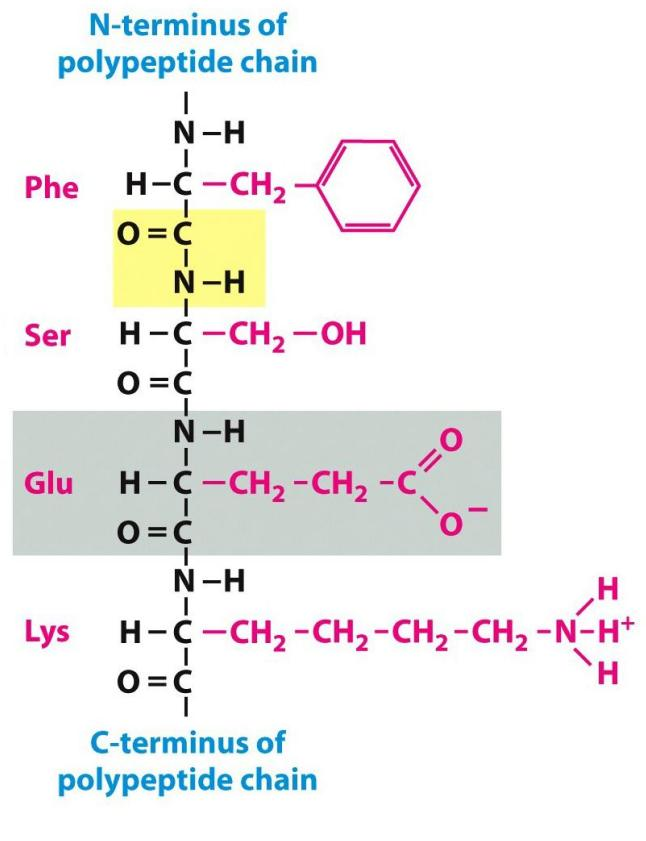
\includegraphics[width=0.6\textwidth]{img/polipeptidoStructure.jpg} 
\caption{Estructura química de un polipéptido} 
\label{polipeptidoEstructura}
\end{figure}



Por definición, una proteína puede estar compuesta por cadenas lineales formadas por cualquier combinación de aminoácidos.
Sin embargo, las proteínas se originan en la naturaleza como producto de los sistemas biológicos, por lo tanto, 
la ocurrencia de las proteínas naturales no se origina por cadenas peptídicas generadas al azar. 
Por el contrario, la ocurrencia de proteínas está ajustada a los requerimientos del sistema y al mecanismo evolutivo subyacente. 
Por lo tanto, el resultado es conjunto de proteínas con un perfil complejo donde cada una tendrá características únicas que determinan su actividad biológica dentro del sistema.
Basándose en estas condiciones, las proteínas naturales quedan mejor definidas si se describen las propiedades secuenciales, estructurales y las actividades biológicas asociadas. 

Cada proteína, entonces, quedará definida por el conjunto de propiedades que la describen, no sólo como polímero(secuencia de aminoácidos) 
sino también como módulo del sistema biológico (perfil de conformaciones en el contexto celular/sistémico, funcionalidades, interacciones, adaptaciones a cambios en el entorno, etc). 

Si bien cada proteína tendrá algunas propiedades individuales únicas(por ejemplo la secuencia de AAs), 
% el perfil de actividades realizadas por las proteínas no es tan complejo y 
el conjunto de proteínas naturales puede clasificarse 
agrupándolas de acuerdo a propiedades secuenciales y conformacionales, donde cada clase está asociada a cierto perfil de actividades biológicas que se derivan de estas propiedades.
En las próximas secciones de este capítulo, cuando se describan alguno de los elementos proteícos naturales, 
se detallarán las propiedades secuenciales y conformacionales asociadas y el perfil de actividades biológicas que realizan.









\subsection{Estructura modular de las proteínas}

Las proteínas naturales son usualmente modulares, conteniendo regiones definidas asociadas cada una con una subfunción específica.
Esta naturaleza modular provee muchas ventajas, principalmente la posibilidad de desarrollar funciones que requieren cooperación de distintos módulos, y un incremento en la estabilidad de la estructura global.
Otra ventajas incluyen la protección de los metabolitos intermedios dentro de espacios inter-dominio, aumentando la eficiencia global y previniendo la liberación al medio de intermediarios inestables de la reacción.  
Desde el punto de vista evolutivo, la modularidad en las proteínas incrementa la capacidad evolutiva reduciendo las restricciones necesarias 
para la adaptación y permitiendo que módulos preexistentes puedan funcionar en nuevos contextos para nuevos usos.

El módulo o unidad de proteína más común es el dominio, el cual puede adquirir distintas definiciones según las propiedades que se analicen:
Podemos definir a un dominio como una unidad evolutiva independiente que puede dar una proteína mono-dominio o formar parte de una multi-dominio. 
Cada unidad(dominio) puede tener una función independiente o contribuir a la función global de una proteína multi-dominio cooperando con el resto de las unidades.
Esta definición de dominio como unidad evolutiva es la que se usa como mecanismo de clasificación en la base de datos SCOP(Structural Classification of Proteins)\cite{murzin1995scop}. 

A diferencia de esto, en CATH\cite{orengo1997cath}, los dominios se definen basándose en conceptos puramente estructurales. 
De esta forma, los dominios pueden definirse como porciones de la secuencia de un polipéptido que pueden asumir una estructura tridimensional estable de forma independiente. 

% La idea de dominio como unidad componente de las proteínas, que se origina en los primeros estudios que se hicieron sobre las proteínas.
Los dominios, si bien son los componentes mas estudiados de la proteínas, no son los únicos componentes, existiendo otras unidades que pueden estar 
limitadas por regiones más cortas e incluso limitarse a simples motivos secuenciales compuestos de unos pocos residuos contiguos.
Cada tipo de módulo tendrá sus propiedades distinguibles.

La arquitectura de las proteínas, entonces, estará dada por la combinación de distintos módulos identificables por sus propiedades secuenciales, estructurales o actividades biológicas características, 
posiblemente unidos por regiones secuenciales que pueden no tener una función de forma individual pero que en conjunto hacen a la actividad biológica global de la proteína.

En la figura \ref{arquitectura} se muestra esta composición modular en un conjunto de proteínas efectoras de bacterias.
La representación gráfica de dominios y motivos con colores permite identificar módulos individuales que pueden repetirse en distintas proteínas.

\begin{figure}[htbp,centered]
\centering
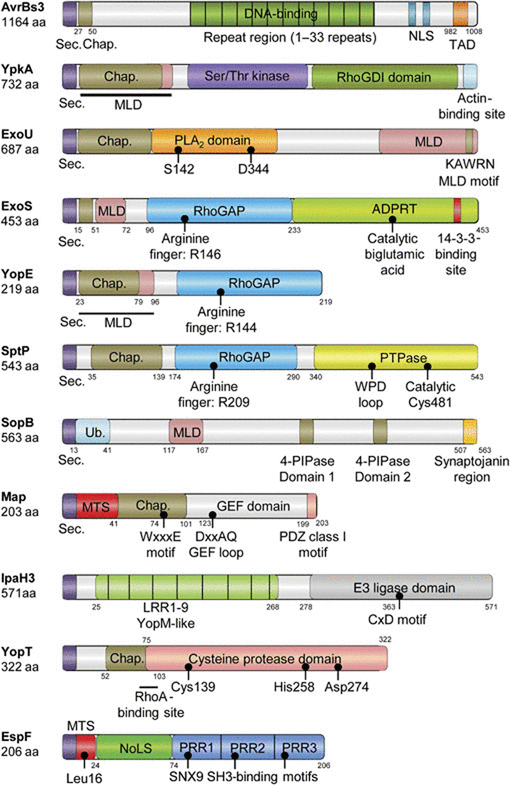
\includegraphics[width=0.6\textwidth]{img/architecture.jpg} 
\caption{Arquitectura de un conjunto de proteinas efectoras de bacterias. Algunos dominios identificables son: Sec. = secretion domain; Chap = chaperone-binding domain; PRR = proline-rich repeats. 
Se identifican otro tipo de módulos, por ejemplo motivos que pueden estar en cualquier parte de la secuencia. Figura extraída de \cite{dean2011functional}} 
\label{arquitectura}
\end{figure}









\subsection{Módulos proteicos} \label{modulosProteicos}
\subsubsection{Proteínas globulares}

% ESTRUCTURA
Las proteínas globulares son los compuestos proteicos más estudiados. En términos generales, estas proteínas se caracterizan por adoptar en condiciones nativas una conformación plegada compacta, 
dándole un aspecto globular y haciéndola soluble en el medio acuoso de la célula.




El hecho que sean, probablemente, las proteínas más estudiadas tiene que ver con todas estas propiedades estructurales básicas, 
al ser solubles y con una estructura determinada y relativamente estable, fueron las primeras que pudieron ser cristalizadas para luego resolver su estructura mediante difracción de rayos X.
La anotación de las estructuras que se resolvían permitió conocer mas sobre las propiedades estructurales mostrando que las proteínas globulares poseen una gran cantidad de estructuras secundarias interaccionando entre si, 
unidas por regiones de la secuencia con estructura flexible no determinada (ver \ref{globularExample}).

\begin{figure}[h]
\centering
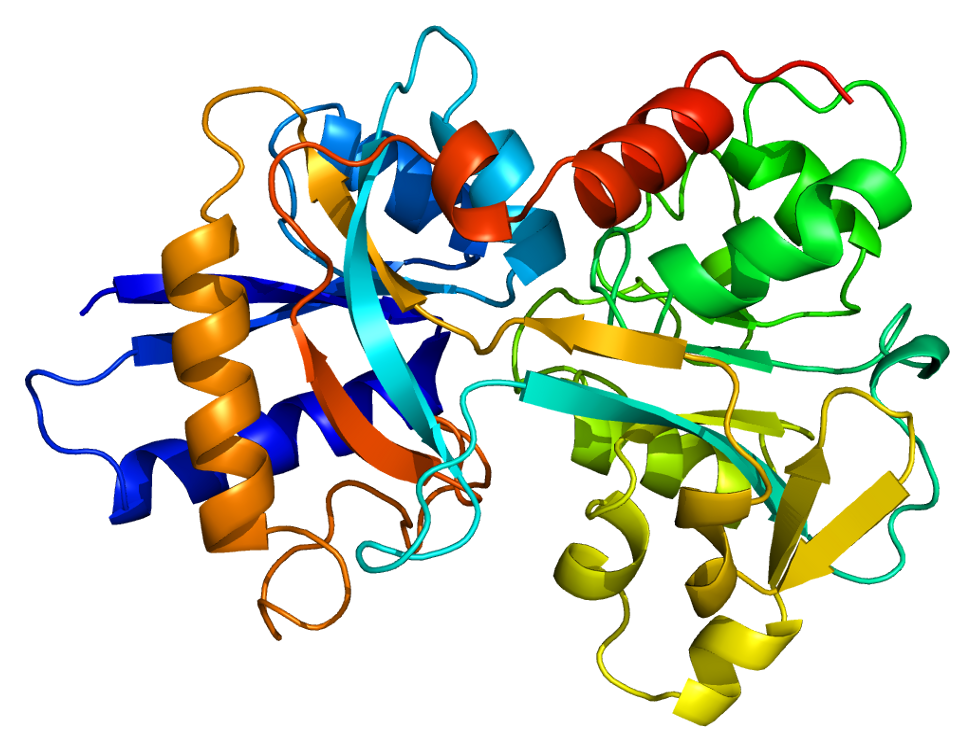
\includegraphics[width=0.8\textwidth]{img/transferrin.png} 
\caption{Ejemplo gráfico de proteína con estructura globular. Imagen de: PDB 1A8E (Transferrin)} 
\label{globularExample}
\end{figure}

Las distintas estructuras secundarias se unen entre si mediante interacciones hidrofóbicas que involucran las cadenas laterales apolares, y por puentes de hidrógeno y a través de interacciones iónicas entre aminoácidos cargados, dando lugar
a la estructura compacta del plegamiento globular. Por lo tanto, el plegamiento adoptado por las estructuras secundarias(estructura terciaria) está intimamente asociado a las propiedades fisicoquímicas de la secuencia. 
En este plegamiento compacto, los aminoácidos más hidrofóbicos quedan alojados principalmente en el interior de la estructura, formando un núcleo hidrofóbico, 
y la superficie globular tiene mayoría de residuos polares, los cuales tienen la capacidad de interaccionar favorablemente con el solvente, lo que lo que le provee la solubilidad característica en el entorno celular. 



La estructura globular puede estar conformada por más de una cadena polipeptídica. En este caso, las diferentes subunidades se unen mediante las mismas interacciones que generan el plegamiento en una cadena, así, 
el plegamiento individual de una cadena puede contener aminoácidos con cadena lateral apolar en alguna región de su superficie, pero esta se complementa con la superficie hidrofóbica de otra cadena cuya interacción mantiene la estructura 
global del complejo.



% ASPECTOS ENERGÉTICOS, TERMODINAMICA Y PROCESO DE PLEGAMIENTO
Todas estas propiedades secuenciales diferenciales a lo largo de la estructura se asocian con el paradigma clásico de la biología estructural, el cual afirma que la secuencia primaria de una proteína 
contiene la codificación para que esta se pliegue adoptando una estructura tridimensional determinada y que, además, la conformación final se corresponde con un mínimo global sobre el perfil de energía libre asociado al polipéptido.  
Esta paradigma se deriva directamente al encontrar que al menos las proteínas pequeñas poseen una tendencia intrínseca a plegarse espontáneamente para dar una única estructura tridimensional.
Los detalles de este proceso de plegamiento, es decir, la forma en que el polipéptido sintetizado por el ribosoma recorre la superficie energética para alcanzar el estado plegado, ha inspirado una gran cantidad de estudios 
aunque aún hoy no se conoce en detalle el mecanismo subyacente.
% AGREGAR FIGURA DE SUPERFICIE ENERGÉTICA DEL PLEGAMIENTO

Teniendo en cuenta que adoptar una estructura determinada en un polipéptido implica un gran costo entrópico, y que las interacciones que describimos como estabilizadoras de este plegamiento son principalmente débiles, 
es de esperar que una característica de las proteínas globulares sea la capacidad intrínseca de su secuencia para formar gran cantidad de interacciones que permitan estabilizar la estructura plegada.





% PARADIGMA ESTRUCTURA FUNCION - PROPIEDADES DINÁMICAS DE LA ESTRUCTURA
El paradigma estructura-función original afirmaba que la función específica de una proteína está determinada por su estructura tridimensional, la cual es única y rígida. 
El origen de este paradigma es el modelo de llave-cerradura propuesto por Emil Fisher el 1894, 
que nace de la necesidad por por explicar la especificidad encontrada en el funcionamiento de diversas enzimas similares por sus correspondientes sustratos. 
La hipótesis utilizada para explicar esto era que la estructura de la proteína(en este caso la enzima) era perfectamente complementaria a la del sustrato correspondiente, en un sistema similar al de una llave en una cerradura.
% Este paradigma extiende los conocimientos vistos previamente acerca de que la secuencia de la proteína tiene codificada la información necesaria para plegarse espontáneamente luego de ser sintetizada en la célula,
% alcanzando esta estructura nativa asociada a la función.
Por un largo período de tiempo, entonces, el modelo de llave-cerradura y el paradigma asociado de estructura-función se mantuvieron como teorías aceptadas, confirmadas continuamente por la
gran diversidad de estructuras que se resolvieron mediante difracción con rayos X. 
% La capacidad de asociar una estructura única, encontrada en el cristal, con la función observada de la proteína en solución reforzaba la idea de una estructura estática asociada a las proteínas

Contrario a este modelo, en 1894 Koshlan sugiere el modelo de encaje inducido, basado en observaciones de enzimas que podían aceptar 
ligandos con diferentes estructuras y, por lo tanto, la proteína debía poseer cierta flexibilidad que le permitiera esta función.
Siguientes evidencias mostraron que esta flexibilidad era parte del mecanismo funcional y que podía implicar cambios conformacionales que van desde variaciones en rotámeros de las cadenas laterales hasta 
reordenamientos conformacionales muy relevantes(por ej. en proteínas alostéricas).
Estas variaciones podian aún ser interpretadas dentro del modelo establecido por el paradigma estructura-función, el cual fue levemente adaptado.
El requerimiento necesario para que la proteína cumpla su función era, entonces, una estructura definida, aunque dinámica. 
Por un tiempo todo pareció indicar(y la mayoría creyó) que una estructura definida, aunque dinámica, era la base del mecanismo funcional.

Si bien esta idea es una simplificación, dado que aún las proteínas mas estables son sistemas dinámicos con distintos grados de flexiblidad, este modelo se adapta a las funciones asociadas a proteínas globulares.
% Comenzaron a surgir, entonces, distintos modelos para explicar cómo la estructura tridimensional confería las propiedades necesarias para  
% Si bien esta idea es una simplificación, dado que aún las proteínas mas estables son sistemas dinámicos con distintos grados de flexiblidad, este modelo se adapta a una gran cantidad de proteínas.
En éstas, el ensamble conformado por los estados accesibles en condiciones fisiológicas está limitado a un conjunto de estructuras que solo difieren en leves desviaciones del promedio del ensamble.
La estructura resultante que se observa de la cristalización es, en realidad, un promedio del ensamble de conformaciones.

La dinámica de estas estructuras está dada por movimientos que van desde fluctuaciones rápidas de pequeña amplitud(del orden de \AA) hasta cambios relativamente lentos($\mu$s - $s$) que 
involucran modificaciones estructurales relevantes(plegamiento y movimientos asociados a la función).
Todos los movimientos son resultantes de rupturas y formaciones de interacciones provocadas por fuerzas de interacción las cuales, debido a su naturaleza débil, pueden romperse 
por efecto de la energía térmica, aún a temperatura ambiente. En general, todos estos movimientos están asociados al mecanismos por el cual ejercen su función.
% Por lo tanto, a pesar de que estas proteínas puedan ser asociadas con estructuras estáticas definidas, las más minimas fluctuaciones térmicas en condiciones normales les permiten
% explorar un conjunto relevante de conformaciones como parte de su actividad biológica.






% % CONCEPTOS EVOLUTIVOS DE LA ESTRUCTURA / SECUENCIA
Sabemos ahora que la funcionalidad emergente de los dominios globulares depende no solo de la estructura promedio del ensamble sino también de los aspectos dinámicos de ésta.
Todas estas características imponen requerimientos al mecanismo evolutivo ya que, para mantener la funcionalidad intrínseca de la proteína, se deben mantener los determinantes secuenciales y estructurales asociados al mecanismo funcional.
Esto impone ciertos requerimientos secuenciales y/o estructurales para la evolución de la proteína, que resulta en una similitud secuencial y estructural entre proteínas homólogas.

Estos conceptos han sido(y son) de gran ayuda en el estudio y clasificación de nuevas proteínas. 
Conociendo la estructura asociada a una proteína se puede inferir la funcion que desarrolla a partir de la búsqueda de proteínas con estructuras similares cuya función sea conocida.
Este mismo método se puede aplicar sobre dominios individuales ya que, como vimos, actúan como unidades estructurales y evolutivas individuales, mostrando funcionalidades independientes.

Incluso cuando no se conoce la estructura, los requerimientos estructurales imponen indirectamente restricciones sobre la secuencia (ya que la estructura es resultado directo de esta).
Estas, junto con ciertos determinantes secuenciales asociados directamente a la funcionalidad, forman un conjunto de restricciones impuesto sobre la evolución secuencial.
De esta forma, el mecanismo de comparación para inferir la funcionalidad puede ser utilizado de forma similar si se comparan las secuencia de una nueva proteína con la de otras cuya función es conocida.
Por lo tanto, la similitud secuencial también permite inferir propiedades funcionales, lo que facilita la anotación de elementos funcionales en secuencias nuevas, aún cuando no se conoce su estructura.

Dado que la secuencia está directamente ligada a la estructura resultante, la similitud secuencial entre proteínas es también un indicio de similitud estructural.
Estos conceptos asociados de propiedes secuenciales, estructurales y funcionales, unidos por el mecanismo evolutivo son las base de gran parte del conocimiento actual sobre proteínas globulares.

% Más alla de esto, los análisis de estructuras existentes asociadas a proteínas globulares permitieron encontrar que hay una gran conservación en los diseños de arquitectura.
% Las combinaciones de estructuras secundarias que daban lugar al plegamiento podían agruparse, entonces, en conjuntos de arquitecturas globales de la proteína que permite
% clasificar y anotar las proteínas de acuerdo a estas arquitecturas resultantes.
% Como resultado de estos analisis estructurales se desarrollaron diversas clasificaciones y bases de datos asociadas. 
% Ejemplo de estas son SCOP y CATH, las cuales se basan en la topología emergente de la combinación de estructuras secundarias propia de la proteína para armar clasificaciones jerárquicas de la arquitectura.
% En el nivel más bajo de la clasificación se encuentran estructuras con gran similitud entre si, indicativo de un ancestro en común y agrupadas generalmente por funciones idénticas o similares.
% % Esta agrupación en ``familias'' con alta  es posible porque, aún cuando la secuencia pueda sufrir mutaciones, la estructura debe conservarse para mantener la funcionalidad.
% 
% % Incluso cuando ....The sequences diverge, but the overall domain architecture remains the same.
% % Particular domains and domain architectures are well conserved over the course of evolution. 






% ACTIVIDADES
Como se menciono previamente el perfil de actividades biológicas asociadas a las proteínas globulares está directamente relacionado con las propiedades conformacionales de estas.
En general, las funciones más estudiadas están asociadas con actividades enzimáticas, donde las proteínas se encuentran generalmente solubles en el medio acuoso de la célula.
La estructura tridimensional definida y gran tamaño que pueden alcanzar estas proteínas también les permite intervenir en actividades que requieren interacciones específicas y estables con otras moléculas, 
ejemplo de esto son los anticuerpos y las proteínas que intervienen en la replicación y reparación del ADN.
El gran tamaño y la solubilidad le permiten actuar como transportadores de otras moléculas con baja solubilidad en medio acuoso.

Las flexibilidad estructural permite que se experimenten cambios conformacionales considerables en la estructura terciaria. 
Dado que las propiedades conformacionales están intimamente ligadas a la funcionalidad, estos cambios, 
que pueden ocurrir como producto de la unión de ligandos o modificaciones sobre químicas dinámicas sin alterar la secuencia, permiten ejercer efectos regulatorios sobre la actividad de la proteína.






% 
% – Flexibilidad
% • No son estructuras rígidas
% • Su flexibilidad depende de un gran número de enlaces débiles
% 
% – Interacciones
% • Unión reversible de ligandos
% • Interacciones reversibles proteína-proteína
% • Se llevan a cabo mediante enlaces débile
% 















\subsubsection{Proteínas de membrana}
Las proteínas de membrana se definen como cualquier proteína que interacciona con la membrana lipídica de la célula.
Algunas de estas proteínas están unidas solo a la superficie de la membrana, mientras que otras tienen regiones que se insertan en el núcleo hidrofóbico(y, posiblemente, también contiene dominios por fuera de éste). 
Se puede hacer, entonces, una primera clasificación en 2 grupos: proteinas integrales y periféricas.

Las proteínas extrínsecas(o periféricas) no interaccionan con el núcleo hidrofóbico y tienen propiedades estructurales y secuenciales similares a las proteínas globulares, 
pero se mantienen en constante interacción con la membrana mediante distintos mecanismos.
Algunas interaccionan indirectamente mediante la unión a proteinas integrales de membrana, otras lo hacen a través de la interacción con los grupos polares que componen las cabezas de los fosfolípidos en la membrana. 
Otro conjunto de proteína periféricas atraviesan procesos de modificaciones post-traduccionales que las unen covalentemente a cadenas carbonadas, las cuales pueden insertarse en el núcleo hidrofóbico y
asi mantener a la proteína en constante interacción con la membrana.
En general, esta clase de proteínas tiene actividades biológicas asociadas a la unión a la membrana, por ejemplo transducción de señales extracelulares, están involucradas en la cadena de transporte de electrones, etc.

% ESTRUCTURA
El otro conjunto de proteínas de membrana son las proteínas integrales(o intrínsecas) tienen uno o mas segmentos insertos en la bicapa lipídica.
En la mayoria, la región insertada atraviesa la membrana (proteínas transmembrana) y tienen dominios intra y extra celulares.
A partir de estos conceptos generales se puede deducir que esta clase de proteínas tendrá una arquitectura/topología particular, donde 

Los segmentos que atraviesan permiten hacer una nueva clasificación por si mismos(ver figura \ref{proteinasMembrana}), así, las proteínas transmembrana se pueden agrupar en dos conjuntos según la estructura que les permite atravesar el núcleo hidrofóbico.
Un primer conjunto de proteínas, las porinas, contienen una estructura característica compuesta por hebras-$\beta$ en una conformación característica con forma de barril que atraviesa la membrana, formando una expansión similar a un poro.
Los aminoácidos de la secuencia son generalmente polares pero, a diferencia de las proteínas globulares típicas, los grupos laterales que están en contacto con la cara externa del barril son hidrofóbicos, y son los que están en contacto con 
los grupos lipídicos, mientras que las cadenas laterales hidrofílicas se encuentran mirando hacia el interior del poro.
La actividad biológica de estas proteínas se deriva directamente de esta estructura, las porinas forman canales en la membrana a través de los cuales distintos metabolitos solubles en agua pueden atravesarla. 

El otro conjunto está dado por aquellas proteínas que contienen hélices-$\alpha$ atravesando una o mas veces la membrana. 
Esta estructura secundaria es la más común entre los segmentos transmembrana ya que permite permite satisfacer todos los puentes de hidrógeno caracterísicos de la estructura carbonada de
the helical structure can satisfy all backbone hydrogen-bonds internally, 
sin dejar grupos polares expuestos hacia fuera de la hélice, y por lo tanto, en contacto con el núcleo hidrofóbico de la membrana

\begin{figure}[h]
\centering
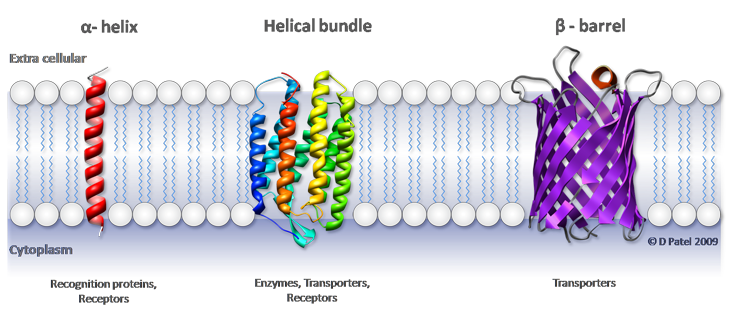
\includegraphics[width=0.8\textwidth]{img/proteinasMembrana.png} 
\caption{Re} 
\label{proteinasMembrana}
\end{figure}


Estos dominios transmembrana tienen, por lo tanto, propiedades secuenciales particulares caracterizadas por aminoácidos con cadenas laterales hidrofóbicas que les permiten interaccionar con el núcleo de la membrana.
% y, generalmente, también con los grupos polares en las superficies de ésta.
Un ejemplo común de este tipo de proteínas es la glicoforina, que contiene un segmento con estructura de hélice-$\alpha$ compuesto totalmente de residuos hidrifóbicos. 
Esta hélice hidrofóbica está, además, rodeada por segmentos flanqueantes conteniendo aminoácidos cargados que interaccionan con las cabezas polares de los fosfolípidos y previenen que la proteína se deslice,
manteniéndola inserta en la membrana.
% Las propiedades hidrofóbicas de su superficie, la flexibilidad que poseen en sus estructuras de forma aislada(no insertadas en la membrana) y los bajos niveles de expresión hacen que sean difíciles de cristalizar.
% Por lo tanto, el estudio de sus estructuras siempre estuvo retrasado con respecto al de las proteínas globulares.
Dentro de este último conjunto existe una gran cantidad de proteínas que contienen múltiples hélices-$\alpha$ transmembrana. Estás proteínas generalmente están conformadas de 2 hélices(formando una estructura tipo coiled-coil)
o 7 hélices(en un arreglo característico de proteínas como la rodopsina).

Estas particularidades en la secuencia permiten distinguirlas fácilmente de, por ejemplo, las proteínas globulares. 
Además, a partir de estos módulos transmembrana y extra/intra celulares se pueden clasificar estas proteínas según la arquitectura o topología global, de acuerdo al número y tipo de segmentos transmembrana, etc.



















\subsubsection{Proteínas intrínsecamente desordenadas}


%  CONCEPTOS GENERALES, SIMPLEMENTE PARA INDICAR QUE NO TIENEN UNA ESTRUCTURA TRIDIMENSIONAL DEFINIDA
% ******************************
Los conocimientos acerca del proceso de plegamiento y la estructura resultante derivados de proteinas globulares formaron, durante un largo tiempo, ideas que se creían aplicables a todas las proteínas existentes.
Con el tiempo se encontraron proteínas que, al parecer, ejercían su función sin tener una estructura tridimensional determinada. 
Estas ideas no se adaptaban a las características de plegamiento y al paradigma estructura-función reinante, por lo tanto, fueron identificándose 
y estudiándose experimentalmente una a una, tratándolas como excepciones al modelo clásico.
Luego de este proceso, hace al menos una década, se formalizó la idea que el estado adoptado en condiciones nativas(funcionales) de muchas regiones o proteínas enteras podía ser intrínsecamente desordenado
(IDRs/IDPs = intrinsically disordered regions/proteins, a partir de ahora). 
% Es decir, existe un conjunto cada vez mas amplio de proteinas cuya secuencia no codifica un plegamiento determinado.



% Inicialmente, gran cantidad de evidencia soportaba la idea que la funcionalidad de las proteínas estaba asociada a su estructura tridimensional bien definida pero dinámica.
% Al no tener una estructura tridimensional determinada, el paradigma reinante que implicaba la necesidad de ésta para poder cumplir alguna función biológica no permitía incluirlas como parte del proteoma.
% Consecuentemente, la idea de que muchas proteínas o regiones no adopten una estructura definida y posean una conformación intrínsecamente desordenada se creyó inaceptable. 
% Estamos hablando de un numero considerable de proteinas cuya secuencia encodes for the intrinsically unstructured proteins without specific structure.
Este reconocimiento trajo consigo una gran cantidad de preguntas, relacionadas con las características estructurales de éstas:
¿Que tan desordenadas/desplegadas son estas proteínas?, ¿Son realmente conformaciones aleatorias o conservan una estructura residual?
¿Si poseen una estructura residual, cómo se clasifican sus conformaciones?
Los avances sobre estas preguntas iban mas allá de las técnicas de resolución estructural conocidas que estaban basadas en el promedio del ensamble, quedando, entonces,
a la espera de aproximaciones/conocimientos provenientes de nuevas técnicas del campo de la biofísica\cite{eliezer2009biophysical}.




\begin{figure}[h]
\centering
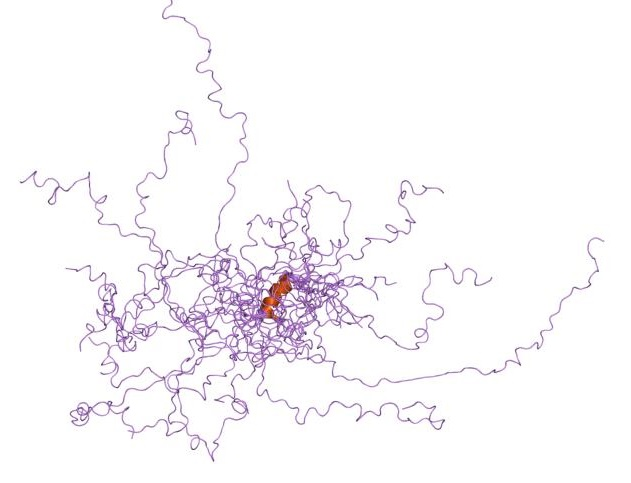
\includegraphics[width=0.8\textwidth]{img/idpExample-TSP9.jpg} 
\caption{NMR structure of the Thylakoid soluble phosphoprotein TSP9, intrinsically disordered protein. Ref:  Micelle-induced folding of spinach thylakoid soluble phosphoprotein of 9 kDa and its functional implications. Biochemistry} 
\label{idpExample}
\end{figure}



% ******************************
% PROPIEDADES ESTRUCTURALES
% ******************************

% CONCEPTOS GENERALES !!! REESCRIBIR-REORDENAR

Este conjunto de proteínas desordenadas se caracteriza la tendencia a adoptar conformaciones extendidas con bajo contenido de estructura secundarias.
La principal característica distintiva de las IDPs es, entonces, su inhabilidad para plegarse en una estructura tridimensional única.
En algunos casos, sin embargo, pueden formar estructuras desordenadas pero compactas, y algunos segmentos de la secuencia pueden adoptar transitivamente estructuras secundarias individuales.
Como vamos a ver, esta leve estructura residual(latente o transitiva) es muy importante y representa gran parte de las capacidades funcionales en IDRs/IDPs.
A pesar de esta tendencia desordenada, debido a la naturaleza heteropolimérica de las proteínas, es probable que las IDPS adopten conformaciones totalmente aleatorias(donde las conformaciones solo estan restringidas por impedimentos estéricos),
aún en entornos altamente desnaturalizantes donde normalmente se pierden las propiedades estructurales.
Por lo tanto, se puede ver que las IDPs poseen propiedades conformacionales complejas, y que esta 
excepcional heterogeneidad estructural representa tambien un problema crítico a la hora de estudiarlas experimentalmente y caracterizarlas.
% Por lo tanto, se puede decir que las IDPs poseen propiedades conformacionales mucho mas complejos que polipéptidos con estructuras totalmente aleatorias y que esta 




% Thus, coil-like ID proteins are not completely random, but are characterized by the presence of some residual (and highly flexible) structure. 

% A partir de esta descripcion estructural se puede entender por qué el término inicial asignado a estas proteínas (proteínas desestructuradas) ha quedado obsoleto.

% A pesar de esta falta de estructura única definida, como se vió, presentan una gran diversidad de propiedades estructurales y, lo que es mas importante, estas están relacionadas con las funciones de la proteína. 
% Por lo tanto, el término general para describir estas proteínas es, simplemente, ``desordenadas''. 
% Este término se aplica tanto a las regiones que forman parte de proteinas plegadas mas grandes, como a secuencias que carecen totalmente de estructura plegada. 
% Como veremos, el mosaico estructural que ofrece la variedad de secuencias conformadas por regiones con propiedades estructurales diversas es fundamental para obtener el extenso catálogo de funcionalidades existentes.    



% Ahora que sabemos que las IDRs/IDPs no están completamente libres de restricciones estructurales, nos concentraremos en describir cuales son las características de su conformación:
Una característica resultante de estas propiedades es que las IDPs poseen conformaciones altamente dinámicas con estructuras que se interconvierten en diferentes escalas de tiempo. 
Estas estructuras varían desde estados completamente sin estructura(polipéptidos nativos sin plegamiento) hasta estados parcialmente plegados(sin estructuras secundarias definidas), o incluso ensambles desordenados pero con ciertas
estructuras secundarias claramente determinadas.
La distribución de estas estructuras está cambiando continuamente en el tiempo, es decir, la estructura tridimensional que podemos ver en un instante dado será diferente de la que veremos en otro momento.

% A pesar de esta dinámica estructural, sin embargo, las IDRs/IDPs carecen de cualquier tipo de estructura secundiaria(o terciaria) estable bajo condiciones fisiológicas.
% Las estructuras residuales que describimos como parte del ensamble, a pesar de ser transitorias, tienen un papel relevante en el cumplimiento de la función asociada a la proteína.
% Cualquier IDR/IDP contiene una gran cantidad de este tipo de elementos estructurales, algunos con gran potencial para plegarse, otros con capacidades de plegamiento diferencial(en algún contexto determinado) 
% y otros sin posibilidad alguna de adquirir una estructura determinada.
% De esta última descripción se puede imaginar que, probablemente, ningún IDR/IDP adoptará una conformación totalmente desordenada a lo largo del tiempo(aunque tampoco estará completamente plegada), por el contrario, se tendrá una gran variedad
% de posibles mosaicos con distintas proporciones y tipos de elementos estructurales.


Estas propiedades dinámicas se pueden entender fácilmente a partir del perfil energético característicamente asociado a estas proteínas.
% En la parte derecha de la figura \ref{idpBindingEnLandscape} se representa gráficamente el perfil energético asociado a estas propiedades conformacionales.
Como se puede ver en la figura \ref{idpBindingEnLandscape}, el paisaje entero queda descrito por una superficie semiplana con múltiples conformaciones asociadas al mínimo de energía, 
con valores de energía aproximadamente iguales y separados por barreras energéticas muy pequeñas.
Estas barreras representan las transiciones rápidas y frecuentes entre las distintas conformaciones que resultan en las propiedades observadas experimentalmente
en solución: un conjunto heterogéneo de conformaciones fácilmente maleable por cambios en el medio. 
En base a esto, se ve que una descripción detallada de IDPs requeriría conocer el ensamble de estados posibles junto con las velocidades de interconversión entre estos.
Todas estas propiedades y las velocidades de las transiciones en el ensamble son difíciles de capturar experimentalmente(y computacionalmente también), aún usando técnicas experimentales que no se basan en promedios de conformaciones.
Los estudios sobre este tipo de proteínas, entonces, se han enfocado en analizar los estados termodinámicamente accesibles como entidades discretas.
Esta idea, si bien sabemos que es una descripción incompleta, permite modelar de forma discreta los elementos funcionales relevantes, sirviendo como base para estudios posteriores.
Este modelo puede extenderse si se representan también las probabilidades de ocurrencia para distintas conformaciones individuales en el ensamble, obteniendo asi un modelo mas dinámico del sistema.



% ***************
%  INDUCED FIT:
% ****************
% Además, este perfil energético se ve modificado por distintas condiciones como modificaciones post-traduccionales, condiciones del medio, presencia de ligandos,etc.
Además, estos ensambles conformacionales dinámicos pueden verse modificados por distintas situaciones como cambios en las condiciones del entorno, modificaciones post-traduccionales, presencia de ligandos, etc.,
lo que modifica no sólo los estados accesibles, sino también la distribución de poblaciones que se encuentran en cada uno.
Una propiedad particular dependiente del contexto, encontrada en los ensambles conformacionales asociados a IDPs, es la capacidad de adquirir nuevos elementos estructurales ordenados estables luego de la unión a ciertos ligandos
(proceso conocido como textit{binding \& folding}\cite{dyson2005intrinsically}). 
Esta propiedad se hace mas relevante de investigar cuando se sabe que, generalmente, está asociada a su funcionalidad biológica y ocurre previamente o durante la realización de esta función.
% Although disordered proteins exist as dynamic structural ensembles without fixed(estable!!!) tertiary structures, there is evidence that many flexible regions of proteins undergo coupled binding and folding \cite{dyson2005intrinsically}. 
% A large decrease in conformation entropy accompanies such disorder-to-order transitions. 

Una gran cantidad de IDPs, entonces, se ven estabilizadas termodinámicamente mediante la unión a ligandos específicos(generalmente otras proteínas, DNA, membranas, etc)
% In other words, intrinsically unfolded proteins in vivo are likely to be stabilized by functional binding to specific targets and ligands 
% (such as a variety of small molecules, substrates, cofactors, other proteins, nucleic acids, membranes and so on). 
% Many intrinsically disordered proteins undergo transitions to more ordered states or fold into stable secondary or tertiary structures on binding to their targets — that is, they undergo coupled folding and binding processes.
Los complejos funcionales entre IDPs y sus ligandos son formados por interacciones intermoleculares específicas y modifican el paisaje energético visto previamente, generando nuevos estados definidos de mínima energía.
Esta diferencia se ve en la región izquierda de la figura \ref{idpBindingEnLandscape}.


\begin{figure}[h]
\centering
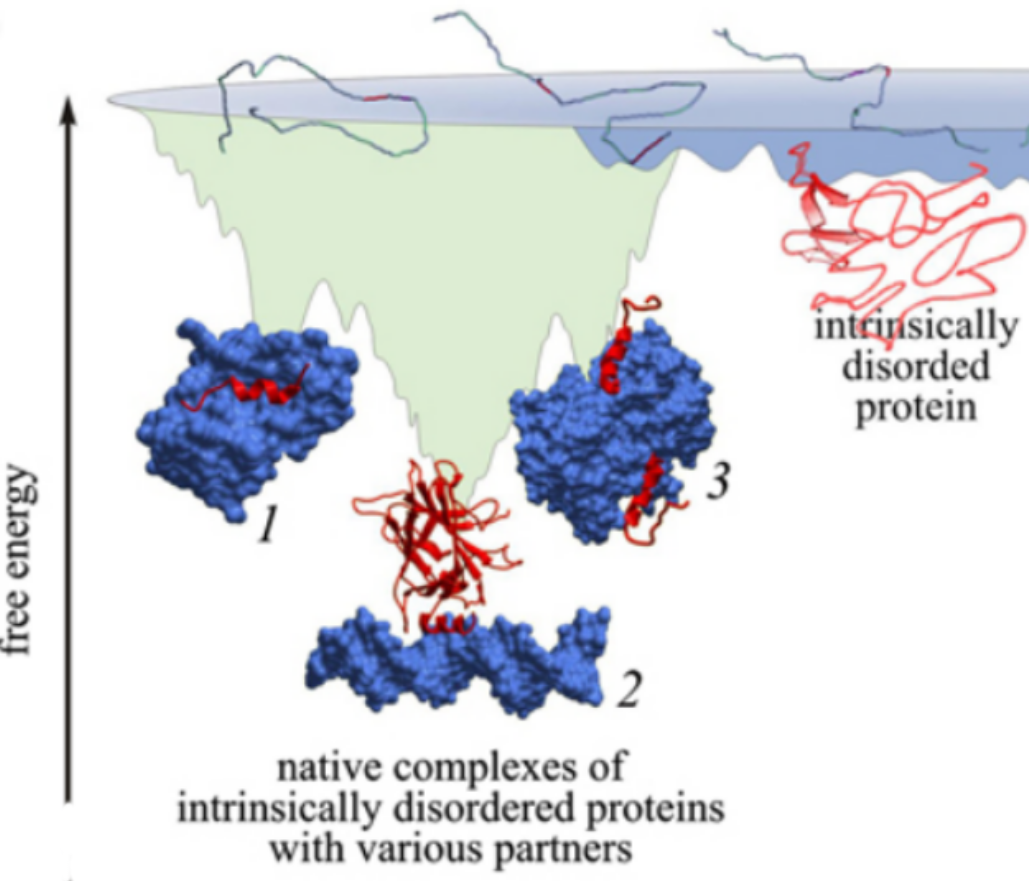
\includegraphics[width=0.7\textwidth]{img/idp-binding-EnLandscape2.png} 
\caption{Perfil energético de los estados de IDRs/IDPs. Los segmentos desordenados pueden plegarse para dar estructuras ordenadas estables a través de interacciones con ligandos específicos.
Esta situación se da cuando la formación del complejo resulta en una disminución de energía libre. 
% Disordered segments of these proteins can gain ordered structure at the interaction with specific binding partners in a case if the free energy of such complexes is lower 
% than the free energies of the intrinsically disordered protein and its partner. 
Por si sólo, el polipéptido presenta un paisaje energético semiplano(sección derecha). La interacción con distintos ligandos(1,2,3) resulta en nuevos estados termodinámicamente estables.
Figura extraída de \cite{turoverov2010protein}}
\label{idpBindingEnLandscape}
\end{figure}

Las IDPs pueden adoptar esta conformación plegada si la energia del complejo formado es menor que la energía libre correspondiente al segmento desordenado y su ligando, previo a la interacción.
% IDPs fold as a whole while interacting with their partners, if the free energy of complex is lower than the free energies of IDP and its partner before their interaction.
En general, sólo un segmento desordenado con características anfipáticas es el que está involucrado en el proceso de unión y plegamiento, en este caso el segmento se denomina elemento de reconocimiento(RE=recognition element). 
% More often, however, only a part of an IDP, a specific recognition element, which is a relatively short amphipathic linear motif contained within long disordered sequence, is involved in the coupled folding and binding events
% Induced fit interactions can also occur between structural domains and relatively large natively unstructured regions of other proteins. 
% The natively unstructured region is then induced to form a stable structure, but only in the presence of the interacting structural domain.
Este tipo de transiciones ante la unión a ciertos ligandos, involucrando regiones cortas de la secuencia, provee una combinación de alta especificidad y baja afinidad que hace a este tipo de elementos extremadamente útiles en procesos de señalizacion y regulación.
% This disorder-to-order transitions, in turn, leads to a combination of high specificity and weak affinity, a pair of linked features that are extremely useful for signalling and regulation.

Una pregunta que aparece naturalmente al intentar estudiar este proceso es si el elemento estructural ordenado es generado durante la unión al ligando 
o si pertenece al conjunto de elementos estructurales encontrados transitivamente en las IDRs/IDPs y, al unirse, se hace parte de la conformación estable.
% An often-raised issue with respect to IDP binding is whether folding occurs before or after binding (termed conformational selection and induced folding, respectively).
% Detailed studies suggest that folding can occur both before and after binding in distinct cases
Estas dos opciones se reflejan en los modelos de selección de conformación y el de unión y plegamiento simultáneo.
Obviamente, en la realidad puede ocurrir cualquiera de estos dos mecanismos o una combinación de los dos.
Esto se ve representado en la figura \ref{idpBinding}


\begin{figure}[h]
\centering
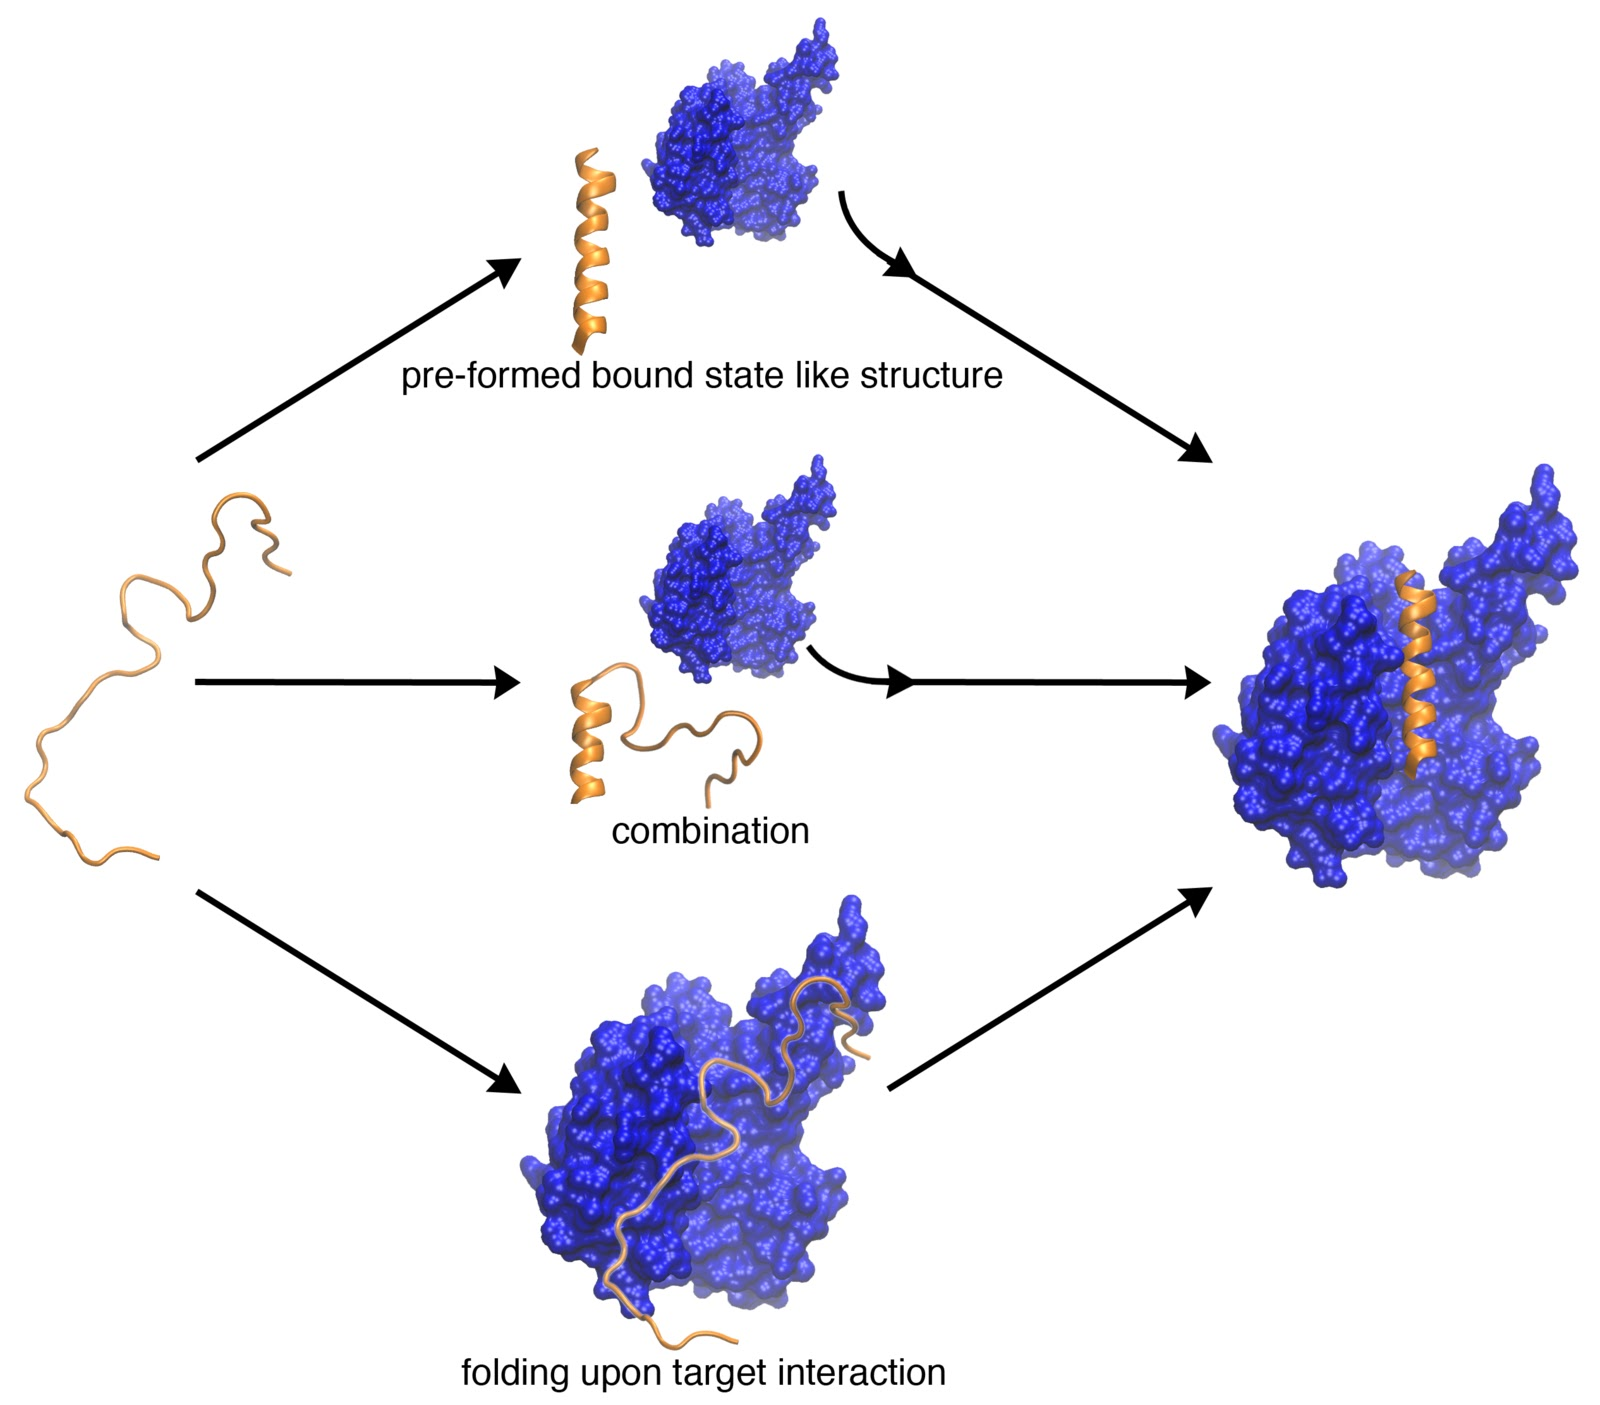
\includegraphics[width=0.8\textwidth]{img/PSE-MoRE.jpg} 
\caption{Distintos modelos de \textit{binding \& folding}} 
\label{idpBinding}
\end{figure}



% ESTO TIENE QUE IR DESPUES DE TODO EL DESARROLLO DE INDUCED FIT
% En base a estas propiedades estructurales y el induced fit, en el review \cite{dunker2001intrinsically} se plantea una clasificacion del desorden en dos categorias: intermittent and constant.
% The former describes protein molecular recognition domains and other regions that undergo order/disorder transitions to carry out binding or other functions. The latter describes regions such as
% proteinaceous detergents, flexible linkers, entropic springs, entropic clocks and entropic bristles that remain disordered while carrying out function.

A partir del estudio sobre este proceso de 'binding \& folding', basándose en los modelos previos, se encontraron algunos conceptos importantes inesperados.
En primer lugar se encontró que dos IDRs/IDPs pueden unirse en un proceso de unión y plegado mutuo \cite{bhattacherjee2012coupled},
es decir, una IDR/IDP también puede funcionar como ligando y plegarse en este proceso. 
Por otro lado, se encontró que el proceso de unión y reconocimiento del ligando puede proceder aún sin necesidad de plegamiento. 
Esto tiene implicancias importantes en los aspectos funcionales ya que, como se había predicho, la capacidad de unión a ligandos dependía de la formación de este elemento estructural.
Gran cantidad de ejemplos de este tipo de uniones(determinados complejos ``fuzzy'') extienden la idea de desorden no sólo a proteínas en solución, sino también a interacciones formando complejos. 









% PROPIEDADES SECUENCIALES
Muchos estudios se hicieron para intentar identificar cómo las características  estructurales tan particulares de las IDPs están codificadas en la secuencia de la proteína.
En el caso de las proteína globulares, la secuencia primaria codifica el proceso de plegamiento y, a través de este, la estructura única final. 
De forma similar, al identificar la IDPs cómo entidades estructuralmente diferenciables, se podría pensar que la estructura primaria de estas determina, también, su falta de estructura tridimensional definida.
Esto tiene como corolario la idea que las secuencias de ambos conjuntos (proteinas ordenadas y proteínas desordenadas) deberían ser diferenciables entre si.
La ausencia de una estructura definida en IDPs es atribuida a las características particulares de sus secuencias de aminoácidos las cuales se describen como secuencias de baja complejidad, enriquecidas en aminoácidos 
cargados y polares, junto con Glicina y Prolina, y un bajo contenido de residuos hidrofóbicos. 
La secuencia suele tener una alta carga neta(positiva o negativa) resultante, o tener segmentos separados de residuos cada uno cargas positivas o negativas.
% Durante el proceso de descubrimiento del conjunto IDPs, muchas proteínas fueron identificadas inicialmente debido a estas simples diferencias en la secuencia.
La relación entre esta combinación de baja hidrofobicidad y alta carga neta y la falta de una estructura definida puede explicarse desde el punto de vista físico:
los altos valores de carga neta producen efectos de repulsión entre las cargas de los residuos, mientras que la baja hidrofobicidad previene la compactación de la estructura lineal
(las interacciones hidrofóbicas son una de las principales fuerzas que interviene en el proceso de plegamiento).
De esta forma, las IDPs no poseen las propiedades secuenciales que le permitan formar suficientes interacciones para estabilizar una estructura compacta con un núcleo hidrofóbico, característica de las proteínas globulares.
% Estas propiedades no solo son necesarias para estabilizar la estructura compacta final sino que también se cree son importantes en el proceso de plegamiento para adquirir esta estructura.
% en un proceso similar a un colapso hidrofóbico. 
El resultado es una estructura con tendencia a mantener una conformación desplegada, característica de las IDPs.

 
% ****SI HACE FALTA PUEDO AGREGAR ESTE PARRAFO SOBRE ALGUNAS CARACTERISTICAS EXTRA DE LAS SECUENCIAS, O REFERENCIAR ALGO, 
% 
% The disordered proteins are significantly depleted in bulky hydrophobic (Ile, Leu, and Val) and aromatic amino acid residues (Trp, Tyr, and Phe), which would normally form the hydrophobic core of a folded globular protein, 
% and also possess low content of Cys and Asn residues.
% The depletion of ID protein in Cys is also crucial as this amino acid residue is known to have a significant contribution to the protein conformation stability via 
% the disulfide bond formation or being involved in coordination of different prosthetic groups.
% On the other hand, ID proteins were shown to be substantially enriched in polar, disorder-promoting, 
% amino acids: Ala, Arg, Gly, Gln, Ser, Glu, and Lys and also in the hydrophobic, but structure braking Pro.


% The fact that natively unfolded proteins, with their depleted hydrophobicity, are noncompact under physiological conditions indicates that ‘salted water’ (typical ‘physiological’ buffer contains 100–150 mM NaCl) does not represent for them a poor solvent.
% In other words, these conditions do not force polymer segments to interact specifically with each other and, thus, do not force them to be effectively excluded from the solvent.
% On the other hand, it has already been noted that even high concentrations of strong denaturants do not represent a good solvent for a polypeptide chain encoding for a typical globular protein, and a globular protein was assumed to never be a random coil.


% Por lo tanto, a signature of probable intrinsic disorder is the presence of low sequence complexity and amino-acid compositional bias, with a low content of bulky hydrophobic aminoacids (Val, Leu, Ile, Met, Phe, Trp and Tyr), which would
% normally form the core of a folded globular protein, and a high proportion of particular polar and charged amino.....
% ESTAS PROPIEDADES SE HAN UTILIZADO PARA LAS PRIMERAS GENERACIONES DE HERRAMIENTAS PARA PREDECIR DESORDEN A PARTIR DE LA SECUENCIA.
% Luego se crearon predictores que analizaban la secuencia usando ventanas(PONDR)

% In addition to amino-acid composition, the disordered segments have also been compared with the ordered ones by various attributes such as hydropathy, net charge, flexibility index, helix
% propensities, strand propensities, and compositions for groups of amino acids such as W + Y + F (aromaticity).

% Estas propiedades fisicoquimicas tambien fueron incluidas para los predictores.













% ACTIVIDADES
% 
% % Como vimos antes, diversos estudios estructurales mostraron que este tipo de conformaciones no solamente existe realmente \textit{in-vivo}, sino que representa el estado funcional de estas proteínas y,
% % dado que la habilidad para realizar su función biológica es lo que distingue al estado nativo, este conjunto de proteínas parcial o totalmente desordenadas debe ser considerada como entidades nativas. 
% Debido a su amplio ensamble conformacional, el cual va más allá de una simple variación/dinámica estructural, el modelo de encaje inducido al cual se adaptan correctamente las proteínas globulares no permitiría explicar el funcionamiento
% de las proteínas intrínsecamente desordenadas.
% Por lo tanto, estas proteínas desafían el paradigma casi dogmático de estructura-función, fuertemente establecido hasta el momento.
% Esto significa que el paradigma estructura-función previo, que implica la indispensable existencia de una estructura ordenada como requisito para una función efectiva, debe ser redefinido para incluir ese nuevo conjunto de entidades
% \cite{wright1999intrinsically}.
% De acuerdo a este nuevo paradigma, las proteínas nativas(o sus regiones funcionales) pueden existir en cualquiera de los estados conformacionales conocidos que se desarrollaron en las secciones previas.
% En la figura \ref{stuctured-idp-functions} se muestra el paralelismo entre los paradigmas descritos y el proteoma resultante.
% 
% 
% \begin{figure}[h!,centered]
% \centering
% 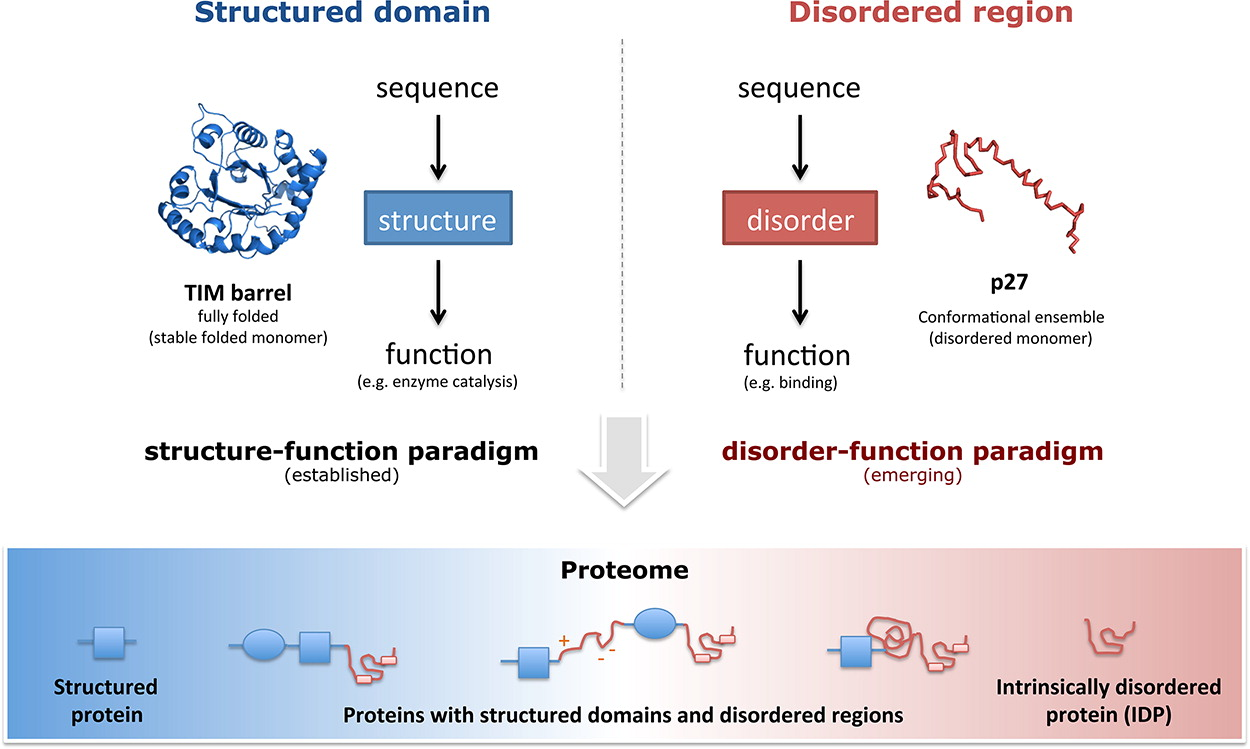
\includegraphics[width=0.9\textwidth]{img/structure-idp-function.jpeg} 
% \caption{Paralelismo entre funcionalidad emergente de dominios plegados y de proteinas/regiones intrínsecamente desordenadas. Figura extraida de \cite{van2014classification}}
% \label{stuctured-idp-functions}
% \end{figure}


% El principal objetivo de todos los modelos y estudios estructurales en estas proteínas es poder elucidar los tipos y modos funcionales subyacentes.
Una pregunta importante que surge de las propiedades estructurales es como estas desarrollan las funcionalidades asociadas y cuales son las funciones fisiológica que cumplen las IDPs.
% El estudio de las funcionalidades provistas por IDPs se ve dificultada por las propiedades intrínsecas de estas proteinas:
% Como se dijo antes, el paradigma inicial de secuencia-estructura-función provee una base para relacionar los conocimientos entre mediante métodos de análisis y anotaciones de secuencias estructuras y funciones.
% Por el contrario, las proteínas dentro de este nuevo conjunto de IDPs se corresponden con un ensamble conformacional heterogéneo.
% Dado que, entonces, no es posible obtener una estructura promedio representativa, es díficil obtener información relevante de la funcionalidad a partir del ensamble conformacional.
% Lo que es más, dada la ausencia de restricciones estructurales, las secuencias de estas proteínas tienden a evolucionar más rapidamente que sus pares ordenados.
% Como resultado, la identificacion de secuencias/regiones homólogas es considerablemente mas difícil.
% Estas consideraciones manifiestan la necesidad de avanzar en el desarrollo de esquemas de clasificación específicos para este nuevo conjunto de proteínas, apuntando a mejorar la predicción funcional y la anotación.
Un paso importante para entender esto es la clasificación de las IDPs conocidas de acuerdo a sus funcionalidades\cite{van2014classification}.
% Como parte de estos avances se han ensayado una gran diversidad de clasificaciones\cite{van2014classification}.
La figura \ref{idpFunctions} detalla la clasificacion de funcionalidades y mecanismos asociados a IDPs junto con las proporciones de instancias encontradas para cada uno.
De esta clasificacion se puede ver que las funcionalidades en las IDPs emergen a partir del propio desorden intrínseco o mediante mecanismos de reconocimiento molecular(interacciones transitivas o permanentes).
% En la figura \ref{proteinMechanisms} se ve una clasificación general bastante simplificada de los roles y mecanismos funcionales generalmente provistos por los distintos tipos de proteinas. 
% En esta clasificacion de proteinas segun su rol general, se incluyen también las proteínas globulares y de membrana que mencionamos previamente(asociadas a actividades enzimáticas, transporte, etc), agrupadas como proteínas plegadas.

En el primero caso, el mecanismo subyacente de funcionamiento no implica ninguna interacción sino que depende directamente de la flexibilidad y plasticidad de la cadena carbonada(\textit{entropic chains}).
En este caso, las proteínas satisfacen un conjunto de requerimientos celulares únicos en los cuales la funcion a cumplir es una consecuencia directa de las propiedades conformacionales que poseen. 
Esta función, generalmente está asociada a secuencias linkers, cuyo objetivo es unir distintos unidades componentes de las proteínas.

En el segundo caso, el amplio perfil de interacciones posibles permite que las IDPs participen en funcionalidades muy diversas, entre estas están la función de chaperonas, la modulación de actividades de otras moléculas(generalmente proteínas) 
y la neutralización de pequeños ligandos uniéndose a ellos.
% El mecanismo asociado a estos generalmente implica el plegamiento para adquirir una estructura ordenada al interaccionar con el ligando.
El mecanismo de reconocimiento e interacción es básicamente diferente a la que adoptan los dominios globulares. 
Mientras que estos últimos han evolucionado para dar una gran variedad de plegamientos diferentes que proveen reconocimientos especificos, 
en IDPs el mecanismo de unión \textit{binding} es principalmente mediado por segmentos cortos de reconocimiento\cite{neduva2005systematic,fuxreiter2007local}, caracterizados por su naturaleza flexible, lo que 
les aporta una gran cantidad de ventajas\cite{gunasekaran2003extended,dyson2005intrinsically}.%REFERENCIA AL PAPER DE MECANISMOS FUNCIOMNALES DE IDPs

% 
% \begin{figure}[h!,centered]
% \centering
% 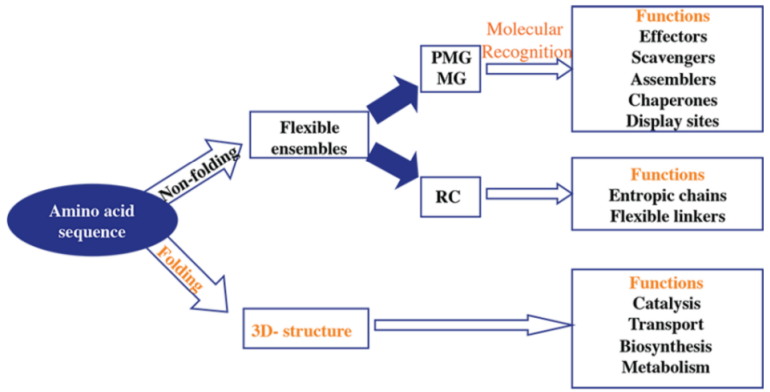
\includegraphics[width=0.9\textwidth]{img/proteinFunctionMechanisms.png} 
% \caption{Distinctive properties of proteins: diversity and functional role. Figura extraida de \cite{habchi2014introducing} }
% \label{proteinMechanisms}
% \end{figure}
% 
% 



\begin{figure}[h!,centered]
\centering
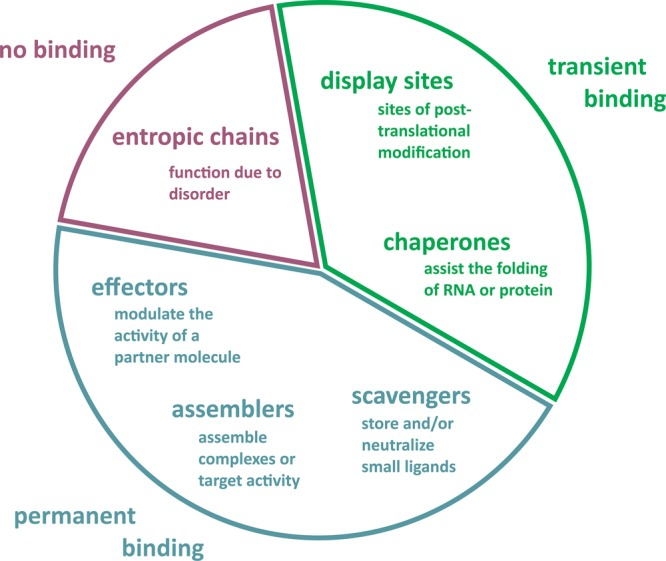
\includegraphics[width=0.7\textwidth]{img/idpFunctionMechanisms.jpg} 
\caption{Clasificación roles y mecanismos funcionales de IDPs/IDRs. Figura extraida de \cite{van2014classification}}
\label{idpFunctions}
\end{figure}


% Para el caso de las proteínas globulares, los dominios son los principales módulos estructurales y funcionales.
% A diferencia de esto, la identificación de las regiones/elementos funcionales dentro de IDPs es un area que todavía está en desarrollo y no es fácil realizar una identificación clara ni mucho menos exhaustiva de éstos. 

% Los elementos asociados al proceso de unión y plegamiento forman el primer conjunto de elementos funcionales 
Dentro de estos segmentos podemos identificar a los elemento de reconocimiento(RE=recognition element)\cite{mohan2006analysis,vacic2007characterization,oldfield2005coupled}, los cuales involucran regiones cortas(10-70 aminoácidos de largo) 
con propiedades generalmente anfipáticas, y se caracterízan porque pueden experimentar un proceso plegado y unión(descrito previamente) que permite la interacción con ligandos.  
% Estos REs(o MoREs por el nombre en inglés de Molecular Recognition Elements) pueden, a su vez, subclasificarse de acuerdo a las estructuras secundarias que adoptan en el complejo de unión. % bound state
% Los dos modelos descritos previamente para el proceso de unión y plegamiento (selección de conformación y unión y plegamiento simultáneo) permiten subclasificar aún más estos elementos desde el punto de vista estructural, 
% agregando el concepto de elementos estructurales preformados(PSEs)\cite{fuxreiter2004preformed}. 
% Estos PSEs se corresponden con el modelo de selección de conformaciones, es decir, son regiones intrínsecamente desordenadas que tienen tendencia a formar elementos estructurales transitivos, adquiriendo temporalmente estructuras secundarias.
% Estos elementos pueden tener la capacidad potencial de servir como sitios de unión y quedar estabilizados en el complejo formado.
% Como primeros elementos funcionales identificados a partir de sus propiedades conformacionales dentro de IDPs tenemos, entonces, a los MoREs y PSEs. 
% Esta clasificación no es totalmente excluyente ya que, como se dijo previamente, puede haber elementos que resulten de una combinacion de estos conceptos.
% 

% ACA CONECTO CON SLM
Más allá de estos elementos que fueron descubiertos a partir de análisis estructurales, el mecanismo de reconocimiento ha sido estudiado desde el punto de vista de los patrones secuenciales que los determinan, 
encontrandose elementos en la secuencia caracterizados por presentar interfaces
de interacción muy compactas (los residuos determinantes de la afinidad y especificidad estan contenidos generalmente en unos 3-11 AAs contiguos).
Estos elementos se conocen como motivos lineales o por sus siglas en inglés, LMs, ELMs, SLiMs o MiniMotifs\cite{davey2012attributes}. 
Como resultado del número limitado de contactos para interacciones con ligandos, los SLMs se unen con una afinidad relativa muy baja lo que resulta en una ventaja considerable 
para participar en interacciones transientes, condicionales y  ajustables, que son propias de los procesos regulatorios.

En términos de funcionalidad, se pueden clasificar los SLMs en dos grandes familias: los que actúan como sitios objetivo de modificaciones post-traduccionales(PTM), 
y los que funcionan como ligandos en la formación de complejos de interacción.
% Dado que el conjunto de funcionalidades y propiedades estudiadas en relación a estos motivos lineales en la secuencia se corresponden en gran medida con las funcionalidades principales de IDRs/IDPs, 
En \cite{fuxreiter2007local} se analizaron los perfiles conformacionales de proteínas que contienen instancias de éstos(no solo la conformación del segmento sino también el contexto), concluyendo que, efectivamente, 
suelen encontrarse formando parte de regiones IDRs y por lo tanto forman parte del conjunto de elementos funcionales característicos de IDPs.
Sin embargo, los SLMs se diferencian de los MoREs descritos previamente en que estos últimos dependen de un patrón de desorden en la secuencia(el cual puede ser obtenido con herramientas de predicción de desorden), 
mientras que los SLMs dependen de motivos secuenciales específicos.

El hecho que esten definidos por solo un pequeño segmento de AAs tiene consecuencias relevantes en aspectos biológicos de los SLM.
En particular, claramente resulta muy probable que estos aparezcan o desaparezcan mediante mutaciones. 
Dado que solo se necesitan un número muy limitado de mutaciones para que surgan, estos son propensos a la evolución convergente, lo que facilita la proliferación en distintos lugares del proteoma.
Esto resulta en una fuente de evolución para la red de interacciones ya que se generan interfaces \textit{de novo} en distintas proteínas.
Estas mismas características dinámicas de la secuencia los hace mas difíciles de estudiar que elementos funcionales mas restringidos evolutivamente como los dominios globulares.
Por lo tanto, a pesar de la disponibilidad de miles de secuencias de proteínas, el descubrimiento de motivos contenidos en estas es aún una tarea difícil.

% SI ENCUENTRO REFERENCIA PARA ESTO LO AGREGO !!!
% Las propiedades de funcionalidad altamente dinamicas y la importancia biologica que tienen estos elementos hacen esperable que esten altamente regulados en la celula.






% *************************************************************
% ******    IDD  ********************
% ACA AGREGO OTRO ELEMENTO, LOS DOMINIOS ID, QUE PUEDEN SER OTRA CLASIFICACION
A pesar que las interacciones mediante SLMs suelen ser débiles, transitivas y, posiblemente, tener baja especificidad, pueden originarse interfaces mas especificas y de mayor afinidad si 
se obtiene cooperación de las regiones flanqueantes, si se combinan varios motivos cortos, o si se utilizan dominios desordenados con mayor longitud.
Es relevante decir que las regiones de unión en IDPs suelen corresponderse mas con dominios que con motivos cortos, teniendo longitudes que exceden los 20-30 residuos
\cite{tompa2009close,chen2006conservation,chen2006conservationB}.  
Además de esta longitud característica, tienen distintas propiedades que los distinguen como dominios:
Son estructuralmente y funcionalmente independientes dentro de la proteína, pueden ser más facilmente reconocibles mediante similitud secuencial debido a que sus secuencias están conservadas, 
y poseen al menos una función específica que los identifica.
Al poder distinguirlos como dominios intrínsecamente desordenados(IDDs) podemos clasificarlos, entonces, como una nueva clase de elementos funcionales independientes que pueden encontrarse dentro de IDPs.
Estos elementos tienen funciones muy diversas pero, generalmente, están involucrados en procesos de interacción con DNA, RNA u otras proteínas.









% 
% % COMENTARIOS APARTE SOBRE LA REGULACION DE IDPs EN LA CELULA
% En términos biológicos las diferencias secuenciales entre las IDRs/IDPs y los segmentos o proteínas totalmente plegadas, además de las diferencias conformacionales antes vistas(y de las diferencias funcionales que veremos), 
% indican que se tratan de entidades separadas dentro del complejo perfil del proteínas naturales existentes.
% Esta claro, además, que no sólo son un elemento real y distinguible, sino que son abundantes en el proteoma, tienen propiedades muy diversas y cumplen funciones vitales para cualquier sistema biológico.
% Todas estas propiedades hacen que parezca razonable que este tipo de proteínas este altamente regulada dentro de la célula \cite{gsponer2008tight,habchi2014introducing}.






% ACTIVIDADES BIOLOGICAS
% 
% Certain biological functions, such as enzyme cat-
% alysis, immunological recognition, or molecular
% discrimination by receptors, absolutely demand
% exquisite control of three-dimensional structure. In
% contrast, functions such as signaling can be
% achieved by linear sequences, simple sequence pat-
% terns, or by isolated secondary structural motifs.
% Intrinsically unstructured proteins, which are
% induced to fold by interactions with other mol-
% ecules, offer several important advantages in sys-
% tems involved in cellular signaling and regulation.
% Unstructured proteins are inherently  ̄exible and
% both their local and global structures can easily be
% shaped by their environment. Such intrinsic plas-
% ticity could allow a single protein to recognize a
% large number of biological targets without sacri®-
% cing speci®city.
% 





























\subsubsection{Agregados proteicos}


% CONCEPTOS GENERALES 

% Las proteínas plegadas, como las proteínas globulares vistas previamente dependen de la estructura  para poder funcionar correctamente, deban atravesar un proceso de plegamiento el cual ocurre, en condiciones normales, de manera muy rápida. 
% Para que los dominios globulares adquieran 
% Esto es posible ya que sus secuencias han evolucionado de forma tal que son capaces de alcanzar la estructura nativa(funcional) muy eficientemente, incluso en el complejo entorno celular.
% Sin embargo, a medida que el tamaño de la proteína aumenta, tambien aumenta la complejidad del proceso de plegamiento y este se vuelve propenso a errores,
% lo que puede llevar a estas proteínas a adoptar conformaciones incorrectas(\textit{misfolded}). 
% Los errores durante este proceso en el que se buscan las interacciones ``correctas'' entre los residuos pueden estar asociados a distintos factores(principalmente mutaciones), 
% no sólo al tamaño de la proteína, ya que de por si el proceso de plegamiento es complejo. 
% Por otro lado, si estos estados estructurales incorrectos mantienen su solubilidad pueden comenzar a acumularse en el entorno celular.
% 
% Ademas de estos estados \textit{misfolded}, algunos intermediarios en el proceso de plegamiento pueden tener tiempos de vida considerables, poblando estados alternativos al plegamiento final.
% Más alla de esto, una vez alcanzada la estructura final, diversas condiciones del entorno pueden producir que este se pierda y se adopte un estado no-plegado(\textit{unfolded}).
% Las proteinas plegadas, entonces, no siempre se encuentran en su estado nativo dentro del entorno celular y pueden ocurrir acumulaciones de estados \textit{misfolded} los cuales, por definición, 
% abarcan a cualquier proteína que no esté en su estado nativo.
% 
% Además del efecto que tiene adoptar un estado \textit{misfolded} sobre la función de la proteína, estos estados pueden también llevar a la formación de agregados entre proteínas
% lo cual tiene, generalmente, un efecto devastador en la célula/organismo.
% A pesar que hemos utilizado el concepto de \textit{misfolding} para introducir la problemática de agregación, estos dos procesos no son necesariamente dependientes entre si, y los agregados representan componentes proteicos mucho 
% mas complejos que la simple acumulación de estados no-nativos, pudiendose originar a partir de diversos estados iniciales mediante procesos que aún hoy son sujeto de estudios, resultando en conformaciones estructurales muy diversas.
% Como se verá, la habilidad de una proteína a formar distintos tipos de agregados depende de muchos factores, entre los cuales están claramente la secuencia y el entorno en que se encuentra,
% de otra forma, las proteinas que adquieran conformaciones no estructuradas o que se encuentren en estados de plegamiento intermedios semi-estables tendrían una tendencia mucho mayor a la agregación y, sin embargo, esto no es así. 

En términos generales, los agregados proteicos se forman por la asociación(interacción) anormal entre proteínas, dando complejos con distintas propiedades y que pueden acumular una gran cantidad de proteínas.
Si bien algunos agregados pequeños pueden mantenerse en solución, en general terminan formando precipitados en condiciones fisiológicas. 

A partir de las características morfológicas de estos, se pueden distingir escencialmente dos tipos: agregados amorfos y fibrillas amiloides.
Los primeros muestran una apariencia granular y consisten principalmente de proteínas en conformaciones desplegadas, aunque presentan ciertas regiones cierto enriquecimiento de estructuras de hoja-$\beta$ plegada, las cuales
mantiene las proteínas unidas formando el agregado.
Por otro lado, las fibrillas amiloides poseen estructuras altamente ordenadas y repetitivas donde todos los polipéptidos que la componen adoptan un plegamiento en común.
% Si bien no nos vamos a enfocar en los detalles puntuales de la estructura, se sabe que 
Estas diferencias que se ven en la conformación macromolecular son el reflejo de diferencias en las interacciones y arquitectura a nivel atómico.
Por otro lado, las diferencias estructurales también se reflejan a nivel biológico: los distintos tipos de agregados tienen afinidades diferentes frente al conjunto de chaperonas y, además, 
pueden acumularse en diferentes localizaciones celulares y ser degradados por mecanismos diferentes.
% Por último, a diferencia de los agregados amorfos, las propiedades únicas de las fibrillasas amiloides han sido aprovechadas por 
% distintos sistemas biológicos y pueden encontrarse versiones funcionales de éstas en distintos organismos\cite{fowler2007functional}.

A pesar que podría parecer obvio, es importante diferenciar los precipitados en los que las proteínas mantienen su estructura nativa de estos agregados que surgen a partir de nuevas estructuras no-nativas.
La precipitación es generada por la inducción de un entorno de solubilidad reducida, por ejemplo durante la precipitación isoeléctrica o mediante sulfato de amonio,
que son los procesos típicos para obtener los cristales utilizados en la resolución de estructuras por difracción de rayos X. 
En estos casos, la reducción de la fuerza iónica o el cambio en el pH de la solución restituye los precipitados a la forma soluble.
El segundo tipo de estructuras macromoleculares representa la formación de interacciones entre proteínas(principalmente formando hojas-$\beta$) que llevan a la formación de estados muy estables, 
reflejados en un profundo mínimo sobre el perfil de energía correspondiente. 
Esto hace que solo sea posible restituir la forma soluble de los componentes mediante procedimientos extremos aunque, igualmente, es dificil que las proteínas vuelvan a adoptar sus conformaciones nativas.
% permanenciendo en solución aconformaciones mal plegadas.
Este tipo de agregados es de nuestro mayor interés en el trabajo ya que puede ocurrir en condiciones experimentales ``normales'', que no han sido inducidas con el fin de formarlos.


En el gráfico \ref{aggregationDiagram} se muestran distontos agregados proteícos, integrados dentro del perfil conformacional de las proteínas, mostrando los distintos tipos de estructuras de agregación, 
los intermediarios a partir de los cuales se originan, y los equilibrios y mecanismos para desintegrarlos. 


\begin{figure}[h!,centered]
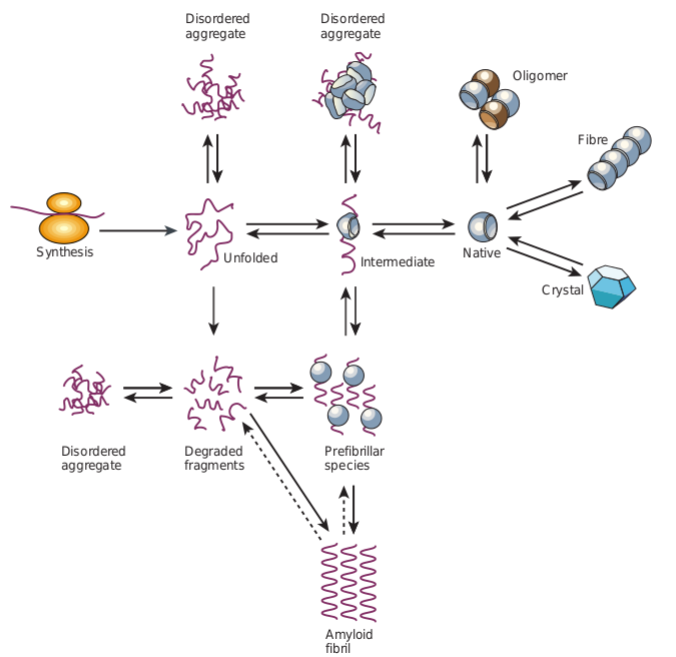
\includegraphics[width=\textwidth]{img/aggregationDiagram.png} 
\caption{} \label{aggregationDiagram}
\end{figure}



% ESTRUCTURA
Las fibrillas amiloides son, probablemente, el tipo de agregado más interesante y el más estudiado, ya que tiene propiedades que las hacen muy particulares.
En primer lugar, como se mencionó antes, adoptan estructuras altamente ordenadas y compactas, similares en parte a los estados nativos de proteinas globulares.
Por otro lado, parte de las propiedades únicas de este tipo de estructuras es que, probablemente debido a su estructura de puentes de hidrógeno altamente organizada, posee una estabilidad cinética única.
Por lo tanto, una vez formados estos agregados pueden mantenerse durante largos períodos de tiempo, funcionando como núcleo para la agregación de más cantidades de la misma proteína 
y permitiendo la formación de depósitos en la célula/tejido.

La formación de agregados amiloides fue observada por primera vez en el contexto de la amiloidosis sistémica hace mas de 150 años y, de hecho, obtuvo su nombre en este descubrimiento cuando se encontró que 
los depósitos observados respondían a la tinción con iodo, el colorante usado para la deteccion de almidón. 
Desde entonces, se encontró que los depósitos de proteínas encontrados en distintas enfermedades provocadas por \textit{misfolding} de proteínas poseían estas características amiloides.
Estos depósitos estaban conformados generalmente de un solo tipo de proteínas, aunque se encontraban \textit{in-vivo} asociados a distintas moléculas.
Los estudios más avanzados de su estructura revelaron las características altamente ordenadas, compactas, estables y no-ramificadas que poseen estos agregados y que se ven reflejados en
la morfología fibrilar que puede apreciarse al verlos mediante el microscopio electrónico de transmisión.
El diámetro de estas estructuras fibrilares(fibrillas) se encuentra en el rango de los 10 \textit{nm} y su longitud puede alcanzar varios micrómetros. 
Estas fibrillas maduras pueden, además, asociarse lateralmente entre si para formar fibras.

Todas las fibrillas amiloides comparten una arquitectura en común compuesta de una estructura suprasecundaria de unión entre hojas-$\beta$.
Los detalles de esta arquitectura, obtenidos mediante difracción con rayos X, revelan que 
las hojas-$\beta$ se extienden con las caras de sus hebras enfrentadas entre si pero perpendiculares al eje de la fibrilla que forman\cite{nelson2005structure}.  
Esta arquitectura de hojas-$\beta$ cruzadas permite, como se mencionó antes, la formación de un continuo de puentes de hidrógeno que provee a estas componentes de gran estabilidad. 
En la figura \ref{amyloidStructure} se ve una representación gráfica detallada de esta estructura.



\begin{figure}[ht]
\centering
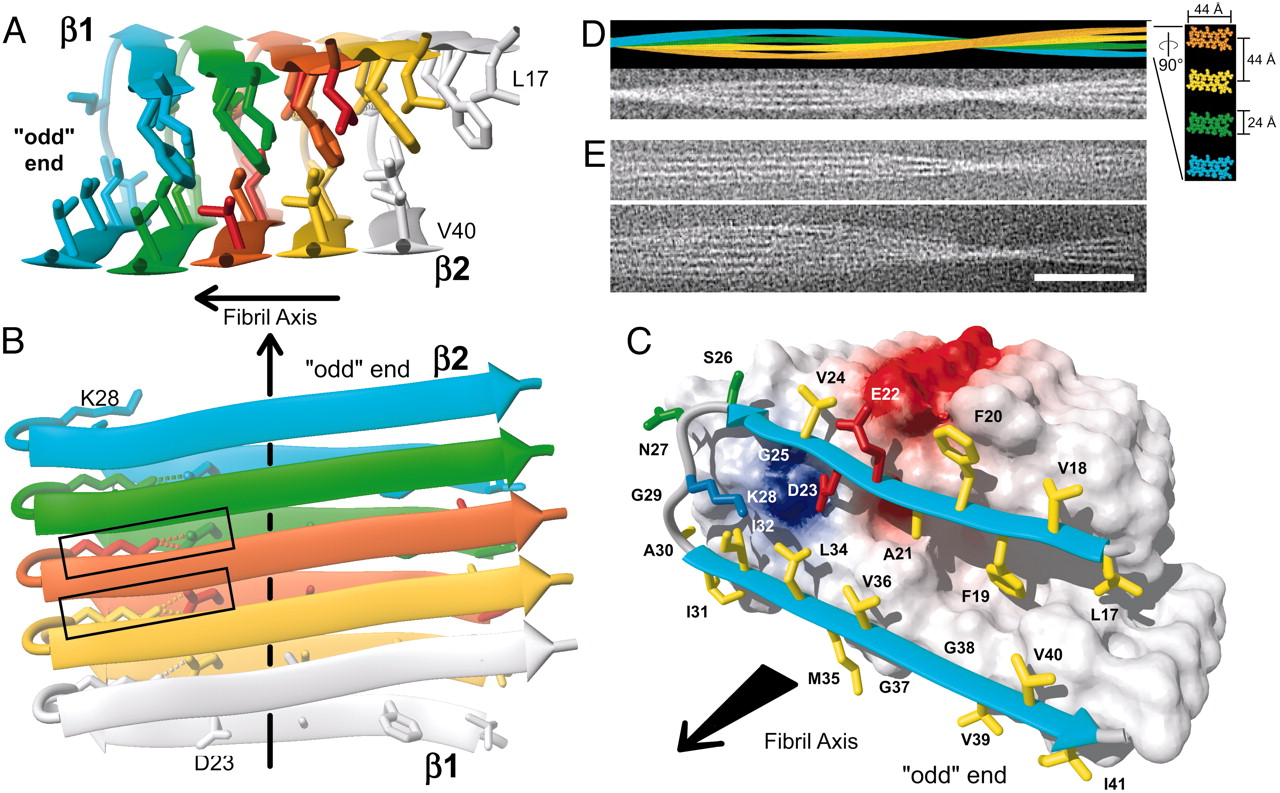
\includegraphics[width=0.9\textwidth]{img/amyloidStructure.jpg} 
\caption{Estructura de fibrillas amiloides. Figura extraída de \cite{luhrs20053d}}
\label{amyloidStructure}
\end{figure}



% SACO TODA LA PARTE DEL PERFIL ENERGETICO
% ******************************************
% ENERGY LANDSCAPE
% 
% En la figura \ref{fullEnLandscape} se muestra la representación gráfica de la estabilidad termodinámica resultante, junto a otras estructuras posibles.
% Los complejos funcionales que se forman entre IDRs/IDPs y sus ligandos implican la formación de nuevas interacciones intermoleculares que cambian el perfil energético del ensamble,
% creando estados de mínima energía claramente definidos con características estructurales propias.
% Mediante un mecanismo similar, la interacción entre proteínas lleva a la formación de distintos estados agregados generalmente no-funcionales(oligómeros, agregados amorfos, fibrillas amiloides, etc.).  
% En este caso, las interacciones llevan a la formación de estados muy estables, reflejados en un profundo mínimo sobre el perfil de energía correspondiente. 
% 
% 
% \begin{figure}[ht!]
% \centering
% \begin{subfigure}[ht]{\linewidth}
% 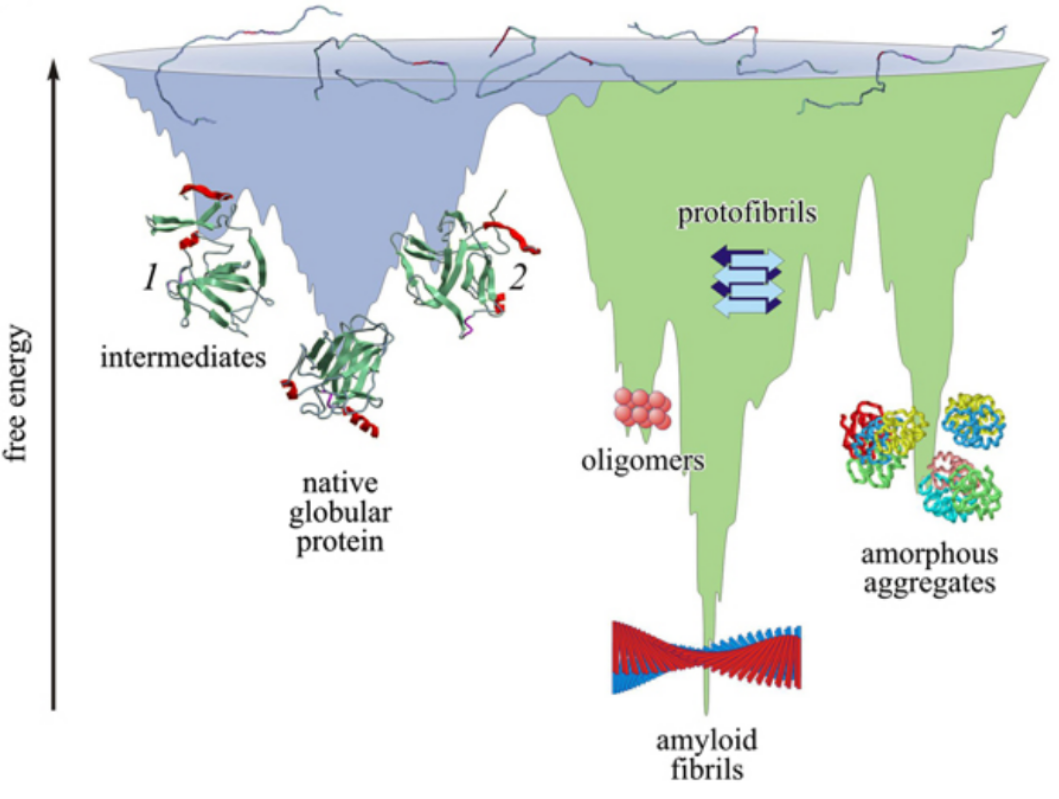
\includegraphics[width=0.7\textwidth]{img/globularEnLandscape.png} 
% \centering
% % 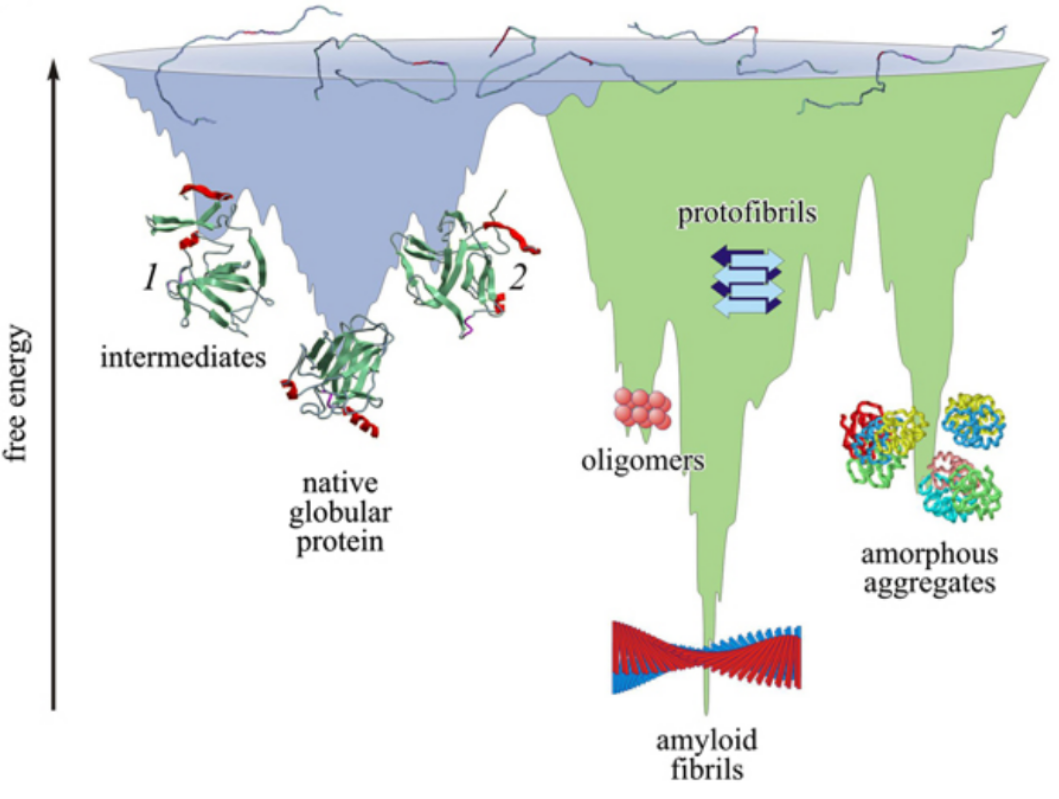
\includegraphics[width=0.7\textwidth]{img/globularEnLandscape.png} 
% \caption{Perfil energetico de los estados de un polipeptido con estructura nativa globular. Figura extraida de \cite{turoverov2010protein}}
% \label{globularFullEnLandscape}
% \end{subfigure}
% 
% \begin{subfigure}[ht]{\linewidth}
% \centering
% 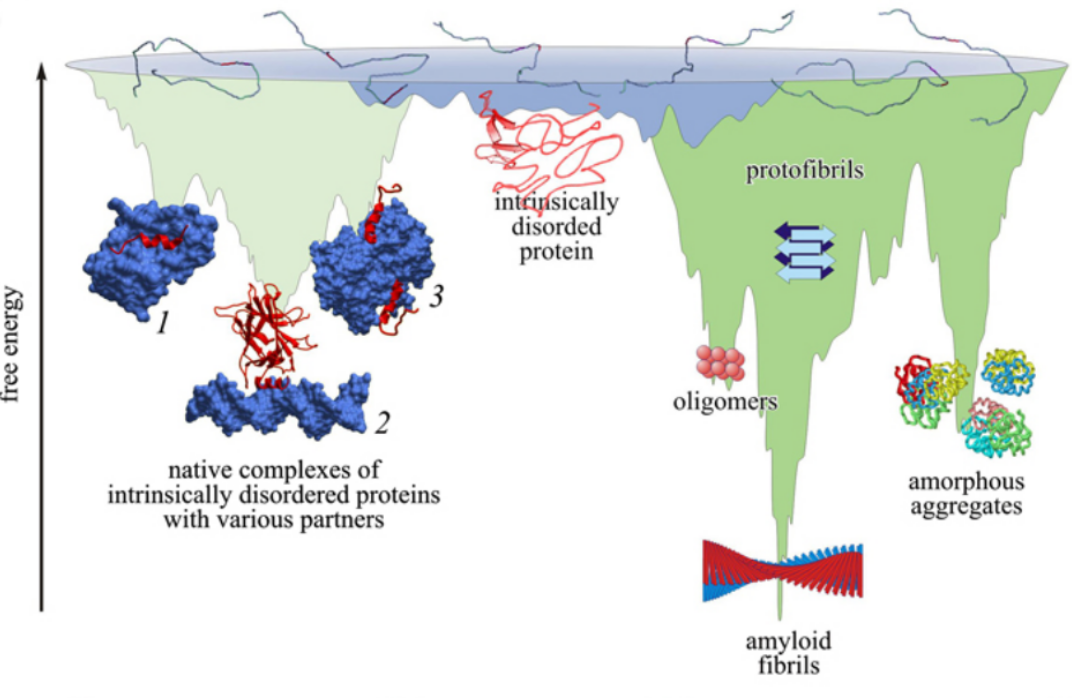
\includegraphics[width=0.7\textwidth]{img/idpEnLandscape.png} 
% \caption{Perfil energetico de los estados de un polipeptido con estructura nativa desordenada. Figura extraida de \cite{turoverov2010protein}}
% \label{idpFullEnLandscape}
% \end{subfigure}
%  \caption{Full energy landscape}
%  \label{fullEnLandscape}
% \end{figure}
% 
% 
% 
% 
% Como se ve en la fig.\ref{fullEnLandscape}\textbf{(a)}, en condiciones normales, donde los proteínas se mantienen en sus estados plegados, 
% la estabilidad de estos estados los mantiene separados mediante barreras cinéticas relativamente altas de la formación de agregados(que se muestran considerablemente mas estables).
% Esto no es tan determinante para intermediarios del plegamiento(estados 1 y 2 en fig. \ref{fullEnLandscape}\textbf{(a)}) y para las conformaciones desplegadas(fig. \ref{fullEnLandscape}\textbf{(b)}), 
% donde las barreras energéticas pueden no ser determinantes en el mantenimiento de los estados nativos en solución.
% Teniendo en cuenta que, como vimos antes, existe una gran diversidad de estados conformacionales en la célula,que el estado totalmente ordenado es, quizás, solo una excepción, 
% y además se sabe que los agregados pueden provocar un gran daño biológico,
% es esperable que los sistemas biológicos hayan evolucionado distintos mecanismos para mantener la homeostasis de los estados nativos monoméricos.
% 







% PROPIEDADES SECUENCIALES
A pesar de esta arquitectura claramente definida de las fibrillas amiloides, las proteínas que forman estos agregados son muy diversas, con muy poca similitud entre sus secuencias.
% o sus conformaciones monoméricas en solución.
Lo que es más relevante, estudios con diversos péptidos y proteínas (no relacionados con aquellos encontrados como causantes de la amiloidosis sistémica) muestran que todos son capaces de formar, 
bajo las condiciones apropiadas, agregados con las características de las fibrillas amiloides.
Estos estudios experimentales, junto con una gran variedad de analisis computacionales, llevan a pensar que la estructura amiloide puede ser adoptada por cualquier cadena polipeptídica y, por lo tanto, 
esta habilidad para reordenar la conformación monomérica y agregarse para formar la estructura amiloide característica puede ser una propiedad intrínseca de las proteínas\cite{fandrich2002behaviour}.
El estado estructural amiloide parece ser, entonces, un estado generico de las proteinas.

Sin  embargo, la tendencia a formar este tipo de fibrillas amiloides si es un proceso que depende específicamente de la secuencia, y algunos detalles estructurales a nivel atómico, 
así como la estabilidad relativa del estado amiloide, pueden ser también características fuertemente dependientes de la secuencia. %REFERENCIAS????  
Por lo tanto, la tendencia a formar estos estados agregados puede variar ampliamente entre distintas proteínas, la pregunta clave es ¿cómo influye la secuencia(o composición) de aminoácidos sobre esta tendencia?
La respuesta a esto es importante no sólo para entender los estados de agregación y sus mecanismos de formación, sino también para otros aspectos como 
la producción biotecnológica de proteínas, o el diseño racional de cadenas polipeptídicas funcionales, donde se desea evitar la formación de agregados al (sobre)expresar las proteínas.
Estos conocimientos sirven también como base para el desarrollo de herramientas bioinformáticas que permitan detectar la tendencia a formación de agregados a partir de una secuencia.

% DEPENDENCIA CON LA COMPOSICION
Se sabe que las interacciones hidrofóbicas son esenciales para la compactación de la estructura lineal de un polipéptido.
Se podría esperar, entonces, que un incremento en el contenido de residuos hidrofóbicos pueda aumentar la tendencia a la agregación de una secuencia, mientras que un incremento en la carga neta impida esta agregación. 
Además de estas propiedades fisicoquimicas, dadas las características estructurales recién descritas para las fibrillas amiloides, con un alto contenido de hojas-$\beta$, 
es razonable pensar que las secuencias que tienen una tendencia intrínseca a adoptar conformaciones de hoja-$\beta$ en su estructura secundaria probablemente tendrán, también, cierta tendencia a la formación de estos agregados.  
% En \cite{chiti2003rationalization} se estudian todas estas propiedades secuenciales mediante mutaciones sistemáticas sobre polipéptidos, concluyendo 
% que la estructura primaria de un polipéptido cumple un papel muy importante en la tendencia a formar depósitos insolubles.


% DEPENDENCIA CON SEGMENTOS DE SECUENCIA
La composición secuencial parece tener un papel importante en la tendencia a la agregación, sin embargo, la combinación lineal de estas propiedades a lo largo de la estructura
primaria puede tener un impacto aún mayor, es decir, no todas las secuencias de polipéptidos con la misma composición tienen la misma tendencia a la agregación.
En \cite{ventura2004short} se demuestran la existencia de ciertos tramos cortos en la secuencia que promueven la agregación en estructuras amiloides.
Estos tramos cortos, llamados generamente regiones propensas a la agregacion(o APRs) se distinguen por tener composiciónes características de residuos, ricas en residuos hidrofóbicos.
% The analysis of the structural models for some amyloids also allow to rationalize the reason why APRs direct the formation of amyloid-like structures, since the cross-$\beta$ arrangement in the core of
% amyloid fibrils does only strictly require the minimum participation of a single $\beta$-strand per molecule, and the rest of the polypeptide may remain exposed to the
% solvent even when “attached” along the fibril.

% ESTO DE LAS REGIONES PEQUEÑAS LO TENGO QUE PONER PORQUE ES LA BASE DE ALGUNOS METODOS QUE DESPUES USAMOS
Además del análisis secuencial, existen otras evidencias a favor de la hipótesis que algunas regiones pequeñas de las proteínas son responsables principales de la formación de fibrillas amiloides. 
Por ejemplo, la mayoría de las IDPs no experimentan agregación \textit{in-vivo}\cite{linding2004comparative} lo que indica que, si bien la conformación no-plegada es necesaria, no es condición suficiente 
para promover el proceso de agregación.
Por lo tanto, deberían existir patrones secuenciales distinguibles que, una vez expuestos(salen del núcleo hidrofóbico de la estructura plegada), son mas propensos a la agregación que otros.  

El hecho que en la naturaleza las IDRs/IDPs no sean necesariamente propensas a la agregación implica, entonces, que sus secuencias han evolucionado para mantener el nivel de solubilidad necesaria que es requerido para 
realizar correctamente las funciones asociadas, por ejemplo, a través de extensas regiones de aminoácidos con grupos polares y altamente cargados que desestabilizan las asociaciones intermoleculares.
Hay que destacar, sin embargo, que existen barreras cinéticas que ayudan a los sistemas biológicos a mantener tanto las IDRs/IDPs como las proteínas plegadas en solución, evitando la formación de agregados no-funcionales 
y manteniendo la homeostasis de los estados proteícos.

% FACTORES EXTERNOS QUE AFECTAN LA AGREGACION
Además de las propiedades que se analizaron sobre la secuencia primaria, es importante destacar factores externos a la secuencia que pueden afectar la formación de agregados.
Los determinantes extrínsecos mas relevantes son el pH y la fuerza iónica de la solución, junto con la temperatura del sistema.
Estas variables pueden afectar tanto la cinética como las propiedades termodinámicas de los diferentes estados e intercambios entre estos.
Estas propiedades afectan a todos los estados posibles aunque en este caso los mencionamos en el contexto de proceso de agregación.





% ACTIVIDADES
Los agregados proteícos estan generalmente asociados con condiciones anormales donde se pierde la capacidad de mantener las proteínas en sus estados nativos correspondientes(pérdida de homeostasis proteica) y, por lo tanto, 
se pierda la capacidad de estas para realizar sus actividades biológicas(al menos de forma correcta) con las obvias consecuencias negativas para el sistema. 
En particular las fibrillas amiloides fueron descubiertas en el contexto de una enfermedad sistémica y se cree que están asociadas a una gran cantidad de enfermedades, sin embargo,
han sido aprovechadas por distintos sistemas biológicos y pueden encontrarse versiones funcionales de estos agregados en distintos organismos\cite{fowler2007functional}.





% % FUNCTIONAL AMYLOIDS
% Amyloids are not only associated with disease-related proteins.
% Nature also exploits the structural and mechanical properties
% of amyloids to regulate biological functions 13 . For example, in
% bacteria amyloids such as curli promote biofilm formation and
% host invasion, and chaplins in bacteria and hydrophobins in yeast
% act as regulators of surface tension of water. Insects and fish
% use chorion amyloid as a component of eggshell, and spiders
% use spidroins in spider silk. Humans possess at least one func-
% tional amyloid protein: Pmel17 is used as a structural scaffold
% in melanin synthesis. The strength and flexibility of amyloids
% have attracted attention for their use as biomaterials. However,
% it remains to be understood how functional amyloids avoid the
% cytotoxic effects observed in disease amyloids. In part, functional
% amyloids are regulated by chaperones and proteases. But it is
% also becoming evident that sequence composition modulates
% critical biophysical parameters determining kinetics of assembly
% or mechanical strength.






% Las fibras amiloides se consideran que estan asociadas to more than 40 human pathologies, esto generó un gran interés en estudiar sus propiedades, 
% las formas detectar secuencias con tendencia a formarse y las formas de prevenir su formación in vivo.


% Since all fibrils independent of the original structure of the given amyloidogenic protein have a common cross-b structure, considerable conformational rearrangements have to occur prior to fibrillation. 
% Such changes cannot happen in a native protein, due to its stable and rigid tertiary structure. Thus, protein destabilization favoring partial unfolding and culminating in the formation of a partially unfolded conformation is required. 
% Presumably, such a partially unfolded conformation favors reciprocal and specific intermolecular interactions, including electrostatic attraction, hydrogen bonding and hydrophobic contacts, which are necessary for oligomerization and fibrillation
% Obviously, this model does take into account a class of natively unfolded proteins, as they are devoid of rigid tertiary structure in their native state.

% Data have been reported indicating that the first critical step in protein fibrillogenesis is the partial unfolding of the protein. 
% Due to structural fluctuations (conformational breathing) the structure of a globular protein under physiological conditions represents a mixture of tightly folded and multiple partially unfolded conformations, 
% with great prevalence of the former. 
% Most mutations associated with accelerated fibrillation and protein deposition diseases have been shown to destabilize the native structure, increasing the steady-state concentration of partially folded conformers

% En la mayoria de las proteinas, excepto las mas pequeñas, el 'unfolding' que ocurre en condiciones fisiologicas no lleva a una estructura totalmente desplegada sino que la proteina adquiere una estructura semi-estable parcialmente collapsada,
% donde las interacciones no son las mismas que en el estado nativo estructurado, estas son caracteristicas propias de los intermediarios del plegamiento.

% The energy landscape model suggests that some folding intermediates might have structural elements not present in the final folded state(en el estado final pueden estar metidas en el centro hidrofobico).
% The appearance of such misfolded intermediates might initiate protein oligomerization or aggregation.

% La formacion de estos intermediarios es importante porque generalmente son mucho mas solubles que si se formaran conformaciones altamente desplegadas. 
% Esta solubilidad permite alcanzar las concentraciones requeridas para la nucleacion propia de la formacion de amyloids(y de agregados en general????)

% Detailed structural analysis of early fibrillation events in several proteins has demonstrated that the amyloidogenic conformation is only slightly folded and shares many structural properties with the premolten globule state.

% This picture enables us to speculate on the origins of the amyloid diseases from the point of view of the physico-chemical properties of the protein molecules. 
% If the stability or cooperativity of the native state of a protein is reduced, for example by a mutation, the population of non-native states will increase.
% This rise will increase the probability of aggregation, as the concentration of polypeptide chains with at least partial exposure to the external environment will be greater. 


% La ocurrencia o no de la formación de agregados dependerá, entonces, de la tendencia intrínseca que posee la secuencia, de la concentración de proteínas y del proceso de agregación.
% Sin embargo, a pesar de la diversidad de estudios al respecto, no se tiene aún conocimiento del mecanismo molecular subyacente a la transformación de proteínas solubles en agregados amiloides.
% % Despite active research, a detailed understanding of the molecular principles underlying the transformation of soluble proteins into amyloid aggregates is still lacking
% % Whether or not aggregation does occur will depend on the concentration of protein molecules, the intrinsic propensity for a given sequence to aggregate when unfolded, and on the rate of the aggregation process. 
% Se ha encontrado que la formacion de fibrillas amiloides puede ser generado utilizando un nucleo estructural como en los procesos de cristalización.
% % The fact that formation of ordered amyloid fibrils can be seeded, like the well-studied processes of crystallization and gelation,
% Esto parece indicar que, una vez iniciado el proceso de agregación, este avanza muy rapidamente en la acumulación y expansión.
% % means that once the aggregation process is initiated it often proceeds very much more rapidly.

% In the absence of seeding there can be long 'lag' phases before aggregation occurs . 
% This lag can be thought of as arising because the growth of a fibril cannot occur until a 'nucleus' of a small number of aggregated molecules is formed. 
% Such a nucleus can be formed by the local fluctuations in concentration that occur in solution as a result of random molecular motion. 
% When such fluctuations result in a local concentration of molecules above a critical value, the molecules associate with one other to form a species that is suficiently 
% large to have intrinsic stability, and hence to grow in size by interacting with other molecules in the solution. The act
% of seeding provides such nuclei to the solution and hence reduces or abolishes the lag phase
% 
% The proposal that amyloid fibrils are a generic structure of polypeptide chains (lo que los hace genericos, que se desarrollo antes) coincide con este modelo de formación.







% 
% The prion protein, for example, is
% thought to undergo a conformational transition
% from a normal cellular form containing a prepon-
% derance of helical secondary structure to a plaque-
% forming conformer containing a greater proportion
% of b-sheet (Pan et al., 1993). Structure determination
% of fragments of the prion protein (Riek et al., 1996;
% James et al., 1997) revealed that  aprox.100 residues at
% the C terminus are folded into a largely helical
% domain. Somewhat surprisingly, NMR studies of
% the full-length protein (aprox200 residues) indicated
% that the N-terminal half of the protein is completely
% unfolded under normal solution conditions (Donne
% et al., 1997). Partial folding of a local region contain-
% ing four octapeptide repeats occurs in the presence
% of Cu(II) ions (Viles et al., 1999) and may give a clue
% as to the overall physiological function of the prion
% protein, which is at present unknown. If this protein
% functions as a copper storage or transport protein,
% the extreme  ̄flexibility of the N terminus is probably
% of functional signi®cance, as the membrane-
% anchored protein picks up copper ions from the
% extracellular fluid.





























\subsubsection{Continuo resultante de estructuras, secuencias y actividades}

Al estudiar las propiedades conformacionales de las proteínas intentamos clasificar los conocimientos en distintos elementos estructurales(proteínas globulares, intrínsecamente desordenadas, etc), esto sirve como modelo para
entender y predecir las propiedades de interé(conformacionales y funcionales principalmente).
La realidad es que, como se dijo en la primera sección de este capítulo, la ocurrencia de proteínas está ajustada a los requerimientos del sistema y al mecanismo evolutivo subyacente, por lo tanto, 
incluso si tratamos de agruparlas en clases distintas, el perfil de muchas propiedades asociadas a las proteínas muestran un perfil que es mejor descrito mediante un continuo de posibilidades.

Ejemplo de esto es el perfil de propiedades conformacionales encontrados en las proteínas. 
A pesar que intentamos distinguir perfiles conformacionales con estructuras tridimensionales definidas(y propiedades dinámicas reducidas), de aquellas que no adoptaban una estructura ordenada, 
el perfil conformacional real que se observa en el proteoma forma un continuo estructural similar al que se ve en la figura \ref{conformationContinuum}.
El extremo izquierdo representa el perfil de las proteinas completamente plegadas. 
En \cite{gall2007intrinsic} se ve que, incluso en la PDB donde las estructuras almacenadas están sesgadas hacia el perfil de proteínas plegadas(porque son las más simples para cristalizar), las conformaciones totalmente ordenadas son 
poco abundantes y que la mayoría de las estructuras posee al menos un segmento desordenado.
Este y otros estudios parecen indicar que el comportamiento de las proteinas totalmente plegadas es la excepción más que la regla, y que la mayoria de las secuencias tienen regiones desordenadas, por lo tanto las estructuras encontradas 
en el proteoma se expanden hacia la derecha del gráfico hasta llegar a un perfil conformacional que no muestra nivel de ordenación estructural a lo largo de su secuencia.


\begin{figure}[htbp]
\centering
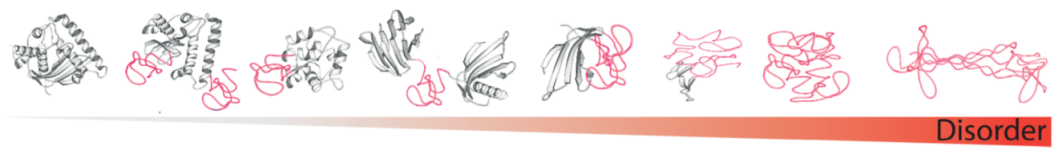
\includegraphics[width=1.0\textwidth]{img/conformationContinuum.png} 
\caption{ Continuo estructural: Los segmentos desordenados pueden comprender solo un pequeño conjunto de aminoácidos dentro de las proteínas u ocupar grandes segmentos de ésta, resultando en un
perfil similar al que se ve en la figura. De izq. a derecha: estructura totalmente ordenada; extremos N y C terminales desordenados; región linker desordenada uniendo dominios globulares; loop desordenado;
dominio completamente desordenado; proteína desordenada con elementos estructurales residuales; proteína desordenada sin elementos estructurales definidos pero con conformación colapsada; proteína totalmente desordenada.
}
\label{conformationContinuum}
\end{figure}






% SACO TODA LA PARTE DE PERFIL ENERGETICO
% 
% DIFERENCIAS EN EL PERFIL DE ENERGIA LIBRE
% Todo lo descrito previamente acerca de proteínas plegadas, sus diferencias con el perfil de las IDRs/IDPs, y la estabilidad de los distintas conformaciones del ensamble, 
% puede entenderse mejor si se analizan las superficies de energía libre asociadas. 
% En la figura \ref{idp-folded-EnergyLandscape} se ven ejemplos de estos paisajes energéticos para tres ejemplos representativos de todo el continuo de conformaciones vistas.
% 
% El gráfico que se ve en la figura \ref{idp-folded-EnergyLandscape}\textbf{(a)} muestra el perfil de energía libre frente a los cambios conformacionales asociados para una proteína plegada.
% El perfil con la forma similar a un embudo, característico de este tipo de proteínas, representa lo que se describió previamente sobre éstas, a través del plegamiento alcanzan una estructura ``única'' que 
% representa el mínimo global de energía. 
% Como detallamos, esta estructura única representa en realidad un ensamble de conformaciones con muy pocas variaciones, capaz de ser representado por una estructura promedio.
% Diversos estudios sobre el proceso de plegamiento resultaron en una gran diversidad de teorías sobre los detalles de este paisaje energético y como se relaciona con el proceso de plegamiento.
% Sin embargo, lo mas relevante se obtiene de observar la forma en que se ubican los mínimos de energía y la amplitud de éstos, lo que nos dará una idea del ensamble real que encontraremos en condiciones fisiológicas.
% % Folded proteins have a "funnel-shaped" global free energy minimum, where the lowest energy state corresponds to the 11native structure, and the width of the unique global energy minimum
% % determines the conformational entropy of the native state.
% 
% A medida que nos movemos hacia la derecha en el continuo de conformaciones posibles de la figura \ref{conformationContinuum}, los segmentos desordenados 
% modifican el perfil energético aplanando la superficie en el mínimo global de energía. 
% Este cambio(graficado en la figura \ref{idp-folded-EnergyLandscape}\textbf{(c)}) representa la existencia de nuevas estructuras con una diferencia conformacional considerable con respecto al resto de las estructuras del ensamble, 
% pero que están separadas entre si por barreras energéticas pequeñas. 
% 
% El perfil energético continua aplanándose a medida que aumentan las regiones desordenadas de la proteína.
% En la figura \ref{idp-folded-EnergyLandscape}\textbf{(b)} se ve el perfil 
% correspondiente a una proteína con una conformación completamente desordenada. 
% 
% \begin{figure}[h]
% \centering
% 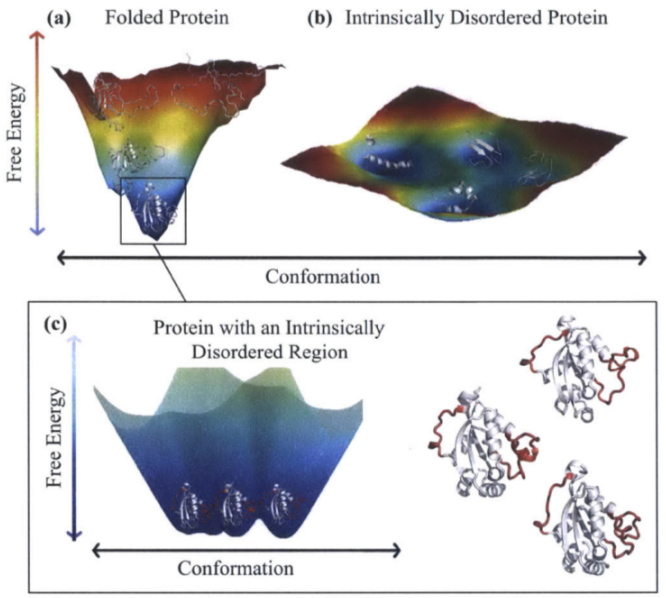
\includegraphics[width=0.7\textwidth]{img/idp-folded-EnLandscape.png} 
% \caption{Diferencias en el paisaje energético entre polipéptidos que adquiren estructuras plegadas, IDRs e IDPs }
% \label{idp-folded-EnergyLandscape}
% \end{figure}










% DIFERENCIAS Y SIMILITUDES ENTRE SLiMs, MoREs e IDD
% 
Algo similar ocurre con los elementos funcionales emergentes de la secuencia.
% A lo largo de las secciones previas vimos diferentes elementos funcionales que, mediante clasificaciones, 
Por ejemplo, como vimos, hay diferencias conceptuales entre los elementos definidos como motivos secuenciales y los MoREs. 
Sin embargo, también existen varias propiedades en común incluyendo la tendencia intrínseca al desorden, ser propensos a experimentar transiciones a estructuras ordenadas y a promover la formación de complejos. 
% Although there are differences in the definitions of linear motifs and MoRFs, they share many common features 72,163 including a tendency to undergo disorder-to-order transition (all
% MoRFs by definition and aprox. 60\% of LMs 48 ), an enrichment in IDRs (MoRFs by definition and aprox. 80\% of LMs are in IDRs 48,72 ), and a tendency to promote complex formation.
Varios estudios sugieren, entonces, que existen un gran solapamiento entre lo que normalmente definimos como motivos lineales y MoREs\cite{fuxreiter2007local,meszaros2012disordered}.
% Yet, interestingly, recent analysis suggests that linear motifs (LMs) (thus not differentiating between ELMs and SLiMs) show high overlap with MoRFs 
Dependiendo si la idea es definida/estudiada desde un punto de vista estructural o secuencial, entonces, un motivo lineal puede ser también identificado como un MoRE o PSE.
Más allá de esto, a pesar de tener una longitud (al parecer) bastante mayor, los IDDs también poseen un solapamiento significativo con MoREs y motivos lineales.
% intrinsically disordered domains (IDDs) can also have significant overlap with MoRFs and linear motifs
Estos resultados parecen indicar que estos elementos funcionales que identificamos con propiedades diferentes pertenecen a estados de un mismo continuo de mecanismos de unión que pueden encontrarse en IDPs.
% The overlap between linear motifs and MoRFs
% especially, but also IDDs, suggests that these functional features
% are different states in the same continuum of binding
% mechanisms involving disordered regions.

% Different concepts regarding short recognition elements have
% been extensively discussed in the literature. Indeed,
% depending
% on whether the idea is approached from a structural point of view
% or defined at the sequence level, a short motif could be denoted
% as a “molecular recognition element” (MoRE)/“molecular
% recognition feature” (MoRF) , a PSE, or “linear motif” (LM),
% respectively (LM is also denoted as “eukaryotic linear motif”
% (ELM) or “short linear motif” (SLiM)).


% ESTO ES LO MISMO, LO COMENTÉ PERO SE PUEDE RESCATAR ALGO
% Whereas LMs have been identified as short sequence motifs critical in recognition functions, primary contact sites, preformed structural elements and molecular recognition elments/features 
% have been approached from the direction of protein disorder, emphasizing recognition segments embedded in such regions. U
% nity of these concepts is underlined by the key role of a few specificity determinants in all these recognition elements, and also by their local preferences 
% for undergoing disorder-to-order transition upon molecular recognition, which might already
% be manifested prior to binding. 
% Apart from a minority of the cases when LMs are constituted of segments of ordered domains, these different concepts of short recognition elements express the same underlying physical and
% functional principles that provide a probably widespread solution to the dynamic control of protein-protein interaction networks.
% 




   
       
       
       

       
%     1.3.1. Ingeniería de proteínas
%         1.3.1.1. Ingeniería de proteínas modulares (a.k.a. quiméricas) (Qué es, 1 página)
%         1.3.1.2. Ejemplos (1 página y 1 figura)
%     1.3.2. Ingeniería de linkers.
%         1.3.2.1. Diseño positivo (propiedades deseadas, 1 página, 1 figura)
%             1.3.2.1.1. Propiedades conformacionales
%             1.3.2.1.2. Carga
%         1.3.2.2. Diseño negativo (propiedades no deseadas, 2 páginas y 1 figura)
%             1.3.2.1.1. Propiedades conformacionales
%             1.3.2.1.2. Propiedades espectroscópicas
%             1.3.2.1.3. Actividades biológicas
%             1.3.2.1.4. Carga metabólica
%         1.3.2.3. Linkers naturales
%             1.3.2.3.1 Características (1 página y 1 figura)
%             1.3.2.3.2 Uso en ingeniería de proteínas (ventajas y desventajas, 1 página)
%         1.3.2.4. Diseño racional
%             1.3.2.4.1 Diseños y conceptos comunes (1 página y 1 figura)
%             1.3.2.4.2 Algoritmos existentes (cómo funcionan, ventajas y desventajas, 2 páginas y 2 figuras)
%             
       
\section{Ingeniería de proteínas}\label{proteinEngineering}
\subsection{Ingeniería de proteínas modulares}    

Como producto de los avances logrados en las tecnologías asociadas al ADN recombinante, se ha desarrollado una nueva generación de proteínas compuestas por la integración
de diferentes módulos secuenciales.

La idea de armar proteínas a partir de la unión de módulos no es algo nuevo, sino que sigue la lógica presentada previamente de que las proteínas naturales son usualmente modulares. 
Es decir, se está simulando el proceso evolutivo natural que desarrolla nuevas proteínas mediante la combinación de dominios preexistentes.

La utilización de la técnica de ADN recombinante para construir nuevas proteínas abre toda una gama de posibilidades que van desde inserción de pequeñas secuencias en extremos de proteína naturales, 
con el fin de poder identificarlas o separarlas, hasta el diseño de construcciones proteicas que buscan obtener nuevas funcionalidades o propiedades diferentes.
% construidas mediante la combinación de distintos dominios.
% En los casos más simples el proceso puede ser ...
% En el caso de nuevos diseños, donde se busca combinar módulos para dar nuevas funcionalidades o hacerlas más eficientes, el proceso experimental puede ser mas complejo.

% s primeros ejemplos de construcciones artificiales probablemente sean la inserción de epítopes o tags(pequeñas secuencias?) en los extremos de alguna proteína para poder localizarlas y/o separarlas.
% en solución o en el entorno celular.
% Más adelante se desarrollaron nuevas construcciones combinando unidades estructurales y/o funcionales en una sola molécula. 
% Esta fusión de dos o más dominios abre toda una gama de posibilidades para construir proteínas con nuevas o mejores funcionalidades.
% 

% Las distintas bases de datos permiten obtener, entonces, una gran cantidad de módulos estructurales y funcionales y gran parte del diseño de proteínas quiméricas 
% se basa en utilizar estos conocimientos y anotaciones para crear nuevas proteínas con estructuras/funciones/propiedades combinadas.

En estos últimos casos, la implementación del proceso experimental suele ser más complejo, requiriendo varios aspectos de diseño a considerar, los 
los cuales no siempre son totalmente independientes entre si. 
% requiriendo un diseño   o un proceso iterativo.
Por un lado está el proceso de diseño/construcción de la nueva proteína.
Por otro están los aspectos asociados con la técnica de ADN recombinante y expresión de proteinas heterólogas. 
En el gráfico \ref{esquemaProcesoFusion} se representan los pasos generales que pueden formar parte de este proceso.

\begin{figure}[htbp]
\centering
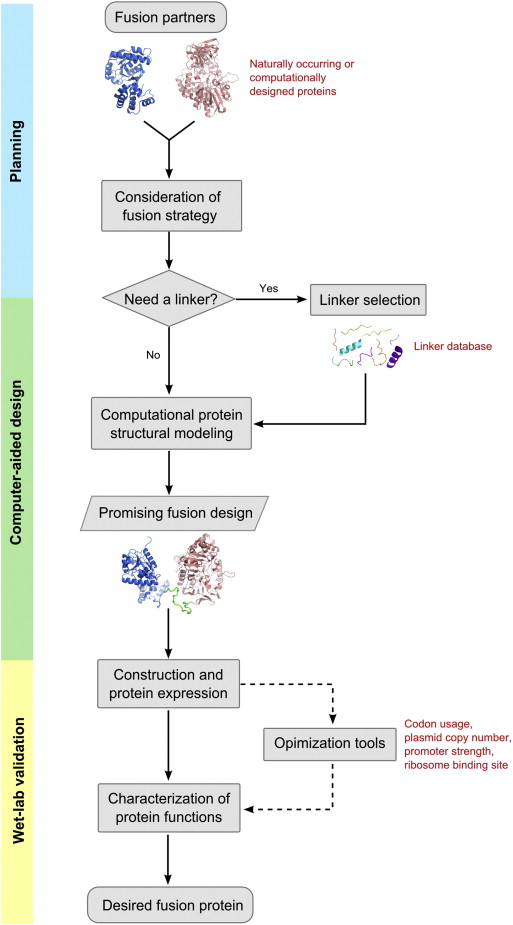
\includegraphics[width=0.7\textwidth]{img/esquemaProcesoFusion.jpg} 
\caption{Figura obtenida de \cite{yu2015synthetic}}
\label{esquemaProcesoFusion}
\end{figure}

La construcción de la proteína de fusión(quimérica) requiere, por su parte, de dos elementos indispensables: 
los dominios o proteínas a fusionar, y la secuencia linker que los va a unir.
La elección de los dominios/proteínas está fuertemente ligada al producto final que se desea obtener y, normalmente, es una decisión directa alrededor de la cual se diseña el resto del experimento.
Por otro lado, la selección de un linker adecuado para unir los dominios/proteinas de acuerdo al objetivo que se busca puede ser un paso complicado y es generalmente ignorado cuando se piensa en el diseño de una proteína quimérica.
La unión directa de los dominios/proteínas o el uso de un linker inadecuado puede resultar en resultados indeseables, por ej. puede restringirse la capacidad de plegado de algun dominio globular, 
bajar el rendimiento de la proteína resultante o disminuir en la actividad biológica de alguno de los módulos.
La correcta selección, o mejor aún, el diseño racional de las secuencias linker para unir los módulos es un aspecto importante, aunque poco desarrollado, del diseño de proteínas quiméricas. 
Esta falta de desarrollo en el tema se debe, quizás, a la falta de conocimiento sobre los factores estructurales que gobiernan la flexibilidad entre los dominios, y es un factor claramente 
limitante en el diseño \textit{de-novo} de proteínas quiméricas. 
Los conocimientos relevantes sobre este tema pueden aparecer a partir de la gran cantidad de secuencias que se disponen actualmente, los avances en 
la identificación de dominios y nuevas técnicas para obtener sus propiedades conformacionales a partir de la información secuencial.





% EJEMPLOS

%

% Examples of this approach include green fluores-
% cent protein (GFP) 1 fusion proteins used in cellular localiza-
% tion studies (1), new antibody types such as multivalent
% antibodies and single-chain antibodies (2-7), artificial
% restriction enzymes consisting of zinc-finger and nuclease
% domains (8, 9),





% AGREGAR ALGO DE TECNICAS FRET
\begin{itemize}
 \item Creación de proteinas que combinan funciones de distintos dominios:
Cómo se dijo en la sección anterior, se poseen cada vez mas dominios anotados con una gran cantidad de funciones correspondientes.
La forma mas común de crear proteinas quiméricas es, entonces, fusionar genéticamente dos o más dominios con subfunciones distintas, obteniendo una nueva funcionalidad global para la proteína.
\item Facilitar el estudio de interacciones proteina-proteina\cite{reddy2013linkers}: 
Tradicionamlente el estudio se hace expresando conjuntamente las dos proteinas que conforman el complejo.
Sin embargo, si la afinidad es muy baja, no es tan simple obtener el complejo formado.
La creación de una proteína quimérica que une a los dominios/proteínas que forman el complejo permite mantenerlas unidas mediante un linker.
La flexibilidad de esta secuencia linker debería permitir la correcta formación del complejo y, al estar unidas covalentemente, habrá una posibilidad mucho mayor de interacción.
El aumento en la estabilidad del complejo permite realizar los estudios biofísicos necesarios sobre éste.
% The characterization of protein–protein interactions is often required to gain an understanding of various biological processes. 
% Yet, the study of protein–protein interactions for many complexes is hampered when one or more partners of the complex are unfolded or unstable. 
% Traditionally, this problem has been addressed by the co-expression and/or copurification of both proteins. 
% However, for weakly interacting or unstable complexes, the co-expression and/or co-purification often results in a single pro-
% tein. 
% Protein engineering techniques were another
% option to address unfolded or unstable proteins,
% using a single polypeptide chain chimera to link the
% two binding partners via a flexible amino acid linker
% 13
% . With these chimeric proteins, it was then possible
% to maintain both the intramolecular and intermolec-
% ular protein–protein interactions, 14 and chimeric
% proteins have been used to generate stable, soluble
% binary complexes for structural studies, as well as
% functional dimers.
% Linking binding partners using an artificial
% linker will increase the proximity between the inter-
% acting partners and preserve the natural interaction.
% In cases where the interacting partners are not
% linked, it is possible that the binding partners might
% dissociate due to their low affinity and/or due to the
% crystallization conditions.
\item La unión de fragmentos de anticuerpos a enzimas o proteínas que permitan la detección de la unión es la base de las técnicas inmunoquímicas.
% \item Incrementar la expresión de proteínas.
\item La unión de segmentos de secuencia específica permite la purificación de proteínas a partir del lisado celular. 
% Facilitar la purificación de proteínas.
% Una de las aplicaciones mas interesantes es para ayudar al estudio estructurals de las intereacciones entre proteinas \cite{}.
% -In addition to structural studies of protein–protein interactions \cite{reddy2013linkers}.,
% \item a wide range of applications in the field of biotechnology have employed these fused proteins
% \item to explore protein-based biochemistry, such as to create artificial bifunctional enzymes and as tools for FRET analysis.

% They have also been widely applied for drug targeting, since proteins such as single chain antibodies or ligands for cell surface receptors can 
% specifically target a linked functional protein (e.g. toxin or cytokine) to a specific type of cells
\end{itemize}












\subsection{Ingeniería de secuencias linker}

% EN ESTA  SECCION PONER LA LISTA COMPLETA DE LOS REQUERIMIENTOS POSITIVOS Y NEGATIVOS DE UN LINKER:
% LONGITUD, COMPOSICION, CONFORMACION DESORDENADA INTRINSECA, AUSENCIA DE ESTRUCTURA SECUNDARIA, AUSENCIA DE ELEMENTOS FUNCIONALES

% \subsubsection{Diseño positivo}


A la hora de obtener un linker las propiedades estructurales suelen ser las más criticas. 
Mantener los dominios unidos a la vez que estos actúan como unidades independientes(manteniendo su funcionalidad), permitiendo que se muevan libremente y la posibilidad de cualquier interacción entre ellos.
Esto depende directamente de la longitud y conformación adoptada por la secuencia linker. 
La longitud no suele ser una propiedad determinante, permitiendo un amplio rango de longitudes efectivas siempre que se eviten las secuencias muy cortas que no permiten una separación suficiente, 
o las secuencias extremadamente largas que harían casi inperceptible la unión de los dominios.
% harían muy ineficaz la interacción entre proteínas.

Los requerimientos conformacionales son un poco mas estrictos y pequeños cambios en la estructura pueden limitar la funcionalidad del nuevo diseño.
En primer lugar buscamos que la secuencia adopte una conformación intrínsecamente desordenada, la cual evita que       manteniendo la
Esta conformación intrínsecamente desordenada provee, además, la flexibilidad necesaria para que los dominios se muevan libremente explorando distintas conformaciones globales.
Para las arquitecturas más comunes, compuestas de dominios globulares unidos por linkers, esta flexibilidad es el requerimiento mas importante ya que permite a los distintos dominios interaccionar libremente.

En la figura \ref{conformacionLinker} se muestran como influyen estos requerimientos en la construcción de una proteína quimérica que une dos dominios EBFP y EGFP. 
Los gráficos A,B y E muestran conformaciones globales de la proteína que son posibles gracias a la flexibilidad del linker intrínsecamente desordenado y con una longitud apropiada. 
Las interacciones que permiten estas conformaciones no se pueden obtener cuando se usa una secuencia con estructura de estructura de hélice-$\alpha$ como se ve en las figuras C y D, donde la rigidez de ésta estructura 
hace que las conformaciones globales sean mucho más limitadas.


\begin{figure}[htbp]
\centering
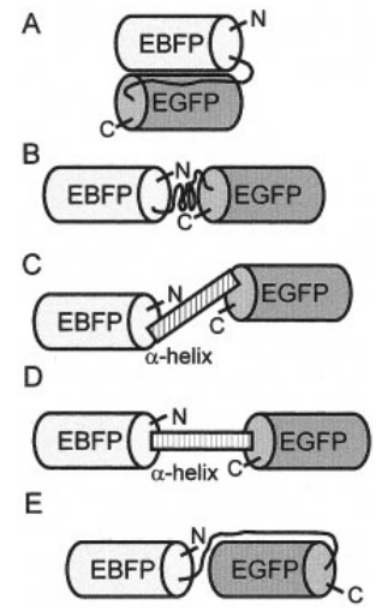
\includegraphics[width=0.3\textwidth]{img/conformacionLinker.png} 
\caption{Figura obtenida de \cite{arai2004conformations}}
\label{conformacionLinker}
\end{figure}


% como vimos antes, el proceso experimental asociado a obtener una proteína quimérica tiene varios pasos, y es importante que la etapa de diseño no se piense en la funcionalidad de la construccion(proteina) 
% de forma aislada sino que se tengan en cuenta las distintas técnicas que pueden/deben utilizarse durante el proceso y en los diferentes contextos donde la proteína se encontrará y donde deberá mantener sus propiedades.

El objetivo de la proteína es poder expresarla en un sistema biológico donde cumplira la función para la cual fue diseñada, por lo tanto es importante que las
propiedades conformacionales del linker se mantengan ante la presencia de otras proteínas o cualquier tipo de ligando.
% MOREs  y Agregacion




% Actividad biologica
La idea del diseño uniendo distintos módulos es que la funcionalidad global se origine exclusivamente a partir de la unión de éstos, por lo tanto la secuencia que los une no debe proveer ninguna funcionalidad adicional, es decir,
debe permanecer inerte ante el entorno en el cual la nueva proteína desarrolla su actividad. 
Las actividades biológicas pueden ser muy variadas pero   
Dado que las propiedades conformacionales  
Entre las actividades biológicas asociadas a estos segmentos están las modificaciones post-traduccionales, unión a ligandos, sitios de clivaje, etc.
Por lo tanto, es importante que la secuencia linker este libre de cualquier funcionalidad asociada a patrones secuenciales lineales. 






% 
% Los requerimientos en el linker no están limitados a la función o actividad de la proteína resultante. 
% Como se vió en la sección anterior, el proceso de 
% 


% COMPOSICION DE AMINOACIDOS: Carga metabolica y propiedades espectroscópicas
% Existen aspectos importantes a la hora de diseñar un linker que podrían parecer obvios, la composición y la longitud del linker son los primeros aspectos a considerar\cite{robinson1998optimizing}.



Por otro lado, la carga de la secuencia puede mediar interacciones en el entorno celular, por ejemplo, al construir proteínas cuya función requiera unirse al DNA es 
requerir que la secuencia linker no tenga residos carga ya que 

Otros requerimientos pueden no aparecer a partir de patrones secuenciales sino de propiedades intrínsecas de cada aminoácido. 
De esta forma, algunos requerimientos están relacionados con la composición secuencial. 
% CARGA METABOLICA
Un ejemplo claro de esto está en poder regular la carga metabólica asociada a la expresión de la secuencia linker. 
Dado que la proteína diseñada deberá ser, finalmente, expresada en algún sistema biológico, y que los distintos aminoácidos que conforman las proteínas tienen distintos costos metabólicos asociados, 
poder controlar la composición(imponiendo una menor frecuencia a aquellos aminoácidos con mas costo metabólico) permitiría incrementar el nivel expresión de la construcción creada.

% propiedades espectroscópicas
En otros casos, el requerimiento está asociado con propiedades fisicoquímicas de algunos aminoácidos. 
Por ejemplo, dado que las dado que las técnicas espectroscópicas se usan de forma rutinaria en el trabajo con proteínas, es deseable que el linker resultante tenga una composición específica tal que no posea aminoácidos que absorban en rango 
del UV, de forma que se elimine cualquier interferencia de la secuencia en este tipo de técnicas.

Otro ejemplo que afecta a la composición está asociada con interacciones iónicas no deseadas. 
Por ejemplo al construir una proteína cuya funcionalidad esté asociada a la unión a DNA, será deseable que la composición final no contenga aminoácidos que puedan encontrarse en estados con carga positiva, debido a que 
la formación de interacciones con la estructura de fosfatos propia del DNA podría interferir en la función de la proteína.

Teniendo en cuenta estos aspectos, una ventaja importante del proceso de diseño es poder definir la composición de la secuencia resultante.


% carga neta
% RESIDUOS CARGADOS
% Una ventaja importante del proceso de diseño es que se pueda definir la carga neta que tendrá la secuencia linker. 
% Este requerimiento puede tener varios fundamentos, principalmente 
Distintas técnicas de laboratorio para identificación y purificación de proteínas se basan en la carga neta de la secuencia.




% Esto se traduce en dos propiedades de la secuencia: que adopte una conformación extendida evitando que los dominios se compacten en el sitio de unión a través del linker, y que no posea una tendencia a adoptar estructuras secundarias, 
% ya que estas podrían reducir el número y tipo de interacciones posibles entre los dominios.


% Es relevante aclarar acá que, si bien los terminos desordenado y flexible pueden solaparse en algun punto, son términos distintos\cite{radivojac2004protein}
% Para una proteína plegada, la flexibilidad refiere a la desviación de las posiciones atómicas con respecto a la estructura promedio en equilibrio.
% Para una region desordenada, la variación en la flexibilidad se refiere a las diferencias en las velocidades de interconversión entre los diferentes estados miembro del ensamble estructural.
% Una variedad de técnicas biofísicas, como por ej. NMR, han sido usadas para estudiar estos conceptos de flexibilidad.

% Análisis de estructuras mediante estas tecnicas muestran que el movimiento en la proteína que provoca los cambios conformacionales puede ocurrir tanto a nivel de residuos como a nivel de estructura secundaria o terciaria. 


% Control of structural flexibility is essential for the proper functioning of a large number of proteins and multiprotein complexes. 
% At the residue level, such flexibility occurs due to local relaxation of peptide bond angles whose cumulative effect may result in large 
% changes in the secondary, tertiary or quaternary structures of protein molecules. 
% Such flexibility, and its absence, most often depends on the nature of interdomain linkages formed by oligopeptides.


% residues or at the secondary, tertiary, or quaternary structural levels. 
% Lactate dehydrogenase, triose-phosphate isomerase, as well as hemoglobin 
% and related proteins are some of the earliest examples of proteins that showed conformational changes with important functional implications.

% 



% 
% 
% 
% 
% La arquitectura típica creada, representada por dominios globulares unidos por secuencias linkers, busca que éstos permitan 
% mantener los dominios separados a la vez que se les da suficiente capacidad para moverse libremente como parte de su funcionalidad. 
% Por lo tanto, la flexibilidad es el requerimiento mas importante, y es deseable que un linker tenga tendencia intrínseca a adoptar una conformación extendida.
% Es importante que, como parte del diseño de la secuencia linker, se asegure que codifique una conformación intrínsecamente desordenada que no posea las características de una estructura colapsada propia de proteínas globulares.
% La conformación extendida le provee la flexibilidad global necesaria, a partir de la rápida interconversión entre la gran cantidad de conformaciones del ensamble con valores de energía similares.
% 
% 
% Un requerimiento asociado 
% Asociado a esto está la idea que una propiedad altamente desfavorable para el linker es que tenga cierta tendencia a adoptar estructuras de hojas-$\beta$ o helice-$\alpha$, ya que los angulos de torsion están limitados al rango
% impuesto por esta estructura, lo que podría también limitar la flexibilidad.
% Como vimos en las secciones previas, 
% aún cuando estas no se encuentren en una conformación plegada compacta típica de proteínas globulares.
% 



% SIGO CON EL EJEMPLO DE FRET QUE HAY MUCHA INFORMACION Y GRAFICOS INTERESANTES
% el ejemplo de FRET permite ejemplificar los requerimientos conformacionales, principalmente de flexibilidad. 
% En este caso, 
% Dado que, la funcionalidad resultante de la proteína quimérica creada depende completamente de la capacidad que 
% 







% % % % % % % ESTO LO PUEDO PASAR A LA PARTE DE LINKERS EMPIRICOS
% 
% % ACA EMPIEZO A HABLAR DE OTROS ASPECTOS NO ESTRUCTURALES
% Sin embargo, la flexibilidad no es todo.  
% Por ej. una opción evidente seria usar linkers de solo Glicina ¿Por qué no usar siempre un linker puramente poli-G, adaptando solamente su longitud?
% Desde los primeros estudios sobre linkers naturales \cite{argos1990investigation} se encontró que las proteinas naturales no usan(seleccionan) este tipo de secuencias.
% Si bien esto no es concluyente para que no se usen, puede darnos un motivo para pensarlo dos veces.
% En primer lugar, un péptido poli-G sería extremadamente inestable y por lo tanto podría actuar como una carga energética, estructural o interferir en procesos de catálisis de los dominios que une, 
% especialmente si tiene una longitud excesiva.
% Se conoce además que el patrón Gly-Gly-X, donde X es un residuo con cadena lateral hidrofóbica, es un sitio target de actividad proteolítica. 
% Por otro lado, una secuencia nucleotídica con alto contenido de Guanina(el codón que codifica para Glicina contiene Guanina en 2 de las 3 posiciones) puede ser difícil de manejar experimentalmente y de expresar para el huésped.
% Como se ve, entonces, existe una gran variedad de aspectos a considerar que exigen distintos requerimientos además de las propiedades conformacionales.
% Por ejemplo, es importante que los linkers should be invulnerable to host proteases, as they are often the targets for degradation. 
% 
% 
% El linker poli-G es sólo un ejemplo. 
% Como vimos en secciones anteriores, distintos elementos funcionales(que actuan principalmente mediante mecanismos de reconocimiento) pueden encontrarse en regiones con distintas propiedades conformacionales. 
% La existencia de estos elementos debe tenerse en cuenta cuando se esta usando la secuencia linker diseñada, y/o su eliminación debe formar parte de la etapa de diseño del linker.
% La longitud del \textit{loop} creado por el linker puede tener un profundo efecto sobre la actividad del linker en una proteína quimérica\cite{nagi1997inverse}.
% Además del ejemplo simple de resistencia proteolítica, las regiones linker también pueden afectar la estabilidad, solubilidad, formación de complejos.
% linker regions can affect the stability, solubility, oligomeric state, and proteolytic resistance ofthe fused protein
% Como se muestra en \cite{robinson1998optimizing}, en algunos casos se tienen efectos importantes variando la longitud y composición de la secuencia
% En base a esto, es esperable que se tengan requerimientos específicos relacionadas con la longitud y la composición. 
% % The stable linkage between functional domains provides many advantages such as a prolonged plasma half-life (e.g. albumin or Fc-fusions). 
% % However, it also has several potential drawbacks including steric hindrance between functional domains, decreased bioactivity, and altered biodistribution and metabolism of the protein moieties due to the interference between domains 
% % In other systems, however, linker regions can affect the stability, solubility, oligomeric state, and proteolytic resistance of the fused proteins
% % Thus, it is important that the length and amino acid composition of a potential linker is optimized in order to preserve the biological activity of the individual proteins in the fused complex.
% 
% 





% \subsubsection{Diseño negativo}




% Además de los analisis sobre las propiedades físicas asociadas a las arquitecturas modulares, el estudio de la diversidad de linkers
% encontrados en la naturaleza puede proveer información importante para entender los requerimientos
% más importantes en el diseño de estas secuencias.


\subsubsection{Linkers naturales}



% 


% El 'descubrimiento' de las regiones/secuencias linkers esta ligado a las teorias de structura-funcion(desarrolladas en la parte de conformacion) que se dieron durante casi 100 años
% En un principio se comenzo a pensar en una estructura rigida asociada a la proteina, luego se fueron revelendo propiedades dinamicas que le permitian cumplir la funcion. 
% Todo esto esta muy asociado a las tecnicas experimentales que se fueron desarrollando.

Como se dijo antes, la modularidad en proteínas naturales es algo muy común y existen muchisimos ejemplos de proteinas multidominio compuestas de dos o mas dominios funcionales unidas por linkers.
Estas secuencias linker sirven, principalmente para mantener unidos los distintos dominios, pero también proveen muchas otras funciones a la proteína como intervenir en las interacciones cooperativas 
entre los dominios o formar parte de la actividad biológoica de la proteína.

El primer estudio realizado sobre secuencias linkers \cite{argos1990investigation} registra la preferencia intrínseca por las conformaciones desplegadas.   
Sin embargo este estudio está bastante desactualizado y los resultados no son representativos ya que se realizó sobre un total de 51 linkers detectados manualmente a partir de 32 proteínas.
En \cite{george2002analysis} se encuentra un análisis más actual sobre un total de 638 proteínas multidominio,  a partir de las cuales se determinaron las regiones linkers(un total de 1280) y dominos utilizando un método automático.

% encuentran los análisis mas detallados donde se estudian las propiedades generales de secuencias linkers naturales

En \cite{chen2013fusion} se revisan los resultados obtenidos en ambos con respecto a diversas propiedades como son longitud, hidrofobicidad, enriquecimiento de ciertos aminoacidos y estructura secundaria adoptada.


% in general, preferable amino acids were polar uncharged or charged
% residues, which constitute approximately 50\% of naturally encoded amino acids. Both
% studies suggested that Pro, Thr, and Gln were the preferable amino acids for natural linkers.

% The preferred linker amino acids observed in the majority of
% the linker sets are Pro, Arg, Phe, Thr, Glu and Gln, in order
% of decreasing preference

Among them, Pro is a unique amino acid with a cyclic side chain which causes a very
restricted conformation [25]. The lack of amide hydrogen on Pro may prevent the formation
of hydrogen bonds with other amino acids, and therefore reduces the interaction between the
linkers and the protein domains.
As a result, the inclusion of Pro residues might increase the
stiffness and structural independence of the linkers.

Proline is unique among protein residues as
it is a cyclic imino acid with no amide hydrogen to donate in
hydrogen bonding. Therefore, it cannot fit into the regular
structure of either $\alpha$-helix or $\beta$-sheet and is a common ``breaker''
of secondary structure.
Proline will introduce some motion into a
helix, that enables a number of different conformations at that
region

Short proline rich sequences are
stiff, with non-interacting connections. As suggested before,
this is the most likely reason why proline is the preferred
linker constituent, particularly in non-helical linkers. It cannot
hydrogen bond to any surrounding amino acids, avoiding
ordered structure formation and contact with the neighbouring
domains.




% PROPIEDADS ESTRUCTURALES

% ESTRUCTURA SECUNDARIA
% Natural linkers adopt various conformations in secondary structure, such as helical, β-strand, coil/bend and turns, to exert their functions.
% the largest proportion of linker residues, 38.3\%,
% adopt the α-helical secondary structure, 13.6\% are in
% β-strands, 8.4\% are in turns and the rest, 37.6\%, are in coil
% or bend secondary structures.


En general, se encontro que los linkers naturales adoptaban principalmente conformaciones desplegadas y tenían estructuras independientes sin interacciones con los dominios adyacentes.
En términos de estructura, por ejemplo, se encontraron tanto linkers flexibles como relativamente rígidos en muchas proteínas.
A través de una mayor rigidez, ciertos linkers pueden ayudar a reducir interacciones no funcionales entre los dominios que unen. 
Por otro lado, una estructura más flexible, como es usual para conformaciones extendidas, provee una mayor flexibilidad y libertad de movimiento a los dominios.


% En \cite{george2002analysis} se esboza una clasificación de los linkers de acuerdo al análisis de su estructura secundaria.
% Se dividen, así, en dos categorías: helicoidales y no helicoidales.
% Los linkers con estructuras de $\alpha$-hélice pueden tener funciones como, por ejemplo, actuar como espaciadores rígidos impidiendo interacciones no funcionales entre los dominios.
% Aunque no sea exhaustiva, esta clasificación permite ver diferencias en los linkers también a nivel de estructura que adquieren, existiendo linkers que, a través de una mayor rigidez, impiden . 




Todas las propiedades analizadas(longitud, composición, hidrofobicidad y estructura secundaria.) resultaron importantes para alcanzar las funciones deseadas.


% AL FINAL DE TODO PONGO ESTOS EJEMPLOS, DEMOSTRANDO QUE LA FUNCIONALIDAD DE LOS LINKERS NO ESTÁ LIMITADA A PROVEER FLEXIBLIDAD Y QUE PUEDEN CUMPLIR OTRAS FUNCIONES

%EJEMPLOS DE PROPIEDADES CONFORMACIONALES
En terminos de flexibilidad, y por lo tanto de propiedades conformacionales en general, los linkers muestran 

en algunos casos la flexibilidad provista por los linkers naturales se origina a nivel de estructura secundaria, y esta limitada a una región corta que funciona como bisagra.
% EJEMPLO!!!!
En otros casos la flexibilidad es ``completa'' y la región del linker es intrínsecamente desordenada\cite{luo2010flexibility}, 
% EJEMPLO !
encontrándose incluso que la funcionalidad de la proteína se pierde cuando se reemplaza por un linker con \cite{hrycyna1998structural}

Ademas, existen linkers que, a pesar de mantener una conformación extendida en solución, pueden plegarse (o fijar una estructura secundaria transitiva) en presencia de ligandos.
Por ejemplo en el caso de ciertas proteínas que se unen a DNA\cite{laity2000dna}
%ESTE ES UN EJEMPLO DE FUNCIONALIDAD 


En algunos casos, las secuencias linker permiten mediar la propagacion eficiente de los efectos originados por la unión de ligandos o modificaciones post-traduccionales en uno de los dominios que conecta(alosterismo).
Un ejemplo es el caso de la miosina del musculo liso, en la cual un dominio que comprende la funcion motora es activado mediante fosforilacion  de una cadena regulatoria unida a este mediante un linker\cite{ikebe1998hinge}.
% OTRO EJEMPLO
% An example is the intramolecular interaction between the Src homology domains (SH2 and SH3) and the catalytic domains of Src family kinases, which results in repression of catalytic
% activity. Repression by the regulatory domain is nullified upon mutation of Trp260 to Ala within the linker separating the SH2 and kinase domain, which proves that the linker plays a crucial role in the coupling of
% the regulatory domains to the catalytic domain



%  ejemplo de la importancia de la secuencia linker en 
% otro ejemplo de funcionalidad esta en  \cite{tsutsumi2012charged}  ...



% CONCLUSIONES
Por lo tanto, a pesar que la flexibilidad es un aspecto que se sabe esta ligado a las secuencias linker en la naturaleza\cite{wriggers2005control}, 
y que estás regiones son generalmente las que permiten los grandes cambios conformacionales en las estructuras de las proteínas, 
estas no son simplemente secuencias que evolucionan hacia conformaciones totalmente flexibles, ya que esto puede no estar directamente ligado al cumplimiento de la función requerida, o no hacerlo de forma eficiente.

De esta forma, las secuencias linker en la naturaleza son una parte mas de las proteínas y sus propiedades conformacionales no pueden definirse como generales, sino que están 
% De esta forma, las propiedades conformacionales de las regiones linkers naturales están usualmente 
asociadas a restricciones funcionales de la proteína global, buscando balancear la flexibilidad requerida 
para que los dominios puedan explorar el ensamble de conformaciones asociado a su funcionalidad, con la rigidez requerida para que no existan interacciones desfavorables entre estos, 
resultando en perfiles muy variados de flexibilidad.

En cada proteina, la secuencia linker puede tener una estructura y una función que haya sido seleccionada para el mecanismo/localización/función de la proteina como un todo, 
y esta función del linker puede no ser solamente la unión covalente de dos dominios. 

Las propiedades funcionales no solo afectan a la conformación sino que abarcan la longitud, composición y propiedades secuenciales puntuales.





% UTILIZACION DE LINKERS NATURALES PARA 
Dado este contexto, el uso de secuencias linkers naturales en el contexto del diesño de proteínas quiméricas debe realizarse con mucho cuidado.
........

% ACÁ PUEDO PONER QUE LOS LINKERS NATURALES TAMBIEN PUEDEN SERVIR COMO BASE PARA UN PROCESO DE INGENIERIA?? O LO PASO A LA PROX. SECCION???









% Los primeros estudios de analisis (estructura y composicion) de secuencias linkers\cite{argos1990investigation} se comenzaron a hacer a partir del analisis estadistico de secuencias que podian ser clasificadas 
% como linkers a partir de las primeras estructuras de proteinas multidominio almacenadas en bases de datos.
% % Estos estudios estaban sesgados por todo el proceso historico de descubrimiento marcado por 
% Los resultados indicaban que la mayoria adquiría una conformación desplegada(tipo \textit{coil}) sin estructura secundaria. 
% % many studies of linker peptides in various protein families have come to the conclusion that linkers lack regular secondary structure (la mayoria se encontraba en estructuraas tipo coil), 
% % they display varying degrees of flexibility to match their particular biological purpose and are rich in Ala, Pro and charged residues
% Asi surgio la idea que los linkers eran secuencias cortas cuya unica funcion era proveer la conexion covalente, lo que estaba de acuerdo con el concepto de hinge-bending.
% Este concepto indicaba que la flexibilidad de estas regiones cortas dentro de un polipéptido permitía el suficiente movimiento a los dominios estructurales.
% % The concept of hinge-bending, whereby the relative flexibility of these short regions of the polypeptide chain allows significant movement of structural domains, gained widespread acceptance in
% % the 1980s and early 1990s, after evidence for conformational transitions in identical or homologous proteins became known.



% A lo largo de los años los conocimientos sobre la composición y propiedades de estas secuencias ha ido cambiando, 
% a medida que mayor cantidad de estructuras se resolvian y mayor conocimiento se obtenia acerca de los dominios que componen 
% las proteinas. Tambien influyeron otras cosas como tecnicas biofisicas que permiten obtener información del ensamble conformacional en solución,
% o algoritmos para automatizar la identificación de los dominios y las secuencias que actúan como linker en una proteina.
% 

% Although the role of linker sequences is likely to be primarily topological, allowing distant parts of the polypeptide chain to interact with diverse partner sequences that might be far apart or close together, 
% linkers and unstructured tail sequences play quite specific roles in a number of systems.








% A FUTURO
Con el incremento del número de estructuras almacenadas en la PDB que ocurrió en los últimos años, sería posible realizar un estudio actualizado de las propiedades de los linkers naturales.
Además, sería interesante extender el número de propiedades analizadas agregando categorías asociadas a función y estructura de la proteína, e identificando la relación entre estas y las propiedades del linker.
% With the rapid increase of the number of protein structures deposited in the PDB database, an updated study of natural linkers could be conducted. 
% In addition to the properties analyzed in previous studies (e.g., amino acid composition, structure classification), 
% it would be interesting to categorize the multi-domain proteins by their functions and structures, and identify the relationship between them and the linker properties


% 
% 
% Based on From George and
% Heringa’s secondary structure analysis, linkers were grouped into two categories: helical and
% non-helical. The $\alpha$-helix was a rigid and stable structure, with intra-segment hydrogen bonds
% and a closely packed backbone [28]. Some $\alpha$-helical conformations form rapidly during
% folding [28], allowing the correct folding of connecting protein domains without non-native
% interactions with the linker. Linkers in an $\alpha$-helix structure might also serve as rigid spacers
% to effectively separate protein domains, and to reduce their unfavorable interactions.
% Therefore, this conformation was commonly adopted by many natural and empirical linkers
% (to be discussed later). On the other hand, without an inherent rigid structure, the non-helical
% linkers tended to be rich in Pro, which could increase the stiffness of the linker as mentioned
% previously [25]. As a result, non-helical linkers with Pro-rich sequence could exhibit
% relatively rigid structures and serve to reduce inter-domain interference.
% 
% 
% 
% Both flexible and relatively rigid peptide linkers are found in many multidomain proteins. 
% Linkers are thought to control favorable and unfavorable interactions between adjacent domains by means of variable softness
% furnished by their primary sequence. Large-scale structural heterogeneity of multidomain proteins
% and their complexes, facilitated by soft peptide linkers, is now seen as the norm rather than the
% exception. Biophysical discoveries as well as computational algorithms and databases have
% reshaped our understanding of the often spectacular biomolecular dynamics enabled by soft linkers.
% Absence of such motion, as in so-called molecular rulers, also has desirable functional effects in
% protein architecture.







% 
% 
% \subsubsection{Molecular rulers}
% These linkers are more defined by their ability to reliably predict and maintain end-to-end distances between attached domains. 
% Such structurally rigid peptides have been conjugated to molecules to serve a metric function.
% These linkers are rich in Proline. 
% Proline is common to many naturally derived interdomain linkers, and structural studies indicate that proline-rich sequences form relatively rigid extended structures to prevent unfavorable interactions between the domains.
% The probable reason why proline is favored over other residues in linking different domains is the inability of proline to donate hydrogen bonds or participate comfortably in any regular secondary structure conformation. This ensures a relatively rigid separation of the domains, thereby preventing unfavorable contacts between them.
% 
% Although short stretches of hard linker sequences are located between functionally relevant regions of protein structure, mutations within such sequences may have no effect on the function.  
% Such linkers are therefore necessary to keep the other amino acid interactions in register, but the nature of the side chain is often unimportant.
% 
% The observed natural tendency to form rigid linkers might also
% be related to avoiding proteolytic cleavage, as linkers are likely
% targets for protease degradation
% 
% Linker
% sequences vary greatly in length and composition, but
% many are rich in polar, uncharged amino acids (such as
% Ser, Thr, Gln and Asn), in the small residues Ala and Gly,
% and in Pro residues. Many of these residues tend to bias
% the polypeptide chain towards the polyproline-II region
% of the RAMACHANDRAN PLOT 27,28 .This means that such
% linkers, although flexible, have a propensity to be highly
% extended. Compositionally biased linker sequences of
% significant length are found mainly in eukaryotic pro-
% teins 1,29 , but short linker sequences of similar composi-
% tion, known as Q-linkers, are also found in a number of
% bacterial regulatory proteins 30 .
% In the absence of their targets, modular proteins
% often behave as ‘beads on a flexible string’, where the
% function of the linker is, primarily, to enable a relatively
% unhindered spatial search by the attached domains 31 .
% However, binding can induce structure formation in
% linkers, which can have significant functional conse-
% quences. For example, the sequence-specific binding of
% CYS HIS ZINC-FINGER PROTEINS to DNA causes the linker to
% fold, cap and thereby stabilize the preceding helix in the
% protein, and to orientate the next zinc finger correctly
% for binding in the major groove of DNA
% 
% 















\subsubsection{Diseño racional}


Con tantos, y tan distintos, requerimientos positivos y negativos, el problema del diseño de linkers puede llegar a ser un tema complejo.
El problema del diseño racional es, entonces, un proceso complicado.
% The general properties of linkers derived from naturally-occurring multi-domain proteins(que se vieron en la seccion anterior) can be considered as the foundation in linker design. 
Las propiedades generales de los linkers naturales encontrados en proteínas multi-dominio pueden considerarse como un primer paso hacia el proceso de diseño.



% PRIMERO HABLAR DE LINKERS USADOS EMPIRICAMENTE 

% Además de la utilización de linkers naturales, una opción común es reutilizar linkers ya utilizados empíricamente, 
La opciones actuales del diseño de linkers se basan, generalmente,  en reutilizar secuencias ya evaluadas empíricamente, buscando la que más se adapte a nuestros requerimientos. 
Muchas de estas secuencias son linkers naturales y otros han sido modificados especificamente en cada caso por procesos de ingeniria.
% Linker engineering, with the aim to control the distance, orientation, and relative motion of two functional domains, will increase in importance with increasing emphasis on the de novo design of multi-domain proteins.
En \cite{chen2013fusion} se hace un análisis de los linkers empíricos más usados para creación de proteínas quiméricas y que pueden encontrarse en literatura, diseñados mediante aproximaciones muy distintas.
A partir de esta recopilación se intenta hacer una clasificación general que resulta en 3 categorias:
linkers flexibles, linkers rígidos, y linkers que pueden experimentar clivaje \textit{in-vivo}. 
Como se puede ver, esta clasificación esta basada, principalmente, en propiedades estructurales/conformacionales. 
Para obtener secuencias que posean otras propiedades de interés deberán analizarse cada uno de los linkers que se detallan en este trabajo.
Los linkers que se encuentran  en la literatura fueron construidos en base a la intuición y la posterior validación experimental.


En el caso de fusiones que requieren linkers flexibles, la mayoría se construye en en base a la intuición utilizando residuos pequeños(polares o no polares) tales como Gly, Ser y Thr,
siendo el linker más común encontrado en la literatura el compuesto por distinto número de repeticiones del motivo $(G_4S_n)$. %PONER REFERENCIAS AL USO DE ESTE.
También se ha utilizado linkers poliglicina($G_n$), en estos casos la sustitución de algunas posiciones por residuos polares (Ser) busca reducir las interacciones no deseadas entre el linker y los dominios que une de forma
tal que no interfieran en la funcionalidad.
Una aproximación de diseño más avanzada se puede ver en \cite{bird1988single}, donde se utilizan residuos Gly y Ser para proveer flexibilidad pero se agregan Glu y Lys para incrementar la solubilidad.
% COMENTAR EL METODO USADO MAS EN DETALLE


% peptide sequences consisting of flexible and hydrophilic residues (arbitrary repeats of glycine and serine residues) are used because they are assumed to form a random coil and do not interact with (the folding of)
% the protein domains
En la mayoría de estos casos, los péptidos con motivos repetidos de Gly y Ser son usados porque se asume que adoptan una conformacion similar a random coil y no interfieren en el plegado y funcionamiento de los dominios que unen,
la funcionalidad provista por estos se evalúa en cada caso en particular.
En \cite{evers2006quantitative} se hace una evaluación de estos linkers tan usados, en el contexto de la unión de dos proteínas fluorescentes, evaluando cuantitativamente las propiedades conformacionales y el efecto de la longitud del linker 
a partir de la transferencia de energía entre estas.


Estos linkers poseen conformaciones desestructuradas (Gly suele considerarse como capaz de romper la estructura ordenada de las hélices), y esta flexibilidad puede, en algunos casos, impedir que se logre una separación 
suficiente entre los dominios (Evers et al., 2006).

As a result, more rigid linkers including polyproline motifs (
Schuler et al., 2005 ) and an all
a-helical linker A(EAAAK)n A(Arai
et al ., 2001) have been developed.




% LINKERS RIGIDOS
% ref 34 = \cite{arai2001design}
% ref 35 = \cite{arai2004conformations}
% 
% An empirical rigid linker with the sequence of A(EAAAK) n A (n = 2-5) was first designed
% by Arai et al. [34, 35]. The linker displayed α-helical conformation, which was stabilized by
% the Glu − -Lys + salt bridges within segments. To test whether they could effectively separate
% the protein domains, these helical linkers were inserted between enhanced blue fluorescent
% protein (EBFP) and enhanced green fluorescent protein (EGFP), and the fluorescent
% resonance energy transfer (FRET) efficiency between EBFP and EGFP was measured [34].
% The FRET efficiency decreased as the length of helical peptides increased, indicating that
% helical linkers can control the distance between domains by changing repetitions of the
% EAAAK motif. Compared to flexible linkers with the same length, the helical linkers
% induced much less FRET efficiency when inserted into EBFP-EGFP fusion proteins,
% suggesting that helical linkers can separate functional domains more effectively.







% PONER LOS EJEMPLOS QUE USAN UNA COMBINACION DE ESTOS LINKERS RIGIDOS Y FLEXIBLES PARA UN DISEÑO DE FRET:
% el linker totalmente flexible permite todo tipo de interacciones entre los dominios, pero
% en este caso lo que se busca es que en la conformacion normal se evite lo mas que se pueda las interacciones entre dominios, ya que estas generan resonancia energetica no deseada(solo se quiere).
% primero: Antibody Detection by Using a FRET-Based Protein Conformational Switch: 
% aca lo que buscan es un linker suficientemente flexible para permitir la interaccion de las dos partes del sensor en su forma no unida al anticuerpo(teniendo asi una alta tasa de emision),
% pero que a la vez permita un 'efficient bridging'(mantenga cierta distancia) como para que, al unirse ambos extremos al anticuerpo, se pierda la interaccion disminuyendo la tasa de emision.
% primero usan un linker super flexible (17 Gly-SerGly repeat), despues prueban uno que incorpora motivos alfa-helice
% El segundo caso donde se usa este nuevo linker es en: a sensor for quantification of macromolecular crowding in living cells
% El linker que terminan usando en ambos es $A(EAAAK)_6A(GSG)_6A(EAAAK)_6A$








% DESPUES EMPIEZO CON DISEÑO RACIONAL

El diseño racional de linkers, sin embargo, está aún en los principios del desarrollo. 


% Although many examples of various types of linkers have been developed in the past, the rational design of linkers for the construction of fusion proteins is still in its infancy. 

En algunos casos se ha 
Existen pocos ejemplos concretos donde se haya utilizado una aproximación racional para el diseño de linkers \cite{arai2001design,arai2004conformations}.

Los estudios detallados de la composición, estructura y función de linkers naturales son un claro punto de inicio.
Con el rápido incremento de los conocimientos sobre la secuencia y estructuras de proteínas, nuevos estudios podrían aportar conocimientos relevantes en esta dirección.
Sin embargo no hay indicios sobre posibles desarrollos orientados a obtener un método sistemático para el diseño racional.  
% Systematic, strategic scientific endeavors are in demand to greatly advance the science of linker design and application.
% Many technology platforms may be investigated in more depth towards understanding the connection between linker composition and structure, and ultimately tie them to linker function.
% The study of linker composition and structure, and the investigation of linker function should go hand in hand when designing a novel linker.
% With the rapid increase of the number of protein structures deposited in the PDB database, an updated study of natural linkers could be conducted.
% The establishment of more databases and searching programs for linkers would be another fruitful direction. 
% As discussed earlier, only two studies have been performed to analyze the characteristics of the linkers in natural multi-domain proteins.
% ESTO ESTA CASI IGUAL EN LA SECCION ANTERIOR

% The extensive studies on the structures of empirical linkers have provided us with useful information for optimal linker design. 
% Ultimately, more searching algorithms for linker databases could be developed, and provide more linker candidates for protein fusion based on user specifications.










% FINALMENTE EXPLICAR LAS APROXIMACIONES RACIONALES QUE ENCONTRE, QUE CONSISTEN BASICAMENTE EN BUSCAR EN BBDD


Los estudios realizados sobre linkers naturales(mencionados en la sección anterior) abrieron la posibilidad de crear bases de datos conteniendo las secuencias encontradas y sus propiedades asociadas.
Asociados a estas bases de datos, se han desarrollado distintos métodos que permiten extraer  ,  que simula un mecanismo de diseño.
% The extensive studies about linkers in natural multi-domain proteins and recombinant fusion proteins fostered the idea of building databases and coming up with linker (designing??) tools 
% to aid the (rational???) design of linkers based on the desired characteristics of fusion proteins.
% Es decir, actualmente la metodologia esta centrada en crear bases de datos de linkers y hacer consultas sobre esta en base a las propiedades que se buscan.

Los resultados del estudio desarrollado en \cite{george2002analysis} son el primer ejemplo de este tipo de metodologías.
% An example of this type of tools was developed during the analysis of a protein dataset to obtain information about linker sequences 
En este trabajo se estudian diversos aspectos asociados a los linkers y se desarrolla una base de datos asociada a un algoritmo de búsqueda que puede ser utilizado mediante un servidor web\cite{linkerdbIBIVU}.
El algoritmo implementado acepta distintos parámetros de búsqueda tales como longitud del linker, accesibilidad del solvente, estructura secundaria adoptada, similitud secuencial con una secuencia input, etc.
% The search algorithm accepts several query types (eg, PDB code, PDB header, linker length, C-alpha extent, solvent accessibility, secondary structure or sequence). 
El programa devuelve las secuencias linker que contienen los criterios solicitados y, además, provee información del contexto en el que se encuentra el linker, con información del ID en PDB, descripciones de la proteína, etc. 
de forma que el usuario pueda inferir otras propiedades del linker que no pueden ser extraídas automáticamente.
% The program can provide the linkers sequences meeting the searching criteria, and also provide other information such as the PDB code and a brief description of the source protein, 
% linker’s position within the source protein, linker length, solvent accessibility, and secondary structure. 
% Users can search for sequences with desired properties, and obtain candidate sequences from natural multi-domain proteins.

Otro ejemplo de búsqueda sobre bases de datos es \url{http://bioinf.modares.ac.ir/software/linda/}

Un ejemplo más reciente de este tipo de aproximación mediante bases de datos da origen a la herramienta LINKER \cite{crasto2000linker,xue2004linker}.
% A more recent example of this type of tool is a program called LINKER 
Al margen de la falta de creatividad en el nombre de la aplicación, esta posee un método de búsqueda que brinda una gran cantidad de opciones al usuario incluyendo aspectos experimentales como la sensibilidad a la actividad de proteasas.
% which searches its database of linker sequences with user-specified inputs (e.g., linker length, protease sensitive sequences to be avoided), and generates an output of several linker sequences that fit the criteria.
En este caso, el centro del método es base de datos conteniendo secuencias loop extraidas de PDB y que son luego levemente procesadas removiento secuencias idénticas, hairpin loops y secuencias de menos de 4 residuos. 
El programa de búsqueda/diseño construido sobre esta base de datos asume que la conformación de loop adoptada por la estructura cristalizada que se encuentra en la PDB dará una conformación extendida 
si se utiliza esta secuencia como linker en una proteína quimérica
Desafortunadamente, el servidor web asociado a este programa no está más disponible.



Una nueva versión de este tipo de soluciones se realizó este año en \cite{liu2015synlinker}. 
La particularidad de esta nuevo programa es que incorpora en su base de datos, no sólo a secuencias linker naturales sino también algunos linkers empíricos extraídos de la literatura, 
que siguen los principios de diseño/construcción que vimos hasta ahora en esta sección.
Una particularidad de esta herramienta es que permite obtener un modelo computacional donde 1 o mas linkers se fusional con estructuras/dominios obtenidos de la pdb. 
Este modelo puede ser usado directamente como input en el próximo paso(siguiendo el esquema de la figura \ref{esquemaProcesoFusion}) donde se pueden evaluar mediante simulaciones de dinámica molecular algunas propiedades conformacioneles de la construccion obtenida.



A pesar que las bases de datos no proveen una solución total al problema de diseño, la construcción de estas y los métodos de búsqueda asociados 
ayuda a la utilización de los conocimientos adquiridos a partir de estudios sobre secuencias naturales.
% building an empirical linker database could help summarize the knowledge and facilitate the future linker design.
% The extensive studies on the structures of empirical linkers have provided us with useful information for optimal linker design. 
El desarrollo de métodos de búsqueda más abarcativos junto con nuevos estudios para encontrar secuencias linker naturales podría generar un avance en este tipo de metodologías.
% Ultimately, more searching algorithms for linker databases could be developed, and provide more linker candidates for protein fusion based on user specifications.
% Lo bueno de las BBDD es que los elementos que contienen suelen haber sido probados experimentalmente, lo cual es fundamental.








































% In summary, linkers can adopt various structures and exert diverse functions to fulfill the  application of fusion proteins (Table 2). 
% The flexible linkers are often rich in small or hydrophilic amino acids such as Gly or Ser to provide the structural flexibility and have  been applied to connect functional domains that favor interdomain interactions or
% movements. In cases where sufficient separation of protein domains is required, rigid linkers may be preferable. 
% By adopting α-helical structures or incorporating Pro, the rigid linkers can efficiently keep protein moieties at a distance. 
% Both flexible and rigid linkers are stable in vivo, and do not allow the separation of joined proteins. Cleavable linkers, on the other
% hand, permit the release of free functional domain in vivo via reduction or proteolytic cleavage. They can be utilized to improve the bioactivity of chimeric proteins, or to  specifically deliver prodrugs to target sites where the linkers are processed to activate bioactivity. The rational choice of linkers should be based on the properties of the linkers
% and the desired fusion proteins.

% 
% % FLEXIBLE LINKERS
% Flexible linkers are usually applied when the joined domains require a certain degree of movement or interaction. They are generally composed of small, non-polar (e.g. Gly) or polar (e.g. Ser or Thr) amino acids
% Este tipo de polipeptidos do not affect the function of the individual proteins to which they attach. 
% 
% The small size of these amino acids provides flexibility, and allows for mobility of the connecting functional domains. 
% The incorporation of Ser or Thr can maintain the stability of the linker in aqueous solutions by forming hydrogen bonds with the water molecules, and therefore reduces the unfavorable interaction between the linker and the protein moieties.
% The most commonly used flexible linkers have sequences consisting primarily of stretches of Gly and Ser residues (“GS” linker). 
% By adjusting the copy number “n”, the length of this GS linker can be optimized to achieve appropriate separation of the functional domains, or to maintain necessary inter-domain interactions.
% The loop length created by the linker can have a profound effect on the action of the linker in the fused complex
% 
% Many other flexible linkers have been designed for recombinant fusion proteins. As suggested by Argos [23], these flexible linkers are also rich in small or polar amino acids such as Gly and Ser, but can contain additional amino acids such as Thr and Ala to maintain flexibility, as
% well as polar amino acids such as Lys and Glu to improve solubility.
% 
% 
% 
% % LINKERS RIGIDOS (MOLECULAR RULERS)
% While flexible linkers have the advantage to connect the functional domains passively and
% permitting certain degree of movements, the lack of rigidity of these linkers can be a
% limitation. There are several examples in the literature where the use of flexible linkers
% resulted in poor expression yields or loss of biological activity.
% 
% The ineffectiveness of flexible linkers in these
% instances was attributed to an inefficient separation of the protein domains or insufficient
% reduction of their interference with each other. Under these situations, rigid linkers have
% been successfully applied to keep a fixed distance between the domains and to maintain their
% independent functions
% 
% The major concern in the design of a molecular ruler is the possibility of softening and structural failure that arises when the ruler is unable to provide a predictable separation distance between its bound
% moieties. An adequate cushion distance is often required when designing the linkers.
% 
% Alpha helix-forming linkers with the sequence of (EAAAK) n have been applied to the
% construction of many recombinant fusion proteins [18, 20]. As suggested by George and
% Heringa [24], many natural linkers exhibited $\alpha$-helical structures. The $\alpha$-helical structure
% was rigid and stable, with intra-segment hydrogen bonds and a closely packed backbone
% [28]. Therefore, the stiff $\alpha$-helical linkers may act as rigid spacers between protein domains.
% 
% 
% Another type of rigid linkers has a Pro-rich sequence, (XP) n , with X designating any amino
% acid, preferably Ala, Lys, or Glu. As suggested by George and Heringa [24], the presence of
% Pro in non-helical linkers can increase the stiffness, and allows for effective separation of
% the protein domains. The structure of proline-rich sequences was extensively investigated by
% several groups
% 
% Un ejemplo interesante, relacionado con la aplicacion que motivó este trabajo(FRET) se puede ver en (ref Design of the linkers which effectively separate domains of a bifunctional fusion protein - Ryoichi Arai,): 
% En este trabajo.....
% An empirical rigid linker with the sequence of A(EAAAK) n A (n = 2-5) was first designed.
% The linker displayed  $\alpha$-helical conformation, which was stabilized by
% the Glu Lys salt bridges within segments. To test whether they could effectively separate
% the protein domains, these helical linkers were inserted between enhanced blue fluorescent
% protein (EBFP) and enhanced green fluorescent protein (EGFP), and the fluorescent
% resonance energy transfer (FRET) efficiency between EBFP and EGFP was measured [34].
% The FRET efficiency decreased as the length of helical peptides increased, indicating that
% helical linkers can control the distance between domains by changing repetitions of the
% EAAAK motif. Compared to flexible linkers with the same length, the helical linkers
% induced much less FRET efficiency when inserted into EBFP-EGFP fusion proteins,
% suggesting that helical linkers can separate functional domains more effectively.
% 
% 
% % IN-VIVO CLEAVABLE LINKERS
% Under these circumstances, cleavable linkers are introduced to release free functional
% domains in vivo . The design of in vivo cleavable linker in recombinant fusion proteins is
% quite challenging. Unlike the versatility of crosslinking agents available for chemical
% conjugation methods, linkers in recombinant fusion proteins are required to be
% oligopeptides. The linkers introduced in this section take advantage of the unique in vivo
% processes, and are cleaved under specific conditions such as the presence of reducing
% reagents or proteases. This type of linker may reduce steric hindrance, improve bioactivity,
% or achieve independent actions/metabolism of individual domains of recombinant fusion
% proteins after linker cleavage
% 



       
       
       
       
       
\section{Objetivos}

El objetivo principal de este trabajo es implementar un método para generar una secuencia linker \textit{de novo} a partir de los requerimientos descritos, o adaptando una secuencia inicial provista por el usuario a estos requerimientos. 
Como requerimientos fundamentales de la secuencia resultantes deberán cumplirse que la misma provea la flexibilidad necesaria para cumplir su función como linker en la creación de nuevas proteínas quiméricas.
Además, esta debe mantenerse inerte frente a cualquier actividad que pueda interferir durante el proceso experimental asociado o en el correcto funcionamiento del diseño final.
% La herramienta buscará proveer, además, diversas utilidades que servirán para que el resultado obtenido sea lo mas adecuado posible para su uso experimental. 	

%     (esquema muy simplificado del input/output del algoritmo)
% HACER GRAFICO          INPUT --- PROCESO ---->> OUTPUT    
%            INPUT: preferencias del usuario(longitud o secuencia inicial, composicion, carga neta, silente en UV)  ------->>   
%            PROCESO OCULTO AL USUARIO: a partir de la secuencia inicial o una secuencia random con la longitud iniciada se eliminan las propiedades
% 					conformacionales y funcionales no deseadas, llevando a una secuencia final con propiedades flexible, sin elementos funcionales y acorde a los requerimientos indicados por el usuario   -------->>>   
%             SALIDA: secuencia acorde a los requerimientos del usuario y propiedades de un linker flexible

El esquema de la herramienta resultante se muestra, de forma simplificada, en la figura \ref{diagram}

% https://www.draw.io/
\begin{figure}[h!]
\centering
   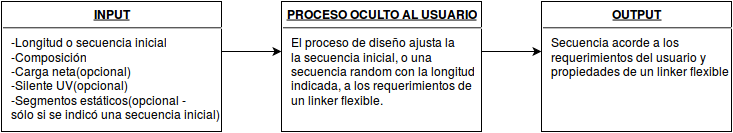
\includegraphics[width=\textwidth]{img/diagram.png}
 \caption{Esquema general de la herramienta implementada}
 \label{diagram}
\end{figure}


% \chapter{Introducci'on}
% 
% Existen dos tipos de citas bibliograf'icas: usa \verb|\citep{..}| para
% citas en \emph{par'entesis} y \verb|\citet{..}| para citas
% en el \emph{texto}. Por ejemplo, estudios reciente han mostrado nuevos e
% interesantes modelos que se pueden aplicar para reformular teor'ias
% f'isicas~\citep{NewCam97}. Mientras que, el trabajo de \citet{Rofl06} fue
% considerado muy divertido por una significativa fracci'on de la comunidad
% de investigadores. Tambi'en es posible citar a varios trabajos en una sola
% referencia \citep{Lamport86,Knuth84}.



\section{Estructura de este trabajo}

Este primer capítulo introductorio está dividido en dos secciones que presentan los aspectos necesarios para comprender el trabajo realizado, el cual se centra en el diseño de nuevas secuencias linkers con 
propiedades conformacionales definidas, restringiendo cualquier actividad biológica y elemento estructural no deseado.
En la primer sección (\ref{proteinLandscape}) se describe el amplio panorama conformacional y funcional que pueden presentar las proteinas.
% identificando cuáles son los elementos funcionales que pueden de acuerdo a las propiedades estructurales que adquieren.
% in-vivo, describiendo cuales son los posibles destinos de las proteinas desde que son sintetizadas en el ribosoma y a lo largo de su etapa funcional en la célula. 
% Se desarrollan los conocimientos actuales acerce del perfil de conformaciones y funciones conocidas, y las propiedades secuenciales asociadas con estas.
% Se intenta describir como estos conocimientos actuales sobre las propiedades conformacionales y funcionales de las proteinas se trasladan en el desarrollo 
% de un amplio abanico de metodos y herramientas bioinformaticas que, a su vez, permiten nuevos avances en los conocimientos subyacentes.
En la sección siguiente (\ref{proteinEngineering}) se desarrolla el tema de ingeniería de proteínas, intentando mostrar los conceptos más relevantes del área asociados a este trabajo, 
introduciendo el problema de cómo y por qué diseñar nuevas secuencias linker.

En el capítulo \ref{method} se describe el desarrollado para obtener secuencias linker, indicando los fundamentos y detalles de la implementación.
% , limitaciones y aspectos relevantes de su utilización.

En el capítulo \ref{tools} se detalla los distintos recursos utilizados para evaluar las propiedades de interés sobre la secuencia, describiendo el objetivo de cada evaluación y los fundamentos de cada método. 

En el capítulo \ref{manual} se documentan todos los aspectos necesarios para poder hacer uso de la herramienta.

En el capítulo \ref{results} se muestran, en primer lugar, las evaluaciones realizadas para obtener los parámetros óptimos de ejecución. 
Además, se evalúan distintas propiedades de la herramienta resultante y su ejecución analizando, luego, las secuencias obtenidas. 

Finalmente, el capítulo \ref{conclusiones} contiene las discusiones relevantes, conclusiones y trabajo a futuro.












\section{Perfil conformacional y funcional de proteinas}
% \label{proteinLandscape}


Las primeras proteínas estudiadas poseían una tendencia intrínseca a plegarse espontáneamente para dar una única estructura tridimensional.
Los estudios estructurales sobre estas proteinas indicaban que la información requerida para adoptar esta estructura única estaba codificada en su secuencia primaria y que, además, se correspondia con un mínimo global sobre el
perfil de energía libre asociado al polipéptido.  
% Much research has been carried out since then into the mechanism of folding, both under carefully controlled conditions in the laboratory and within cellular environments
La secuencia de aminoácidos determina una única estructura resultante, conocida como estructura nativa, la cual debería conferirle la función propia a la proteína.
% Comenzaron a surgir, entonces, distintos modelos para explicar cómo la estructura tridimensional confería las propiedades necesarias para  
Por un tiempo todo pareció indicar(y la mayoría creyó) que una estructura definida, aunque dinámica, era la base del mecanismo funcional.


% ACA PASO A LA IDEA DE POSIBLES DIFERENCIAS CON ESTE PARADIGMA CLASICO
El paradigma cambió rotundamente cuando se encontró que, a pesar de no poseer una estructura claramente determinada, una gran cantidad de péptidos y proteínas poseía funciones biológicas relevantes,
principalmente cumpliendo roles de señalizacion y regulación, siendo capaces de interactuar con diversos elementos a través de distintos mecanismos.
Los estudios posteriores afirmaron que, efectivamente, estos elementos pueblan un ensamble de conformaciones considerablemente distintas, que varían en el tiempo y también pueden variar entre 
las distintas regiones de una misma secuencia y con el contexto en el que se encuentran.
La definición de estado nativo, cuyo criterio es identificar la capacidad de realizar una función biológica, debe aplicarse también sobre esta diversidad de conformaciones.

El estudio de los perfiles de energía libre también se ve modificado e independientemente de su naturaleza estructural se encontró que el estado nativo representa, probablemente, sólo un mínimo local bajo condiciones fisiológicas.
Esto se debe a que distintos estados de agregación representan estados termodinámicamente muy estables correspondientes a minimos globales. 
A partir de esto surgen nuevas preguntas acerca de cómo se mantiene en la célula la solubilidad de los estados nativos.
La respuesta entra dentro de un concepto más amplio conocido como proteostasis(u homeostasis de las proteínas), que se desarrolla hacia el final de esta sección.

% Wright and Dyson 8 suggested that the existence of proteins with intrinsic protein disorder calls for a reassessment of the protein–structure– function paradigm.
Con el tiempo, entonces, se fue encontrando que las proteínas podían tomar caminos distintos al plegamiento espontáneo y llegan a poblar diversos estados bajo condiciones fisiológicas, 
entre los cuales se encuentra un amplio rango de conformaciones desordenadas y parcialmente plegadas, e incluso distintos estados de agregación con características estructurales diversas.
La idea central de esta sección es mostrar como las proteinas pueden, entonces, caer en un continuo de conformaciones estructurales y cómo las funciones 
emergen a partir de los distintos estados conformacionales y las transiciones dinámicas entre estos.
% from tightly folded single domains, to multidomain proteins that might have flexible or disordered regions, to compact but disordered MOLTEN GLOBULES and, finally, to highly extended, heterogeneous unstructured states.


% ESTO ES SOBRE MODULARIDAD, LO SAQUÉ DE LA SECCION, LO PUSE EN LA PARTE DE INGENIERÍA
% Los elementos estructurales y funcionales(y las relaciones entre estos) que permiten formar el paisaje resultante de conformaciones y actividades biológicas, 
% se muestran en la última sección como modulos individuales que proveen a la evolución la capacidad de crear nuevas proteínas compuestas, dando un punto de vista mas arquitectónico de éstas.
% que pueden componerse para dar origen a proteinas con funcionalidades compuestas.
% Algunos de estos módulos le brindan a la naturaleza la dinámica evolutiva necesaria para adaptar ciertas propiedades, mientras que otros permiten 
% proveen un completo set de elementos y mecanismos funcionales a la célula. 




































\subsection{Conformación de proteínas en solución} \label{conformationalLandscape}

El paradigma clásico de la biología estructural afirma que la secuencia primaria de una proteína contiene la codificación para que esta adopte una estructura definida única.
Si bien esta idea es una simplificación, dado que aún las proteínas mas estables son sistemas dinámicos con distintos grados de flexiblidad, este modelo se adapta a una gran cantidad de proteínas.
En éstas, el ensamble conformado por los estados accesibles en condiciones fisiológicas está limitado a un conjunto de estructuras que solo difieren en leves desviaciones del promedio del ensamble.
La dinámica de estas estructuras está dada por movimientos que van desde fluctuaciones rápidas de pequeña amplitud(del orden de \AA) hasta cambios relativamente lentos($\mu$s - $s$) que 
involucran modificaciones estructurales relevantes(plegamiento y movimientos asociados a la función).

Todos los movimientos son resultantes de rupturas y formaciones de interacciones provocadas por fuerzas de interacción las cuales, debido a su naturaleza débil, pueden romperse por efecto de la energía térmica, aún a temperatura ambiente.
Por lo tanto, a pesar de que estas proteínas puedan ser asociadas con estructuras estáticas definidas, las más mínimas fluctuaciones térmicas de la temperatura ambiente les permite explorar distintas conformaciones como parte de su actividad biológica.
En general, todos estos movimientos están asociados al mecanismos por el cual ejercen su función.
El conjunto de proteínas que posee estas características estructurales son las que denominamos plegadas y, debido a esta misma propiedad de poseer ensambles conformacionales con poca variabilidad, sus estructuras fueron las primeras que pudieron ser resueltas con precisión. 

No se puede pensar, sin embargo, que todas las proteínas tendrán esta conformación plegada.
Incluso entre las estructuras almacenadas en la PDB, no todas las proteínas muestran una conformación definida a lo largo de toda su secuencia, es así que muchas proteínas contienen segmentos no determinados de sus estructuras.
Usualmente esta falta de información es producto de regiones no definidas en el mapa de densidad electrónica que resulta del análisis de difracción por rayos X, 
correspondientes a ensambles de estructuras muy variables asociados a conformaciones flexibles o desordenadas. 
% Este tipo de segmentos es bastante común ya que sólo una pequeña porción de las estructuras en la PDB se encuentra totalmente libe de regiones con densidad electrónica no definida.
La simple pregunta sobre cuál es la conformación real que adoptan estos segmentos(donde se pierde la definición en la densidad electrónica), 
junto con la aparición de diversas proteínas funcionales sin una estructura plegada, 
llevaron a centrar la atención en 
segmentos/proteínas completas 
que no se adaptan correctamente al modelo clásico de plegamiento.
La búsqueda de respuestas a estos nuevos problemas llevo a descubir toda un area, quizás más compleja (e incluso más amplia), que la determinada por el paradigma clásico de proteínas plegadas.

% “why are some proteins highly sensitive in vitro to proteolysis?”, and “why do some proteins possess a particular behavior during the purification process?” 






% ******************************************
% IDPs SECTION
% ******************************************

Inicialmente, gran cantidad de evidencia soportaba la idea que la funcionalidad de las proteínas estaba asociada a su estructura tridimensional bien definida pero dinámica.
Consecuentemente, la idea de que muchas proteínas o regiones no adopten una estructura definida y posean una conformación intrínsecamente desordenada se creyó inaceptable. 
Por lo tanto, durante un largo tiempo fueron identificándose y estudiándose experimentalmente una a una, tratándolas como excepciones al modelo clásico.
Luego de este proceso, hace al menos una década, se formalizó la idea que el estado adoptado en condiciones nativas(funcionales) de muchas regiones o proteínas enteras podía ser intrínsecamente desordenado
(IDRs/IDPs = intrinsically disordered regions/proteins, a partir de ahora).
% Only around the turn of the millennium was it eventually formally raised in several conceptual papers [1–3], among them one in TiBS [4], that many proteins or regions of proteins 
% are intrinsically disordered (IDPs, or as originally termed, unstructured) under native, functional conditions. Although it was based on rather limited evidence, the groundwork of
% the new field was laid and sparked an immediate rapid expansion.
% Varios reviews en \cite{uversky2010understanding,dyson2005intrinsically}.
Es decir, existe un conjunto cada vez mas amplio de proteinas cuya secuencia no codifica un plegamiento determinado.
% Estamos hablando de un numero considerable de proteinas cuya secuencia encodes for the intrinsically unstructured proteins without specific structure.
Este reconocimiento trajo consigo una gran cantidad de preguntas que quedaron a la espera de aproximaciones/conocimientos de campo de la biofísica.
% These raise several compelling biophysical questions related to the structural characteristics of natively unfolded proteins.
¿Que tan desordenadas/desplegadas son estas proteínas?, ¿Son realmente conformaciones aleatorias o conservan una estructura residual?
¿Si poseen una estructura residual, cómo se clasifican sus conformaciones?
% How unfolded are these proteins? Are they random coils, or do they possess residual structure? If they have residual structure, how should they be classified?
% Based on the analysis of the available literature, it has been concluded that intrinsically unstructured proteins do not possess uniform structural properties, as expected for members of a single thermodynamic entity.
Un mayor avance requería la utilización de nuevas técnicas biofísicas\cite{eliezer2009biophysical}.

% Structural disorder can now be studied in great detail by several dozen experimental techniques 
% and the most spectacular advance has been achieved through the application of multidimensional NMR. This approach is often
% complemented by other structural techniques, such as small-angle X-ray scattering (SAXS), which is combined with advanced computational data integration based upon molecular dynamics (MD) simulations (Figure 1). These new
% approaches [22] enabled the characterization of the full structural ensemble of several dozen IDPs
% 

% CONCEPTOS GENERALES !!! REESCRIBIR-REORDENAR
En general, las IDRs/IDPs no poseen un núcleo hidrofóbico que les permita plegarse espontáneamente, lo que si ocurre en proteínas plegadas(en algo similar a un colapso hidrofóbico).  
En algunos casos, sin embargo, pueden formar estructuras desordenadas pero compactas, o algunos segmentos de la secuencia pueden adoptar transitivamente estructuras secundarias individuales.
% (which is equivalent to the ‘pre-molten globule’ proposed by Uversky 2 ). 
A pesar de esta tendencia desestructurada, debido a la naturaleza heteropolimérica de las proteínas, es probable que nunca adopten 
conformaciones totalmente aleatorias(donde las conformaciones solo estan restringidas por impedimentos estéricos), aún en entornos altamente desnaturalizantes donde normalmente se pierden las propiedades estructurales.
Es decir, incluso los estados mas desestructurados mantienen una cierta tendencia a formar elementos estructurados locales, caracterizados por estructuras secundarias transitivas o núcleos hidrofóbicos.
La existencia de estos residuos de estructura se han detectado en proteinas estructuradas sometidas a altas concentraciones de desnaturalizantes fuertes. 
% Thus, coil-like ID proteins are not completely random, but are characterized by the presence of some residual (and highly flexible) structure. 

Como vamos a ver, esta leve estructura residual(latente o transitiva) es muy importante y representa gran parte de las capacidades funcionales en IDRs/IDPs.
Por lo tanto, se puede decir que las IDRs/IDPs poseen propiedades conformacionales mucho mas complejos que polipéptidos con estructuras totalmente aleatorias y que esta excepcional heterogeneidad estructural
representa tambien un problema crítico a la hora de estudiarlas experimentalmente y caracterizarlas.
% The existence of preferred limited proteolysis cutting sites also indicates that the native conformation prevails

A partir de esta descripcion estructural se puede entender por qué el término inicial asignado a estas proteínas (proteínas desestructuradas) ha quedado obsoleto.
La única característica distintiva de las IDRs/IDPs es, entonces, su inhabilidad para plegarse en una estructura tridimensional única.
A pesar de esta falta de estructura única definida, como se vió, presentan una 
gran diversidad de propiedades estructurales y, lo que es mas importante, estas están relacionadas con las funciones de la proteína. 
Por lo tanto, el término general para describir estas proteínas es, simplemente, ``desordenadas''. 
Este término se aplica tanto a las regiones que forman parte de proteinas plegadas mas grandes, como a secuencias que carecen totalmente de estructura plegada. 
Como veremos, el mosaico estructural que ofrece la variedad de secuencias conformadas por regiones con propiedades estructurales diversas es fundamental para obtener el extenso catálogo de funcionalidades existentes.    




% ******************************
% PROPIEDADES ESTRUCTURALES
% ******************************

Ahora que sabemos que las IDRs/IDPs no están completamente libres de restricciones estructurales, nos concentraremos en describir cuales son las características de su conformación:
Las IDRs/IDPs consisten en estructuras altamente dinámicas que se interconvierten en diferentes escalas de tiempo.
Estas estructuras varían desde estados completamente sin estructura(polipéptidos nativos sin plegamiento) hasta estados parcialmente plegados(sin estructuras secundarias definidas), o incluso ensambles desordenados pero con ciertas
estructuras secundarias claramente determinadas.
La distribución de estas estructuras está cambiando continuamente en el tiempo. 
Es decir, la estructura tridimensional que podemos ver en un instante dado será diferente de la que veremos en otro momento.

A pesar de esta dinámica estructural, sin embargo, las IDRs/IDPs carecen de cualquier tipo de estructura secundiaria(o terciaria) estable bajo condiciones fisiológicas.
Las estructuras residuales que describimos como parte del ensamble, a pesar de ser transitorias, tienen un papel relevante en el cumplimiento de la función asociada a la proteína.
Cualquier IDR/IDP contiene una gran cantidad de este tipo de elementos estructurales, algunos con gran potencial para plegarse, otros con capacidades de plegamiento diferencial(en algún contexto determinado) 
y otros sin posibilidad alguna de adquirir una estructura determinada.
De esta última descripción se puede imaginar que, probablemente, ninguún IDR/IDP adoptará una conformación totalmente desordenada a lo largo del tiempo(aunque tampoco estará completamente plegada), por el contrario, se tendrá una gran variedad
de posibles mosaicos con distintas proporciones y tipos de elementos estructurales.

Este perfil conformacional, junto con las proteinas plegadas que describimos al principio de esta sección, forma un continuo estructural que puede verse en la figura \ref{conformationContinuum}.
El extremo izquierdo representa el perfil de las proteinas completamente plegadas. 
En \cite{gall2007intrinsic} se ve que, incluso en la PDB donde las estructuras almacenadas están sesgadas hacia el perfil de proteínas plegadas(porque son las más simples para cristalizar), las conformaciones totalmente ordenadas son 
poco abundantes y que la mayoría de las estructuras posee al menos un segmento desordenado.
Este y otros estudios parecen indicar que el comportamiento de las proteinas totalmente plegadas es la excepción más que la regla, y que la mayoria de las secuencias tienen regiones desordenadas.


\begin{figure}[htbp]
\centering
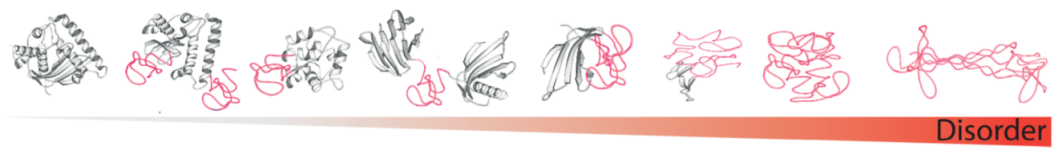
\includegraphics[width=1.0\textwidth]{img/conformationContinuum.png} 
\caption{ Continuo estructural: Los segmentos desordenados pueden comprender solo un pequeño conjunto de aminoácidos dentro de las proteínas u ocupar grandes segmentos de ésta, resultando en un
perfil similar al que se ve en la figura. De izq. a derecha: estructura totalmente ordenada; extremos N y C terminales desordenados; región linker desordenada uniendo dominios globulares; loop desordenado;
dominio completamente desordenado; proteína desordenada con elementos estructurales residuales; proteína desordenada sin elementos estructurales definidos pero con conformación colapsada; proteína totalmente desordenada.
}
\label{conformationContinuum}
\end{figure}


% CLASIFICACION
A pesar que en algunos estudios se intentan clasificaciones estructurales de las IDRs/IDPs, preferimos mantener acá la idea de un continuo conformacional.
Más adelante, cuando hablemos de las funcionalidades podremos esbozar algunas clasificaciones y nombres para los estados generalmente poblados por estas proteínas. 
% However, already in some early studies, it was indicated that IDPs/IDRs could be crudely grouped into two major structural classes, proteins with compact and extended disorder, 
% indicating that functional IDPs can be less or more compact and possess smaller or larger amount of flexible secondary/tertiary structure.

% Para dejar las cosas un poco mas claras vamos a intentar realizar una clasificacion de las ID proteins en terminos estructurales.
% Usando esta analogia(similitud) con los estados intermedios del plegamiento, en \cite{uversky2010understanding} it has been established that ID proteins and regions under physiological conditions in vitro might 
% contain collapsed-disorder (i.e., where ID is present in a form of molten globules) and extended-disorder (i.e., regions where ID is present in a form of random coil or pre-molten globule)

% \begin{itemize}
%  \item Collapsed disorder:  The structural properties of the molten globule (which was originally described as universal folding intermediate of globular proteins) are well known and
% have been systematized in number of reviews. The protein molecule in this intermediate state has no (or has only a trace of) rigid cooperatively melted tertiary structure. 
% However, it is characterized not only by the well-developed secondary structure, but also by the presence of some topology, i.e., relatively fixed mutual positioning of the secondary structure elements.
% A considerable increase in the accessibility of a protein molecule to proteases was noted as a specific property of the molten globule.
% The transformation into this intermediate state is accompanied by a considerable increase in the affinity of a protein molecule to the hydrophobic fluorescence probes
% 
%  \item Extended disorder: A significant number of sequences encodes for the extendedly disordered proteins that are characterized by low sequence complexity. Are these proteins
% random coils, or do they possess residual or transient structure? If they have residual or transient structure, how should they be classified? Based on the analysis of the available literature, it has been concluded that such proteins do not possess uniform structural properties, as expected for members of a single thermodynamic entity.
% In fact, they may be divided into two structurally different groups, intrinsic coils and intrinsic pre-molten globules, tal como se realiza en \cite{uversky2002natively}: 
%  Proteins from the first group have hydrodynamic dimensions typical of considerably unfolded polypeptide chain in poor solvent (see below and fig. 1), and do not possess any (or almost any) ordered secondary structure. 
% Proteins from the second group are more compact (see below and fig. 1), and exhibit some amount of residual secondary structure. However, they are still less dense than native globular or molten globule proteins
% \end{itemize}

















% DIFERENCIAS EN EL PERFIL DE ENERGIA LIBRE
Todo lo descrito previamente acerca de proteínas plegadas, sus diferencias con el perfil de las IDRs/IDPs, y la estabilidad de los distintas conformaciones del ensamble, 
puede entenderse mejor si se analizan las superficies de energía libre asociadas. 
En la figura \ref{idp-folded-EnergyLandscape} se ven ejemplos de estos paisajes energéticos para tres ejemplos representativos de todo el continuo de conformaciones vistas.

El gráfico que se ve en la figura \ref{idp-folded-EnergyLandscape}\textbf{(a)} muestra el perfil de energía libre frente a los cambios conformacionales asociados para una proteína plegada.
El perfil con la forma similar a un embudo, característico de este tipo de proteínas, representa lo que se describió previamente sobre éstas, a través del plegamiento alcanzan una estructura ``única'' que 
representa el mínimo global de energía. 
Como detallamos, esta estructura única representa en realidad un ensamble de conformaciones con muy pocas variaciones, capaz de ser representado por una estructura promedio.
Diversos estudios sobre el proceso de plegamiento resultaron en una gran diversidad de teorías sobre los detalles de este paisaje energético y como se relaciona con el proceso de plegamiento.
Sin embargo, lo mas relevante se obtiene de observar la forma en que se ubican los mínimos de energía y la amplitud de éstos, lo que nos dará una idea del ensamble real que encontraremos en condiciones fisiológicas.
% Folded proteins have a "funnel-shaped" global free energy minimum, where the lowest energy state corresponds to the 11native structure, and the width of the unique global energy minimum
% determines the conformational entropy of the native state.

A medida que nos movemos hacia la derecha en el continuo de conformaciones posibles de la figura \ref{conformationContinuum}, los segmentos desordenados 
modifican el perfil energético aplanando la superficie en el mínimo global de energía. 
Este cambio(graficado en la figura \ref{idp-folded-EnergyLandscape}\textbf{(c)}) representa la existencia de nuevas estructuras con una diferencia conformacional considerable con respecto al resto de las estructuras del ensamble, 
pero que están separadas entre si por barreras energéticas pequeñas. 

El perfil energético continua aplanándose a medida que aumentan las regiones desordenadas de la proteína. En la figura \ref{idp-folded-EnergyLandscape}\textbf{(b)} se ve el perfil 
correspondiente a una proteína con una conformación completamente desordenada. 
Como se puede ver, el paisaje entero queda descrito por una superficie semiplana con múltiples conformaciones asociadas al mínimo de energía, 
asociadas a valores de energía aproximadamente iguales y separados por barreras energéticas muy pequeñas.
Estas barreras representan las transiciones rápidas y frecuentes entre las distintas conformaciones y que resultan en las propiedades observadas experimentalmente
en solución: un conjunto heterogéneo de conformaciones fácilmente maleable por cambios en el medio. 

\begin{figure}[h]
\centering
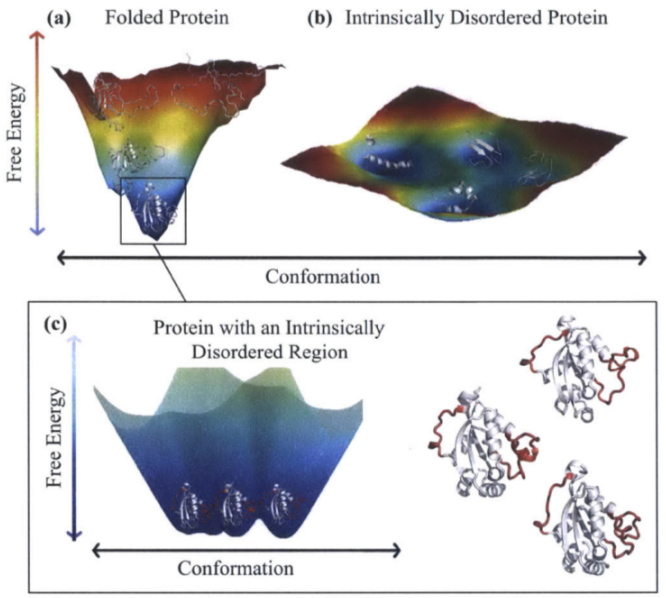
\includegraphics[width=0.7\textwidth]{img/idp-folded-EnLandscape.png} 
\caption{Diferencias en el paisaje energético entre polipéptidos que adquiren estructuras plegadas, IDRs e IDPs }
\label{idp-folded-EnergyLandscape}
\end{figure}


En base a esto, se ve que una descripción detallada de IDRs/IDPs requeriría conocer el ensamble de estados posibles junto con las velocidades de interconversión entre estos.
% Thus, a comprehensive characterization of an IDP consists of an ensemble of states and the transition rates between them.
% Además, este perfil energético se ve modificado por distintas condiciones como modificaciones post-traduccionales, condiciones del medio, presencia de ligandos,etc.
% Las poblaciones encontradas en los distintos estados cambian con las diferencias en estas condiciones
% As a result, the populations of individual conformations within the ensemble change , también, under different conditions. 
% Para estudiar experimentalmente estas proteínas, entonces, es normal utilizar técnicas experimentales que no se basan en el promedio de conformaciones.
% and is best measured by experimental techniques that prevent conformational averaging.
Todas estas propiedades y las velocidades de las transiciones en el ensamble son difíciles de capturar experimentalmente(y computacionalmente también), aún usando técnicas experimentales que no se basan en promedios de conformaciones.
Los estudios sobre este tipo de proteínas, entonces, se han enfocado en analizar los estados termodinámicamente accesibles como entidades discretas.
% En lugar del análisis estructural clásico basado en dominios globulares, que usamos para podemos describir estos conjuntos conformacionales en términos de los promedios y desviaciones estándar
% de la distancia entre los extremos de la secuencia, el radio hidrodinámico, el contenido en estructura secundaria y otros parámetros (20).
Como veremos a continuación y en las próximas secciones, esta idea, si bien sabemos que es una descripción incompleta, permite modelar de forma discreta los elementos funcionales relevantes, sirviendo como base para estudios posteriores.
Este modelo puede extenderse si se representan también las probabilidades de ocurrencia para distintas conformaciones individuales en el ensamble, obteniendo asi un modelo mas dinámico del sistema.
% Thus, the dynamic nature of IDPs is best modeled by statistical approaches that describe the probabilities of individual conformations in the ensemble, 






% ***************
%  INDUCED FIT:
% ****************
% Además, este perfil energético se ve modificado por distintas condiciones como modificaciones post-traduccionales, condiciones del medio, presencia de ligandos,etc.
Los ensambles conformacionales, además, pueden verse modificados por distintas situaciones como cambios en las condiciones del entorno, modificaciones post-traduccionales, presencia de ligandos, etc.,
lo que modifica no sólo los estados accesibles, sino también la distribución de poblaciones que se encuentran en cada uno.
Una propiedad particular dependiente del contexto, encontrada en los ensambles conformacionales asociados a IDRs/IDPs, es la capacidad de adquirir nuevos elementos estructurales ordenados estables luego de la unión a ciertos ligandos
(proceso conocido como textit{binding \& folding}\cite{dyson2005intrinsically}). 
Esta propiedad se hace mas relevante de investigar cuando se sabe que, generalmente, está asociada a su funcionalidad biológica y ocurre previamente o durante la realización de esta función.
% Although disordered proteins exist as dynamic structural ensembles without fixed(estable!!!) tertiary structures, there is evidence that many flexible regions of proteins undergo coupled binding and folding \cite{dyson2005intrinsically}. 
% A large decrease in conformation entropy accompanies such disorder-to-order transitions. 

Una gran cantidad de IDRs/IDPs, entonces, se ven estabilizadas termodinámicamente mediante la unión a ligandos específicos(generalmente otras proteínas, DNA, membranas, etc)
% In other words, intrinsically unfolded proteins in vivo are likely to be stabilized by functional binding to specific targets and ligands 
% (such as a variety of small molecules, substrates, cofactors, other proteins, nucleic acids, membranes and so on). 
% Many intrinsically disordered proteins undergo transitions to more ordered states or fold into stable secondary or tertiary structures on binding to their targets — that is, they undergo coupled folding and binding processes.
Los complejos funcionales entre IDPs y sus ligandos son formados por interacciones intermoleculares específicas y modifican el paisaje energético visto previamente, generando nuevos estados definidos de mínima energía.
Esta diferencia se ve en \ref{idpBindingEnLandscape}.
% Functional complexes of IDPs with their partners are formed via the specific intermolecular interactions that change the energy landscape creating more defined free energy minima.


\begin{figure}[h]
\centering
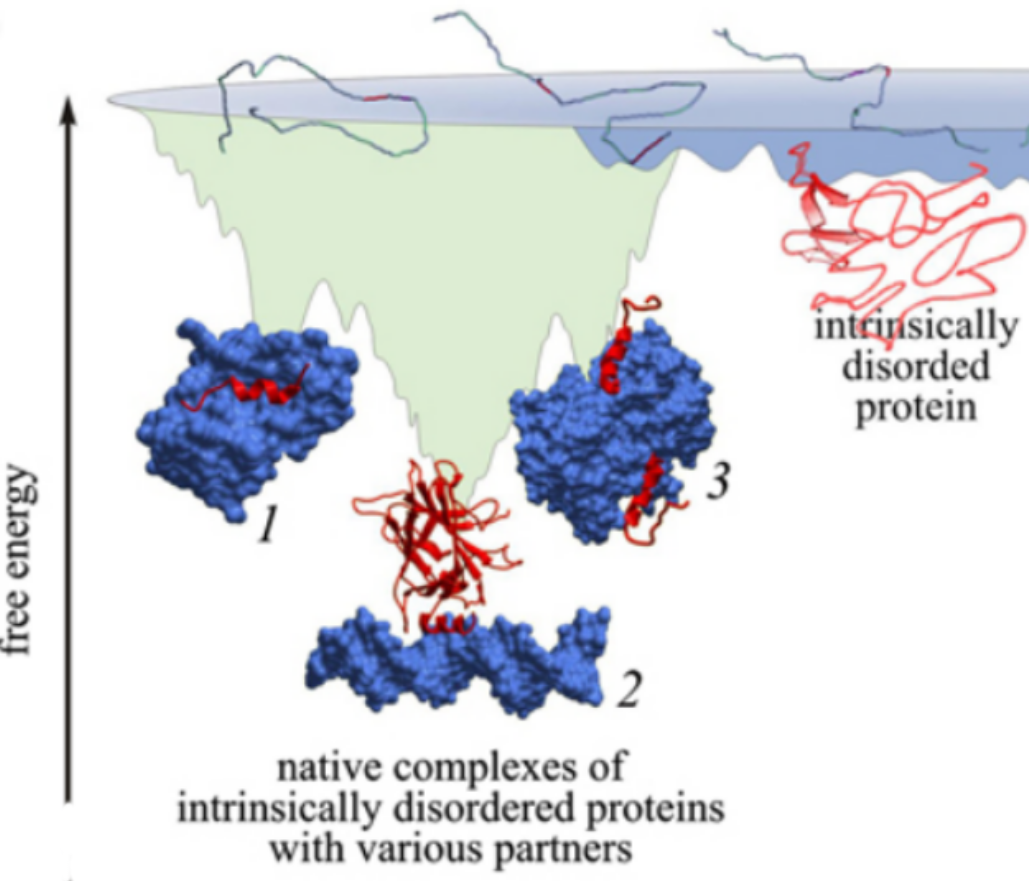
\includegraphics[width=0.7\textwidth]{img/idp-binding-EnLandscape2.png} 
\caption{Perfil energético de los estados de IDRs/IDPs. Los segmentos desordenados pueden plegarse para dar estructuras ordenadas estables a través de interacciones con ligandos específicos.
Esta situación se da cuando la formación del complejo resulta en una disminución de energía libre. 
% Disordered segments of these proteins can gain ordered structure at the interaction with specific binding partners in a case if the free energy of such complexes is lower 
% than the free energies of the intrinsically disordered protein and its partner. 
Por si sólo, el polipéptido presenta un paisaje energético semiplano(sección derecha). La interacción con distintos ligandos(1,2,3) resulta en nuevos estados termodinámicamente estables.
Figura extraída de \cite{turoverov2010protein}}
\label{idpBindingEnLandscape}
\end{figure}

Las IDRs/IDPs pueden adoptar esta conformación plegada si la energia del complejo formado es menor que la energía libre correspondiente al segmento desordenado y su ligando, previo a la interacción.
% IDPs fold as a whole while interacting with their partners, if the free energy of complex is lower than the free energies of IDP and its partner before their interaction.
En general, sólo un segmento desordenado con características anfipáticas es el que está involucrado en el proceso de unión y plegamiento, en este caso el segmento se denomina elemento de reconocimiento(RE=recognition element). 
% More often, however, only a part of an IDP, a specific recognition element, which is a relatively short amphipathic linear motif contained within long disordered sequence, is involved in the coupled folding and binding events
% Induced fit interactions can also occur between structural domains and relatively large natively unstructured regions of other proteins. 
% The natively unstructured region is then induced to form a stable structure, but only in the presence of the interacting structural domain.
Este tipo de transiciones ante la unión a ciertos ligandos, involucrando regiones cortas de la secuencia, provee una combinación de alta especificidad y baja afinidad que hace a este tipo de elementos extremadamente útiles en procesos de señalizacion y regulación.
% This disorder-to-order transitions, in turn, leads to a combination of high specificity and weak affinity, a pair of linked features that are extremely useful for signalling and regulation.

Una pregunta que aparece naturalmente al intentar estudiar este proceso es si el elemento estructural ordenado es generado durante la unión al ligando 
o si pertenece al conjunto de elementos estructurales encontrados transitivamente en las IDRs/IDPs y, al unirse, se hace parte de la conformación estable.
% An often-raised issue with respect to IDP binding is whether folding occurs before or after binding (termed conformational selection and induced folding, respectively).
% Detailed studies suggest that folding can occur both before and after binding in distinct cases
Estas dos opciones se reflejan en los modelos de selección de conformación y el de unión y plegamiento simultáneo.
% There are two major models describing the coupled folding and binding process in proteins, the conformational selection model and the simultaneous binding and folding model, also known as the induced folding model.
% The conformational selection mechanism is based on the hypothesis that when free in solution, IDP populates the ensemble of conformations and, from this ensemble, the binding partner “chooses” or
% “selects” a specific conformation which closely approximates that of the bound form. An illustrative example of the conformational selection mechanism in the recognition process is
% so-called “preformed structural elements” or elements of local residual structure, which are frequently observed in IDPs and which are crucial for the IDP interactions with its specific
% partners
% 
% Induced folding model postulates that IDP associates with its binding partner in a fully disordered state and subsequently folds in association with the target protein. 
% In molecular recognition, this model is exemplified by so-called molecular recognition elements or features, which are short (around 20 residues) structural elements which are found 
% within the regions of disorder and which mediates certain classes of binding events of disordered regions undergoing a disorder-to-order transition into a specific structure that is stabilized by binding to its partner.
% These recognition motifs can fold into $\alpha$-helix, $\beta$-strand, or form irregular structure on binding to a target protein
Obviamente, en realidad, puede ocurrir cualquiera de estos dos mecanismos o una combinación de los dos.
% Obviously, in reality, either one of the outlined above mechanisms, the conformational selection model or the induced folding model, or some combination of the two can be used.
Esto se ve representado en la figura \ref{idpBinding}



\begin{figure}[h]
\centering
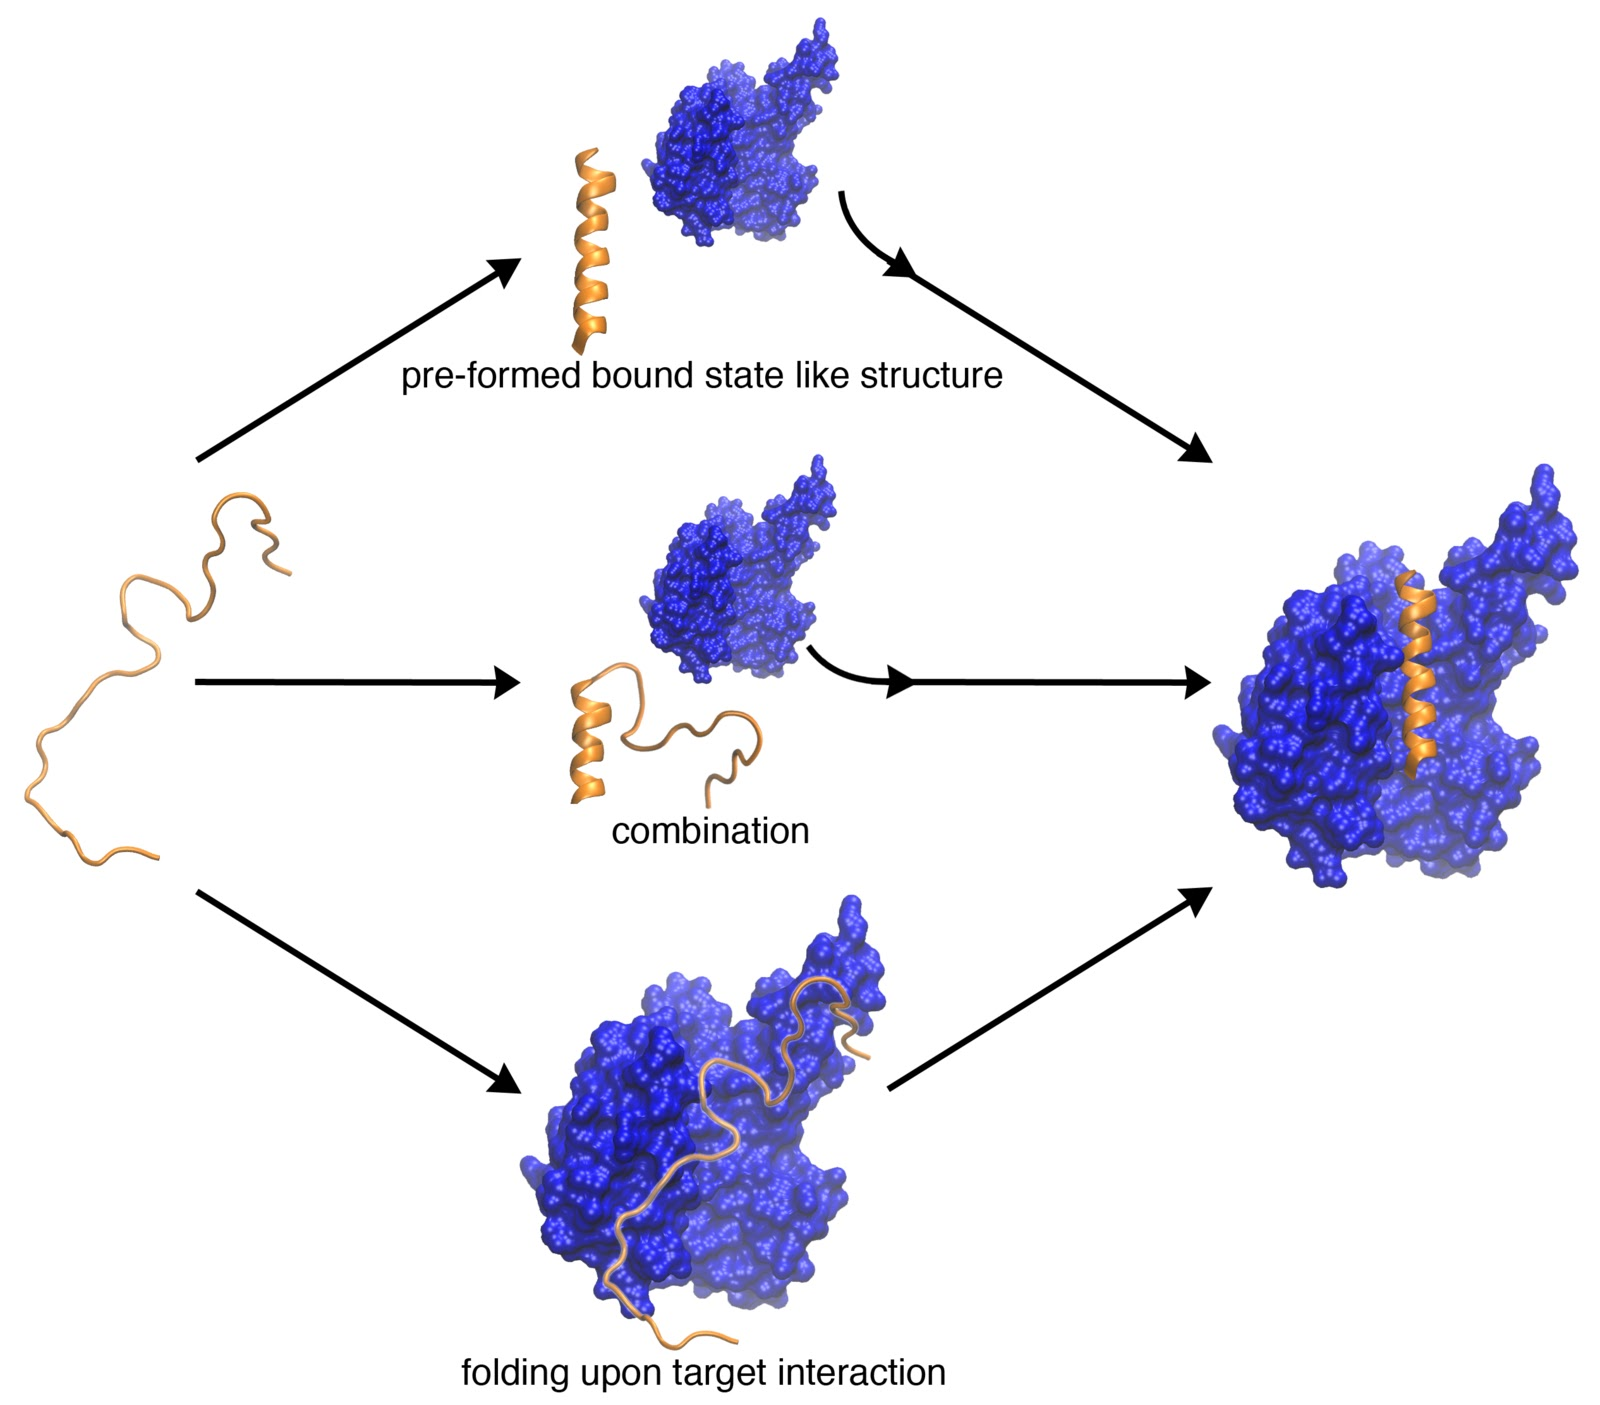
\includegraphics[width=0.8\textwidth]{img/PSE-MoRE.jpg} 
\caption{Distintos modelos de \textit{binding \& folding}} 
\label{idpBinding}
\end{figure}



% ESTO TIENE QUE IR DESPUES DE TODO EL DESARROLLO DE INDUCED FIT
% En base a estas propiedades estructurales y el induced fit, en el review \cite{dunker2001intrinsically} se plantea una clasificacion del desorden en dos categorias: intermittent and constant.
% The former describes protein molecular recognition domains and other regions that undergo order/disorder transitions to carry out binding or other functions. The latter describes regions such as
% proteinaceous detergents, flexible linkers, entropic springs, entropic clocks and entropic bristles that remain disordered while carrying out function.

A partir del estudio sobre este proceso de 'binding \& folding', basándose en los modelos previos, se encontraron algunos conceptos importantes inesperados.
% Two unexpected and important concepts have also emerged in the binding-folding paradigm.
En primer lugar se encontró que dos IDRs/IDPs pueden unirse en un proceso de unión y plegado mutuo \cite{bhattacherjee2012coupled},
es decir, una IDR/IDP también puede funcionar como ligando y plegarse en este proceso. 
% One is the intriguing observation that two IDPs/IDRs can bind each other in a process of mutual (synergistic) folding [47].
Por otro lado, se encontró que el proceso de unión y reconocimiento del ligando puede proceder aún sin necesidad de plegamiento. 
% The other, even more confounding finding, is that recognition can proceed even in the lack of folding in the bound state. 
Esto tiene implicancias importantes en los aspectos funcionales ya que, como se había predicho, la capacidad de unión a ligandos dependía de la formación de este elemento estructural.
Gran cantidad de ejemplos de este tipo de uniones(determinados complejos ``fuzzy'') extienden la idea de desorden no sólo a proteínas en solución, sino también a interacciones formando complejos. 
% The many examples of such ‘fuzzy’ interactions demand the extension of the concept of structural disorder to the bound state.













% COMPOSICION CARACTERISTICA DE IDPs
% Desde que se identificaron las IDRs/IDPs como entidades de interés biológico, 
Además de todas las propiedades conformacionales que se analizaron sobre IDRs/IDPs,
% , tanto sobre las proteínas plegadas como sobre la extensa continuación del mosaico formada por IDRs/IDPs,  
muchos estudios se hicieron para intentar identificar cómo están codificadas estas propiedades en la secuencia de la proteína.
Como se describió previamente, la secuencia primaria de una proteina plegada codifica el proceso de plegamiento y la estructura única final. 
Al identificar a las IDRs/IDPs cómo entidades estructuralmente diferenciables se podría pensar que la estructura primaria de éstas determina, también, su falta de estructura tridimensional definida.
% Identification of IDPs as unique entities belonging to a new protein tribe is directly related to the recognition that their amino acid sequences are dramatically different from those of ordered proteins.
Esto tiene como corolario la idea que las secuencias de ambos conjuntos (proteinas ordenadas y proteínas desestructuradas) deberían ser diferenciables entre si.
% since amino acid sequence determines three-dimensional structure, amino acid sequence should also determine lack of three-dimensional structure.

La ausencia de una estructura definida en IDRs/IDPs es atribuida a las características particulares de sus secuencias de aminoácidos las cuales pueden resumirse en la presencia de númerosos 
grupos cargados no compensados(generalmente con carga negativa) y un bajo contenido de residuos hidrofóbicos.
% the absence of regular structure in these proteins has been explained by the specific features of their amino acid sequences including the presence of numerous uncompensated charged groups (often negative); 
%  i.e., a high net charge at neutral pH, arising from the extreme pI values in such proteins , and a low content of hydrophobic amino acid residues.
% Several ID proteins have been discovered due their unusual amino acid sequence compositions
La relación entre esta combinación de baja hidrofobicidad y alta carga neta y la falta de una estructura definida puede explicarse desde el punto de vista físico:
los altos valores de carga neta producen efectos de repulsión entre las cargas de los residuos, mientras que la baja hidrofobicidad previene la compactación de la estructura lineal
(las interacciones hidrofóbicas son una de las principales fuerzas que interviene en el proceso de plegamiento).
El resultado es una estructura con tendencia a mantener una conformación desplegada, característica de las IDRs/IDPs.

% It has been concluded that the combination of low mean hydrophobicity and relatively high net charge represents an important prerequisite for the absence of compact structure in proteins under physiological conditions.
% This observation was used to develop a charge-hydropathy (CH) plot method of analysis that distinguishes ordered and disordered proteins based only on their net charges and hydropathies.
% From the physical viewpoint, such a combination of low hydrophobicity with high net charge as a prerequisite for intrinsic unfoldedness makes perfect sense: high net charge leads to charge-
% charge repulsion, and low hydrophobicity means less driving force for protein compaction. In other words, these features are characteristic for ID proteins with the coil-like (or close to coil-
% like) structures.

% 
% 
% ****SI HACE FALTA PUEDO AGREGAR ESTE PARRAFO SOBRE ALGUNAS CARACTERISTICAS EXTRA DE LAS SECUENCIAS, O REFERENCIAR ALGO, 
% 
% The disordered proteins are significantly depleted in bulky hydrophobic (Ile, Leu, and Val) and aromatic amino acid residues (Trp, Tyr, and Phe), which would normally form the hydrophobic core of a folded globular protein, 
% and also possess low content of Cys and Asn residues.
% The depletion of ID protein in Cys is also crucial as this amino acid residue is known to have a significant contribution to the protein conformation stability via 
% the disulfide bond formation or being involved in coordination of different prosthetic groups.
% On the other hand, ID proteins were shown to be substantially enriched in polar, disorder-promoting, 
% amino acids: Ala, Arg, Gly, Gln, Ser, Glu, and Lys and also in the hydrophobic, but structure braking Pro.


% The fact that natively unfolded proteins, with their depleted hydrophobicity, are noncompact under physiological conditions indicates that ‘salted water’ (typical ‘physiological’ buffer contains 100–150 mM NaCl) does not represent for them a poor solvent.
% In other words, these conditions do not force polymer segments to interact specifically with each other and, thus, do not force them to be effectively excluded from the solvent.
% On the other hand, it has already been noted that even high concentrations of strong denaturants do not represent a good solvent for a polypeptide chain encoding for a typical globular protein, and a globular protein was assumed to never be a random coil.


% Por lo tanto, a signature of probable intrinsic disorder is the presence of low sequence complexity and amino-acid compositional bias, with a low content of bulky hydrophobic aminoacids (Val, Leu, Ile, Met, Phe, Trp and Tyr), which would
% normally form the core of a folded globular protein, and a high proportion of particular polar and charged amino.....
% ESTAS PROPIEDADES SE HAN UTILIZADO PARA LAS PRIMERAS GENERACIONES DE HERRAMIENTAS PARA PREDECIR DESORDEN A PARTIR DE LA SECUENCIA.
% Luego se crearon predictores que analizaban la secuencia usando ventanas(PONDR)

% In addition to amino-acid composition, the disordered segments have also been compared with the ordered ones by various attributes such as hydropathy, net charge, flexibility index, helix
% propensities, strand propensities, and compositions for groups of amino acids such as W + Y + F (aromaticity).

% Estas propiedades fisicoquimicas tambien fueron incluidas para los predictores.






% COMENTARIOS APARTE SOBRE LA REGULACION DE IDPs EN LA CELULA
En términos biológicos las diferencias secuenciales entre las IDRs/IDPs y los segmentos o proteínas totalmente plegadas, además de las diferencias conformacionales antes vistas(y de las diferencias funcionales que veremos), 
indican que se tratan de entidades separadas dentro del complejo perfil del proteínas naturales existentes.
% The fact that the sequences of ordered and disordered proteins and regions are noticeably different suggested that IDPs clearly constitute a separate entity inside the protein kingdom, 
% that these proteins can be reliably predicted using various computational tools,  and structurally, that IDPs should be very different from ordered globular proteins since peculiarities of amino acid sequence determine protein structure.
Esta claro, además, que no sólo son un elemento real y distinguible, sino que son abundantes en el proteoma, tienen propiedades muy diversas y cumplen funciones vitales para cualquier sistema biológico.
% It is clear now that the IDPs and IDPRs are real, abundant, diversified, and vital. The highly dynamic nature of IDPs and IDPRs is a visual illustration of the chaos.
% the evolutionary persistence of these highly dynamic proteins (see below), their unique functionality, and involvement in all the major cellular processes evidence that this chaos is tightly controlled
Todas estas propiedades hacen que parezca razonable que este tipo de proteínas este altamente regulada dentro de la célula \cite{gsponer2008tight,habchi2014introducing}.

% existen mecanismos para regular su degradacion(ver \cite{habchi2014introducing} Survival of IDPs in the Cell )
% Ademas por la extrema sensibilidad que tienen a la proteolisis in-vitro (lo cual es de esperar dada la confomracion extendida que adoptan), 





















































\subsection{Misfolding \& Agregación}



% INTRODUCCION
En el comienzo de la sección anterior describimos como algunas proteínas poseen conformaciones nativas con estructuras bien definidas,
esta restricción hace que, para poder funcionar correctamente, deban atravesar un proceso de plegamiento el cual ocurre, en condiciones normales, de manera muy rápida. 
Esto es posible ya que sus secuencias han evolucionado de forma tal que son capaces de alcanzar la estructura nativa(funcional) muy eficientemente, incluso en el complejo entorno celular.
% the sequences of these proteins have evolved in such a way that their unique native states can be found very efficiently even in the complex environment inside a living cell.
Sin embargo, a medida que el tamaño de la proteína aumenta, tambien aumenta la complejidad del proceso de plegamiento y este se vuelve propenso a errores,
lo que puede llevar a estas proteínas a adoptar conformaciones incorrectas(\textit{misfolded}). 
Los errores durante este proceso en el que se buscan las interacciones ``correctas'' entre los residuos pueden estar asociados a distintos factores(principalmente mutaciones), 
no sólo al tamaño de la proteína, ya que de por si el proceso de plegamiento es complejo. 
Por otro lado, si estos estados estructurales incorrectos mantienen su solubilidad pueden comenzar a acumularse en el entorno celular.

% as the size and complexity of proteins increase, therefore, the folding process becomes more complex,
% thus, errors along folding may occur and drive proteins to incorrectly folded or misfolded states, which may still possess certain stability in the physiological
% environment and, therefore, start to accumulate. 

Ademas de estos estados \textit{misfolded}, algunos intermediarios en el proceso de plegamiento pueden tener tiempos de vida considerables, poblando estados alternativos al plegamiento final.
% Intermediates with only partially formed structures can be populated and have significant lifetimes. 
Más alla de esto, una vez alcanzada la estructura final, diversas condiciones del entorno pueden producir que este se pierda y se adopte un estado no-plegado(\textit{unfolded}).
Por definición, cualquier proteína plegada que no esté en su estado nativo está en un estado \textit{misfoled}
% Protein misfolding is a wide-spread phenomenon. Any protein with changes in native structure which affect its normal function is misfolded. 
Las proteinas plegadas, entonces, no siempre se encuentran en su estado nativo dentro del entorno celular y pueden ocurrir acumulaciones de estados \textit{misfolded}.

% Under some conditions, then, proteins fail to fold properly or to remain correctly folded; this misfolding can lead to malfunction of proteins and the development of different pathological(cambio esta palabra??) conditions.
% In addition, events that may be termed 'misfolding' may take place during the search for the stable native-like contacts between residues. 
% That such complexities are seen even in the benign environment of a dilute solution of a pure protein suggests that they are even more likely to occur in the crowded environment of the cell.
Además del efecto que tiene adoptar un estado \textit{misfolded} sobre la función de la proteína, estos estados pueden también llevar a la formación de agregados entre proteínas
lo cual tiene, generalmente, un efecto muy grande en la célula/organismo.
Los estados \textit{misfolded} y agregados no son equivalentes ni dependientes entre si y 
% teniendo en cuenta el amplio rango de proteínas que no adoptan una única estructura nativa, 
la agregación de proteínas puede originarse a partir de distintos estados iniciales. 
% The terms 'misfolded' and 'aggregated' are not equivalent. 
Como se verá, la habilidad de una proteína a formar agregados desestructurados o estructuras amiloides depende de muchos factores, entre los cuales están claramente la secuencia y el entorno en que se encuentra.
De otra forma, las proteinas que adquieran conformaciones no estructuradas o que se encuentren en estados de plegamiento intermedios semi-estables tendrían una tendencia mucho mayor a la agregación y, sin embargo, esto no es así. 
% De hecho, sólo una pequeña fraccion de tales conformaciones tiene tendencia a formar agregados.

% But the idea that proteins can misfold, or fold to intermediates that may undergo undesirable reactions such as aggregation, provides insight into potential problems that can arise during folding even in the best designed environments.
% Folding and unfolding are also now known to be coupled to many of the key events in the functioning of a biological system, including translocation of proteins across membranes, protein trafficking, 
% secretion of extracellular proteins, and the control and regulation of the cell cycle.
% Thus, the failure of proteins to fold or to remain folded under physiological conditions is likely to cause malfunctions and hence disease







% **************** CONCEPTOS GENERALES DE AGGREGATION
La agregación se forma, entonces, por la asociación(interacción) anormal entre proteínas.
% The abnormal association of misfolded proteins usually leads to the formation of aggregates.
Si bien algunos agregados pequeños pueden mantener su solubilidad, en general los agregados precipitan en condiciones fisiológicas. 
% Small aggregates can remain soluble, but large protein aggregates precipitate out of solution under physiological conditions. 
A partir de las características morfológicas se pueden distingir escencialmente dos tipos de agregados: agregados amorfos y fibrillas amiloides.
% From the morphological point of view we can differentiate essentially two types of aggregates: amorphous aggregates and amyloid fibrils. 
Los primeros muestran una apariencia granular y consisten principalmente de proteínas en conformacione desplegadas, 
aunque presentan ciertas regiones con formacion de estructuras de hoja-$\beta$ generando la unión del agregado.
% Amorphous aggregates display a granular appearance when imaged by electron microscopy and consist mostly of disordered polypeptide chains, even if they
% display certain regions enriched in $\beta$-sheet structures, which glue the macromolecular assembly.
Por otro lado, las fibrillas amiloides poseen estructuras altamente ordenadas y repetitivas donde todos los polipéptidos que la componen adoptan un plegamiento en común.
% Amyloid fibrils are highly ordered and repetitive structures where all polypeptides adopt a common fold.
Si bien no se van a dar detalles puntuales de la estructura, se sabe que estas diferencias que se ven en la estructura macromolecular son el reflejo de diferencias en las interacciones y estructura a nivel atómico.
Estas diferencias estructurales también se reflejan a nivel biológico: los distintos tipos de agregados tienen afinidades diferentes frente al conjunto de chaperonas y, además, 
pueden acumularse en diferentes localizaciones celulares y ser degradados por mecanismos diferentes.
% These differences in structure also reflect biological differences; amyloid and amorphous beta-sheet aggregates have different chaperone affinities, accumulate in different cellular locations and are degraded by different mechanisms.
Por último, a diferencia de los agregados amorfos, las propiedades únicas de las fibrillasas 
amiloides han sido aprovechadas por distintos sistemas biológicos y pueden encontrarse versiones funcionales de éstas en distintos organismos\cite{fowler2007functional}.
% Contrary to amorphous aggregates, amyloid structures can fulfill biological functions, and functional amyloids are found in organisms from prokaryotes to humans \cite{fowler2007functional}.



% 
% Proteins might aggregate utilizing relatively short sequence stretches, usually organized in b-sheet-like assemblies. 

% La idea construida en las secciones previas, en la que un polipéptido nasciente podía adopar un continuo de conformaciones estructurales monoméricas y solo formar interacciones transitivas para cumplir si función, 
% debe extenderse ahora para incluir este conjunto de posibles estados de agregación. 
% En la sección previa se formó la idea que un polipéptido nasciente podía adoptar un continuo de formas conformacionales diferentes, con elementos diferentes


En la sección previa formamos la idea que un polipéptido puede adoptar un continuo conformacional de estructuras nativas las cuales, a su vez, pueden intercambiarse en el tiempo.
Desde el comienzo de esta sección se vió que el proceso para alcanzar estos estados nativos no es tan directo ni mucho menos simple, por lo tanto, se pueden llegar a caminos alternativos. 
Estos y otros conceptos están representadas en la figura \ref{aggregationDiagram}.

El camino central representa, en una dimensión, el continuo de conformaciones en solución que, como indican las flechas, puede ir en distintos sentidos y representa las posibles cambios dinámicos que pueden ocurrir desde la síntesis
de un polipéptido en el ribosoma y hasta ser degradado o perder esta conformación monomérica.
Los elementos de este camino pueden formar interacciones transientes con diversos ligandos(entre los cuales están otras proteínas) como parte de su función. 

% el continuo del proceso de plegamiento/no-plegamiento guiado principalmente partir de interacciones intramoleculares, que resulta en la amplia variedad de especies monoméricas existentes.


% conformaciones monoméricas 
% , resultantes del proceso  este proceo. 
% distintos procesos de plegamiento. 
% En esta sección    la idea de posibles agregaciones entre distintos estados conformacionales encontrados en la célula se plantea como caminos alternativos que pueden 

% Es decir, el camino 
% hemos creado la idea que los estados monomericos no son los unicos estados estables, que es posible que se originen estados agregados y que estos se generan principalmente a partir de proteinas que no se encuentran en una conformacion correctamente plegada.
% Sin emb
% Esta nueva idea se puede ver en 
% La idea construida en las secciones previas, en la que un polipéptido podía adopar un continuo de conformaciones estructurales monoméricas y formar interacciones transitivas con ligandos,

% En la figura pueden verse, de forma gráfica, distintos estados de agregacion como caminos alternativos al camino central de plegamiento/conformación monomérica.
% De la figura puede verse también, que los distintos procesos de agregación, que resultan en disintas estructuras agregadas, pueden originarse a partir de distintos estados iniciales de conformación.

\begin{figure}[h!,centered]
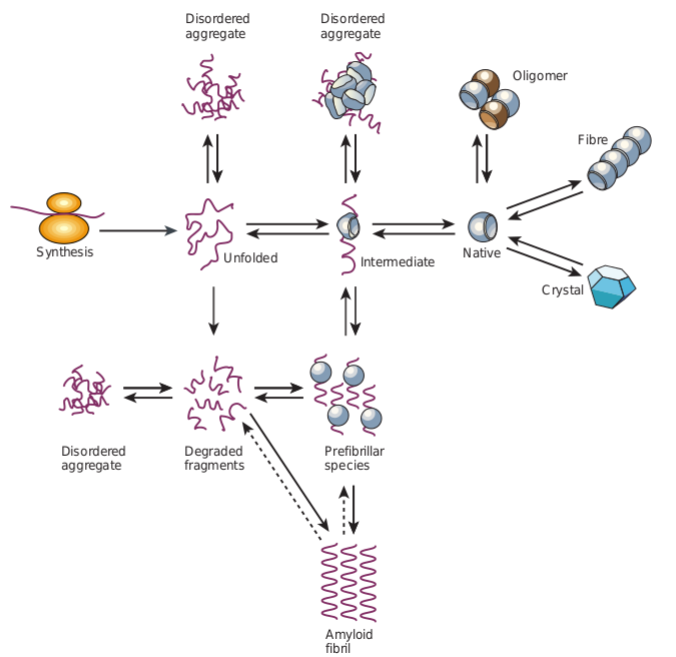
\includegraphics[width=\textwidth]{img/aggregationDiagram.png} 
\caption{Equilibrio de los estados de agregación} \label{aggregationDiagram}
\end{figure}


Al camino central de conformaciones monoméricas se le deben agregar todos los posibles caminos alternativos que involucran la formación de agregados que estamos describiendo en esta sección.
Se deben diferenciar los precipitados, en los que las proteínas mantienen la estructura nativa, y los agregados que, como mencionábamos antes, surgen a partir de nuevas estructuras no-nativas.
% One should distinguish between precipitates, in which proteins maintain the native folded conformation and aggregates, in which proteins adopt new non-native structures. 
El primer tipo de agregado es generado por la inducción de un entorno de solubilidad reducida, por ejemplo durante la precipitación isoeléctrica o mediante sulfato de amonio,
% The first type of self-assembly is generated during random precipitation of already native protein due to an environment promoted reduction of solubility in the polypeptide chain. 
% Examples of these processes are salting out by ammonium sulfate or isoelectric precipitation, 
que son los procesos típicos para obtener los cristales que se utilizan en la resolución de estructuras por difracción de rayos X. 
La reducción de la fuerza iónica o el cambio en el pH de la solución restituye los precipitados a la forma soluble.
% Reducing ionic force or shifting solution's pH results in immediate dissolution of these precipitates. 
El segundo tipo de estructuras macromoleculares muestra siempre un incremento en contenido de hojas-$\beta$ con respecto a la estructura nativa y solo es posible restituir 
la forma soluble de los componentes mediante procedimientos extremos, obteniendo igualmente estructuras no-nativas.
Este tipo de agregados es nuestro mayor interés ya que puede ocurrir en condiciones experimentales ``normales'', que no han sido inducidas con el fin de formarlos.
% The second type of macromolecular structures exhibits, without exception, an increase in $\beta$-sheet secondary structure content relative to the native conformation and
% very high concentrations of denaturants or detergents are needed to dissolve them into mainly unfolded polypeptide chains. 
% We will focus our attention on these aggregates, which include amyloid fibrils, thermal aggregates and bacterial IBs. 
















% ***********************************************************
% *******          AMYLOIDS
% ***********************************************************

Lo que se ve al parecer en la figura \ref{aggregationDiagram}, es que las fibrillas amiloides son simplemente uno más de los estados de agregación posibles.
% Amyloid are just one of the types of aggregate that can be formed by proteins.
Sin embargo, estas estructuras tienen propiedades que las hacen muy particulares.
En primer lugar, como se mencionó antes, adoptan estructuras altamente ordenadas y compactas, similares, en parte a los estados nativos de proteinas globulares
% ACA PONGO MUY EN GENERAL ALGUNAS PROPIEDADES DE LAS FIBRAS AMILOIDES COMO PARA EMPEZAR A HABLAR DE ESTO
% Similar to globular native states, amyloid structures are closely packed and highly ordered
Por otro lado, parte de las propiedades únicas de este tipo de estructuras es que, probablemente debido a su estructura de puentes de hidrógeno altamente organizada, posee una estabilidad cinética única.
% Although, a significant feature of this particular species is that its highly organized hydrogen-bonded structure is likely to give it unique kinetic stability. 
Por lo tanto, una vez formados, estos agregados pueden mantenerse durante largos períodos de tiempo, funcionando como núcleo para la agregación de más cantidades de la misma proteína, 
y permitiendo la formación de depósitos en la célula/tejido
% Thus, once formed, such aggregates can persist for long periods, allowing a progressive build-up of deposits in tissue, and indeed enabling seeding of the subsequent conversion of additional quantities of the same protein
% into amyloid fibrils.




% CONCEPTOS GENERALES DE LA ESTRUCTURA
La formación de agregados amiloides fue observada por primera vez en el contexto de la amiloidosis sistémica hace mas de 150 años y, de hecho, obtuvo su nombre en este descubrimiento cuando se encontró que 
los depósitos observados respondían a la tinción con iodo, el colorante usado para la deteccion de almidón. 
% The amyloid state was first observed in the context of systemic amylodidosis more than 150 years ago, and indeed the name ‘amyloid’ means ‘starch-like’, 
% as the deposits observed in the tissues and organs of patients who died from these conditions contained deposits that stained
% with iodine, which is used to detect starch. 
Desde entonces, se encontró que los depósitos de proteínas encontrados en distintas enfermedades provocadas por \textit{misfolding} de proteínas poseían estas características amiloides.
% Since then, it has been found that the proteinaceous deposits extracted from tissues in misfolding diseases
% typically have amyloid characteristics. 
Estos depósitos estaban conformados generalmente de un solo tipo de proteínas, aunque se encontraban \textit{in-vivo} asociados a distintas moléculas.
% Such deposits are usually primarily composed of one protein, although they are typically associated in vivo with various other molecules.
% Remarkably, there is no evident similarity in the sequences, native structures or functions of the group of disease-associated proteins. 
% Despite such differences, the corresponding amyloid fibrils all contain a common cross-$\beta$ pattern in X-ray fibre diffraction studies that is indicative of the component $\beta$-strands being oriented
% perpendicularly to the fibril axis. Moreover,in solid-state magic angle spinning NMR spectroscopy studies, the typically high-resolution nature of the amyloid fibril spectra provides direct evidence for extensive regions of highly ordered molecular structures within the
% fibrillar environment

Los estudios más avanzados de su estructura revelaron las características altamente ordenadas, compactas, estables y no-ramificadas que poseen estos agregados y que se ven reflejados en
la morfología fibrilar(vista en el microscopio electrónico de transmisión).
% la cual es altamente ordenada, 
% Amyloid aggregates are characterized by a particular fibrilar morphology 
% under transmission electron microscopy (TEM), 
% which is highly ordered, compact, stable
% and unbranched. 
El diámetro de estas estructuras fibrilares(fibrillas) se encuentra en el rango de los 10 \textit{nm} y su longitud puede alcanzar varios micrómetros. 
Estas fibrillas maduras pueden, además, asociarse lateralmente entre si para formar fibras.
% This type of structures are denominated amyloid fibrils, their diameters range within tens of nanometers and their longitude can reach several
% micrometers; mature fibrils can further associate laterally to form fibers.
Todas las fibrillas amiloides comparten una arquitectura en común compuesta de una estructura suprasecundaria de unión entre hojas-$\beta$.
% All amyloid fibrils share the a common architecture composed of cross-$beta$ supersecondary structure,
A partir de los patrones característicos resultantes de la difracción con rayos X, se resolvió más en detalle las características de esta arquitectura, en la cual 
las hojas-$\beta$ se extienden con las caras de sus hebras enfrentadas entre si pero perpendiculares al eje de la fibrilla que forman\cite{nelson2005structure}.  
% where parallel $beta$ -sheets extend with their strands facing to each other and perpendicular to the fibril axis; 
% such a conformation se encontro inicialmente ya que mostraban a characteristic X-ray diffraction pattern that is indicative of the component $\beta$-strands being oriented
% perpendicularly to the fibril axis. 
Esta arquitectura de hojas-$\beta$ cruzadas permite, como se mencionó antes, la formación de un continuo de puentes de hidrógeno que proveen de gran estabilidad a las fibrillas 
% The cross-$/beta$ architecture provides very great stability to the fibrils, as it allows the formation of a continuous array of hydrogen bonds

A diferencia de esta similitud encontrada en la arquitectura, las proteínas que forman estos agregados son muy diversas, con muy poca similitud entre sus secuencias y sus conformaciones monoméricas en solución.
% ..Amyloidogenic proteins are quite diverse, with little similarity in sequence and native three-dimensional structure.
Lo que es más relevante, estudios con diversos péptidos y proteínas (no relacionados con aquellos encontrados como causantes de la amiloidosis sistemica) pueden formar, bajo las condiciones apropiadas, agregados con las 
características de las fibrillas amiloides.
% Several observations muestran que ordinary peptides and proteins( not related to amyloidoses) can convert under appropriate laboratory conditions into aggregates with all the characteristics of the amyloid fibrils).
Estos estudios experimentales, junto con una gran variedad de analisis computacionales, llevan a pensar que la estrutura amiloide puede ser adoptada por cualquier cadena polipeptídica y, por lo tanto, 
esta habilidad para reordenar la conformación monomérica y agregarse en una arquitectura definida característica puede ser una propiedad intrínseca de las proteínas
% Together with a wide variety of biophysical and computational studies, 
% led to the suggestion that the amyloid structure can in principle be adopted by any polypeptide chain and that this ability for structural rearrangement and aggregation may be inherent to proteins.
% CITAR LOS PAPERS QUE HACEN ESTAS CONCLUSIONES
\cite{fandrich2002behaviour}.

El estado estructural amiloide es un estado generico de las proteinas, ya que es accesible por cadenas polipeptídicas muy diversas y, a diferencia de la conformación nativa, no esta codificado en la secuencia de aminoácidos.
% The amyloid state of a protein is therefore generic, as it is accessible to many different polypeptide chains, and, unlike the native state, its essential architecture is not encoded by the amino acid sequence,
Sin embargo, la tendencia a formar este tipo de fibrillas amiloides, si es un proceso que depende específicamente de la secuencia y algunos detalles estructurales a nivel atómico, así como la estabilidad relativa del estado amiloide, 
pueden ser tambien características fuertemenete dependientes de la secuencia.  
% However, amyloid formation(la tendencia) is also a sequence-specific process and the details of its structure and stability can be markedly sequence-dependent, as we discuss below.
Por lo tanto, la tendencia a la agregación para formar fibrillas amiloides puede variar ampliamente entre distintas proteínas. 
% the propensity to do so under given circumstances can vary markedly between different sequences.
% Under physiological conditions, most peptide sequences derived from proteins will remain soluble even at high concentrations, whereas most hydrophobic sequences will invariably aggregate as amorphous aggregates.

% 
% ESTO LO PUEDO AGREGAR!!!!
% PONERLO ASI APARTE O MERGEAR CON EL PARRAFO ANTERIOR.
% Moreover, cross-$\beta$ structure has also been reported in macroscopically non-fibrilar, apparently amorphous, aggregates [18]. These findings have led to the consideration
% that the ability to adopt the cross-$\beta$ supersecondary conformation, would constitute an intrinsic property of virtually any polypeptide since backbone-mediated
% interactions are the strongest contributors towards the acquisition of such conformations



























% ***********************************************
% DEPENDENCIA DE LA AGREGACION CON LA SECUENCIA
% ***********************************************
% Even though the ability to form amyloid fibrils seems to be generic(is a general property of the polypeptide backbone), 
% the propensity to do so under given circumstances can vary markedly between different sequences(depends enormously on amino acid composition.).

La pregunta clave es cómo influye la secuencia(o composición) de aminoácidos sobre esta tendencia a la agregación.
La respuesta a esto es importante no sólo para entender los estados de agregación y sus mecanismos de formación, sino también para otros aspectos como 
la producción biotecnológica de proteínas, o el diseño racional de cadenas polipeptídicas funcionales, donde se desea evitar la formación de agregados al (sobre)expresar las proteínas.
Estos conocimientos sirven luego como base para el desarrollo de herramientas bioinformáticas que permitan detectar la tendencia a formación de agregados a partir de una secuencia.
% The question of how amino acid composition influences aggregation propensity is highly relevant to protein design, as well as
% to our understanding of protein evolution and the pathogenicity of certain amino acid substitutions.

% DEPENDENCIA CON LA COMPOSICION
Como se describió en la sección anterior, cuando se desarrollaron las propiedades secuenciales de IDRs/IDPs, las interacciones hidrofóbicas son escenciales para la compactación de la estructura lineal de un polipéptido.
% Given the fact that hydrophobic interactions are a major driving force of protein self-assembly, it is
Se podría esperar, entonces, que un incremento en el contenido de residuos hidrofóbicos pueda aumentar la tendencia a la agregación de una secuencia, mientras que un incremento en la carga neta impida esta agregación. 
% expected that increased hydrophobic content in a peptide would
% lead to increased aggregation propensity, while a net charge on
% the peptide would impede aggregation. 
Además de estas propiedades fisicoquimicas, dadas las características de estructura/arquitectura encontradas para las fibrillas amiloides con un alto contenido de hojas-$\beta$,
las secuencias que tienen tendencia intrínseca a adoptar conformaciones de hoja-$\beta$ en su estructura secundaria probablemente tendrán cierta tendencia a la formación de estos agregados.  
% Also, with the evidence
% for common cross-b architecture among amyloid fibrils of diverse
% proteins , a stretch of amino acids with
% enhanced propensity to adopt b-strand secondary structure
% would be expected to promote formation of fibrils. 
% AGREGO ESTO??? 
% Such physicochemical properties of amino acids are the basis of most of the algorithms that predict either the rate or propensity of aggregation of different regions of a protein .  %****ESTO SE CONTINUA EN LA SECCION HERRAMIENTAS 
En \cite{chiti2003rationalization} se estudian todas estas propiedades secuenciales mediante mutaciones sistemáticas sobre polipéptidos, concluyendo 
que la estructura primaria de un polipéptido cumple un papel muy importante en la tendencia a formar depósitos insolubles.

% La relacion entre estas propiedades(hidrofobicidad, carga neta, tendencia a formar $\beta$) se analiza en  \cite{chiti2003rationalization} utilizando mutaciones sistematicas sobre polipeptidos,
% encontrándose que ... the propensity of a  given  polypeptide  chain  to  aggregate  under  specific  conditions varies  dramatically  with  its  composition  and  sequence.
% These results show how the primary structure of proteins plays an extremely relevant role in determining the tendency of polypeptides to form insoluble deposits;
% this would arise from the impact over such propensity of inherent physical-chemical properties of amino acids such as hydrophobicity, the
% structural suitability to adopt $\beta$-conformation or its mean charge


% DEPENDENCIA CON SEGMENTOS DE SECUENCIA


Los elementos hasta aqui mencionados proveen propiedades específicas de los aminoácidos que favorecen o no la agregación de proteinas.
Estos representan determinantes intrínsecos ya que provienen de propiedades individuales de los aminoácidos que componen todas las proteínas.
% The intrinsic determinants described before inform us about specific properties of the amino acid side chain either favoring or disfavoring protein aggregation.
% The aforementioned factors may be regarded as intrinsic determinants arising from individual properties of amino acids. 
% It has been observed that the consecutive occurrence of three
% or more hydrophobic residues is clearly disfavored in nature [29]. In a similar way,
% the combinatorial design of amyloidogenic proteins has shown how polypeptidic
% patterns alternating apolar and polar aminoacids favor amyloid formation [30].
Sin embargo, la combinación lineal de estas propiedades a lo largo de la estructura primaria puede tener un impacto mayor sobre la tendencia a la argegación.
% Nonetheless, the linear combination of their properties along the primary structure has a cooperative impact over the aggregation propensity. 
% The linear combination of such properties within the primary structure plays a major role in protein aggregation.
Es decir, no todas las secuencias de polipéptidos con la misma composición tienen la misma tendencia a la agregación.
% However, it has been observed that not all the polypeptide sequence has the same importance in defining its propensity to aggregate. 
En \cite{ventura2004short} se demuestran la existencia de ciertos tramos cortos en la secuencia que promueven la agregación en estructuras amiloides.
% There exist small amino acid stretches within protein sequences, which promote and guide protein aggregation into amyloid-like structures
Estos tramos cortos, llamados generamente regiones propensas a la agregacion(o APRs) y se distinguen por tener composiciónes características de residuos.

% ESTO LO PONGO????
% These short fragments, generally referred to as aggregation-prone regions (APRs) or “hot-spots”, are characterized by an enrichment in hydrophobic, both aliphatic (Val, Leu,
% Ile) and aromatic (Phe, Trp, Tyr), residues.
% The analysis of the structural models for some amyloids also allow to rationalize the reason why APRs direct the formation of amyloid-like structures, since the cross-$\beta$ arrangement in the core of
% amyloid fibrils does only strictly require the minimum participation of a single $\beta$-strand per molecule, and the rest of the polypeptide may remain exposed to the
% solvent even when “attached” along the fibril.

% ESTO DE LAS REGIONES PEQUEÑAS LO TENGO QUE PONER PORQUE ES LA BASE DE ALGUNOS METODOS QUE DESPUES USAMOS
Además del análisis secuencial, existen otras evidencias a favor de la hipótesis que algunas regiones pequeñas de las proteínas son responsables principales de la formación de fibrillas amiloides. 
Por ejemplo, la mayoría de las IDRs/IDPs no experimentan agregación \textit{in-vivo}\cite{linding2004comparative} lo que indica que, si bien la conformación no-plegada es necesaria, no es condición suficiente 
para promover el proceso de agregación.
Por lo tanto, deberían existir patrones secuenciales distinguibles que, una vez expuestos(salen del núcleo hidrofóbico de la estructura plegada), son mas propensos a la agregación que otros.  
% most of the natively unfolded proteins in vivo do not undergo aggregation (13), indicating that unfolding is necessary, but not sufficient, to promote aggregation. 
% Hence, there must be some sequence motifs that, once they become exposed, are more prone to aggregation than others. 
% In fact, experimental evidence is compelling in favor of the hypothesis that small regions of a protein are responsible for its amyloidogenic behavior


% Although all proteins can form amyloid fibrils under the appropriate conditions, the list of currently known trouble 
% makers  (i.e.,  proteins  aggregation  of  which  is  directly  responsible  for  the  development  of  various  pathologies)  is  rather  short, including 30-40 proteins and protein fragments.
% Why  do some proteins form fibrils under the  physiological conditions, whereas others do not? 
% It is clear now that frequently not entire protein is responsible for aggregation and rather aggregation 
% is driven by specific  protein  regions  that  contains  specific  structural  or  sequence  motifs,  so-called aggregation-prone  regions,  APRs, which contribute significantly toward the overall aggregation propensity of the protein
% 

El hecho que en la naturaleza las IDRs/IDPs no sean necesariamente propensas a la agregación implica, entonces, que sus secuencias han evolucionado para mantener el nivel de solubilidad necesaria que es requerido para 
realizar correctamente las funciones asociadas, por ejemplo, a través de extensas regiones de aminoácidos con grupos polares y altamente cargados que desestabilizan las asociaciones intermoleculares.
Este y otros aspectos energéticos relevantes(que se verán a continuación) resisten la formación de agregados no-funcionales en los sistemas biológicos.  
% AdemHay que destacar, sin embargo, que existen barreras cinéticas que ayudan a los sistemas biológicos a mantener tanto las IDRs/IDPs como las proteínas plegadas en solución, evitando la formación de agregados no-funcionales.

% Intrinsically disordered proteins are not necessarily prone to aggregation, as their sequences have usually evolved to maintain the level of solubility that is required for their optimal function; 
% for example, through the existence of extensive regions that are highly abundant in charged and polar groups that disfavour intermolecular association from a thermodynamic point of view. 
% Moreover, as is discussed below, kinetic barriers to aggregation are crucial in enabling both globular and disordered proteins to maintain their soluble and functional states.







% % FUNCTIONAL AMYLOIDS
% Contrary to amorphous aggregates, amyloid structures can fulfill biological functions, and functional amyloids are found in organisms from prokaryotes to humans \cite{fowler2007functional}.
% % 
% Amyloids are not only associated with disease-related proteins.
% Nature also exploits the structural and mechanical properties
% of amyloids to regulate biological functions 13 . For example, in
% bacteria amyloids such as curli promote biofilm formation and
% host invasion, and chaplins in bacteria and hydrophobins in yeast
% act as regulators of surface tension of water. Insects and fish
% use chorion amyloid as a component of eggshell, and spiders
% use spidroins in spider silk. Humans possess at least one func-
% tional amyloid protein: Pmel17 is used as a structural scaffold
% in melanin synthesis. The strength and flexibility of amyloids
% have attracted attention for their use as biomaterials. However,
% it remains to be understood how functional amyloids avoid the
% cytotoxic effects observed in disease amyloids. In part, functional
% amyloids are regulated by chaperones and proteases. But it is
% also becoming evident that sequence composition modulates
% critical biophysical parameters determining kinetics of assembly
% or mechanical strength.






% Las fibras amiloides se consideran que estan asociadas to more than 40 human pathologies, esto generó un gran interés en estudiar sus propiedades, 
% las formas detectar secuencias con tendencia a formarse y las formas de prevenir su formación in vivo.


% Since all fibrils independent of the original structure of the given amyloidogenic protein have a common cross-b structure, considerable conformational rearrangements have to occur prior to fibrillation. 
% Such changes cannot happen in a native protein, due to its stable and rigid tertiary structure. Thus, protein destabilization favoring partial unfolding and culminating in the formation of a partially unfolded conformation is required. 
% Presumably, such a partially unfolded conformation favors reciprocal and specific intermolecular interactions, including electrostatic attraction, hydrogen bonding and hydrophobic contacts, which are necessary for oligomerization and fibrillation
% Obviously, this model does take into account a class of natively unfolded proteins, as they are devoid of rigid tertiary structure in their native state.

% Data have been reported indicating that the first critical step in protein fibrillogenesis is the partial unfolding of the protein. 
% Due to structural fluctuations (conformational breathing) the structure of a globular protein under physiological conditions represents a mixture of tightly folded and multiple partially unfolded conformations, 
% with great prevalence of the former. 
% Most mutations associated with accelerated fibrillation and protein deposition diseases have been shown to destabilize the native structure, increasing the steady-state concentration of partially folded conformers

% En la mayoria de las proteinas, excepto las mas pequeñas, el 'unfolding' que ocurre en condiciones fisiologicas no lleva a una estructura totalmente desplegada sino que la proteina adquiere una estructura semi-estable parcialmente collapsada,
% donde las interacciones no son las mismas que en el estado nativo estructurado, estas son caracteristicas propias de los intermediarios del plegamiento.

% The energy landscape model suggests that some folding intermediates might have structural elements not present in the final folded state(en el estado final pueden estar metidas en el centro hidrofobico).
% The appearance of such misfolded intermediates might initiate protein oligomerization or aggregation.

% La formacion de estos intermediarios es importante porque generalmente son mucho mas solubles que si se formaran conformaciones altamente desplegadas. 
% Esta solubilidad permite alcanzar las concentraciones requeridas para la nucleacion propia de la formacion de amyloids(y de agregados en general????)

% Detailed structural analysis of early fibrillation events in several proteins has demonstrated that the amyloidogenic conformation is only slightly folded and shares many structural properties with the premolten globule state.

% This picture enables us to speculate on the origins of the amyloid diseases from the point of view of the physico-chemical properties of the protein molecules. 
% If the stability or cooperativity of the native state of a protein is reduced, for example by a mutation, the population of non-native states will increase.
% This rise will increase the probability of aggregation, as the concentration of polypeptide chains with at least partial exposure to the external environment will be greater. 


% La ocurrencia o no de la formación de agregados dependerá, entonces, de la tendencia intrínseca que posee la secuencia, de la concentración de proteínas y del proceso de agregación.
% Sin embargo, a pesar de la diversidad de estudios al respecto, no se tiene aún conocimiento del mecanismo molecular subyacente a la transformación de proteínas solubles en agregados amiloides.
% % Despite active research, a detailed understanding of the molecular principles underlying the transformation of soluble proteins into amyloid aggregates is still lacking
% % Whether or not aggregation does occur will depend on the concentration of protein molecules, the intrinsic propensity for a given sequence to aggregate when unfolded, and on the rate of the aggregation process. 
% Se ha encontrado que la formacion de fibrillas amiloides puede ser generado utilizando un nucleo estructural como en los procesos de cristalización.
% % The fact that formation of ordered amyloid fibrils can be seeded, like the well-studied processes of crystallization and gelation,
% Esto parece indicar que, una vez iniciado el proceso de agregación, este avanza muy rapidamente en la acumulación y expansión.
% % means that once the aggregation process is initiated it often proceeds very much more rapidly.

% In the absence of seeding there can be long 'lag' phases before aggregation occurs . 
% This lag can be thought of as arising because the growth of a fibril cannot occur until a 'nucleus' of a small number of aggregated molecules is formed. 
% Such a nucleus can be formed by the local fluctuations in concentration that occur in solution as a result of random molecular motion. 
% When such fluctuations result in a local concentration of molecules above a critical value, the molecules associate with one other to form a species that is suficiently 
% large to have intrinsic stability, and hence to grow in size by interacting with other molecules in the solution. The act
% of seeding provides such nuclei to the solution and hence reduces or abolishes the lag phase
% 
% The proposal that amyloid fibrils are a generic structure of polypeptide chains (lo que los hace genericos, que se desarrollo antes) coincide con este modelo de formación.












% 
% PROPIEDADES ESTRUCTURALES A NIVEL ATOMICO .................... PODRIAN AYUDAR A DESARROLLAR PREDICTORES
% 
% Fortunately, the development of new techniques, such as solid state NMR (ss NMR) [32] or microcrystallization
% of amyloidogenic peptides [33] has allowed to unveil the molecular detail of
% amyloid formation for certain proteins and short peptides. The solved structures
% provide an outstanding framework to rationalize the intrinsic determinants of protein
% aggregation. Many of the solved structures correspond to an extended $\beta$-sheet whose
% $\beta$-strands run perpendicular to the axis of the fibril. In these $\beta$-sheets, hydrophobic
% residues are protected from the solvent by establishing interactions with other apolar
% residues of $\beta$-strands in the opposite $\beta$-sheet, while polar residues are exposed to the
% solvent The geometry of the $\beta$-conformation allows the side chains of contiguous
% residues to point in opposite senses, so this explains how alternation of non polar
% and polar residues in the primary structure facilitates amyloid formation.
% 
































% ******************************************
% ENERGY LANDSCAPE
% 

% EN ALGUN LADO DEBERIA PONER ASPECTOS ENERGETICOS DE LOS AMYLOIDS Y LOS AGREGADOS
En la sección anterior vimos cómo la gran variedad de conformaciones nativas pueden entenderse observando el paisaje energético asociado a sus estructuras.
Con el mismo fin, en el gráfico \ref{fullEnLandscape} se muestran los perfiles asociados a distintos estados de agregación.
% En la figura \ref{fullEnLandscape}\textbf{(b)} 
Los complejos funcionales que se forman entre IDRs/IDPs y sus ligandos implican la formación de nuevas interacciones intermoleculares que cambian el perfil energético del ensamble,
creando estados de mínima energía claramente definidos con características estructurales propias.
% functional complexes of IDPs with their partners are formed via the specific intermolecular interactions that change the energy landscape creating more defined free energy minima.
Mediante un mecanismo similar, la interacción entre proteínas lleva a la formación de distintos estados agregados generalmente no-funcionales(oligómeros, agregados amorfos, fibrillas amiloides, etc.).  
% A similar mechanism underlies the formation of the non-productive protein complexes (oligomers, amorphous aggregates, amyloid-like fibrils, etc.). 
En este caso, las interacciones(que como vimos, ocurren entre estados \textit{misfolded}) llevan a la formación de estados muy estables, reflejados en un profundo mínimo sobre el perfil de energía correspondiente. 
% Here, interactions of the disordered parts of IDPs or interactions of the denatured proteins result in the appearance of profound free energy minima. 


\begin{figure}[ht!]
\centering
\begin{subfigure}[ht]{\linewidth}
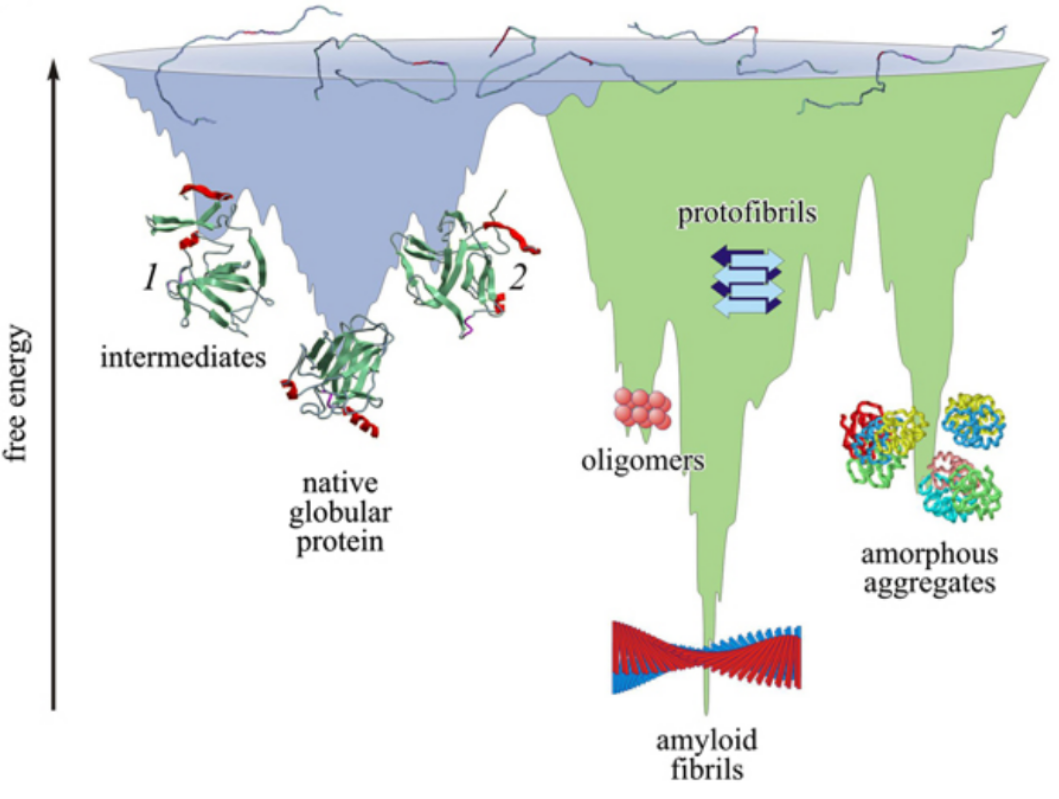
\includegraphics[width=0.7\textwidth]{img/globularEnLandscape.png} 
\centering
% 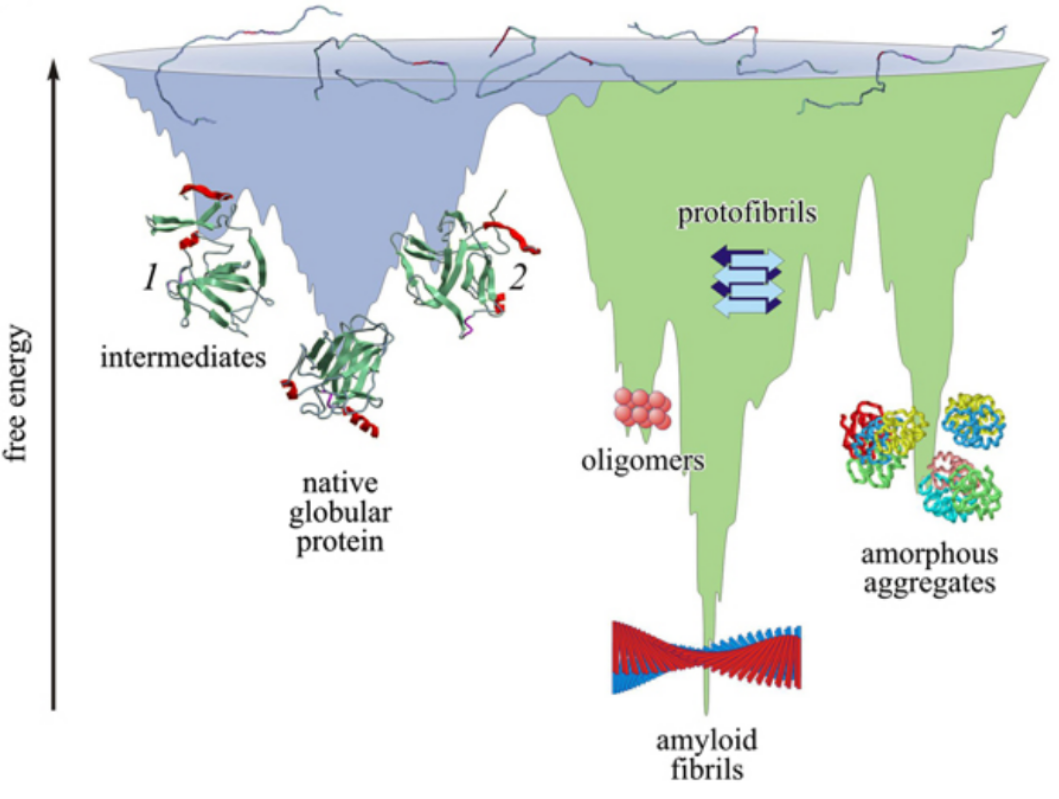
\includegraphics[width=0.7\textwidth]{img/globularEnLandscape.png} 
\caption{Perfil energetico de los estados de un polipeptido con estructura nativa globular. Figura extraida de \cite{turoverov2010protein}}
\label{globularFullEnLandscape}
\end{subfigure}

\begin{subfigure}[ht]{\linewidth}
\centering
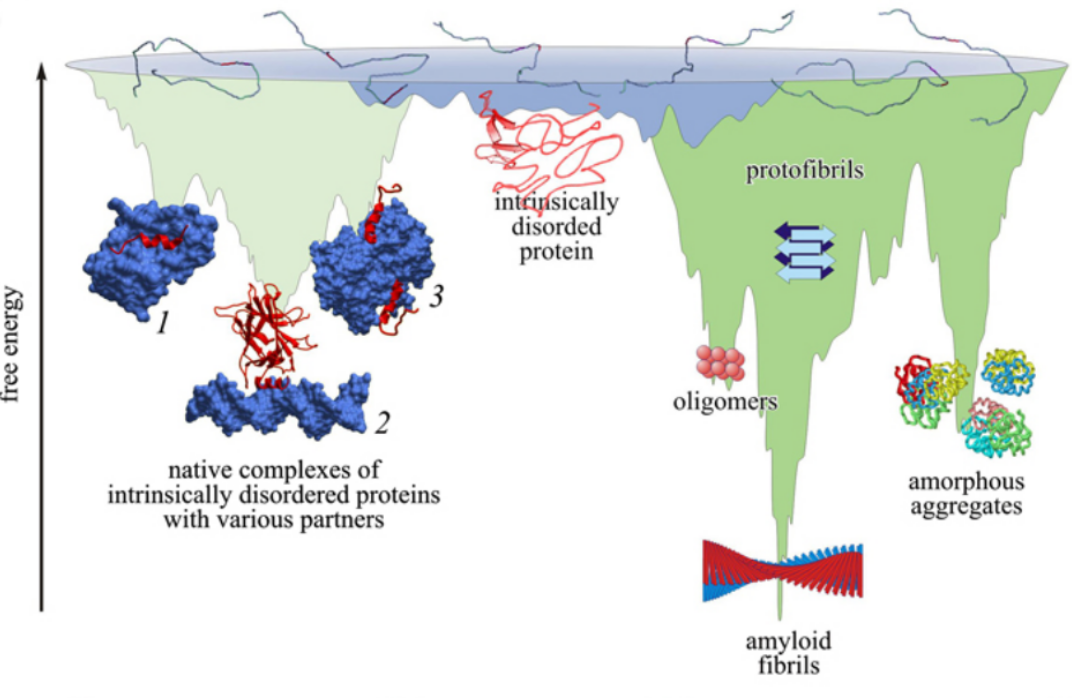
\includegraphics[width=0.7\textwidth]{img/idpEnLandscape.png} 
\caption{Perfil energetico de los estados de un polipeptido con estructura nativa desordenada. Figura extraida de \cite{turoverov2010protein}}
\label{idpFullEnLandscape}
\end{subfigure}
 \caption{Full energy landscape}
 \label{fullEnLandscape}
\end{figure}




% FACTORES EXTERNOS QUE AFECTAN LA AGREGACION
Además de las propiedades que se analizaron sobre la secuencia primaria, es importante destacar factores externos a la secuencia que pueden afectar la formación de agregados.
Los determinantes extrínsecos mas relevantes son el pH y la fuerza iónica de la solución, junto con la temperatura del sistema.
Estas variables pueden afectar tanto la cinética como las propiedades termodinámicas de los diferentes estados e intercambios entre estos.
Estas propiedades afectan a todos los estados posibles aunque en este caso los mencionamos en el contexto de proceso de agregación.
% The most relevant extrinsic determinants are the pH and the ionic strength of the solution, together with the temperature of the system [34].
% These variables may affect both the kinetics and thermodynamics of aggregation into amyloid-like structures, and can, subsequently, influence the assembly and
% the macroscopic structure of the aggregated species, thus being important determinants of the polymorphism the aggregates of a given protein sequence may present.



% BARRERAS CINETICAS QUE IMPIDEN LA FORMACION DE AMYLLOIDS
% Importantly, the cooperative nature of protein structures
% means that virtually none of the polypeptide chain in individual molecules is locally unfolded, 
% and that virtually no
% molecules in an ensemble are globally unfolded, even
% though native proteins are only marginally stable relative
% to denatured ones under normal physiological conditions
Como se ve en la fig.\ref{fullEnLandscape}\textbf{(a)}, en condiciones normales, donde los proteínas se mantienen en sus estados plegados, 
la estabilidad de estos estados los mantiene separados mediante barreras cinéticas relativamente altas de la formación de agregados(que se muestran considerablemente mas estables).
% Provided that the native state is maintained under conditions where it remains folded, aggregation to amyloid fibrils will be resisted by
% the kinetic barrier associated with unfolding, even if the aggregated state is thermodynamically more stable.
Esto no es tan determinante para intermediarios del plegamiento(estados 1 y 2 en fig. \ref{fullEnLandscape}\textbf{(a)}) y para las conformaciones desplegadas(fig. \ref{fullEnLandscape}\textbf{(b)}), 
donde las barreras energéticas pueden no ser determinantes en el mantenimiento de los estados nativos en solución.
Teniendo en cuenta que, como vimos antes, existe una gran diversidad de estados conformacionales en la célula,que el estado totalmente ordenado es, quizás, solo una excepción, y además se sabe que los agregados pueden provocar un gran daño biológico,
es esperable que los sistemas biológicos hayan evolucionado distintos mecanismos para mantener la homeostasis de los estados nativos monoméricos.
Este es el tema central que se desarrolla en la próxima sección.




% 
% 
% 
% These observations, therefore, have led to the remarkable conclusion that,
% at the concentrations present in living systems,
% the native states may not always represent
% the absolute free energy minima of the corresponding polypeptide chains, the native form of a protein could in some cases simply be a metastable monomeric
% (or functionally oligomeric) state that is separated from
% its polymeric amyloid form by high kinetic barriers.
% As much evidence reveals that the amyloid state is
% very resistant to denaturants and proteases, and mechanically robust, such a state could represent, at least under
% some conditions, a highly structured alternative to the
% native state but one that under normal biological conditions, although not under some disease-associated ones,
% may be kinetically inaccessible. 
% Understanding such kinetic factors therefore becomes a major target for developing an understanding of the circumstances in which
% amyloid assemblies occur in living systems.
% 
% 
% 





% ESTO LO PUEDO AGREGAR PERO NO SE DONDE PONERLO, ME PARECE QUE ES MAS DE LO MISMO IGUAL
% 
% **************************************************
% CONCLUSION SOBRE ESTADOS CONFORMACIONALES  -------   NO SE DONDE PONER ESTO!!! 
% *******************************************************
% Es por esto que las propiedades conformacionales de una proteína quedan mejor definidas si se declara el conjunto de multiples estados accesibles por sus estructuras.
% A este continuo de conformaciones que pueden adoptar las proteinas individuales, se agregan distintos tipos de estados agregados, conformados a partir de uniones entre proteinas 
% en distintas conformaciones iniciales(conformaciones desestructuradas, intermedios o plegados).
% De acuerdo con esta forma de ver, esta accesibilidad estará dada por la estabilidad termodinámica de cada conformacion accesible y la cinética de interconversión entre estas.
% Estos requerimientos pueden indicar por ejemplo q ciertos estados altamente estables como puede ser las fibras amiloides no sean estados naturales comunes debido a los requerimientos cinéticos, a pesar de ser termodinamicamente estables.
% De acuerdo con esta forma de describir las posibles conformaciones de las proteinas, the various fates awaiting a polypeptide chain once it has been synthesized in the cell 
% will depend on the kinetics and thermodynamics of the various equilibria between di¡erent possible states.

% Las propiedades cinéticas y termodinámicas están dadas por el contexto celular (pH, iones, concentracion de proteinas, presencia de otras moleculas con las que interactúa, etc) y, 
% obviamente, por los posibles cambios que puede tener una proteina, ya sean mutaciones o modificaciones postraduccionales.
% Esta forma de ver las propiedades estructurales permite ver los origenes de los cambios conformacionales desde el punto de vista de las propiedades fisicoquimicas de las proteinas.
% If the stability or cooperativity of the native state of a protein is reduced, for example by a mutation, the population of non-native states will increase.
% Es importante destacar, entonces que, for a given polypeptide chain a chosen fate is not a final one, and a choice may be further modulated by environmental pressure. 
% Thus, intrinsically unstructured proteins may be forced to fold or misfold via modification of their environment (addition of natural binding partners, changes in properties of solvent and so on), 
% whereas a destabilizing environment may push a natively folded protein to the misfolding route. Alternatively, the presence of chaperones may reverse the misfolding route and effectively dissolve small aggregates
% To begin to understand the manner in which proteins either adopt and maintain the specific states that are needed to carry out given functions or instead misfold
% and form potentially pathogenic aggregates such as amyloid fibrils, it is important to investigate the nature and properties of the various states in which these molecules
% can be found. 
% It is also important to clarify how the conversion of proteins into the amyloid state(o cualquier estado no funcional) is generally avoided in living systems.  
% *****************************************************************************
%ESTO ES LO QUE SE ESTUDIA A CONTINUACION  !!!!!!!!!!!!!!!!!!!!!!!!!!!!!!!!!!!!!!!!!!!!!!!!!!!!!!!!!!!!!!!!!********************
% 




















% EL PROCESO Y LA CINETICA DE LA FORMACION DE FIBRAS AMYILOIDS

% REF:  Protein aggregation: Mechnisms and functional consequences
% Amyloid fibrillogenesis is usually modelled as a nucleation-elongation polymerization process, which reaction rate depends on the protein concentration and can be accelerated 
% by the addition of homologous pre-aggregated polypeptides that act as seeds/templates promoting the transition from the soluble to the aggregated state
% According to this simplified model, amyloid aggregation can be divided in three main phases: 
% (1) The thermodynamically dis-
% favoured lag phase where the soluble species (usually monomers)
% associate to form nuclei, a poorly characterized state which for-
% mation influences the overall kinetics of the amyloid reaction. (2)
% The population of these transient assemblies triggers the poly-
% merization and fibril growth at the so-called exponential phase.
% (3) Finally, the exhaustion of monomers leads to the saturation
% phase where no more soluble species can associate to the ends of
% preformed fibrils and fibril maturation occurs, usually by lateral
% association of fibrils




























% 
% 
% 
% ***********************************************************
% CON LOS PROXIMOS PARRAFOS ARMAR UNA
% CONCLUSION GENERAL SOBRE TODOS LOS ESTADOS DE AGREGACION
% ************************************************************
% 
% 


% ACA DIGO QUE LAS FIBRAS AMILOIDES NO SON LA UNICA ESTRUCTURA PRODUCTO DE MISFOLDING
% 
% % PUEDO APROVECHAR ESTE PARRAFO PARA EXTENDER LA IDEA QUE LOS AGREGADOS NO SON NI 1 NI 2 Y QUE PUEDE HABER UNA GRAN CANTIDAD DE FORMAS EN LAS QUE SE AGREGAN LAS PROETEINAS
% En \cite{narhi2012classification} se estudian distintas formas de clasificación de agregados de proteínas:
% Protein aggregation is a complicated phenomenon,
% which is sensitive to solvent conditions, sample his-
% tory, protein sequence, and so on. Our ability to un-
% derstand aggregation will depend on the identifica-
% tion of patterns within this vast parameter space. It
% is our hope that these patterns will be more appar-
% ent with a more precise naming scheme. We propose
% using five categories: size, reversibility/dissociability,
% conformation, chemical modification, and morphol-
% ogy, to consistently describe protein aggregates.


% De todos los posibles estados de agregación, nos centramos en la formación de fibras amiloides porque....
% % Esto esta en \cite{knowles2014amyloid}
% The amyloid state, however, is relevant not only in
% the context of disease, but also because its very existence
% challenges in many ways our current understanding of the
% nature, structure and evolution of the functional states of
% proteins 26–30 . From a wide range of in vitro experiments on
% peptides and proteins we now know that the formation of
% amyloid structures is not a rare phenomenon associated
% with a small number of diseases but rather that it reflects a
% well-defined structural form of the protein that is an alter-
% native to the native state — a form that may in principle be
% adopted by many, if not all, polypeptide sequences









% MERGEAR ESTE PARRAFO CON EL QUE SIGUE, ARMANDO UNA CONCLUSION

% Although the data presented above were mostly devoted to a consideration of 
% protein fibrillation, the process of amyloid fibril formation does not represent the only misfolding route. 
% in fact, contrary to the process of productive protein 
% folding leading to the appearance of a rigid conformation with the specific 
% function, the end products of misfolding may have a different appearance. The 
% morphology of these end products depends on the particular experimental 
% conditions, and misfolded product may appear as soluble oligomers, amorphous aggregates, or amyloid-like fibrils. 
% any of these three species could be 
% cytotoxic, thus giving rise to the development of pathological conditions. 
% The reason for such a morphological difference is potentially connected with the diversity of the partially folded intermediates favoring protein self-association. 
% In fact, multiple environmental factors, such as point mutations, decrease in pH, increase in temperature, the presence of small organic molecules or metal ions, and other charged molecules, might induce structural rearrangements within a protein molecule, shifting equilirium toward the partially folded conformation(s). As different factors may stabilize slightly different partially folded intermediates, the formation of morphologically
% different aggregates is expected.













































\subsubsection{Mecanismos naturales de proteostasis} \label{proteostasis}

%  En \cite{balch2008adapting} se hace un desarrollo bastante completoo de los mecanismos de homeostasis

El estado ``normal'' de la célula se caracteriza por un fino balance entre la gran variedad de diferentes estados que las proteinas puede poblar y que hemos desarrollado a lo largo de las secciones previas.
A menos que se mantengan bajo control, las perturbaciones a este estado pueden llevar a efectos perjudiciales para la célula o el sistema. 

% CUALES SON LOS ESTADOS QUE HAY QUE EVITAR Y POR QUE?? 
% El plegamiento correcto de las proteínas para alcanzar su estado nativo es una gran parte de este balance y distintas perturbaciones pueden provocar el aumento de poblaciones en estados intermedios o \textit{misfolded}.
Las consecuencias obvias de aumentar la población de estos estados son la formación de agregados proteicos, pérdida de funcionalidades en las proteínas y aumento de funciones/componentes tóxicos o perjudiciales.
% In  order  for  any  biological  system  to  function  effectively,  it  is essential to avoid the inherent tendency of proteins to aggregate and form potentially harmful deposits.
El balance correcto entre todas estas condiciones está regulado a traves del proceso de proteostasis.
La proteostasis se refiere a controlar la concentracion, conformación, interacciones y localización de las proteínas individuales que hacen al proteoma readaptando la dinámica de la célula, 
generalmente a partir de cambios transcripcionales y traduccionales.
La proteostasis es afectada por la química intrínseca del proceso de plegamiento/desplegamiento de las proteínas y por una gran cantidad de redes de interacción y balance entre rutas biológicas que afectan a la síntesis, plegamiento, 
trafico, agregación y desagregación de proteínas.
% Proteostasis refers to controlling the concentration, conformation, binding interactions (quaternary structure), and location of individual proteins 
% making up the proteome by readapting the innate biology of the cell, 
% often through transcriptional and translational changes.
% The protein components of eukaryotic cells face acute and chronic challenges to their integrity. Eukaryotic protein homeostasis, or proteostasis, enables healthy cell and organismal development and aging and protects against disease
% Los mecanismos dentro del proceso de proteostasis permiten successful organismal development and aging in the face of constant intrinsic and environmental challenges %previniendo el desarrollo de enfernedades.


La naturaleza a desarrollado mecanismos muy sofisticados para regular efectivamente los estados de las proteínas en las celulas y prevenir efectos peligrosos de los desbalances.
La idea es que, entonces, ninguna proteína realmente está actuando de forma aislada sino que esta siendo ``observada'' a través de distintos mecanismos celulares. 
Esta maquinaria celular es suficientemente robusta como para tolerar desbalances considerables.
Obviamente, cualquier situación que afecta a estos mecanismos de protección contribuye al posible desarrollo de estados desbalanceados.
% Nature developed very sophisticated protection mechanisms (chaperones, proteasome, etc.) for the effective regulation of the folding process, y por lo tanto prevenir las peligrosas consecuencias de misfolding. 
% In other words, in the cell, any given protein is not acting in the isolation, is never alone and is constantly "watched" by the protective machinery. This machinery is rather robust and can
% tolerate significant loads. Obviously, factors that affect these protective mechanisms will contribute to the probability of disease development
Entre los mecanismos mas conocidos se encuentran las chaperonas, elementos escenciales de la maquinaria que controla la calidad de las proteínas.
En conjunto, las chaperonas moleculares controlan la translocación y el proceso de plegamiento de los polipéptidos nascientes, además de el replegamiento y degradación de proteínas incorrectamente plegadas, 
y la activación de un amplio rango de proteínas clientes de esta maquinaria.
% Molecular chaperones are essential elements of the protein quality control machinery that governs translocation and
% folding of nascent polypeptides, refolding and degradation of misfolded proteins, and activation of a wide range of client
% proteins
% that  the aggregation  process  is  generally   initiated  from  partially  or completely  unfolded  forms  of  the  peptides  and  proteins,
% por lo tanto, que las chaperonas no solo ayudan a la perdida de funcionalidad por plegamientos incorrectos sino tambien a la exposición de regiones secuenciales que puedan iniciar un proceso de agregación.

% MECANISMOS CELULARES DE PREVENSION AGREGADOS

A partir de lo que se dijo en la seccion anterior sabemos que el proceso de agregación comienza, generalmente, a partir de estados total o parcialmente desplegados,
por lo tanto, la prevención de errores en el plegamiento no sólo ayuda a evitar la pérdida de funcionalidad directa de las proteínas, sino también a la exposición de regiones secuenciales que puedan aumentar la tendencia a la agregación. 
La ocurrencia de un proceso de agregación de proteínas es una situación grave y existen una gran cantidad de mecanismos celulares que ayudan a prevenir la agregación.
En \cite{gsponer2012cellular} se demuestra que, por ejemplo, las proteínas propensas a formar agregados estan controladas mediante transcripción, traducción y degradación diferencial, en comparación con proteínas no propensas.
% aggregation-prone proteins are subject to differential transcriptional, translational, and degradation control compared to nonaggregation-prone proteins, which leads to their decreased
% synthesis, low abundance, and high turnover. 


Las diferencias estructurales vistas entre los distintos estados de agregación tambien se ven reflejada en diferencias biológicas. 
Esta segregación resulta en un tratamiento distinto por parte de los mecanismos encargados de la proteostasis.
Mientras que las proteinas en estados \textit{misfolded} y los agregados no estructurados se acumulan en el espacio perinuclear para luego ser degradados por el sistema del proteasoma,
los agregados amiloides preferentemente se acumulan en inclusiones perivacuolares y son degradados mediante el autofagosoma.
% Whereas misfolded and aggregated proteins are found in perinuclear locations and are generally degraded by the 
% proteasomal system, amyloids preferentially accumulate in perivacuolar inclusions, where they are degraded by the autophagosome.
% A reduced affinity of amyloids for the protein quality control system is probably also at the root of their higher toxicity 11 as artificial overexpression of chaperones
% usually leads to decreased toxicity and removal of amyloids from he cell.




% PROPIEDADES INTRINSECAS DE LAS PROTEINAS
Como los estados plegados pueden ser metaestables, y pueden existir estados agregados termodinámicamente más estables, las secuencias de las proteínas también han evolucionado para mantener su solubilidad \textit{in-vivo}
y evitar la conversión en estados agregados no funcionales.
% Como se vio en las secciones previas, as proteins in their functional forms can be thermodynamically and chemically metastable, mechanisms have evolved to maintain their solubility in vivo for prolonged periods of
% time and to avoid their conversion into non-functional amyloid states.
Es decir, además de los maquinaria dinámica que se encuentran en la célula y que se adaptan a las señales de la situación celular, existen propiedades evolutivas para mantener estados de proeostasis.
% esto esta en \cite{knowles2014amyloid}

Por ejemplo, un análisis de diversas fibrillas amiloides sugiere que este tipo de estructuras es propenso a volverse termodinámicamente inestable con respecto a estados monoméricos nativos(e incluso con respecto a estados desestructurados)
cuando las cadenas polipeptídicas tienen mas de aprox. 150 residuos, debido a restricciones topolígicas asociadas con el empaquetamiento de largas cadenas en el núcleo de la fibrilla\cite{baldwin2011metastability}.
La evolución parece haber explotado esta característica al desarrollar proteínas con un promedio de 300-500 residuos para minimizar el riesgo de formación de estos agregados.
% An analysis of a series of amyloid fibrils suggests that these types of structure are likely to become thermodynamically unstable relative to globular native structures, and indeed even relative to unstructured states, for
% polypeptide chains of more than ~150 residues because of the topological constraints that are associated with the
% packing of a long polypeptide chain into the fibril core 
% Biology may have exploited this feature by evolving proteins with 300-500 residues on average to minimize the risk of amyloid formation. 
Entre las diversas evidencias que apoyan esta idea se encuentra que los depósitos amiloides encontrados en situaciones de enfermedades 
están formados generalmente de péptidos y proteinas de corta longitud o, como se vio en la figura \ref{aggregationDiagram}, también pueden formarse a partir de fragmentos de la proteólisis de proteinas más grandes.
En \cite{knowles2014amyloid} se muestran otras propiedades intrínsecas de las secuencias para evitar los estados agregados. 
Algunas de estas son:
\begin{itemize}
 \item Las regiones propensas a agregación estan localizadas generalmente en el núcleo hidrofóbico de proteínas plegadas o como parte de la superficie que une distintas proteínas adoptando una estructura cuaternaria.
 Esto impide que estas regiones se encuentren en la superficie expuesta al solvente en el medio celular, impidiendo que puedan formar contactos anormales en el estado plegado correcto. 
%  APRs are usually located within or substantially take part in the hydrophobic cores of the native state of proteins [39] and also frequently map to protein-protein interaction surfaces of protein adopting
% a stable quaternary structure [40, 41], which prevents APRs from establishing aberrant intermolecular contacts

\item Además de su ubicación, se encontró que los segmentos propensos a agregación también poseen contextos ricos en residuos cargados cuya función, se cree, podría ser la de impedir interacciones en el caso que 
estos segmentos quedaran expuestos.
% The examination of APRs in the context of entire proteins has also revealed how these stretches are usually flanked by charged residues (Asp, Glu, Lys, Arg), whose
% function would be to hamper intermolecular interactions between APRs in the event they become exposed by providing repulsive charge, or by residues acting as $\beta$-sheetbreakers, like Pro


\end{itemize}


% 
% As aggregation cannot be completely eliminated, because of structural constraints from the native state, aggregation is further contained by placing not only charged residues but also prolines and 
% glycines at the flanks of aggregating sequence segments. These effectively act as gatekeeper residues, 
% opposing aggregation and thereby promoting the native folding reaction. It has also been reported on several occasions that the introduction of charged residues, prolines or glycines in aggregation-prone sequences reduces aggregation.
% The aggregation-opposing properties of proline and glycine originate primarily from their
% structure-breaking properties. Identically charged residues are also very effective at opposing aggregation, because of the huge repulsive force generated upon self-assembly.




% IDPs play a central role in many cellular processes, as their disordered nature provides them with the ability to bind many partners, thereby regulating many biochemical
% processes. Because of this central role, the malfunction of IDPs can disrupt proper cellular function and lead to disease.

% ACA EXPLICO POR QUE LAS IDPs NO TIENEN TANTA TENDENCIA A FORMAR AGREGADOS
% YA PUSE ALGO DE ESTO EN LA SECCION ANTERIOR, NO SE SI ES NECESARIO AGREGAR MAS
% In contrast to the globular proteins, which have to unfold prior to aggregation, IDPs are always ready for intermolecular interactions. 
% An unbound fragment of an IDP possesses a strong ability to interact, and therefore can bind either to natural partners forming native complexes or to similar molecules forming various aggregates. 
% This raises the question of why IDPs do not always form aggregates in the norm. One of the potential answers is the fact that inside the cell, the IDPs typically form complexes with natural partners.
% Los mecanismos de proteccion (chaperonas, proteasoma, etc) tienen una gran capacidad para mantener la solubilidad de proteinas.
% Además, based on the analysis of the IDP amino acid composition, it would be clearly a mistake to assume that an averaged IDP possesses higher propensity towards aggregation than an averaged ordered
% protein. In fact, many IDPs contain large number of charged and polar residues. In addition to the hydrophobic interactions, the net charge is one of the major factors determining aggregation behavior of a protein.
% 
% En \cite{linding2004comparative} se hace un estudio interesante de comparación entre un set de proteinas que adoptan estructuras globulares y otro que experimentalmente se sabe que son IDPs.
% % Se hace el analisis usando TANGO




% PREVENCION DE AGREGACION EN FOLDED PROTEINS
% the normal folding process may pass through
% partially folded states on the route to the fully native state,
% but the aggregation of these species will be minimized by
% the presence of molecular chaperones. In addition, if the
% protein is able to fold rapidly, any partially folded species
% will have a short lifetime, reducing the probability of inter-
% molecular interactions occurring. Moreover, once folded,
% the native state is generally a highly compact structure
% that conceals the polypeptide main chain within its
% interior. Such a state is protected from aggregation except
% through the interactions of surface side chains (as is the
% case, for example, in protein crystals) and is unable to
% form the strong intermolecular hydrogen bonds associated
% with the polypeptide backbone. 














































































\subsection{Características/elementos funcionales}
\label{functionalLandscape}


% PARADIGMA ESTRUCTURA-FUNCION TRADICIONAL 
El paradigma estructura-función original afirmaba que la función específica de una proteína está determinada por su estructura tridimensional, la cual es única y rígida. 
% The structure-function paradigm claims that a specific function of a protein is determined by its unique and rigid three-dimensional (3D) structure. 
% Thus, following its biosynthesis on the ribosome, a protein must fold to a native, defined 3D structure to be functional. 
% One of the bestunderstood functions of proteins is catalysis (i.e., enzymatic activity), which attracted much attention in the early days of protein science and led to the elaboration of the “lock and key” model by Fisher. 
% En este caso(enzimas) la proteina provee un scaffold para el sitio activo, 
% Central to this model is the notion that the correct shape of the substrate can fit into the active site of the enzyme for enabling an efficient and specific catalysis,
El origen de este paradigma es el modelo de llave-cerradura propuesto por Emil Fisher el 1894. E
l modelo nace de la necesidad por explicar la especificidad encontrada en el funcionamiento de diversas enzimas similares por sus correspondientes sustratos. 
% The primary origin of this structure-function paradigm is the “lock and key” hypothesis formulated in 1894 by Emil Fischer to explain the astonishing specificity of the enzymatic hydrolysis of glucoside multimers by different types
% of similar enzymes. 
La hipótesis utilizada para explicar esto era que la estructura de la proteína(en este caso la enzima) era perfectamente complementaria a la del sustrato correspondiente, en un sistema similar al de una llave en una cerradura.
Este paradigma extiende los conocimientos vistos previamente acerca de que la secuencia de la proteína tiene codificada la información necesaria para plegarse espontáneamente luego de ser sintetizada en la célula,
alcanzando esta estructura nativa asociada a la función.
Por un largo período de tiempo, entonces, el modelo de llave-cerradura y el paradigma asociado de secuencia-estructura-función se mantuvieron como teorías aceptadas, confirmadas continuamente por la
gran diversidad de estructuras que se resolvieron mediante difracción con rayos X. 
% For a long period of time, the validity of “lock and key” model and its associated sequence-structure-function paradigm was unquestioned, especially after the crystal structures of proteins started to be solved by X-ray diffraction
% Este paradigma se deriva de los primeros avances en el estudio de estructuras de proteinas. 
% Over the past century evidence steadily accumulated that a well-defined structure is the prerequisite of protein function.
% Basic biology and biochemistry textbooks that explain biological phenomena at the molecular level exquisitely rely on this notion, the ‘structure–function paradigm’.
La capacidad de asociar una estructura única, encontrada en el cristal, con la función observada de la proteína en solución reforzaba la idea de una estructura estática asociada a las proteínas
% The explanatory power of these 3-D structures continued to reinforce the static view of protein

% Throughout the 20th century, tens of thousands of structures have been solved and deposited in the Protein Data Bank (PDB), supporting again the necessity of a 3-D structure for functionality.
% that remained unquestioned.
Contrario a este modelo, en 1894 Koshlan sugiere el modelo de encaje inducido, basado en observaciones de enzimas que podían aceptar 
ligandos con diferentes estructuras y, por lo tanto, la proteína debía poseer cierta flexibilidad que le permitiera esta función.
% In contrast to this view, already in 1958 Koshland suggested the “induced-fit” model based on the observations that some enzymes could act on
% differently shaped substrates and hence a degree of flexibility is inevitable in function. 
Siguientes evidencias mostraron que esta flexibilidad era parte del mecanismo funcional y que podía implicar cambios conformacionales que van desde variaciones en rotámeros de las cadenas laterales hasta 
reordenamientos conformacionales muy relevantes(por ej. en proteínas alostéricas).
% A pesar de este reconocimiento de la dinamica para la funcion biologica, con 
Estas variaciones podian aún ser interpretadas dentro del modelo establecido por el paradigma estructura-función, el cual fue levemente adaptado.
El requerimiento necesario para que la proteína cumpla su función era, entonces, una estructura definida, aunque dinámica. 
% A well-folded, albeit dynamic, structure was thought to be the hallmark of protein function.

Como vimos en las secciones previas, las proteínas que se adaptan a esta descripción son proteínas plegadas y la estructura resultante que se observa de la cristalización es, en realidad, un promedio del ensamble de conformaciones.
% In general, such proteins are categorized as being "folded", and for these proteins(como se vio al inicio de la seccion de conformaciones), 
% structures determined by experimental methods such as X-ray crystallography correspond to the ensemble-averaged structures.
Como este ensemble de conformaciones es relativamente pequeño, con estructuras que varían poco respecto al promedio observado, es posible inferir información funcional a partir de la estructura promedio observada en la cristalización.
% Since the folded ensemble contains structures that have only small deviations from the ensemble average structure, 
% the ensemble average itself captures many important features of the protein's structure, and many insights into a protein's function can be garnered from this
% ensemble average structure
% Es decir, dado que en dominios globulares la estructura esta definida(podemos obtener un ensemble avarage) y esta asociada a la funcion que desarrolla la proteina, 
% esta estructura puede ser usada para clasificacion y para inferir la funcionalidad en nuevas proteinas.
% Estos dominios globulares pueden ser identificados y asociados a una funcion individual o a una funcion dentro de la funcion global de la proteina.
% PFAM, SCOP
% ACA IRIA LO DE SCOP
% Los análisis de estructuras existentes permiten la clasificación y anotación de éstas en bases de datos: ej. SCOP
El paradigma secuencia-estructura-función permite extender este concepto a la estructura primaria de la proteína.
Dado que la estructura asociada a la función debe ser mantenida evolutivamente para continuar cumpliendo la función, los requerimientos estructurales(y funcionales) imponen ciertas restricciones sobre la evolución de la secuencia.
Por lo tanto, la similitud secuencial también permite inferir propiedades funcionales. Esto facilita la anotación de elementos funcionales en secuencias nuevas, aún cuando no se conoce su estructura.
% Incluso cuando ....The sequences diverge, but the overall domain architecture remains the same.
% Particular domains and domain architectures are well conserved over the course of evolution. 

% HASTA ACA DEBERIA HABER DEFINIDO TODOS LO QUE RESPECTA A ESTRUCTURA-FUNCION EN DOMINIOS GLOBULARES






% ARRANCO CON IDPs



% ACA YA SE SOBREENTIENDE QUE LAS IDPs/IDRs PUEDEN TENER FUNCIONALIDADES
% Protein sequences in a genome can be viewed as modular because they are made up of combinations of structured and disordered regions.
% Proteins without IDRs are called structured proteins, and proteins with entirely disordered sequences that do not adopt any tertiary
% structure are referred to as intrinsically disordered proteins (IDPs). 
% The majority of eukaryotic proteins are made up of both structured and disordered regions, and both are important for the
% repertoire of functions that a protein can have in a variety of cellular contexts.

% Thus, functional regions in proteins can
% either be structured or disordered, and these need to be
% considered as two fundamental classes of functional building
% blocks of proteins

% Como se dijo en la introduccion, a little more than 10 years ago,however, such challenge to the almost dogmatic ‘structure–function paradigm’ was pure heresy due to the overwhelming evidence that structure determines function.

En las secciones anteriores se demostró que las proteínas completamente ordenadas eran sólo una parte de los estados posibles y que las conformaciones nativas de las proteinas pertenecen a un continuo mosaico estructural.
Debido a su amplio ensamble conformacional, el cual va más allá de una simple variación estructural, el modelo de encaje inducido no permitiría explicar su funcionamiento.
El paradigma estructura-función fuertemente establecido impedia aceptar, inicialmente, la idea de una función asociada a una IDR/IDP. 
% As it is often the case for new scientific concepts, the idea of structure-less functionality went through the stages of passive ignorance and active denial to scrupulous examination and enthusiastic acceptance
% Como parte de estos avances, en los ultimos años se han encontrado gran cantidad de proteinas que adoptan estructuras cuyas conformaciones son total o parcialmente desordenadas(segmentos globulares), soportando esta definicion, formalizada a principios de milenio. 
% the transition in paradigm was enforced by scattered experimental observations of disorder in a few dozen proteins. 
% Evidence added to that obtained by other techniques [mostly NMR and circular dichroism (CD)]..... and the evidence seems overwhelming now that structural disorder also exists in vivo and it is truly the native, 
% functional state of these proteins.
% Varios años de progresos en el área vencieron la sugestion y hoy en día la existencia de una gran variedad de funciones dependientes de IDRs/IDPs es parte del modelo actual de estructura-función.
% A decade of steady progress turned skepticism around and the suggestion that the native state of many proteins is intrinsically disordered (or, as originally termed, unstructured)
% is now integral to our general view of protein structure and function.
% una de las dudas que se tenia era si este estado conformacional existia solo in vitro y en realidad in-vivo lo que ocurria era que el crowding generaba el plegamiento

Como vimos antes, diversos estudios estructurales mostraron que este tipo de conformaciones existe realmente \textit{in-vivo} y representa el estado funcional de estas proteínas y,
dado que la habilidad para realizar su función biológica es lo que distingue al estado nativo, este conjunto de proteínas parcial o totalmente desordenadas debe ser considerada como entidades nativas. 
% As the main criterion of a native protein is its ability to perform a biological function, these partially or completely disordered proteins must be regarded as native entities.
% These proteins challenge(o mejor dicho destruyen) the “one sequence—one structure—one function” concept by demonstrating that the lack of stable tertiary and/or secondary structure
% does not preclude proteins from being biologically active
% Esta idea de proteínas desordenadas cumpliendo funciones biológicas desafía el paradigma(casi dogmático) de estructura-función.
Esto significa que el paradigma estructura-función previo, que implica la indispensable existencia de una estructura ordenada como requisito para una función efectiva, debe ser redefinido para incluir ese nuevo conjunto de entidades
\cite{wright1999intrinsically}.
% This means that the structure-function paradigm, which emphasizes that ordered 3D structures represent an indispensable prerequisite to effective protein functioning, should be redefined to include intrinsically unstructured proteins. 
De acuerdo a este nuevo paradigma, las proteínas nativas(o sus regiones funcionales) pueden existir en cualquiera de los estados conformacionales conocidos que se desarrollaron en las secciones previas.
% According to this redefined paradigm(disorder funcio),  native proteins (or their functional regions) can exist in any of the known conformational states.
En la figura \ref{stuctured-idp-functions} se muestra el paralelismo entre los paradigmas descritos y el proteoma resultante.
% El proteoma funcional esta compuesto, entonces, de un continuo de conformaciones que fall onto a structural continuum, from tightly folded single domains, to multidomain proteins that might have flexible or disordered regions, 
% to compact but disordered MOLTEN GLOBULES and, finally, to highly extended, heterogeneous unstructured states 

\begin{figure}[h!,centered]
\centering
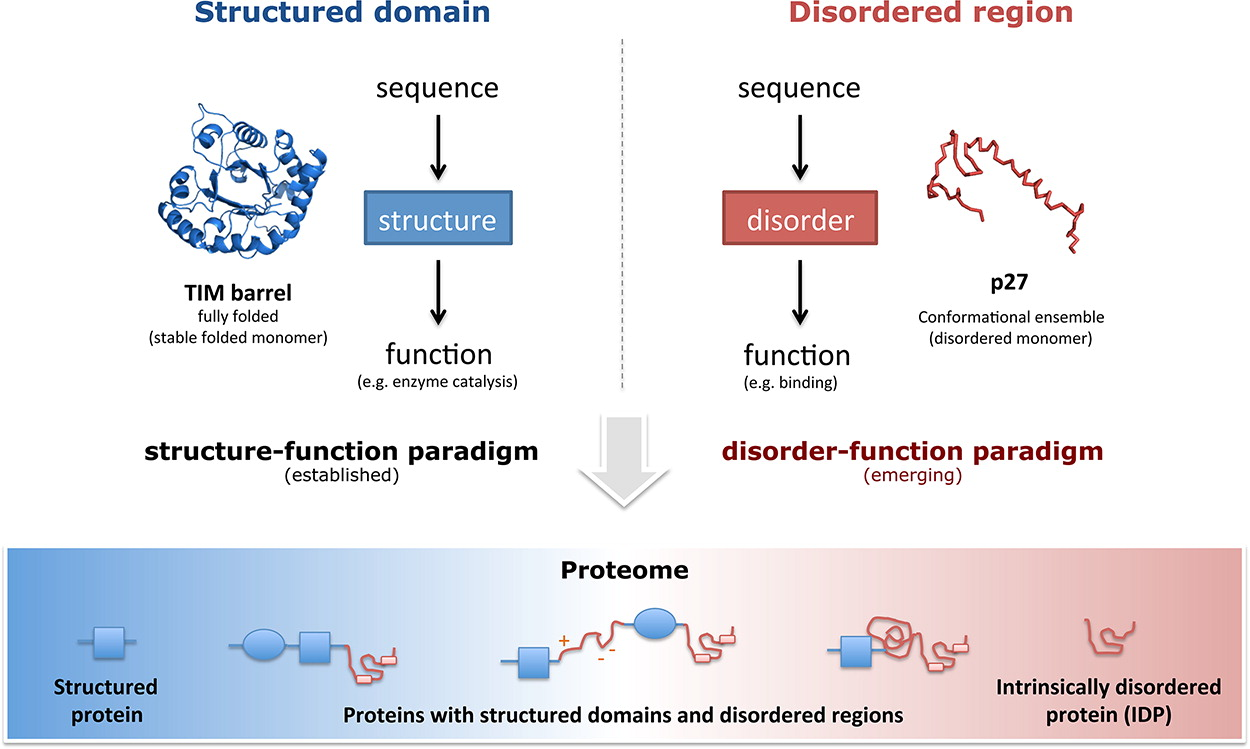
\includegraphics[width=0.9\textwidth]{img/structure-idp-function.jpeg} 
\caption{Paralelismo entre funcionalidad emergente de dominios plegados y de proteinas/regiones intrínsecamente desordenadas. Figura extraida de \cite{van2014classification}}
\label{stuctured-idp-functions}
\end{figure}




% PROTEIN QUARTET 
% PUEDO SACARLO COMPLETAMENTE
% 
% 
% To accommodate all these states in a functional framework, was elaborated the protein trinity hypothesis \cite{dunker2001protein} ,
% which posits that a native protein can be in one of three states -the ordered state, the collapsed-disordered (molten globule, MG) state, and the extended-disordered state (random coil, RC)- and that function can arise from any of the
% three states or from transitions between them. This model was subsequently expanded to include the premolten globule (PMG) state, which corresponds to an intermediate state between the RC and the MG. \ref{proteinQuartet} 
% % El modelo resultante actual esta compuesto de 4 estados\ref{proteinQuartet} que indican los posibles estados nativos(funcionales) de las proteinas.
% 
% 
% \begin{figure}[htbp]
% \centering
% 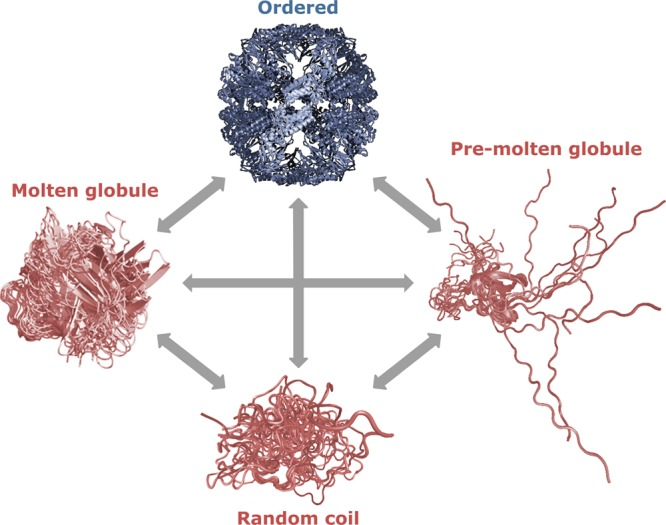
\includegraphics[width=0.7\textwidth]{img/proteinQuartet.jpg} 
% \caption{Protein quartet model of protein function. 
% Function can arise from four different conformations of the polypeptide chain, or from transitions between any of the states. Imagen extraída de \cite{uversky2002natively}}
% \label{proteinQuartet}
% \end{figure}







% PROPIEDADES Y MECANISMOS FUNCIONALES

El principal objetivo de todos los modelos y estudios estructurales en estas proteínas busca elucidar los tipos y modos funcionales subyacentes.
% The ultimate goal of the structural description of IDPs is to elucidate and rationalize the types and modes of functions they play.
La pregunta mas importante, entonces, es la función fisiológica que cumplen las IDRs/IDPs y como es su mecanismo funcional.
% The most important question of the field, therefore, is the physiological function and functional mode of IDPs/IDRs.
El estudio de las funcionalidades provistas por IDRs y IDPs se ve dificultada por las propiedades intrínsecas de estas proteinas:
Como se dijo antes, el paradigma inicial de secuencia-estructura-función provee una base para relacionar los conocimientos entre mediante métodos de análisis y anotaciones de secuencias estructuras y funciones.
Por el contrario, las proteínas dentro de este nuevo conjunto de IDPs se corresponden con un ensamble conformacional heterogéneo.
Dado que, entonces, no es posible obtener una estructura promedio representativa, es díficil obtener información relevante de la funcionalidad a partir del ensamble conformacional.
% By contrast, proteins within the more recently class of intrinsically disordered proteins (IDPs) sample dissimilar conformations during their biological lifetime, and therefore the corresponding structural
% ensembles are heterogeneous. 
% Given the vast number of structural states that are accessible to a disordered protein, the ensemble averaged structure for an IDP is typically not representative of any structure in 
% the ensemble itself and therefore has little utility for understanding that protein's function.
Lo que es más, dada la ausencia de restricciones estructurales, las secuencias de estas proteínas tienden a evolucionar más rapidamente que sus pares ordenados.
% Given the absence of structural constraints, IDRs tend to evolve more rapidly than protein domains that adopt defined structures. 
Como resultado, la identificacion de secuencias/regiones homólogas es considerablemente mas difícil.
% As a result, identifying homologous regions is harder for IDRs and IDPs than it is for structured domains.
% This complicates the transfer of information about function between homologues and thus the prediction of function of IDRs and IDPs.
Estas considereaciones manifiestan la necesidad de avanzar en el desarrollo de esquemas de clasificación específicos para este nuevo conjunto de proteínas, apuntando a mejorar la predicción funcional y la anotación.
% these considerations raise the need to devise a classification scheme specifically for disordered regions in proteins that may enhance
% the function prediction and annotation for this important class of protein segments.

% ESTO PODRIA PONER ALGO PERO NO HACE FALTA
% Aun cuando las propiedades a clasificar no sean discretas sino que formen un continuo de opciones, es util para explicar y entender mejor los conceptos.
% En secciones anteriores(mas precisamente en la seccion sobre propiedades conformacionales) se hicieron clasificaciones sobre la estructura global de la proteinas/regiones desordenadas, 
% ademas se clasificaron los mecanismos de binding en este tipo de proteinas como conformational selection and induced folding
% Especificamente se hablara aqui de clasificaciones sobre las funcionalidades y mecanismos funcionales provistos por estas proteinas.

Como parte de estos avances se han ensayado una gran diversidad de clasificaciones\cite{van2014classification}.
% Como parte de estos avances, para intentar dilucidar las funcionalidades de las IDPs y sus mecanismos asociados, se han intentado organizar y clasificar las funcionalidades provistas por estas 
% Como parte de estos avances para intentar dilucidar las funcionalidades de las IDPs y sus mecanismos asociados, se han intentado organizar y clasificar las funcionalidades provistas por estas \cite{van2014classification}.
En la figura \ref{proteinMechanisms} se ve una clasificación general bastante simplificada de los roles y mecanismos funcionales generalmente provistos por los distintos tipos de proteinas. 
En esta clasificacion de proteinas segun su rol general, se incluyen también los dominios/proteinas plegadas que mencionamos previamente.
La figura \ref{idpFunctions} detalla la clasificacion de funcionalidades y mecanismos funcionales específicos de IDPs/IDRs estimando las proporciones de cada funcionalidad.
Al parecer, de estas clasificaciones se puede ver que las funcionalidades en IDRs/IDPs emergen a partir del propio desorden o mediante mecanismos de reconocimiento molecular.

En el primero, el mecanismo subyacente de funcionamiento no implica adquirir estructura determinada, sino que depende directamente de la felxibilidad y plasticidad de la cadena carbonada(\textit{entropic chains}).
En este caso, las proteínas satisfacen un conjunto de requerimientos celulares únicos en los cuales la funcion a cumplir es una consecuencia directa del desorden intrínseco que poseen. 
Esta función, generalmente está asociada a secuencias linkers.

En el segundo caso, el mecanismo implica el plegamiento para adquirir una estructura ordenada al unirse al ligando.
% Apparent from the foregoing classification (Fig. \ref{proteinMechanisms}), IDP functions either directly stem from their disorder (((entropic chains where function involves no coupled binding and folding;
% rather it directly depends on the flexibility and the plasticity of the backbone . Occupy a unique structural and functional niche in which function is a direct consequence of intrinsic disorder))), 
% or from molecular recognition mechanisms , when they undergo induced folding (disorder-to-order transition) upon binding to a partner molecule. 
%IDPs often function via molecular recognition, when they bind partner molecules in, and induced folding process. 
Este mecanismo/estrategia de reconocimiento es básicamente diferente a la que adoptan los dominios plegados.
Mientras que estos últimos han evolucionado para dar una gran variedad de plegamientos diferentes que proveen reconocimientos especificos, 
en IDRs/IDPs el \textit{binding} es principalmente mediado por elementos(motivos) cortos de reconocimiento\cite{neduva2005systematic,fuxreiter2007local}.
% característicos por su naturaleza flexible
Este diferencia en el modo de reconocimiento les aporta una gran cantidad de ventajas\cite{gunasekaran2003extended,dyson2005intrinsically}.%REFERENCIA AL PAPER DE MECANISMOS FUNCIOMNALES DE IDPs
% This mode of binding is thought to confer many advantages 



\begin{figure}[h!,centered]
\centering
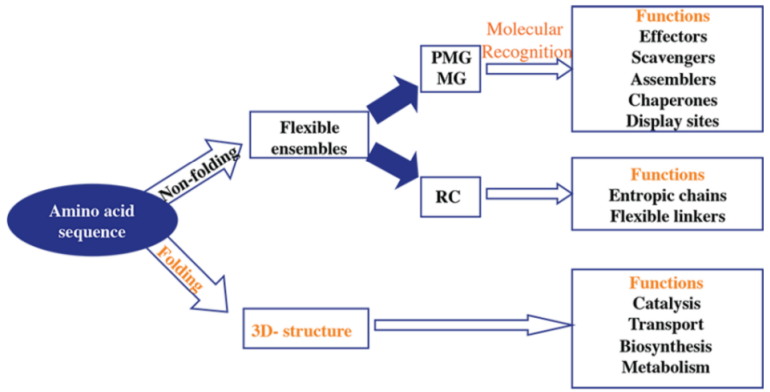
\includegraphics[width=0.9\textwidth]{img/proteinFunctionMechanisms.png} 
\caption{Distinctive properties of proteins: diversity and functional role. Figura extraida de \cite{habchi2014introducing} }
\label{proteinMechanisms}
\end{figure}





\begin{figure}[h!,centered]
\centering
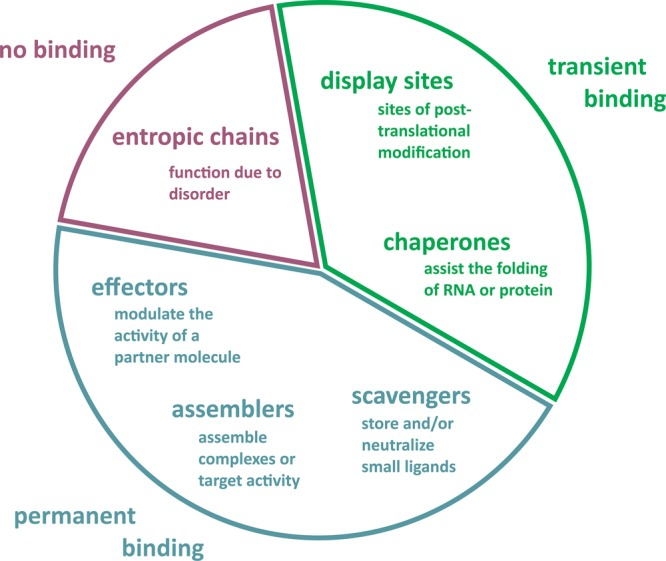
\includegraphics[width=0.7\textwidth]{img/idpFunctionMechanisms.jpg} 
\caption{Clasificación roles y mecanismos funcionales de IDPs/IDRs. Figura extraida de \cite{van2014classification}}
\label{idpFunctions}
\end{figure}




En la sección de propiedades conformacionales, se desarrollaron conceptos estructurales relacionados con elementos asociados al proceso de unión y plegamiento.
Ahi se describio que, generalmente, involucra regiones cortas de la secuencia con características anfipáticas y que denominamos elemento de reconocimiento(RE=recognition element). 
% only a part of an IDP, a specific recognition element, which is a relatively short amphipathic linear motif contained within long disordered sequence, is involved in the coupled folding and binding events
Ahora sabemos que son elementos funcionales fundamentales para la actividad de una gran cantidad de IDRs/IDPs, que tienen unos 10-70 aminoacidos de largo y pueden ser caracterizados a partir de sus propiedades conformacionales, 
% Es decir, ciertos elementos funcionales 
% En relacion a este concepto, nuevos conceptos han nacido para describir este tipo de entidades biologicas,
% Estos elementos funcionales, con  se denominan comunmente como Molecular Recognition Features (MoRFs)
\cite{mohan2006analysis,vacic2007characterization,oldfield2005coupled}.
% MoRFs are short segments in protein, which upon binding to their ligands undergo disorder-to-order transitions
Los REs(o MoREs por el nombre en inglés de Molecular Recognition Elements) pueden, a su vez, subclasificarse de acuerdo a las estructuras secundarias que adoptan en el complejo de unión. % bound state
Ademas, los dos modelos descritos antes sobre coupled folding and binding process in proteins permiten clasificar aun mas estos elementos(desde el punto de vista estructural), agregando el concepto de 
elementos estructurales preformados(PSEs)\cite{fuxreiter2004preformed}. 
Los PSEs se corresponden con el modelo de selección de conformaciones, es decir, son regiones intrínsecamente desordenadas que tienen tendencia a formar elementos estructurales transitivos, adquiriendo termporalmente estructuras secundarias.
Estos elementos pueden tener la capacidad potencial de servir como sitios de unión y quedar estabilizados en el complejo formado.
% PSEs are short disordered regions in IDPs, which have tendency for formation of transiently populated secondary structures, which may function as potential ligand binding sites. 
Esta clasificación no es totalmente excluyente ya que, como se dijo previamente, puede haber elementos que resulten de una combinacion de estos conceptos.
% Como se dijo, se definen como short, interaction-prone segments of protein disorder that undergo disorder-to-order transitions upon specific binding, 
% representing a specific class of intrinsically disordered regions that exhibit molecular recognition and binding functions.


% ACA CONECTO CON SLM
Mas allá de estas propiedades conformacionales que se estudiaron a lo largo de los años, el mecanismo subyacente a los motivos cortos de reconocimiento es, y ha sido durante mucho tiempo, estudiado desde el punto de vista 
de los patrones secuenciales que determinan las capacidades funcionales de éstos (interacciones o modificaciones enzimáticas). Estos elementos secuenciales se conocen como motivos lineales (o por sus siglas en inglés, LMs, ELMs, SLiMs o MiniMotifs)
\cite{davey2012attributes}. Estos motivos lineales se definen como modulos regulatorios encontrados en proteínas y que se caracterizan por presentar interfaces
de interacción muy compactas (los residuos determinantes de la afinidad y especificidad estan contenidos generalmente en unos 3-11 AAs contiguos).
% gulatory protein modules characterized by their compact interaction interfaces (the affinity and specificity determining residues are usually encoded between 3 and 11 contiguous amino acids (1)) 
% Sin embargo, molecular recognition by short recognition elements (motifs) can be -and has been historically- approached from the completely different direction of short sequence patterns determining functional interactions and enzymatic modification,
% also known as LMs, ELMs, short linear motifs (SLiMs), 125 or MiniMotifs  
% Es decir, LMs son elementos funcionales que, historicamente, fueron descritos desde el punto de vista secuencial. 
Como resultado de este número limitado de contactos para interacciones con ligandos, SLMs se unen con una afinidad relativa muy baja, lo que resulta en una ventaja considerable 
para participar en interacciones transientes, condicionales y  ajustables que son propias de los procesos regulatorios
% As a result of limited intermolecular contacts with their interaction partners, SLiMs bind with relatively low affinity (in the low-micromolar range), an advan-
% tageous attribute for use as transient, conditional and tunable interactions necessary for many regulatory processes. 
En términos de funcionalidad, se pueden clasificar los SLMs en dos grandes familias: los que actúan como sitios objetivo de modificaciones post-traduccionales(PTM), 
y los que funcionan como ligandos en la formación de complejos de interacción.
% the current census of SLiMs is split unequally between ligand motifs that mediate protein-protein interactions  and post-translational modification motifs, which are directly
% recognized and targeted for post-translational modification (PTM) by regulatory enzymes
% LO MISMO
% two major families: those that act as modification sites and those that act as ligands, with each having numerous subgroups
Dado que el conjunto de funcionalidades y propiedades estudiadas en relación a estos motivos lineales en la secuencia se corresponden en gran medida con las funcionalidades principales de IDRs/IDPs, en \cite{fuxreiter2007local} se
analizaron los perfiles conformacionales de proteínas que contienen instancias de éstos(no solo la conformación del segmento sino también el contexto), concluyendo que, efectivamente, 
suelen encontrarse formando parte de regiones IDRs y por lo tanto forman parte del conjunto de elementos funcionales característicos de IDRs/IDPs.
% Dado que el conjunto de funcionalidaddes que proveen los LMs se corresponde con el perfil que presentan las IDPs, se analizo el perfil conformacional de los LMs \cite{fuxreiter2007local}, 
Sin embargo, los SLMs se diferencian de los MoREs descritos previamente en que estos últimos dependen de un patrón de desorden en la secuencia(el cual puede ser obtenido con herramientas de predicción de desorden), 
mientras que los SLMs dependen de motivos secuenciales específicos.
% MoRFs differ from ELMs and SLiMs in not depending on a specific sequence motif, but rather upon a pattern in a disorder prediction output. 

Más adelante, luego de ver algunos detalles sobre los LMs, se volverá sobre este concepto y la relación con los otros elementos funcionales de las IDPs.
% Short linear motifs (SLiMs, LMs or MiniMotifs) and their enrichment in
% natively unstructured, or disordered, regions of proteins (2). 


El hecho que esten definidos por solo un pequeño segmento de AAs tiene consecuencias relevantes en aspectos biológicos de los SLM.
En particular, claramente resulta muy probable que estos aparezcan o desaparezcan mediante mutaciones. 
Dado que solo se necesitan un número muy limitado de mutaciones para que surgan, estos son propensos a la evolución convergente, lo que facilita la proliferación en distintos lugares del proteoma.
Esto resulta en una fuente de evolución para la red de interacciones ya que se generan interfaces \textit{de novo} en distintas proteínas.

Estas mismas características dinámicas de la secuencia los hace mas difíciles de estudiar que elementos funcionales mas restringidos evolutivamente como los dominios globulares.
Por lo tanto, a pesar de la disponibilidad de miles de secuencias de proteínas, el descubrimiento de motivos contenidos en estas es aún una tarea difícil.
% Their short length makes them difficult to detect using sequence comparison procedures that aid domain discovery. 
% They are typically discovered by difficult and time-consuming experimental procedures. 
% This usually involves first identifying a set of proteins sharing a common function (e.g., a common interaction partner or targeting within the cell), and then gradually delineating
% a short, common segment associated with this function through a variety of experimental techniques.

% SI ENCUENTRO REFERENCIA PARA ESTO LO AGREGO !!!
% Las propiedades de funcionalidad altamente dinamicas y la importancia biologica que tienen estos elementos hacen esperable que esten altamente regulados en la celula.






% *************************************************************
% ******    IDD  ********************
% ACA AGREGO OTRO ELEMENTO, LOS DOMINIOS ID, QUE PUEDEN SER OTRA CLASIFICACION
A pesar que las interacciones mediante SLMs suelen ser débiles, transitivas y, posiblemente, tener baja especificidad, pueden originarse interfaces mas especificas y de mayor afinidad si 
se obtiene cooperación de las regiones flanqueantes, si se combinan varios motivos cortos, o si se utilizan dominios desordenados con mayor longitud.
Es relevante decir que las regiones de unión en IDPs suelen corresponderse mas con dominios que con motivos cortos, teniendo longitudes que exceden los 20-30 residuos
\cite{tompa2009close,chen2006conservation,chen2006conservationB}.  
Además de esta longitud característica, tienen distintas propiedades que los distinguen como dominios:
Son estructuralmente y funcionalmente independientes dentro de la proteína, pueden ser más facilmente reconocibles mediante similitud secuencial debido a que sus secuencias están conservadas, 
y poseen al menos una función específica que los identifica.
Al poder distinguirlos como dominios intrínsecamente desordenados(IDDs) podemos clasificarlos, entonces, como una nueva clase de elementos funcionales independientes que pueden encontrarse dentro de IDPs.
Estos elementos tienen funciones muy diversas pero, generalmente, están involucrados en procesos de interacción con DNA, RNA u otras proteínas.



% DIFERENCIAS Y SIMILITUDES ENTRE SLiMs, MoREs e IDD
% 
A pesar que, como vimos, hay diferencias conceptuales entre motivos secuenciales y los MoREs, existen varias propiedades en común incluyendo la tendencia intrínseca al desorden 
y ser propensos a experimentar transiciones a estructuras ordenadas(\textit{folding-and-binding}). 
% Although there are differences in the definitions of linear motifs and MoRFs, they share many common features 72,163 including a tendency to undergo disorder-to-order transition (all
% MoRFs by definition and aprox. 60\% of LMs 48 ), an enrichment in IDRs (MoRFs by definition and aprox. 80\% of LMs are in IDRs 48,72 ), and a tendency to promote complex formation.
Varios estudios sugieren, entonces, que existen un gran solapamiento entre lo que normalmente definimos como motivos lineales y MoREs\cite{fuxreiter2007local,meszaros2012disordered}.
% Yet, interestingly, recent analysis suggests that linear motifs (LMs) (thus not differentiating between ELMs and SLiMs) show high overlap with MoRFs 
Dependiendo si la idea es definida/estudiada desde un punto de vista estructural o secuencial, entonces, un motivo lineal puede ser señalado como un MoRE o PSE.
Más allá de esto, a pesar de tener una longitud (al parecer) bastante mayor, los IDDs también poseen un solapamiento significativo con MoREs y motivos lineales.
% intrinsically disordered domains (IDDs) can also have significant overlap with MoRFs and linear motifs
Estos resultados parecen indicar que estos tres elementos funcionales pertenecen a estados de un mismo continuo de mecanismos de unión que pueden encontrarse en IDRs/IDPs.
% The overlap between linear motifs and MoRFs
% especially, but also IDDs, suggests that these functional features
% are different states in the same continuum of binding
% mechanisms involving disordered regions.

% Different concepts regarding short recognition elements have
% been extensively discussed in the literature. Indeed,
% depending
% on whether the idea is approached from a structural point of view
% or defined at the sequence level, a short motif could be denoted
% as a “molecular recognition element” (MoRE)/“molecular
% recognition feature” (MoRF) , a PSE, or “linear motif” (LM),
% respectively (LM is also denoted as “eukaryotic linear motif”
% (ELM) or “short linear motif” (SLiM)).


% ESTO ES LO MISMO, LO COMENTÉ PERO SE PUEDE RESCATAR ALGO
% Whereas LMs have been identified as short sequence motifs critical in recognition functions, primary contact sites, preformed structural elements and molecular recognition elments/features 
% have been approached from the direction of protein disorder, emphasizing recognition segments embedded in such regions. U
% nity of these concepts is underlined by the key role of a few specificity determinants in all these recognition elements, and also by their local preferences 
% for undergoing disorder-to-order transition upon molecular recognition, which might already
% be manifested prior to binding. 
% Apart from a minority of the cases when LMs are constituted of segments of ordered domains, these different concepts of short recognition elements express the same underlying physical and
% functional principles that provide a probably widespread solution to the dynamic control of protein-protein interaction networks.
% 





% AHORA QUE VIMOS TODO  INTENTAMOS HACER UNA CLASIFICACION!!!!!!!!!!
% 
% TAMBIEN ES UN POCO MAS DE LO MISMO, PERO PODRÍA SACAR ALGO
% Como se vio hasta acá, a pesar que la diferenciacion entre dominios y motivos es bastante clara, dentro de los motivos cortos de reconocimiento las diferencias no son tan claras
% Para entender mejor las funcionalidades, intentaremos ahora hacer una clasificacion de las functional features(elementos/modulos funcionales) que pueden encontrarse dentro de IDRs/IDP.
% % A measure that is often used to distinguish the different types of disordered binding modules is length.
% No perfect discriminatory properties can unambiguously distinguish the different types of binding elements, and the various interaction interfaces are characterized by a continuum of overlapping
% binding features. 
% Though disordered interaction modules encompass a continuous range of binding interfaces, they can be approximately split into three major classes of autonomous functional interfaces: 
% A three-category classification of protein interaction modules that have distinct functional, structural, and evolutionary dynamics has
% been proposed previously: globular domains, intrinsically disordered domains (IDDs), and SLiMs.  This classification
% defines a module as a minimal autonomous unit that, through interaction with another biomolecule, performs a regulatory,
% recognition, or enzymatic function. Each of these classes has a set of defining attributes that allows them to be discriminated
% from each other, and although exceptions exist for each category, these discriminatory attributes hold true for the
% majority of instances













































































\section{Ingeniería de proteínas}
% \label{proteinEngineering}


\subsection{Diseño de proteínas quiméricas}


Como producto de los avances logrados en las tecnologías asociadas al ADN recombinante, se ha desarrollado una nueva generación de proteínas compuestas por la unión de diferentes unidades estructurales y/o funcionales.
% Recent advances in protein engineering have come from creating multi-functional chimeric proteins containing modules from various proteins.
% As a product of recombinant DNA technology, fusion proteins have been developed as a class of novel biomolecules with multi-functional properties. 


% ACA PUEDO METER LA PARTE DE MODULARIDAD DE PROTEÍNAS
La idea de armar proteínas a partir de la unión de módulos no es algo nuevo.
Las proteínas naturales son usualmente modulares, conteniendo regiones definidas asociadas cada una con una subfunción específica.
% Proteins are usually modular, containing discrete regions each of which performs a different sub-function. 
Esta naturaleza modular provee muchas ventajas, principalmente la posibilidad de desarrollar funciones que requieren cooperación de distintos módulos y un incremento en la estabilidad de la estructura global.
% The modular nature of proteins has many advantages, providing increased stability and new cooperative functions.
Otra ventajas incluyen la protección de los metabolitos intermedios dentro de espacios inter-dominio, aumentando la eficiencia global y previniendo la liberación al medio de intermediarios inestables de la reacción.  
% Other advantages include the protection of intermediates within inter-domain clefts that may otherwise be unstable in aqueous environments 
% and the fixed stoichiometric ratio of enzymatic activity necessary for a sequential set of reactions
Desde el punto de vista evolutivo, la modularidad en las proteínas incrementa la capacidad evolutiva reduciendo las restricciones necesarias 
para la adaptación y permitiendo que módulos preexistentes puedan funcionar en nuevos contextos para nuevos usos.
% In terms of evolution, modularity increases evolvability by reducing constraints on adaptation and by allowing preexisting parts to function in new contexts for novel uses.
Estas diferencias en las propiedades da origen a diferentes definiciones del término dominio: 
Podemos definir a un dominio como una unidad evolutiva independiente que puede formar una proteína mono-dominio o formar parte de una multi-dominio. 
Esta unidad puede tener una función independiente o contribuir a la función global de una proteína multi-dominio coperando con el resto de las unidades.
Esta definición de dominio como unidad evolutiva es la que se usa como mecanismo de clasificación en la base de datos SCOP(Structural Classification of Proteins)\cite{murzin1995scop}. 
% We can define a protein domain as an independent, evolutionary unit that can form a single-domain protein or be part of one or more different multidomain proteins. The domain can either have an independent
% function or contribute to the function of a multidomain protein in cooperation with other domains. 
% The definition of a domain as an evolutionary unit is used in the Structural Classification of Proteins (SCOP) database \cite{murzin1995scop}
A diferencia de esto, en CATH\cite{orengo1997cath}, los dominios se definen basándose en conceptos puramente estructurales. 
De esta forma, los dominios pueden definirse como porciones de la secuencia de un polipéptido que pueden asumir una estructura tridimensional estable de forma independiente. 
% domains are domains are defined on a purely structural basis.
% De esta forma .........protein domains can be defined as segmented portions of a polypeptide sequence that assume stable three-dimensional structure.

Las distintas bases de datos permiten obtener, entonces, una gran cantidad de módulos estructurales y funcionales y gran 
parte del diseño de proteínas quiméricas se basa en utilizar estos conocimientos y anotaciones para crear nuevas proteínas con estructuras/funciones/propiedades combinadas.
Estas nuevas proteinas quiméricas(o de fusión), se utilizan de manera rutinaria para alcanzar distintos objetivos:

\begin{itemize}
 \item Creación de proteinas que combinan funciones de distintos dominios:
% En las secciones anteriores se describio como los dominios.... are considered (one of the most)the basic modules of protein structure, evolution and function.
% Por lo tanto, se conocen una gran cantidad de dominios..
Cómo se dijo en la sección anterior, se conocen una gran cantidad de dominios los cuales se encuentran anotados con una gran cantidad de funciones correspondientes.
% More than 7000 domains are known(citar Pfam), performing an enormous diversity of functions from catalysis during metabolism to cell–cell recognition in the immune system. 
La forma mas común de crear proteinas quimericas es, entonces, fusionar genéticamente dos o más dominios con subfunciones distintas, obteniendo una nueva funcionalidad global para la proteína.
% By genetically fusing two or more protein domains together, the fusion protein product may obtain many distinct functions derived from each of their component moieties.
\item Facilitar el estudio de interacciones proteina-proteina\cite{reddy2013linkers}: 
Tradicionamlente el estudio se hace expresando conjuntamente las dos proteinas que conforman el complejo.
Sin embargo, si la afinidad es muy baja, no es tan simple obtener el complejo formado.
La creación de una proteína quimérica que une a los dominios/proteínas que forman el complejo permite mantenerlas unidas mediante un linker.
La flexibilidad de esta secuencia linker debería permitir la correcta formación del complejo y, al estar unidas covalentemente, habrá una posibilidad mucho mayor de interacción.
El aumento en la estabilidad del complejo permite realizar los estudios biofísicos necesarios sobre éste.
% The characterization of protein–protein interactions is often required to gain an understanding of various biological processes. 
% Yet, the study of protein–protein interactions for many complexes is hampered when one or more partners of the complex are unfolded or unstable. 
% Traditionally, this problem has been addressed by the co-expression and/or copurification of both proteins. 
% However, for weakly interacting or unstable complexes, the co-expression and/or co-purification often results in a single pro-
% tein. 
% Protein engineering techniques were another
% option to address unfolded or unstable proteins,
% using a single polypeptide chain chimera to link the
% two binding partners via a flexible amino acid linker
% 13
% . With these chimeric proteins, it was then possible
% to maintain both the intramolecular and intermolec-
% ular protein–protein interactions, 14 and chimeric
% proteins have been used to generate stable, soluble
% binary complexes for structural studies, as well as
% functional dimers.
% Linking binding partners using an artificial
% linker will increase the proximity between the inter-
% acting partners and preserve the natural interaction.
% In cases where the interacting partners are not
% linked, it is possible that the binding partners might
% dissociate due to their low affinity and/or due to the
% crystallization conditions.
\item La unión de fragmentos de anticuerpos a enzimas o proteínas que permitan la detección de la unión es la base de las técnicas inmunoquímicas.
% \item Incrementar la expresión de proteínas.
\item La unión de segmentos de secuencia específica permite la purificación de proteínas a partir del lisado celular. 
% Facilitar la purificación de proteínas.
% Una de las aplicaciones mas interesantes es para ayudar al estudio estructurals de las intereacciones entre proteinas \cite{}.
% -In addition to structural studies of protein–protein interactions \cite{reddy2013linkers}.,
% \item a wide range of applications in the field of biotechnology have employed these fused proteins
% \item to explore protein-based biochemistry, such as to create artificial bifunctional enzymes and as tools for FRET analysis.

% They have also been widely applied for drug targeting, since proteins such as single chain antibodies or ligands for cell surface receptors can 
% specifically target a linked functional protein (e.g. toxin or cytokine) to a specific type of cells
\end{itemize}








% El diseño de nuevas proteinas quimericas requiere, obbviamente, de dominios a conjugar, los cuales normalmente se conocen ya que forman parte del experimento(o pueden buscarse mediante funcion en bases de datos como Pfam).
% Pero además, como se vió antes, la proteina modular tipica esta compuesta de independently folded globular domains that are separated by flexible linker regions, por lo que se require obtener este linker, 
% el cual debe conferir a los dominios la libertad suficiente para cumplir sus funciones sin restricciones.

La construcción de una proteína de fusión(quimérica) requiere de dos elementos indispensables: 
los dominios o proteínas a fusionar, y la secuencia linker que los va a unir.
La elección de los dominios/proteínas está fuertemente ligada al producto final que se desea obtener y, normalmente, se pueden obtener de forma directa.
% objetivo que se está buscando con la técnica experimental 
% The successful construction of a recombinant fusion protein requires two indispensable elements: 
% the component domains/proteins and the linkers.
% The choice of the component domains/proteins is based on the desired functions of the fusion protein product and, in most cases, is relatively straightforward. 
Por otro lado, la selección de un linker adecuado para unir los dominios/proteinas de acuerdo al objetivo que se busca puede ser un paso complicado y es generalmente ignorado cuando se piensa en el diseño de una proteína quimérica.
% On the other hand, the selection of a suitable linker to join the protein domains together can be complicated and is often neglected in the design of fusion proteins.
La unión directa de los dominios/proteínas o el uso de un linker inadecuado puede resultar en resultados indeseables, por ej. puede restringirse la capacidad de plegado de algun dominio globular, bajar el rendimiento de la proteína resultante o
disminución en la actividad biológica de alguno de los módulos.
La correcta selección, o mejor aún, el diseño racional de las secuencias linker para unir los módulos es un aspecto importante, aunque poco desarrollado, del diseño de proteínas quiméricas. 
% Direct fusion of functional domains without a linker may lead to many undesirable outcomes, 
% including misfolding of the fusion proteins [17], low yield in protein production [18], or impaired bioactivity [19, 20]. 
% Therefore, the selection or rational design of a linker to join fusion protein domains is an important, yet underexplored, area in recombinant fusion protein technology.

Esta falta de desarrollo en el tema se debe, quizás, a la falta de conocimiento sobre los factores estructurales que gobiernan la flexibilidad entre los dominios.
Este factor limita, claramente, el diseño \textit{de-novo} de proteínas quiméricas. Los conocimientos relevantes sobre este tema pueden aparecer a partir de la gran cantidad de secuencias que se disponen actualmente, los avances en 
la identificación de dominios y nuevas técnicas para obtener sus propiedades conformacionales a partir de la información secuncial.
% Despite many empirical surveys, very little is known about the structural factors that govern interdomain flexibility. 
% Such lack of knowledge is a limiting factor in de novo chimera design. Therefore, a number of recent studies focused on the structural principles governing the domain architecture and their assembly. 98–107.
% The emerging concepts, along with the bioinformatics tools that attempt to detect domains and their motions from sequence information alone, 108 may one day lead to a precise de novo engineering of interdomain flexibility, thereby helping
% achieve the desired functioning of synthetic chimeras.


% DISORDER vs FLEXIBILITY:
Para las arquitecturas más comunes, compuestas de dominios globulares unidos por linkers, la flexibilidad de esta secuencia linker es un requerimiento escencial.
Es relevante aclarar acá que, si bien los terminos desordenado y flexible pueden solaparse en algun punto, son términos distintos\cite{radivojac2004protein}
% Disorder and flexibility are often used synonymously, but the two terms are quite distinct\cite{radivojac2004protein}. 
% With regard to an ordered protein, flexibility refers to the magnitudes of the excursions of the atoms from their equilibrium positions.
Para una region desordenada, la variación en la flexibilidad se refiere a las diferencias en las velocidades de interconversión entre los diferentes estados miembro del ensamble estructural.
Una variedad de técnicas biofísicas, como por ej. NMR, han sido usadas para estudiar estos conceptos de flexibilidad.
% For a disordered region, variation in flexibility refers to differences in the speed of interconversion among the various members of the structural ensemble. 
% A variety of methods have been used to investigate the flexibilities of disordered regions and proteins, including NMR.
Análisis de estructuras mediante estas tecnicas muestran que el movimiento en la proteína que provoca los cambios conformacionales puede ocurrir tanto a nivel de residuos como a nivel de estructura secundaria o terciaria. 
% Analyses of structures(por ej. mediante X.ray diffraction) have shown that protein motion may occur due to conformational changes in individual 

% Control of structural flexibility is essential for the proper functioning of a large number of proteins and multiprotein complexes. 
% At the residue level, such flexibility occurs due to local relaxation of peptide bond angles whose cumulative effect may result in large 
% changes in the secondary, tertiary or quaternary structures of protein molecules. 
% Such flexibility, and its absence, most often depends on the nature of interdomain linkages formed by oligopeptides.


% residues or at the secondary, tertiary, or quaternary structural levels. 
% Lactate dehydrogenase, triose-phosphate isomerase, as well as hemoglobin 
% and related proteins are some of the earliest examples of proteins that showed conformational changes with important functional implications.

% 

Además de los analisis sobre las propiedades físicas asociadas a las arquitecturas modulares, el estudio de la diversidad de linkers encontrados en la naturaleza puede proveer información importante para entender los requerimientos
más importantes en el diseño de estas secuencias.
% Knowledge of natural linkers in multi-domain proteins is very helpful for the (rational??) design of empirical linkers in recombinant fusion proteins. 
Este es el tema de la próxima sección.






























\subsection{Secuencias linker naturales}


% El 'descubrimiento' de las regiones/secuencias linkers esta ligado a las teorias de structura-funcion(desarrolladas en la parte de conformacion) que se dieron durante casi 100 años
% En un principio se comenzo a pensar en una estructura rigida asociada a la proteina, luego se fueron revelendo propiedades dinamicas que le permitian cumplir la funcion. 
% Todo esto esta muy asociado a las tecnicas experimentales que se fueron desarrollando.
Como se dijo antes, la modularidad en proteínas naturales es algo muy común y existen muchisimos ejemplos de proteinas multidominio compuestas de dos o mas dominios funcionales unidas por linkers.
Estas secuencias linker sirven, principalmente para mantener unidos los distintos dominios, pero también proveen muchas otras funciones a la proteína como intervenires en las interacciones cooperativas entre los dominios o formar parte de la actividad biológoica de la proteína.
% These linker peptides serve to connect the protein moieties, and also provide many other functions, such as maintaining cooperative inter-domain interactions [21] or preserving biological activity [22]. 
% 
% Los primeros estudios de analisis (estructura y composicion) de secuencias linkers\cite{argos1990investigation} se comenzaron a hacer a partir del analisis estadistico de secuencias que podian ser clasificadas 
% como linkers a partir de las primeras estructuras de proteinas multidominio almacenadas en bases de datos.
% % Estos estudios estaban sesgados por todo el proceso historico de descubrimiento marcado por 
% Los resultados indicaban que la mayoria adquiría una conformación desplegada(tipo \textit{coil}) sin estructura secundaria. 
% % many studies of linker peptides in various protein families have come to the conclusion that linkers lack regular secondary structure (la mayoria se encontraba en estructuraas tipo coil), 
% % they display varying degrees of flexibility to match their particular biological purpose and are rich in Ala, Pro and charged residues
% Asi surgio la idea que los linkers eran secuencias cortas cuya unica funcion era proveer la conexion covalente, lo que estaba de acuerdo con el concepto de hinge-bending.
% Este concepto indicaba que la flexibilidad de estas regiones cortas dentro de un polipéptido permitía el suficiente movimiento a los dominios estructurales.
% % The concept of hinge-bending, whereby the relative flexibility of these short regions of the polypeptide chain allows significant movement of structural domains, gained widespread acceptance in
% % the 1980s and early 1990s, after evidence for conformational transitions in identical or homologous proteins became known.

% It was discovered that hinge regions are soft-linker regions of localized torsion angle changes in
% the polypeptide chain that allow the attached rigid
% domains to pivot. The rotation axes of these torsion
% angle changes are nearly parallel to the overall axis of
% rotation, so the local motion in the hinges can be
% directly related to the overall motion. A crucial feature
% of the hinge residues is that they have very few packing
% constraints on their main chain atoms.
% 


% A lo largo de los años los conocimientos sobre la composición y propiedades de estas secuencias ha ido cambiando, 
% a medida que mayor cantidad de estructuras se resolvian y mayor conocimiento se obtenia acerca de los dominios que componen 
% las proteinas. Tambien influyeron otras cosas como tecnicas biofisicas que permiten obtener información del ensamble conformacional en solución,
% o algoritmos para automatizar la identificación de los dominios y las secuencias que actúan como linker en una proteina.
% 

% Although the role of linker sequences is likely to be primarily topological, allowing distant parts of the polypeptide chain to interact with diverse partner sequences that might be far apart or close together, 
% linkers and unstructured tail sequences play quite specific roles in a number of systems.

% Hoy en día solo se puede decir que, a pesar que la funcionalidad topológica(actuan como espaciadores entre los dominios de una proteina) es probablemente la más importante,
% % Hoy en dia, solo se puede decir que los linkers naturales son secuencias que actuan como espaciadores entre los dominios de una proteina, de manera que se prevengan interacciones unfavourable between folding domains. 
% % Esto solo se puede decir acerca de su definicion, ya que 
% por encima de esto, existen distintas propiedades estructurales/funcionales que dependen de la función global de la proteína.


En \cite{argos1990investigation,george2002analysis} se encuentran los análisis mas detallados donde se estudian las propiedades generales de secuencias linkers naturales
En \cite{chen2013fusion} se revisan los resultados obtenidos en ambos con respecto a diversas propiedades como son longitud, hidrofobicidad, enriquecimiento de ciertos aminoacidos y estructura secundaria adoptada.
% properties of the natural linkers, such as length, hydrophobicity, amino acid residues, and secondary structure were compared and the results are summarized in
En cada proteina, la secuencia linker puede tener una estructura y una función que haya sido seleccionada para el mecanismo/localización/función de la proteina como un todo, 
y esta función del linker puede no ser solamente la unión covalente de dos dominios. 
% para proveer increased stability and new cooperative functions.
% Por ejemplo, algunos linkers can play an essential role in maintaining cooperative inter-domain interactions
De esta forma, es dificil hacer un analisis y una clasificación exhaustiva de todos los linkers.
% Si se pueden agrupar algunos segun distintas caracteristicas funcionales, estructurales, etc.
% En \cite{george2002analysis} se esboza una clasificación de los linkers de acuerdo al análisis de su estructura secundaria.
% Se dividen, así, en dos categorías: helicoidales y no helicoidales.
% Los linkers con estructuras de $\alpha$-hélice pueden tener funciones como, por ejemplo, actuar como espaciadores rígidos impidiendo interacciones no funcionales entre los dominios.
% Aunque no sea exhaustiva, esta clasificación permite ver diferencias en los linkers también a nivel de estructura que adquieren, existiendo linkers que, a través de una mayor rigidez, impiden . 

En general, se encontro que los linkers naturales adoptaban principalmente conformaciones desplegadas y tenían estructuras independientes sin interacciones con los dominios adyacentes.
Todas las propiedades analizadas(longitud, composición, hidrofobicidad y estructura secundaria.) resultaron importantes para alcanzar las funciones deseadas.
% Overall, natural linkers mainly adopted extended conformations, and had independent structures that did not interact with the adjacent protein domains. 
% Taken together, their length, composition, hydrophobicity, and secondary structure were all important to achieve the desirable functions.
En términos de estructura, por ejemplo, se encontraron tanto linkers flexibles como relativamente rígidos en muchas proteínas.
A través de una mayor rigidez, ciertos linkers pueden ayudar a reducir interacciones no funcionales entre los dominios que unen. 
Por otro lado, una estructura más flexible, como es usual para conformaciones extendidas, provee una mayor flexibilidad y libertad de movimiento a los dominios.
% Both flexible and relatively rigid peptide linkers are found in many multidomain proteins. 



% A FUTURO
Con el incremento del número de estructuras almacenadas en la PDB que ocurrió en los últimos años, sería posible realizar un estudio actualizado de las propiedades de los linkers naturales.
Además, sería interesante extender el número de propiedades analizadas agregando categorías asociadas a función y estructura de la proteína, e identificando la relación entre estas y las propiedades del linker.
% With the rapid increase of the number of protein structures deposited in the PDB database, an updated study of natural linkers could be conducted. 
% In addition to the properties analyzed in previous studies (e.g., amino acid composition, structure classification), 
% it would be interesting to categorize the multi-domain proteins by their functions and structures, and identify the relationship between them and the linker properties


% 
% 
% Based on From George and
% Heringa’s secondary structure analysis, linkers were grouped into two categories: helical and
% non-helical. The $\alpha$-helix was a rigid and stable structure, with intra-segment hydrogen bonds
% and a closely packed backbone [28]. Some $\alpha$-helical conformations form rapidly during
% folding [28], allowing the correct folding of connecting protein domains without non-native
% interactions with the linker. Linkers in an $\alpha$-helix structure might also serve as rigid spacers
% to effectively separate protein domains, and to reduce their unfavorable interactions.
% Therefore, this conformation was commonly adopted by many natural and empirical linkers
% (to be discussed later). On the other hand, without an inherent rigid structure, the non-helical
% linkers tended to be rich in Pro, which could increase the stiffness of the linker as mentioned
% previously [25]. As a result, non-helical linkers with Pro-rich sequence could exhibit
% relatively rigid structures and serve to reduce inter-domain interference.
% 
% 
% 
% Both flexible and relatively rigid peptide linkers are found in many multidomain proteins. 
% Linkers are thought to control favorable and unfavorable interactions between adjacent domains by means of variable softness
% furnished by their primary sequence. Large-scale structural heterogeneity of multidomain proteins
% and their complexes, facilitated by soft peptide linkers, is now seen as the norm rather than the
% exception. Biophysical discoveries as well as computational algorithms and databases have
% reshaped our understanding of the often spectacular biomolecular dynamics enabled by soft linkers.
% Absence of such motion, as in so-called molecular rulers, also has desirable functional effects in
% protein architecture.







% 
% 
% \subsubsection{Molecular rulers}
% These linkers are more defined by their ability to reliably predict and maintain end-to-end distances between attached domains. 
% Such structurally rigid peptides have been conjugated to molecules to serve a metric function.
% These linkers are rich in Proline. 
% Proline is common to many naturally derived interdomain linkers, and structural studies indicate that proline-rich sequences form relatively rigid extended structures to prevent unfavorable interactions between the domains.
% The probable reason why proline is favored over other residues in linking different domains is the inability of proline to donate hydrogen bonds or participate comfortably in any regular secondary structure conformation. This ensures a relatively rigid separation of the domains, thereby preventing unfavorable contacts between them.
% 
% Although short stretches of hard linker sequences are located between functionally relevant regions of protein structure, mutations within such sequences may have no effect on the function.  
% Such linkers are therefore necessary to keep the other amino acid interactions in register, but the nature of the side chain is often unimportant.
% 
% The observed natural tendency to form rigid linkers might also
% be related to avoiding proteolytic cleavage, as linkers are likely
% targets for protease degradation
% 
% Linker
% sequences vary greatly in length and composition, but
% many are rich in polar, uncharged amino acids (such as
% Ser, Thr, Gln and Asn), in the small residues Ala and Gly,
% and in Pro residues. Many of these residues tend to bias
% the polypeptide chain towards the polyproline-II region
% of the RAMACHANDRAN PLOT 27,28 .This means that such
% linkers, although flexible, have a propensity to be highly
% extended. Compositionally biased linker sequences of
% significant length are found mainly in eukaryotic pro-
% teins 1,29 , but short linker sequences of similar composi-
% tion, known as Q-linkers, are also found in a number of
% bacterial regulatory proteins 30 .
% In the absence of their targets, modular proteins
% often behave as ‘beads on a flexible string’, where the
% function of the linker is, primarily, to enable a relatively
% unhindered spatial search by the attached domains 31 .
% However, binding can induce structure formation in
% linkers, which can have significant functional conse-
% quences. For example, the sequence-specific binding of
% CYS HIS ZINC-FINGER PROTEINS to DNA causes the linker to
% fold, cap and thereby stabilize the preceding helix in the
% protein, and to orientate the next zinc finger correctly
% for binding in the major groove of DNA
% 
% 
% 
% %ESTUDIOS DE COMPOSICION, ETC....
% 









































  
  
  
  
  
  
  
  
  
  
  
\subsection{Diseño de linkers}
\label{linkerDesign}
A la hora de obtener un linker las propiedades estructurales suelen ser las más criticas.
La arquitectura típica creada, representada por dominios globulares unidos por secuencias linkers, se busca que éstos permitan 
mantener los dominios separados a la vez que se les da suficiente capacidad para moverse libremente como parte de su funcionalidad. 
Por lo tanto, la flexibilidad es el requerimiento mas importante.
% keeping domains apart while allowing them to move as part of their (catalytic?) function. 

Sin embargo, la flexibilidad no es todo. 
Por ej. una opción evidente seria usar linkers de solo Glicina ¿Por qué no usar siempre un linker puramente poli-G, adaptando solamente su longitud?
Desde los primeros estudios sobre linkers naturales \cite{argos1990investigation} se encontró que las proteinas naturales no usan(seleccionan) este tipo de secuencias.
Si bien esto no es concluyente para que no se usen, puede darnos un motivo para pensarlo dos veces.
En primer lugar, un péptido poli-G sería extremadamente inestable y por lo tanto podría actuar como una carga energética, estructural o interferir en procesos de catálisis de los dominios que une, 
especialmente si tiene una longitud excesiva.
% An all-Gly peptide may be too flexible and unstable and thus could act as an energetic, structural, or catalysis-interfering nuisance to the
% domains or molecules fused, especially if it were long or longer than structurally necessary to connect the two molecules.
Se conoce además que el patrón Gly-Gly-X, donde X es un residuo con cadena lateral hidrofóbica, es un sitio target de actividad proteolítica. 
% Evidence also shows Gly-Gly-X, where X is often an amino acid residue with a hydrophobic side chain, to be a proteolytic processing site.
Por otro lado, una secuencia nucleotídica con alto contenido de Guanina(el codón que codifica para Glicina contiene Guanina en 2 de las 3 posiciones) puede ser difícil de manejar experimentalmente y de expresar para el huésped.
% A nucleotide stretch at least two-thirds in guanine, which occupies the first and second codon positions for glycine, may be difficult to express in a host.
Como se ve, entonces, existe una gran variedad de aspectos a considerar que exigen distintos requerimientos además de las propiedades conformacionales.
Por ejemplo, es importante que los linkers should be invulnerable to host proteases, as they are often the targets for degradation. 


El linker poli-G es sólo un ejemplo. 
Como vimos en secciones anteriores, distintos elementos funcionales(que actuan principalmente mediante mecanismos de reconocimiento) pueden encontrarse en regiones con distintas propiedades conformacionales. 
La existencia de estos elementos debe tenerse en cuenta cuando se esta usando la secuencia linker diseñada, y/o su eliminación debe formar parte de la etapa de diseño del linker.
La longitud del \textit{loop} creado por el linker puede tener un profundo efecto sobre la actividad del linker en una proteína quimérica\cite{nagi1997inverse}.
Además del ejemplo simple de resistencia proteolítica, las regiones linker también pueden afectar la estabilidad, solubilidad, formación de complejos.
linker regions can affect the stability, solubility, oligomeric state, and proteolytic resistance ofthe fused protein
Como se muestra en \cite{robinson1998optimizing}, en algunos casos se tienen efectos importantes variando la longitud y composición de la secuencia
En base a esto, es esperable que se tengan requerimientos específicos relacionadas con la longitud y la composición. 
% The stable linkage between functional domains provides many advantages such as a prolonged plasma half-life (e.g. albumin or Fc-fusions). 
% However, it also has several potential drawbacks including steric hindrance between functional domains, decreased bioactivity, and altered biodistribution and metabolism of the protein moieties due to the interference between domains 
% In other systems, however, linker regions can affect the stability, solubility, oligomeric state, and proteolytic resistance of the fused proteins
% Thus, it is important that the length and amino acid composition of a potential linker is optimized in order to preserve the biological activity of the individual proteins in the fused complex.


Por lo tanto, con tantos requerimientos posibles y tan distintos, el problema del diseño de linkers puede llegar a ser un tema complejo.
El problema del diseño del diseño racional es, entonces, un proceso complicado.
Las propiedades generales de los linkers naturales encontrados en proteínas multi-dominio pueden considerarse como un primer paso hacia el proceso de diseño.
% The general properties of linkers derived from naturally-occurring multi-domain proteins(que se vieron en la seccion anterior) can be considered as the foundation in linker design. 
% USO DE LINKERS NATURALES
% Una de las principales opciones que se ha usado historicamente es utilizar linkers extraidos de secuencias naturales conocidas.
% 
% Dentro del panorama de linkers naturales, algunos muy comunes son los linkers ricos en gly, que se caracterizan por su gran flexibilidad.
% Estos linkers, quizas hayan sido los primeros que se han utilizado historicamente.
% Sin embargo...
% Naturally occurring Gly-rich linkers exist in many proteins and, aside from linking domains, they are known to have a functional role in the protein. 
% Si se usan este tipo de linkers en proteinas artificiales se corre el riesgo q tengan estas funcionalidades naturalmente
% Ejemplos: 
% -Crystal structure analysis of the human PAX6 PD-DNA complex revealed that the extended linker makes minor groove contacts with the DNA. 
% -In transmembrane glycoproteins (TMs) of retroviruses, important functional roles are also carried out by the linkers, which mediate membrane fusion through an N-terminal
% fusion peptide. The fusion peptide is linked to the central coiled-coil core through Gly-rich linkers.

Los estudios realizados sobre linkers naturales(mencionados en la sección anterior) abrieron la posibilidad de crear bases de datos conteniendo las secuencias encontradas y sus propiedades asociadas.
Asociados a estas bases de datos, se han desarrollado distintos métodos que permiten extraer  ,  que simula un mecanismo de diseño.
% The extensive studies about linkers in natural multi-domain proteins and recombinant fusion proteins fostered the idea of building databases and coming up with linker (designing??) tools 
% to aid the (rational???) design of linkers based on the desired characteristics of fusion proteins.
% Es decir, actualmente la metodologia esta centrada en crear bases de datos de linkers y hacer consultas sobre esta en base a las propiedades que se buscan.

Los resultados del estudio desarrollado en \cite{george2002analysis} son el primer ejemplo de este tipo de metodologías.
% An example of this type of tools was developed during the analysis of a protein dataset to obtain information about linker sequences 
En este trabajo se estudian diversos aspectos asociados a los linkers y se desarrolla una base de datos asociada a un algoritmo de búsqueda que puede ser utilizado mediante un servidor web\cite{linkerdbIBIVU}.
El algoritmo implementado acepta distintos parámetros de búsqueda tales como longitud del linker, accesibilidad del solvente, estructura secundaria adoptada, similitud secuencial con una secuencia input, etc.
% The search algorithm accepts several query types (eg, PDB code, PDB header, linker length, C-alpha extent, solvent accessibility, secondary structure or sequence). 
El programa devuelve las secuencias linker que contienen los criterios solicitados y, además, provee información del contexto en el que se encuentra el linker, con información del ID en PDB, descripciones de la proteína, etc. 
de forma que el usuario pueda inferir otras propiedades del linker que no pueden ser extraídas automáticamente.
% The program can provide the linkers sequences meeting the searching criteria, and also provide other information such as the PDB code and a brief description of the source protein, 
% linker’s position within the source protein, linker length, solvent accessibility, and secondary structure. 
% Users can search for sequences with desired properties, and obtain candidate sequences from natural multi-domain proteins.

Un ejemplo más reciene de este tipo de aproximación mediante bases de datos da origen a la herramienta LINKER \cite{crasto2000linker,xue2004linker}.
% A more recent example of this type of tool is a program called LINKER 
Al margen de la falta de creatividad en el nombre de la aplicación, esta posee un método de búsqueda que brinda una gran cantidad de opciones al usuario incluyendo aspectos experimentales como la sensibilidad a la actividad de proteasas.
% which searches its database of linker sequences with user-specified inputs (e.g., linker length, protease sensitive sequences to be avoided), and generates an output of several linker sequences that fit the criteria.

A pesar que las bases de datos no proveen una solución total al problema de diseño, la construcción de estas y los métodos de búsqueda asociados 
ayuda a la utilización de los conocimientos adquiridos a partir de estudios sobre secuencias naturales.
% building an empirical linker database could help summarize the knowledge and facilitate the future linker design.
% The extensive studies on the structures of empirical linkers have provided us with useful information for optimal linker design. 
El desarrollo de métodos de búsqueda más abarcativos junto con nuevos estudios para encontrar secuencias linker naturales podría generar un avance en este tipo de metodologías.
% Ultimately, more searching algorithms for linker databases could be developed, and provide more linker candidates for protein fusion based on user specifications.
% Lo bueno de las BBDD es que los elementos que contienen suelen haber sido probados experimentalmente, lo cual es fundamental.




% REUTILIZACION DE LINKERS EMPIRICOS
% Además de la utilización de linkers naturales, una opción común es reutilizar linkers ya utilizados empíricamente, 
La opciones actuales del diseño de linkers se basan, generalmente,  en reutilizar secuencias ya evaluadas empíricamente, buscando la que más se adapte a nuestros requerimientos. 
Muchas de estas secuencias son linkers naturales y otros han sido modificados especificamente en cada caso por procesos de ingeniria.
% Linker engineering, with the aim to control the distance, orientation, and relative motion of two functional domains, will increase in importance with increasing emphasis on the de novo design of multi-domain proteins.
En \cite{chen2013fusion} se hace un análisis de los linkers empíricos más usados para creación de proteínas quiméricas y que pueden encontrarse en literatura.
A partir de esta recopilación se intenta hacer una clasificación general que resulta en 3 categorias:
linkers flexibles, linkers rígidos, y linkers que pueden experimentar clivaje \textit{in-vivo}. 
Como se puede ver, esta clasificación esta basada, principalmente, en propiedades estructurales/conformacionales. 
Para obtener secuencias que posean otras propiedades de interés deberán analizarse cada uno de los linkers que se detallan en este trabajo.



El diseño racional de linkers, sin embargo, está aún en los principios del desarrollo. 
% Although many examples of various types of linkers have been developed in the past, the rational design of linkers for the construction of fusion proteins is still in its infancy. 
Existen pocos ejemplos concretos donde se haya utilizado una aproximación racional para el diseño de linkers \cite{arai2001design,arai2004conformations}.
Los estudios detallados de la composición, estructura y función de linkers naturales son un claro punto de inicio.
Con el rápido incremento de los conocimientos sobre la secuencia y estructuras de proteínas, nuevos estudios podrían aportar conocimientos relevantes en esta dirección.
Sin embargo no hay indicios sobre posibles desarrollos orientados a obtener un método sistemático para el diseño racional.  
% Systematic, strategic scientific endeavors are in demand to greatly advance the science of linker design and application.
% Many technology platforms may be investigated in more depth towards understanding the connection between linker composition and structure, and ultimately tie them to linker function.
% The study of linker composition and structure, and the investigation of linker function should go hand in hand when designing a novel linker.
% With the rapid increase of the number of protein structures deposited in the PDB database, an updated study of natural linkers could be conducted.
% The establishment of more databases and searching programs for linkers would be another fruitful direction. 
% As discussed earlier, only two studies have been performed to analyze the characteristics of the linkers in natural multi-domain proteins.
% ESTO ESTA CASI IGUAL EN LA SECCION ANTERIOR

% The extensive studies on the structures of empirical linkers have provided us with useful information for optimal linker design. 
% Ultimately, more searching algorithms for linker databases could be developed, and provide more linker candidates for protein fusion based on user specifications.


% %  ***************   RESUMEN DE LO QUE VIENE **********
% In summary, linkers can adopt various structures and exert diverse functions to fulfill the  application of fusion proteins (Table 2). The flexible linkers are often rich in small or hydrophilic amino acids such as Gly or Ser to provide the structural flexibility and have  been applied to connect functional domains that favor interdomain interactions or
% movements. In cases where sufficient separation of protein domains is required, rigid linkers may be preferable. By adopting α-helical structures or incorporating Pro, the rigid linkers can efficiently keep protein moieties at a distance. Both flexible and rigid linkers are stable in vivo, and do not allow the separation of joined proteins. Cleavable linkers, on the other
% hand, permit the release of free functional domain in vivo via reduction or proteolytic cleavage. They can be utilized to improve the bioactivity of chimeric proteins, or to  specifically deliver prodrugs to target sites where the linkers are processed to activate bioactivity. The rational choice of linkers should be based on the properties of the linkers
% and the desired fusion proteins.

% 
% % FLEXIBLE LINKERS
% Flexible linkers are usually applied when the joined domains require a certain degree of movement or interaction. They are generally composed of small, non-polar (e.g. Gly) or polar (e.g. Ser or Thr) amino acids
% Este tipo de polipeptidos do not affect the function of the individual proteins to which they attach. 
% 
% The small size of these amino acids provides flexibility, and allows for mobility of the connecting functional domains. 
% The incorporation of Ser or Thr can maintain the stability of the linker in aqueous solutions by forming hydrogen bonds with the water molecules, and therefore reduces the unfavorable interaction between the linker and the protein moieties.
% The most commonly used flexible linkers have sequences consisting primarily of stretches of Gly and Ser residues (“GS” linker). 
% By adjusting the copy number “n”, the length of this GS linker can be optimized to achieve appropriate separation of the functional domains, or to maintain necessary inter-domain interactions.
% The loop length created by the linker can have a profound effect on the action of the linker in the fused complex
% 
% Many other flexible linkers have been designed for recombinant fusion proteins. As suggested by Argos [23], these flexible linkers are also rich in small or polar amino acids such as Gly and Ser, but can contain additional amino acids such as Thr and Ala to maintain flexibility, as
% well as polar amino acids such as Lys and Glu to improve solubility.
% 
% 
% 
% % LINKERS RIGIDOS (MOLECULAR RULERS)
% While flexible linkers have the advantage to connect the functional domains passively and
% permitting certain degree of movements, the lack of rigidity of these linkers can be a
% limitation. There are several examples in the literature where the use of flexible linkers
% resulted in poor expression yields or loss of biological activity.
% 
% The ineffectiveness of flexible linkers in these
% instances was attributed to an inefficient separation of the protein domains or insufficient
% reduction of their interference with each other. Under these situations, rigid linkers have
% been successfully applied to keep a fixed distance between the domains and to maintain their
% independent functions
% 
% The major concern in the design of a molecular ruler is the possibility of softening and structural failure that arises when the ruler is unable to provide a predictable separation distance between its bound
% moieties. An adequate cushion distance is often required when designing the linkers.
% 
% Alpha helix-forming linkers with the sequence of (EAAAK) n have been applied to the
% construction of many recombinant fusion proteins [18, 20]. As suggested by George and
% Heringa [24], many natural linkers exhibited $\alpha$-helical structures. The $\alpha$-helical structure
% was rigid and stable, with intra-segment hydrogen bonds and a closely packed backbone
% [28]. Therefore, the stiff $\alpha$-helical linkers may act as rigid spacers between protein domains.
% 
% 
% Another type of rigid linkers has a Pro-rich sequence, (XP) n , with X designating any amino
% acid, preferably Ala, Lys, or Glu. As suggested by George and Heringa [24], the presence of
% Pro in non-helical linkers can increase the stiffness, and allows for effective separation of
% the protein domains. The structure of proline-rich sequences was extensively investigated by
% several groups
% 
% Un ejemplo interesante, relacionado con la aplicacion que motivó este trabajo(FRET) se puede ver en (ref Design of the linkers which effectively separate domains of a bifunctional fusion protein - Ryoichi Arai,): 
% En este trabajo.....
% An empirical rigid linker with the sequence of A(EAAAK) n A (n = 2-5) was first designed.
% The linker displayed  $\alpha$-helical conformation, which was stabilized by
% the Glu Lys salt bridges within segments. To test whether they could effectively separate
% the protein domains, these helical linkers were inserted between enhanced blue fluorescent
% protein (EBFP) and enhanced green fluorescent protein (EGFP), and the fluorescent
% resonance energy transfer (FRET) efficiency between EBFP and EGFP was measured [34].
% The FRET efficiency decreased as the length of helical peptides increased, indicating that
% helical linkers can control the distance between domains by changing repetitions of the
% EAAAK motif. Compared to flexible linkers with the same length, the helical linkers
% induced much less FRET efficiency when inserted into EBFP-EGFP fusion proteins,
% suggesting that helical linkers can separate functional domains more effectively.
% 
% 
% % IN-VIVO CLEAVABLE LINKERS
% Under these circumstances, cleavable linkers are introduced to release free functional
% domains in vivo . The design of in vivo cleavable linker in recombinant fusion proteins is
% quite challenging. Unlike the versatility of crosslinking agents available for chemical
% conjugation methods, linkers in recombinant fusion proteins are required to be
% oligopeptides. The linkers introduced in this section take advantage of the unique in vivo
% processes, and are cleaved under specific conditions such as the presence of reducing
% reagents or proteases. This type of linker may reduce steric hindrance, improve bioactivity,
% or achieve independent actions/metabolism of individual domains of recombinant fusion
% proteins after linker cleavage
% 



























\section{Objetivos}


El objetivo principal de este trabajo es implementar un método para generar una secuencia linker \textit{de novo}, o a partir de una secuencia inicial provista por el usuario. 
Como requerimientos fundamentales de la secuencia resultantes deberán cumplirse que la misma provea la flexibilidad necesaria para cumplir su función como linker en la creación de nuevas proteínas quiméricas, 
y que ésta se mantenga inerte frente a cualquier actividad que pueda interferir durante el proceso experimental asociado o en el correcto funcionamiento del producto final.
La herramienta buscará proveer, además, diversas utilidades que servirán para que el resultado obtenido sea lo mas adecuado posible para su uso experimental. 



% CAPITULO 2: ESQUEMA GENERAL DEL ALGORITMO
% CAPITULO 1: EXPLICO EL ESQUEMA GENERAL DEL ALGORITMO

\chapter{Método/herramienta desarrollada}
\label{method}

% \section{Objetivo}

\section{Fundamentos}
Existencia de herramientas disponibles.
Hipótesis asumida respecto del espacio de soluciones, dependencia de la superficie de búsqueda con las propiedades a evaluar.




% COMPLEJIDAD DE LAS IDPs
It was pointed out that IDPs possess noticeable
amino acid biases, and many IDPs/IDPRs are char-
acterized by sequence redundancy and low sequence
complexity, containing long stretches of various
repeats and being completely devoid of some (often
many) types of amino acid residues. These observa-
tions seem to indicate that the sequence space of
IDPs/IDPRs should be simpler than that of ordered
proteins.
However, the reality is more complex than
conventional wisdom might suggest, and the
sequence space attainable by simple IDPs/IDPRs is
more diversified than that of the structurally more
sophisticated ordered proteins.
In fact, a 100 resi-
due-long protein in which any of the normally occur-
ring 20 amino acids can be found has a sequence
space of 20 100 (10 130 ) sequences. 54 Obviously, not
all random amino acid sequences can fold into
unique structures. In other words, a sequence space
of a foldable protein (or “foldable” sequence space) is
noticeably smaller than the entire sequence space
available for a random polypeptide chain.

foldable proteins fold first and
then bind to their partners whereas IDPs/IDPRs
remain disordered until they interact with their
partners. 68,69 Furthermore, many IDPs/IDPRs do
not require folding to be functional, 1,4,13,14,70–73 and
some of them form fuzzy complexes, in which they
preserve significant amount of disorder. 74,75 All this
suggests that the sequence space of IDPs (at least
those which either do not fold at all or do not com-
pletely fold at binding) is noticeably greater than
the “foldable” sequence space due to the removal of
restrictions posed by the need to gain ordered struc-
ture spontaneously. 68 This represents one of the
conundrums of intrinsic disorder, where the appa-
rent sequence redundancy and simplicity are com-
bined with the lack of structural restrains leading to
the increase in the dimensions and complexity of the
available sequence space.

% 
% En los últimos años se han realizado importantes avances en el estudio de las relación existente entre la estructura primaria de proteínas y el conjunto de propiedades experimentalmente observables de éstas(\textit{in-vivo} o \textit{in-vitro}). 
% Estos avances, además, dieron paso al desarrollo de una gran cantidad(y variedad) de herramientas bioinformáticas que permiten predecir éstas propiedades a partir de la secuencia .
% La disponibilidad de estas herramientas permite tener una idea más clara del comportamiento que tendrá una proteína en un contexto experimental dado, solamente conociendo su secuencia y utilizando las herramientas adecuadas. 
% 
% De forma abstracta, estas herramientas permiten predecir el mapeo entre la secuencia y las propiedades resultantes. 
% 
% 
% 
% El problema que estamos enfrentando es, sin embargo, el inverso. Queremos  
% Nuevamente, planteandolo de forma abstracta, esto representa mapear el espacio de comportamientos con el espacio de secuencias posibles.
% 
% Claramente, ambos problemas están íntimamente relacionados: un mejor entendimiento de los principios que hacen posible(y necesarios) para que una secuencia tenga un cierto comportamiento, brindarán mayor información
% It is clear that the two problems are closely related to each other: a better understanding of the principles of protein folding makes it possible to clarify which features of protein sequences are necessary (as well as sufficient) 
% for stability and fast folding; in other words, the features that make a protein a protein. 
% Such understanding focuses the attention of designers on emphasizing these crucial features of folding sequences.
% 
% Obtener una secuencia con un comportamiento muy específico(por ejemplo que adquiera una estructura plegada definida), puede ser un requerimiento muy específico.
% Un reflejo de esto puede verse en las estructuras de ciertas proteinas naturales, las cuales tienen una fuerte dependencia con la secuencia que se mantiene altamente conservada. 
% 
% Sin embargo, como se detalló en la sección previa, el objetivo de nuestra herramienta es lograr obtener una secuencia con un comportamiento bastante 'simple' de obtener.... 
% 
% De esta forma, estamos en una situación en la que: tenemos un conjunto de herramientas que nos permiten mapear cada secuencia con distintos comportamientos (deseado o no deseados) de acuerdo a nuestro objetivo y, además, 
% podemos asumir que el conjunto de secuencias que cumple con éstos comportamientos buscados, es considerablemente grande dentro del espacio de secuencias posibles (cualquier combinación de AAs).
% 
% El esquema de búsqueda dependerá de nuestros objetivos y los conocimientos/desconocimientos/hipotesis acerca del espacio de búsqueda.
% Una primera aproximación obvia sería probar distintas combinaciones al azar...
% El problema es que es una forma totalmente ineficiente de búsqueda, tiene un alto costo computacional y el resultado(asumiendo que lo encontramos) tendrá una composición al azar(esto puede no resultar un problema, dependiendo del objetivo especifico).
% 
% Una aproximación mas adecuada sería utilizar todo el conocimiento que tenemos acerca de la evaluación de la secuencia. 
% La existencia de una función ideal implicaría que esta represente la dependencia de cada posicion con el contexto de la secuencia, con respecto a la propiedad analizada.
% Si bien las herramientas disponibles de predicción nos son las ideales, generalmente brindan información sobre cada posición y no sobre la secuencia como un todo.
% 
% Uilizando esta información podríamos analizar que posiciones no son acordes con el comportamiento/propiedades deseado/a y utilizar esta información para guiar la búsqueda, modificando solo aquellas posiciones que no nos resultan favorables.
%  
% Si bien asumimos que el conjunto de secuencia que cumplen las condiciones estandar del resultado es grande con respecto al especio total de soluciones, no conocemos la forma funcional que no esta guiando la busqueda,
% es decir, como esta depende con la secuencia.  Para implementar un mecanismo eficiente de búsqueda debemos tener en cuenta este desconocimiento.
% 



\section{Esquema general de la implementación}




\subsection{Secuencia inicial}

El método comienza la busqueda a partir de una secuencia inicial. 
Esta secuencia puede ser creada de forma aleatoria como primer paso del algoritmo(ver \ref{secuenciaInicialRandom}) o puede ser pasada como parámetro por el usuario \ref{secuenciaInicialDefinida}. 

La generación de una secuencia aleatoria no es un problema trivial. 
En la naturaleza las proteínas están compuestas de un conjunto de 20 aminoácidos, los cuales se encuentran con diferentes abundancias relativas. 
La frecuencia de cada aminoácido dentro de un proteoma está dada por un balance entre el costo metabólico de este y la necesidad de contar con un conjunto de secuencias diversas que darán proteínas funcionales \cite{krick2014amino}. 
Para generar una secuencia aleatoria, entonces, es necesario definir la frecuencia que tendrá cada aminoácido. 
Esta frecuencia se obtiene a partir de la frecuencia global que tiene cada aminoácido en la base de datos de secuencias proteicas.
La aplicación que se utiliza para obtener la secuencia random es RandSeq \cite{randseq}.

Por default, la herramienta utiliza la composición estándar obtenida de SwissProt \cite{compositionAA}.  
Estos valores resultan del cálculo de la composición de aminoácidos de todas las proteínas de la base de datos. 
De esta forma, la composición total representa un consenso de frecuencias de aminoácidos entre todas las secuencias documentadas hasta el momento en la base de datos UniProtKB/Swiss-Prot.
% Los valores de la composición estándar se encuentran en http://web.expasy.org/protscale/pscale/A.A.Swiss-Prot.html

Entre otras que existen, esta herramienta ofrece la posibilidad al usuario de definir las frecuencias que desea para cada aminoácido e, incluso,
indicar solo la frecuencia de algunos residuos en particular, dejando el restos con la frecuencia estándar. 
Nuestra herramienta también ofrece al usuario esta flexibilidad para definir la composición que tendrá la secuencia (ver \ref{composicion})
Esta funcionalidad permitiría, por ejemplo, indicar que cierto aminoácido no esté presente en la secuencia (asignándole una frecuencia igual a 0). 
Para el fin que tiene la herramienta, es útil tener este tipo de funcionalidades ya que permite adaptar los requerimientos a las capacidades(limitaciones) del laboratorio experimental. 
El nuevo linker diseñado deberá poder ser sintetizado eficientemente junto con la nueva proteína, lo cual implica una carga metabólica para el sistema biológico en el cual está siendo producido. 
De esta forma, se intentará adaptar las propiedades de la secuencia diseñada para aumentar la capacidad de síntesis reduciendo, por ejemplo, los aminoácidos que implican un gran gasto energético y que limitarán la producción de la proteína final.




\subsection{Método de evaluación de la secuencia}


% Para poder implementar la busqueda guiada por información resultante de evaluaciones secuenciales, primero debemos poder representar esta información de forma concreta/cuantitativa.
% Para esto, de cada evaluación realizada sobre la secuencia se extrae un valor binario para cada posición. Un valor = 1 representa una evaluación negativa con respecto al comportamiento deseado, 
% mientras que un valor = 0 implica una evaluación positiva.
% Por ej: .........
% ARMAR EJEMPLOS CON HERRAMIENTAS SIN ESPECIFICAR EL NOMBRE DE ESTA,ej:  LA EVALUACION DE LA HERRAMIENTA A RESULTA EN..... Y LA HERRAMIENTA B RESULTA EN ...
% Los valores correspondientes a distintas
% Por ej. si al analisis previo le agregamos una evaluacion para....

% Usando este esquema, se deduce simplemente que la posicion que tenga el mayor valor será la que mas se aleja de nuestro objetivo.

% Una de las desventajas(quizás no), de este esquema , es que el metodo esta orientado a realizar evaluaciones que permitan derivar un valor binario para cada posicion de la secuencia. 
% Esto, al parecer, no seria un problema, ya que el resultado deberia poder adaptarse a este esquema.


% Ya que no conocemos la función exacta que determina la relacion entre la secuencia y los valores de puntajes en las distintas posiciones(ni tampoco su superficie funcional),
% no podemos conocer como varía el puntaje asociado si realizamos una modificacion sobre la secuencia
% Ademas, esta variacion del puntaje con la secuencia depende de distintos factores, no solo del conjunto de herramientas/evaluaciones realizadas, sino también de los parámetros utilizados para éstas.
% La implementación de la búsqueda deberá tener esto en cuenta para realizar una busqueda guiada por estos valores.





\subsection{Búsqueda heurística/guiada}



% La implementación realizada sigue un esquema conocido como método de Monte Carlo. 
% Para guiar la búsqueda se utilizará el valor global del puntaje asociado a la secuencia. Este valor resulta de la suma 
% La posición a mutar mutación 



% TENIENDO EN CUENTA ESTAS CONSIDERACIONES, EL ESQUEMA QUE USAMOS NOS PERMITE REALIZAR UN NUMERO REDUCIDO DE MUTACIONES YA QUE SE APUNTA A LAS POSICIONES CON MAS CONFLICTO, 
% ADEMAS EL PARAMETRO BETA PERMITE ADAPTAR LA BUSQEUDA A DISTINTAS FORMAS DE LA SUPERFICIE DEL ESPACIO DE SOLUCIONES, LAS CUAL DEPENDE DE LAS CONDICIONES DE LOS PARAMETROS QUE USAMOS(COMPOSICION, THRESHOLDS, HERRAMIENTAS).
% ES DECIR SI LA SUPERFICIE TIENE MINIMOS LOCALES QUE DEBAN SER SUPERADOS, UN VALOR DE BETA MAS ALTO RELAJA LAS RESTRICCIONES PARA
% ACEPTAR MUTACIONES Y POR LO TANTO PERMITE . CUANDO LA SUPERFICIE ES MAS 'PLANA', UN VALOR DE BETA MENOR PERMITE ENCONTRAR LA SOLUCION CON UN MENOR NUMERO DE MUTACIONES(LO QUE NO SIGNIFICA QUE SEA MAS RAPIDO)
% En este caso, la función a optimizar está dada por el resultado de todas las evaluaciones que queremos realizar.


% Una particularidad de este problema es que, si bien no conocemos su forma funcional(dependencia de la secuencia con las características de comportamiento que ) ni podemos resolver el problema del su valor mínimo() 
% tenemos cierta información acerca de la imágen de esta función, o al menos del valor al cual queremos llegar.
% El uso de un método probabilistico apunta a mejorar la performance en la búsqueda de la solución pero también aporta propiedades no deterministas al algoritmo.


El procedimiento general del algoritmo consiste en iterar sobre la secuencia inicial, evaluando en cada paso las propiedades de cada posición de la secuencia con respecto a características de interés. 
Los resultados de cada evaluación serán reflejados en un valor numérico o puntuación asociado a cada posición. En cada iteración el puntaje es inicializado en 0 para todas las posiciones y cada evaluación ejecutada puede aumentar o mantener el valor, de manera tal que, al finalizar todas las evaluaciones correspondientes a una iteración, el puntaje de cada posición tendrá un valor mayor o igual a cero. 
El aumento de este puntaje depende de la concordancia que tiene cada posición con las características evaluadas. En cada evaluación se aumenta el valor si el residuo en esa posición NO favorece la propiedad deseada.
Al terminar todas las evaluaciones de cada iteración, el puntaje resultante se utiliza para decidir si es necesario realizar una mutación puntual sobre la secuencia y, de ser así, sobre que posición se realiza.
PONER EJEMPLO PARA QUE QUEDE CLARO

El proceso de mutación se realiza al final de cada iteración y consta de dos pasos:
    -En primer lugar se selecciona uno de los residuos de la secuencia como objetivo para realizar la mutación. Esta selección será ponderada, utilizando como factor de ponderación el puntaje asociado a cada posición. Se debe tener en cuenta que, como se mencionó previamente, el valor del puntaje resultante puede ser igual a 0 y, si esto se repite para todas las posiciones, puede ocurrir que ningún residuo sea factible de ser seleccionado, en cuyo caso no se continúa el proceso de mutación. 
    -El segundo paso, asumiendo que algún residuo fue seleccionado, consiste en seleccionar con que aminoácido se sustituirá éste. Esta selección se realiza siguiendo la misma distribución que se utilizó para generar la secuencia inicial. Dado que la selección del sustituto es independiente del tipo de residuo seleccionado para mutar, es posible que el mutado y su reemplazo seleccionado sean iguales. En este caso simplemente se vuelve a seleccionar un sustituto hasta que el resultado sea un residuo distinto al anterior.     

    -El tercer paso consiste en aceptar o rechazar la mutación según un algoritmo de Monte Carlo. Para realizar esto se vuelve a evaluar el puntaje, analizando todas las características deseadas de la secuencia pero, esta vez, el análisis se hará sobre la secuencia que contiene la mutación propuesta, la cual se aceptará si el puntaje asociado es menor que el  resultante de la secuencia sin la mutación incorporada. De forma resumida, solo se incorporan mutaciones que se traduzcan en una disminución del puntaje total de la secuencia.
En caso de no aceptarse la mutación propuesta el algoritmo vuelve al primer paso del proceso de mutación.

El algoritmo busca, en cada iteración, reducir el puntaje de la secuencia introduciendo una mutación. Dado que el objetivo final es obtener una secuencia que posea, con cierta probabilidad, todas las características deseadas, el algoritmo finaliza cuando el puntaje resultante sea igual a cero. Esto implica que todas las evaluaciones concuerdan con los objetivos buscados en el diseño de la secuencia linker.


% DIBUJAR DIAGRAMA DE FLUJO O PSEUDOCODIGO DEL ALGORITMO
En la figura \ref{fig:esquema-algoritmo} se ve un esquema general del método, aplicado al problema de secuencias que queremos tratar.



\begin{figure}[htbp]
\centering
   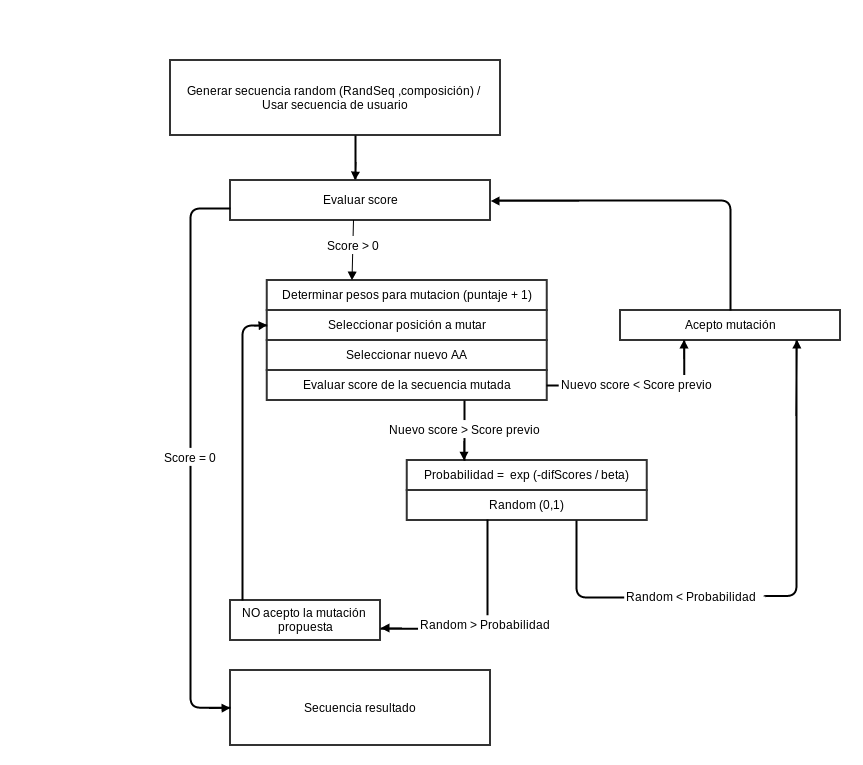
\includegraphics[width=\textwidth]{img/diagrama-algoritmo.png}
 \caption{Esquema general del método aplicado para obtener la secuencia final}
 \label{fig:esquema-algoritmo}
\end{figure}



\subsubsection{Método de mutación}
% POR QUE HACEMOS UNA MUTACION DE A 1 PASO, ES DECIR 1 SOLA MUTACION POR VEZ? 



% CAPITULO 3: POPIEDADES EVALUADAS / HERRAMIENTAS UTILIZADAS
\chapter{Análisis de las secuencias}
\label{tools}

En este capítulo se describen las evaluaciones que la herramienta permite realizar sobre las secuencias para detectar características deseadas y no deseadas dentro de la secuencia durante el proceso iterativo de diseño. 
Se explica en general cual es el objetivo de aplicar cada uno de los métodos y los fundamentos en los que se basan.
Se detalla como se integran los distintos recursos en el contexto de nuestra aplicación, representando sus resultados en el esquema de puntajes propio de nuestro método.

El conjunto de evaluaciones que se describen corresponde a esta primera versión de nuestra herramienta, por lo tanto no representa un conjunto exhaustivo ni definitivo, 
sino una primera etapa que deberá ser analizada y modificada de forma iterativa en función de los resultados obtenidos.
% hipotesis subyacente 

La definición del conjunto de evaluaciones utilizadas está directamente asociado a los fundamentos del método vistos en la sección \ref{fundamentos}.
Por un lado, se tiene en cuenta la hipótesis general sobre el espacio de secuencias buscadas, que nos permite asumir que este espacio es relativamente grande con respecto al conjunto total de posibles soluciones.
Por otro lado tenemos un conjunto de herramientas bioinformáticas que utilizan mecanismos y aproximaciones muy distintas y cuyos resultados pueden complementarse. 
Basándonos en estas propiedades, podemos pensar que la utilización de diferentes herramientas para la detección de caracteristica de interés, aún cuando algunos resultados de estas puedan solaparse entre si,
es una buena práctica al momento de definir el conjunto de herramientas utilizadas. 
% Como principio general para definir este conjunto, se tuvo en cuenta la hipótesis general sobre el espacio de secuencias buscadas, vista en la sección \ref{espacioSecuencial} . 
% De esta forma, dado que el espacio de soluciones buscadas se asume como considerablemente grande con respecto al espacio total de posibles secuencias, al hacer   
% una evaluacion sobrerestrictiva con respecto a las caracteristicas buscadas no se impediría alcanzar un resultado.

Por lo tanto, un aspecto que se repite es el solapamiento entre las características detectadas por las herramientas de evaluación, pensado con el fin de hacer mas exhaustiva la detección,
además de políticas considerablemente abarcativas en cuanto a los métodos, con el fin de asegurar una mayor cobertura de las propiedades buscadas.
Esta decisión permite dar mejores diseños finales, sin tener un aumento considerable en el tiempo de búsqueda.
Como complemento de esta política, parte del trabajo realizado durante el desarrollo de la herramienta consistió en implementar un código versátil que permita modificar fácilmente el conjunto de métodos de evaluación.
% La implementación está centrada en el esquema de mutaciones(visto en el capitulo previo) y es posible añadir herramientas de forma modularizada.
% Para esto, se debe agregar en la implementación una función independiente que tome como parámetro la secuencia correspondiente a evaluar y devuelva el puntaje asociado a cada posición. 
% Cualquier herramienta que pueda ser adaptada a este esquema podrá ser agregada a la implementación.



% Como complemento a esta idea de tener un amplio conjunto de propiedades/métodos a evaluar, se provee al usuario la posibilidad de seleccionar al momento de la ejecución 
% permite parametrizar la definición de las evaluaciones realizadas(\ref{evaluacion}). 
% Es decir, en cada ejecución, el usuario puede redefinir mediante parámentros el conjunto de evaluaciones realizadas seleccionando un subconjunto del total disponible, de acuerdo a sus propios objetivos específicos.


\section{Propiedades conformacionales} \label{propiedadesConformacionales}

Uno de los objetivos fundamentales de esta herramienta consiste en la restricción de elementos estructurales ordenados en la secuencia. 
Esto brinda al diseño resultante la flexibilidad requerida para la función de linker, adoptando una conformación intrínsecamente desordenada. 

En primer lugar vamos a utilizar la herramienta IUPred, descrita en la sección \ref{iupred}, para intentar detectar aquellas posiciones que puedan generar interacciones 
favorables en el contexto de la secuencia, indicando una tendencia a adoptar estructuras plegadas, caracteristicas de las proteínas globulares.


% %ESTO LO PASO DIRECTAMENTE A LA PARTE DE TMHMM 
% Sin embargo, la estabilización de estructuras tridimensionales puede deberse a otras interacciones con el contexto, que van mas allá de las interacciones intramoleculares.
% Las proteínas de membrana son módulos proteícos con propiedades secuenciales distintivas y que, a pesar de su diferencia con las proteínas globulares, 
% pueden adoptar una estructura tridimensional determinada, estabilizada por interacciones con el contexto hidrofóbico en el que normalmente se encuentran.
% Teniendo en cuenta este panorama más amplio, creemos conveniente agregar a la evaluación un predictor para identificar proteínas de membrana,
% principalmente de los segmentos transmembrana ya que son estos los que poseen propiedades particulares y, probablemente, no hayan sido detectados por el método anterior.
% Utilizamos la herramienta TMHMM(\ref{tmhmm}) para predecir su ocurrencia, profundizando nuestra capacidad de encontrar regiones propensas a formar estructuras ordenadas.

Por otro lado, utilizamos TMHMM (ver sección \ref{tmhmm}) para predecir la ocurrencia de segmentos transmembrana, 
los cuales presentan estructuras ordenadas y, por sus propiedadess particulares, probablemente no hayan sido detectados por el método anterior.




% *******************************************************
% ESTA PARTE QUE SIGUE LA BORRE PARA REDUCIR AL MAXIMO LA SECCION 3.1
% *************************************************************

% 
% % 
% % QUE METODOS EXISTEN
% Muchas de las propiedades vistas en la introducción sobre IDRs/IDPs(propiedades fisicoquimicas, composición, etc) pueden trasladarse fácilmente en herramientas de predicción.
% Además, se han desarrollado aproximaciones y métodos que hacen uso de distintos conceptos y conocimientos de IDPs estudiadas experimentalmente.
% Actualmente existen una gran cantidad de metodos diversos para predecir desorden estructural\cite{he2009predicting}, entre los que se incluyen
% % *** AGREGAR REFERENCIAS
% GlobBplot \cite{linding2003globplot}, PONDR, FoldIndex, DisEMBL, DISOPRED y DISOPRED2, IUPred, 
% FoldUnfold, RONN, DISpro, DisPSSMP y DisPSSMP2, Spritz , PrDOS , etc.
% 
% Para evitar detallar todos los métodos(ya que son muchos) usaremos la clasificación desarrollada en \cite{habchi2014introducing}, donde se analizan distintas 
% aproximaciones y se esboza una clasificación, concluyendo que el problema de la detección de IDPs  se puede atacar desde tres direcciones distintas:
% \begin{enumerate}
% 
% \item Los primeros predictores se basaron en propiedades de la composición y propiedades fisicoquímicas de la secuencia como la relación carga/hidrofobicidad. 
% Estas características(detalladas en la introducción ) se obtuvieron haciendo análisis estadísticos sobre conjuntos reducidos de IDPs/IDRs descubiertas inicialmente.
% % Como resultado de estos estudios se encontro que the ID proteins differ dramatically from the ordered proteins in their amino acid sequences. 
% 
% \item Distintas aproximaciones utilizan algoritmos de tipo \textit{machine-learning}. Estos y otros algoritmos de aprendizaje automático son ejecutado primero sobre datos de entrenamiento 
% (en este caso disintos conjuntos de secuencias que, se sabe, adquieren conformaciones no-plegadas) para intentar extraer un patrón propio del conjunto de datos.
% El algoritmo permite aplicar luego este patrón encontrado para predecir las mismas propiedades sobre un conjunto de datos nuevos. 
% La calidad del predictor resultante es muy variable ya que dependera del método aplicado, la representatividad del conjunto de entrenamiento usado y la complejidad del patrón a predecir.
% En particular, el número de IDPs determinadas experimentalmente es todavia pequeño y esto afecta considerablemente la calidad de los predictores desarrllados.
% Además se debe tener en cuenta que ciertas regiones pueden igualmente plegarse mediante procesos de binding and folding, por lo que la calidad de los datos de entrenamiento no está asegurada.
% 
% 
% \item Una gran cantidad de métodos siguen una aproximación común en el análisis de propiedades conformacionales que utiliza conocimientos sobre la propensión a formar interacciones entre cada par de AAs.
% La idea subyacente es que las IDPs no están plegadas porque no tienen la posibilidad de tener suficientes contactos entre sus residuos para superar la pérdida de entropía que ocurre durante el plegamiento.
% Es decir, en este tipo de conformaciones lo que se espera es que las interacciones posibles entre residuos no sean tan favorables.
% Esta hipótesis es aplicada de distinta forma para dar diversos métodos.
% A diferencia de los métodos mencionados en el punto anterior, los parámetros usados para hacer las evaluaciones son extraídos de datos conocidos sobre proteinas plegadas y/o IDPs ya que las 
% tendencias de interacción son las mismas para cualquier par de residuos en un mismo contexto.
% El conjunto de datos desde donde se extraen los conocimientos previos es mucho más númeroso(porque incluye bases de datos de estructuras ordenadas) y, por lo tanto, se espera que la predicción sea más acertada y menos sesgada.
% Se debe tener en cuenta que, como se vió en secciones previas, muchas IDRs pueden plegarse temporalmente en presencia de ciertos ligandos, por lo tanto cuando se extraen propiedades de bases de bases de datos de estructuras ordenadas 
% es posible que algunos datos tampoco sean totalmente válidos.   
% \end{enumerate}
% 
% 
% % It should be stressed that it is difficult and maybe impractical to establish the “best” predictor at the moment. 
% % Some predictors perform better on short disordered regions (i.e., DISOPRED2 and PreLink), 
% % while other predictors (IUPred for instance) perform well in predicting long disordered segments, and finally some predictors, such as PONDR, GlobPlot, and FoldIndex, 
% % have been trained on both short and long disorder and provide a balanced performance. 
% % Therefore, to avoid pitfalls, different predictors should be combined, as performed by metapredictors that seek a consensus of the scores of different predictors relying on different
% % principles (PONDR-FIT for instance).
% % To handle limitations inherent in prediction accuracy due to distinct flavors of disorder, however, different predictors are recently combined into metapredictors, such as metaPrDOS [9] or PONDR-FIT[10]. 
% % These combined predictors do show improved performance over their composite ones.
% 









% PEGAR EL TEMA DE AGREGACION DICIENDO COMO QUE ES OTRA FORMA DE INTERACCIONES QUE NO SON INTRAMOLECULARES PERO DAN UNA CONFORMACION TRIDIMENSIONAL NO-FLEXIBLE
% Otra forma de alcanzar una estructura tridimensional , como ya se describió, 
Los agregados proteicos son otro tipo de módulos que involucran la formación de una estructura tridimensional estable, en este caso mediante interacciones con otras unidades proteicas.
% Una estructura tridimensional rígida puede ser alcanzada por interacciones con otras proteínas, como se vió en la formación de agregados proteicos. 
Estas conformaciones agregadas pueden o no tener una estructura tridimensional ordenada pero, en todos los casos, limitan la flexibilidad requerida para una secuencia linker, generando, además,
módulos proteicos insolubles que afectan a todo el sistema biológico.
% Por lo tanto, a continuación nos centraremos en evitar la formación de agregados a partir del análisis secuencial.
Debido a estas implicancias altamente negativas se evaluará detalladamente la tendencia a formar agregados dentro de la secuencia que estamos diseñando.
 

Existe actualmente una gran variedad de métodos existentes para predecir agregación desestructurada y formación de fibras amiloides \cite{hamodrakas2011protein,redler2014computational,agrawal2011aggregation}.
Cada método hace sus propias hipótesis e implementa predictores independientes, los cuales varían desde análisis muy simples (por ej. análisis de la composición secuencial) a métodos específicos más complejos.
La capacidad para formar hojas-$\beta$ es una característica central de las evaluaciones ya que es un denominador común de la formación de agregados.

En primer lugar, en nuestra herramienta evaluaremos la tendencia a formar agregados utilizando TANGO (sección \ref{tango}). 
Para evaluar específicamente la formación de fibrillas amiloides utilizaremos Waltz (descrito en la sección \ref{waltz}), y PASTA (sección \ref{pasta}).
Por último, evaluamos la presencia de determinantes secuenciales que pueden indicar la formación de fibrillas amiloides, lo cual se describe en la sección \ref{determinantesSecuenciales}.



















% En el capítulo 1 nos centramos en la diferenciación entre proteínas plegadas y desordenadas, dado que esta clasificación era suficiente para introducir las conceptos de flexibilidad y desorden.
% A pesar que ya hemos mencionado las ideas de dominios/proteínas globulares, no detallamos la clasificación completa que contiene estos plegamientos, así es como, en general,
% las proteínas pueden clasificarse como globulares, de membrana, fibrosas o desordenadas, de acuerdo a las propiedades del plegamiento(o la falta de éste).


% *************************************************************
% FUNDAMENTOS DE LOS PREDICTORES DE SECUENCIAS TRANSMEMBRANA 
%    	PUEDE IR EN LA PARTE DE TMHMM   PERO LO SACO MOMENTANEAMENTE  ***  
% El conjunto de proteinas conocidas como de membrana posee una topología particular compuesta por segmentos que se encuentran insertados dentro del medio lipídico de la membrana y segmentos extra- e intra- celulares.
% Claramente, su conformación y composición está altamente marcada por estos dos tipos de segmentos ya que las interacciones que ocurren con el medio son totalmente distintas. 
% Estas propiedades hacen que se puedan diferenciar lo suficiente de otros tipos de proteínas plegadas como las globulares, que se mantienen normalmente solubles en el medio acuoso de la célula. 
% De hecho, los métodos mencionados para predecir conformaciones desordenadas están pensados en general como métodos para diferenciar entre éstas conformaciones desordenadas y las estructuras de proteínas globulares ya que,
% por ejemplo, cuando se evalúan las interacciones con el medio se asume que la proteína se encuentra en el medio acuoso, o cuando se utilizan datos de proteínas se filtran primero las proteínas de membrana(o los segmentos transmembrana) 
% para que sus propiedades secuenciales no provoquen una desviación de los datos. 
% Por lo tanto, para varios predictores no se espera que puedan diferenciar claramente el plegamiento que adquieren regiones transmembrana de una conformación con desorden intrínseco.


% La particularidad que presentan esta clase de proteínas es que las hélices transmembrana son considerablemente mas fáciles de predecir que las hélices en dominios globulares.
% La rason de esta mejora en la precisión se debe a que la mayoria de las helices transmembrana estan codificadas por una secuencia inusualmente larga de residuos hidrofóbicos, 
% que le permiten mantenerse estables en el nucleo de las membranas lipídicas.
% The hydrophobic signal is so strong that a straightforward approach of calculating a propensity scale for residues in
% transmembrane helices and applying a sliding window with a cutoff already performs quite well.


















% **********************************************************************
%    ESTE TEXTO QUE SIGUE LO BORRO COMPLETAMENTE, ANTES ESTABA PARA EXPLICAR la PERDIDAS DE FLEXIBILIDAD POR INTERACCIONES, FOLDING-AND-BINDING, CHAPERONAS, AGREGADOS..
%   LA PARTE DE CHAPERONAS Y MoREs  LA PASE A LA SECCION 3.2
% ***********************************************************************

% Hasta acá, intentamos asegurarnos que la secuencia no pueda adquirir una estructura ordenada de forma estable en su forma aislada.
% % Es decir, la perdidad de flexiblidad ocurria por interacciones intramoleculares.
% Sabemos, sin embargo, que la situación en el entorno celular es claramente diferente a esta condición ideal de aislamiento, 
% cualquier interacción con otros elementos que implique una reducción del ensamble conformacional, o lo que es lo mismo, 
% un aumento en las restricciones conformacionales, afectará directamente a la flexibilidad. 
% Para que la flexibilidad se mantenga en el contexto celular, intentaremos predecir perdidas de flexibilidad por interacciones con ligandos(otras proteinas iguales o distintas, DNA, membranas, etc).
% % y/u otras proteínas(iguales o distintas).
% 
% 
% % INTERACCIONES QUE ESTABILIZAN ESTRUCTURAS ORDENADAS --------- binding and folding
% En la sección \ref{proteinLandscape} se vió que, para las IDRs/IDPs, si bien su secuencia no tiene las caracteristicas necesarias para plegarse en una estructura ordenada, puede ocurrir que, ante la interacción con un ligando, 
% segmentos con estructuras ordenadas transitivas se estabilicen u otros segmentos experimenten un proceso de plegamiento, dando regiones con estructura ordenada estable como parte del complejo de interacción. 
% Si bien estos segmentos son muy importantes para la función de reconocimiento, en esta sección nos enfocamos en quitarlas por motivos estructurales, es decir, porque la adquisición de una estructura secundaria estable
% generaría una pérdida de flexibilidad en el linker.
% En nuestra evaluación utilizaremos ANCHOR\ref{anchor}, que busca identificar segmentos dentro de IDRs/IDPs que puedan adquirir una conformación rigida en estados de unión a ligandos.
% 
% % QUE OTRA HERRAMIENTAS EXISTEN!! !!! *****************
% % METODO DE DETECCION DE MoREs
% % Although the information content of short sites is very limited, due to their enrichment in hydrophobic residues, indirect techniques have
% % some success in delineating them. As mentioned, for example, the HCA plot 43 (see section 3.2) can indeed unveil such binding
% % sites. 25 The PONDR VL-XT, 23 ANCHOR (http://anchor.enzim.hu), 207 and DynaMine 208 disorder predictors are sensitive
% % to local tendency of ordering, and are thus informative in highlighting potential induced folding regions.
% 
% 
% 
% 
% 
% 
% 
% 

% 
% 
% % ACA CONECTO CON LA FORMACION DE AGREGADOS
% Existen chaperonas cuya función implica unirse a proteinas que no estén totalmente(correctamente) plegadas para evitar la agregación de estas. 
% El objetivo de esto es intervenir en situaciones ``anormales'', como por ejemplo estress térmico, donde la pérdida de la estructura nativa puede llevar a uniones entre distintas proteinas dando un agregado no funcional.
% Si bien uno de los objetivos de este trabajo es lograr una tendencia reducida a la agregación en la secuencia generada y 
% ciertas chaperonas podrían facilitar esto, la unión implica, como se menciono anteriormente, una pérdida de flexibilidad que es necesaria para la función de linker. 
% Por lo tanto, a continuación nos centraremos en evitar la formación de agregados a partir del análisis secuencial.
% % De esta forma buscamos evitar la agregacion mediante analisis sobre la secuencia que tienen este objetivo particular.
% 
% 
% 
% 
% % ***************************
% % ***********  AGREGACION !! 
% % POR QUE QUEREMOS/DEBEMOS PREVENIR LA FORMACION DE AGREGADOS
% % La formación de agregados es una forma especial de interacciones que involucra una gran cantidad de proteínas.  
% En primer lugar, la formación de agregados que involucren a las secuencias linker implicaría una clara reducción en la flexibilidad debido a la interacción con otras proteínas.
% Sin embargo, la interacción entre las secuencias linker y su consecuente pérdida de flexibilidad sería solo el principio del problema.
% Dadas las propiedades de los agregados, principalmente de la formación de fibras amiloides(estructura que se asume genérica de los polipeptidicos), 
% la formación de esta estructura abarcará a la secuencia completa de la proteína.
% En nuestro caso, la formación de fibrillas amiloides dentro de la secuencias linkers ``arrastraria'' a los dominios que únen a formar parte del agregado, interfiriendo directamente en la funcionalidad de estos. 
% La funcionalidad de cualquier dominio proteico se podria ver limitada si esta se encuentra formando algún tipo de agregado.
% En la sección \ref{agregados} se detallan los métodos usados para evaluar la tendencia a formar agregados sobe las secuencias.
% 























\subsection{IUPred: Análisis de tendencia al desorden} \label{iupred}

La herramienta IUPred \cite{dosztanyi2005pairwise} permite diferenciar secuencias con capacidad para formar plegamientos globulares de aquellas que no y, por lo tanto, están destinadas a permanecer en una conformación desordenada.
En nuestro método de evaluación, utilizamos esta herramienta para identificar aquellas posiciones que tienen una tendencia a formar conformaciones globulares en el contexto de la secuencia evaluada,
una propiedad que describimos como no deseada para secuencias linker.

% El método se basa en la estimación de la energía de interacción intramolecular, utilizando la secuencia
% Este modelo para describir la energia total en funcion de las interacciones puede representarse como:
% El primer paso en el desarrollo del método es el cálculo de una energía de interacción de a pares. Dada una estructura conformacional de una proteína, la :
% El método se basa en utilizar información de estructuras de proteínas globulares, las cuales. 
% Sabemos que podemos calcular la energía asociada a la estructura de una proteína mediante:




% ***********************
% DESCRIPCION DEL METODO
% ***********************
El primer paso del método es definir un modelo simple para calcular la energía total de una conformación nativa a partir de los contactos que se encuentran en esta:

% FORMULA 1
\begin{equation}\label{modelo1}
E = \sum_{ij=1}^{20} M_{ij}C_{ij}
\end{equation}

\noindent donde $M_{ij}$ es el potencial de interacción entre dos residuos de tipos $i,j$ (sólo depende del tipo de residuos), y $C_{ij}$ es el número de este par de residuos que se encuentran en contacto en la estructura.
% de contactos entre residuos de tipos $i,j$ encontrados en la estructura.

Sin embargo, el método IUPred busca poder evaluar la contribución energética de cada aminoácido usando, únicamente, la composición secuencial como parámetro. 
% Sin embargo, obviamente, se requiere conocer una estructura a partir de la cual extraer los pares que interaccionan y poder así evaluar el aporte energético de éstos.
% El centro de IUPred es poder evaluar la contribución energética promedio por AA en una secuencia usando como parámetro solamente su composición.
Esta evaluación tendrá la forma: 
% PONER FORMULA 2
\begin{equation}\label{modelo2}
\frac{E_{estimada}}{L} = \sum_{ij=1}^{20} n_{i}P_{ij}n_{j}
\end{equation}

\noindent donde $n_i$ y $n_j$ representan la frecuencia de residuos de tipo $i$ y $j$, respectivamente, en la secuencia.
P es la matriz de predicción de energia, que indica cómo la energía de un residuo de tipo $i$ depende de la existencia de residuos de tipo $j$ en el contexto.
% is the energy predictor matrix, which tells how the energy of amino acid i depends on the jth element of the amino acid composition vector.


% la idea es que la existencia de contactos(interacciones) favorables es resultado de las potenciales parejas de interacción en la secuencia.
% La idea es, entonces, obtener un potencial de interacción estadístico para cada par de AAs(Pij), el cual es totalmente independiente de la posicion que ocupan estos en la secuencia.
% Este valor representa la energia de interaccion entre cada ocurrencia del par ij en cualquier proteina.
% Es decir, para cada posible aminoacido i , saber como depende la contribucion energetica con respecto a la presencia de un aminoacido de tipo j en la secuencia.
% Conociendo este valor promedio, usando la ecuacion anterior(que solo depende de la composición) se podría obtener el valor de E por residuo (E/L).
% Lo que se requiere ahora es poder derivar la matriz P.

De esta forma, sin conocer la estructura de la proteína, basamos el cálculo de la energía en valores estadísticos (matriz P) que pueden ser extraídos de una base de datos de proteínas globulares.
Para esto, primero se desglosa la energía total de cada proteina en las contribuciones que hace cada aminoácido.
Esto puede hacerse reusando el modelo de la ecuación \ref{modelo1}, ya que conocemos las estructuras. 
La energía total por tipo de residuo se obtiene como:
% ecuacion de ek
\begin{equation}\label{ek1}
  e_i = \sum_{j=1}^{20} M_{ij}C_{ij}
\end{equation}
% Este valor depende de los contactos(interacciones) que hacen todos los aminoacidos de tipo i dentro de esa proteina. 
% En algunas estructuras, un par ij de aminoacidos estaran formando contactos , en otro no , en otro solo un par, etc...

Usando una aproximación similar a la de la ecuación \ref{modelo2}, esta energía por tipo de residuo se puede estimar mediante:
% la contribución de cada tipo de aminoacido a la energia de una proteina específica se puede estimar como:
% ecuacion ek estimado
\begin{equation}\label{ek2}
e_i(estimada) = N_i\sum_{j=1}^{20} P_{ij}n_{j}
\end{equation}
\noindent donde $N_i$ representa el número total de residuos de tipo $i$ en la secuencia ($L*n_i$).

% Utilizando las ecuaciones \ref{ek1} y \ref{ek2} tenemos la base para estimar cada valor $P_{ij}$ de la matriz a partir de los valores $M_{ij}$ y una base de datos de estructuras globulares conocidas.
Para esto estimar cada valor $P_{ij}$ de la matriz, se minimiza la diferencia entre los $e_i(evaluado)$ y los $e_i(calculado)$ para todas las estructuras de una base de datos de estructuras globulares.
% Dadas las propiedades de la ecuacion \ref{ek2}, la minimizacion se hace para cada fila de la matriz por separado.
La función a minimizar es, entonces: 
% funcion de Zi
\begin{equation}\label{z}
Z_i = \sum_{k} (e_i^k - N_i^k\sum_{j=1}^{20} P_{ij}n_{j}^k)^2   
\end{equation}
\noindent donde $k$ indica el índice de la estructura en la base de datos. 
% Es decir, se minimiza esta diferencia cuadrática para los valores de $e_i$ sobre todas las estructuras.


% Se tienen ahora los valores obtenidos de $P_{ij}$ los cuales son, luego, evaluados mediante la comparación de los cálculos de energía para un set de estructuras usando la ecuación \ref{modelo1} y la ecuación \ref{modelo2}, 
% obteniéndose una correlación que indica, de acuerdo a los análisis estadísticos aplicados, un nivel razonable de concordancia entre ambos cálculos.

Tenemos ahora un modelo completo que nos permite estimar la energía miníma de la estructura asociada a una secuencia, sin asumir ninguna conformación (\ref{modelo2}).
Este modelo primero se prueba sobre dos conjuntos de proteinas globulares e IDPs obteniéndose que la energia estimada para el conjunto de IDPs son menos favorables que las correspondientes al set de proteínas globulares,
lo que esta de acuerdo con la hipotesis que indica que las proteinas globulares tienen secuencias especificas con potencial para formar un gran numero de interacciones favorables, mientras que las IDPs no.
Utilizando esta separación significativa, lo que resta es transformar esta aproximación en un método para predecir el desorden a partir de la secuencia, 
para lo cual se transforma el valor de energía en un valor de probabilidad (\textit{score} resultante, $s_k$).



% *********************************************
% % SACO ESTA ULTIMA PARTE  EXPLICA COMO SE ADAPTA P PARA TENER EN CUENTA SOLO EL CONTEXTO CERCANO DE CADA POSICION
% *********************************************
% Sin embargo, el modelo se debe adaptar ya que es mas realista si se consideran solo la composición de la secuencia mas próxima a la posición que se está analizando, de manera que se puedan analizar por regiones desordenadas/ordenadas.
% Para esto se recalculan los valores de la matriz $P_{ij}$ pero cada posición se trata de forma separada teniendo en cuenta, solamente, la secuencia del contexto
% (sólo se tienen en cuenta posibles interacciones con residuos a distancias entre 2 y 100 posiciones alrededor).

% % SACO ESTA ULTIMA ECUACION, ME PARECE QUE QUEDA BASTANTE CLARO EN EL TEXTO
% La energía de a pares asociada a cada posición $k$ de una secuencia se calcula ahora según la ecuación \ref{modelofinal}.
% 
% \begin{equation}\label{modelofinal}
% E_i^k = \sum_{j=1}^{20} P_{ij}f_{j}^k(w_o) 
% \end{equation}
% 
% donde $f_{j}^k(w_o)$ es la fracción de residuos de tipo $j$ en el entorno de la posición $k$

% % ESTO LO PUSE ANTES, PORQUE SAQUE LA ULTIMA ECUACION
% El resultado final de la predicción consiste en la transformación del valor de energía en un valor de probabilidad(\textit{score} resultante, $s_k$).








% *************************
% UTILIZACION DEL METODO 
% ***********************
La herramienta para el cálculo del score a partir de una secuencia está disponible a través de un servidor web \cite{iupredWeb,dosztanyi2005iupred} o descargando la implementación y ejecutándola localmente \cite{iupredDownload}.   
En nuestro caso utilizaremos la segunda opción. 
Tal como se menciona en la información del servidor \cite{dosztanyi2005iupred}, los residuos que tengan un valor asociado de \textit{score} mayor a 0.5 pueden ser tomados como desordenados.
Por lo tanto, en nuestro método, los residuos que posean un \textit{score} resultante menor a 0.5 tendrán un valor de 1 en el puntaje asociado a la posición.
Por ejemplo, la evaluación de la secuencia \texttt{VLKQTKGVGASGSFR} con IUPred devuelve los valores de score que se ven en la figura \ref{iupredResults}
% PONER RESULTADOS DE IUPred EN GRAFICO O TABLA

\begin{figure}[h!]
% {\linewidth}
\centering
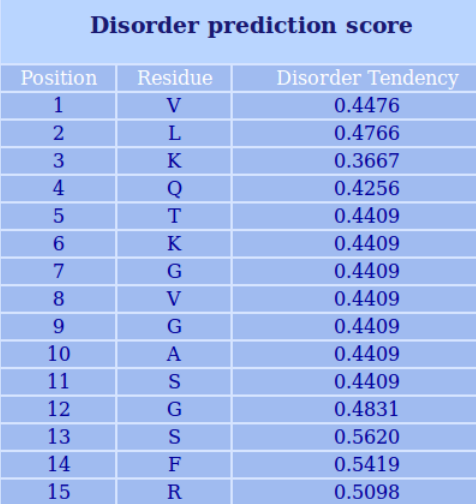
\includegraphics[width=0.5\textwidth]{img/iupredTabla.png} 
\caption{}
\label{iupredResults}
\end{figure}

Utilizando nuestro esquema de evaluación, estos valores resultan en los siguientes puntajes:

\vspace{0.5cm}
\begin{tabular}{lllllllllllllllll} 
\hline
Secuencia & \textbf{V} & \textbf{L} & \textbf{K} & \textbf{Q} & \textbf{T} & \textbf{K} & \textbf{G} & \textbf{V} & \textbf{G} & \textbf{A} & \textbf{S} & \textbf{G} & \textbf{S} & \textbf{F} & \textbf{R} \\ \hline
Evaluación con IUPred & 1 & 1 & 1 & 1 & 1 & 1 & 1 & 1 & 1 & 1 & 1 & 1 & 0 & 0 & 0\\ \hline
\end{tabular}







% 
% 
% 
% 
% 
% % RESUMEN SACADO DEL REVIEW
% % 
% % Dosztanyi et al. suggested that a large number of interresidue interactions is responsible for structure stabilization of proteins [50, 51]. In contrast, IDPs don’t have sufficient numbers of stabilizing inter-residue interac-
% % tions. Based on this reasoning, an IUPred algorithm estimating the inter-residue interactions was designed. First, the interaction energy between each pair of amino acids
% % based on their C β positions was estimated. This was done by calculating the potential mutual contact energies for
% % all amino acid pairs in a dataset of globular proteins with known structure. This is a fairly standard approach in
% % computational biology, and in this work Dosztanyi et al. compared several such mutual contact energies estimated
% % previously by other researchers, with the set developed by Thomas and Dill, found to be the best in this particu-
% % lar application [92]. The various pairwise energies were assembled into a 20x20 energy matrix, which was used
% % in the next step, the estimation of the mutual interaction energies for any given protein. The prediction utilizes
% % this energy prediction matrix and the amino acid compositions put into a quadratic expression. These statistical values represent the ability to form stabilization contacts
% % between amino acids in polypeptide chains. The potential mutual interactions were estimated using amino acid
% % compositions, not three-dimensional structures. These composition-based energies were compared with three-
% % dimensional structure-based energies of the proteins for which the actual side chain interactions are known. The
% % composition-based potential mutual interaction energies and the structure-based energies were found to be highly
% % correlated, thus the former can be used to estimate the latter even when the structures are not known. To use
% % this approach to predict structure or disorder, composition-based calculations for a set of proteins that fold
% % into three-dimensional structures were compared with composition-based calculations for a set of disordered
% % proteins. The estimated potential interaction energies for the structured proteins were much greater than the same
% % energies for the unstructured proteins, and from these results the energy boundary between ordered and disor-
% % dered proteins as a function of length was determined. This boundary allows the recognition of intrinsic disor-
% % der. In brief, if a sequence contains too few hydrophobic residues, then the composition-based potential mutual in-
% % teraction energy will necessarily be too small and thereby indicate the lack of potential for folding
% 



% Partiendo del concepto general que la conformación nativa está determinada por la estructura primaria de la proteína, y que esta conformación se corresponde con el mínimo global del
% espacio conformacional, es posible parametrizar un modelo que permita predecir este mínimo de energía sin asumir ninguna conformación estructural. (Ref. 2)
% Esta aproximación es posible ya que la contribución energética de un residuo depende, no solo del tipo de aminoácido, sino también de los potenciales parejas de interacción en la secuencia. 
% El aporte de un residuo será más favorable si la secuencia en la que se encuentra contiene más residuos que pueden formar interacciones favorables con este. 
% La forma de plantear este modelo es mediante una expresión cuadrática sobre la composición de aminoácidos de la secuencia:
% Los valores de n representan las frecuencias de aminoácidos i y j en la secuencia.
% El valor de P es el parámetro a estimar, el cual se deriva a partir del modelo mencionado previamente, que evalúa la energía a partir de las interacciones que ocurren en la estructura. 
% El ajuste se realiza minimizando la diferencia entre ambas ecuaciones.
% De esta forma, mediante un ajuste de mínimos cuadrados se puede parametrizar el modelo a partir de datos de estructuras pertenecientes a proteínas globulares.
% Dado que las proteínas globulares forman un gran número de interacciones entre los residuos (lo que les provee la energía estabilizante para superar la pérdida de entropía), 
% y las proteínas IU/desordenadas tienen secuencias especiales que no poseen esta capacidad de formación de interacciones, la estimación del potencial de interacción permite diferenciar entre 
% regiones de proteínas ordenadas y desordenadas. Esto transforma el modelo de predicción en un eficiente método para diferenciar secciones desordenadas de secciones con estructura definida.
% 
% Como se mencionó previamente, la parametrización de este modelo se realiza a partir de estructuras contenidas en una base de datos de proteínas globulares, 
% por lo que son datos suficientes para realizar una buena parametrización, además de ser consistentes y curadas. Esto diferencia el método de otros, que se basan en adaptar 
% un modelo a datos de estructuras correspondientes a proteínas intrínsecamente desordenadas, agrupados en bases de datos chicas, con datos obtenidos usando diversas técnicas 
% y con distintos significados del término desordenado.
%   

%   

  
  
  
  

  
  
  
  
  
\subsection{TMHMM: Secuencias transmembrana} \label{tmhmm}

% QUE QUEREMOS DETECTAR
% La estabilización de estructuras tridimensionales puede deberse a interacciones con el contexto, que van mas allá de las interacciones intramoleculares.
Las proteínas de membrana son módulos proteícos con propiedades secuenciales distintivas y que, a pesar de su diferencia con las proteínas globulares, 
pueden adoptar una estructura tridimensional determinada, estabilizada por interacciones con el contexto hidrofóbico en el que normalmente se encuentran.
Teniendo en cuenta este panorama más amplio, utilizamos el predictor TMHMM \cite{krogh2001predicting} para identificar proteínas de membrana,
principalmente de los segmentos transmembrana ya que son estos los que poseen propiedades particulares y, probablemente, no hayan sido detectados por otros métodos de nuestra evaluación.

% EL MÉTODO
TMHMM es un método para detección de segmentos transmembrana que utiliza una aproximación mediante modelos ocultos de Markov (Hidden Markov Models, o HMM).
Un HMM representa un modelo de Markov con estados no visibles. Es decir, el sistema es descrito por un modelo estocástico representado por estados y transiciones entre estos, las cuales están determinadas únicamente por el estado actual.

Describiendo el modelo de Markov que represente a la arquitectura de una proteína transmembrana se puede conocer si una secuencia desconocida pertenece a esta clase, evaluando si se adapta a este modelo.
Para poder describir una proteína mediante un HMM se debe definir un conjunto de estados, cada uno correspondiente a una región o sitio específico de la proteína que se está modelando.
Cada estado tendrá un valor de probabilidad asociado a cada uno de los 20 aminoácidos posibles. Además, se deben definir las transiciones posibles(y las probabilidades asociadas) entre los estados según la arquitecura que se está describiendo, por ejemplo si a partir 
de un estado pueden ocurrir nuevas instancias de este o si debe pasarse a un nuevo estado determinado.
La distribución de probabilidades de los aminoácidos en cada estado y la probabilidad de transición se derivan a partir de frecuencias observadas en un conjunto de proteínas conocidas que se adaptan al modelo

El modelo utilizado para describir la arquitectura de las proteínas en el método TMHMM (proteínas transmembrana) es cíclico y está compuesto por 7 estados distintos que representan: el núcleo de la hélice transmembrana, los dos extremos de ésta, 
el loop que se encuentra en el lado citoplasmático, dos loops en el lado no-citoplasmático, y un dominio globular en el medio de estos. En la figura \ref{tmhmmModel} se ve la descripción gráfica de este.
En \cite{sonnhammer1998hidden} se describe como se procede al entrenamiento del HMM para poder obtener todos los parámetros asociados.


\begin{figure}[h!,centered]
\centering
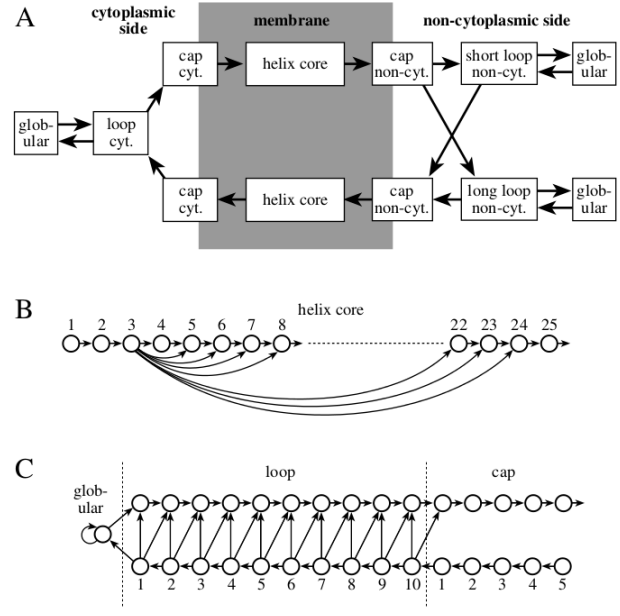
\includegraphics[width=0.7\textwidth]{img/tmhmmModel.png} 
\caption{\textbf{A:} esquema general de la arquitectura asociada al modelo. En \textbf{B} y \textbf{C} se muestran en detalle algunos de los estados y cómo las
transiciones entre estos permite definir los limites en las longitudes de las distintas regiones y sus propiedades. Figura extraida de \cite{sonnhammer1998hidden}}
\label{tmhmmModel}
\end{figure}


Para evaluar secuencias se utiliza el algoritmo de Viterbi, el cual permite calcular cual es el camino más probable del modelo que adopta la secuencia a evaluar. Es decir, cual es la secuencia mas probable de estados del HMM 
(entre todas las posibles), que produce la secuencia de estados observados (aminoácidos de la secuencia).
El resultado de la ejecución muestra cómo los residuos de la secuencia se ajustan a los diferentes estados del modelo de acuerdo a este recorrido más probable, clasificándolos según pertenezcan a regiones intracelulares, hélices transmembrana, 
o regiones extracelulares. 
% MODO DE UTILIZACION
Este método puede ser ejecutado como servicio web o descargado como paquete de software en \cite{tmhmmServer}.
En nuestro caso realizamos la ejecución de manera local.

Nuestro interés está en detectar las regiones que forman los segmentos transmembrana, por lo tanto, el puntaje resultante será igual a 1 para aquellas posiciones que pertenezcan a estos segmentos y 0 para el resto. 
Por ejemplo, la ejecución de TMHMM a partir de la secuencia \texttt{NFVLIGSFVAFFVITYFLE} devuelve los siguientes resultados: 

% \noindent
\texttt{inside         1-1}\\
\indent \texttt{TMhelix   2-18}\\
\indent \texttt{outside	    19-19}\\

Por lo tanto, el puntaje resultante de la evaluación es:

\vspace{0.5cm}
\noindent
\begin{tabular}{lllllllllllllllllllll} 
\hline 
Secuencia & \textbf{N} & \textbf{F} & \textbf{V} & \textbf{L} & \textbf{I} & \textbf{G} & \textbf{S} & \textbf{F} & \textbf{V} & \textbf{A} & \textbf{F} & \textbf{F} & \textbf{V} & \textbf{I} & \textbf{T} & \textbf{Y} & \textbf{F} & \textbf{L} & \textbf{E}  \\ \hline
Puntaje TMHMM & 0 & 1 & 1 & 1 & 1 & 1 & 1 & 1 & 1 & 1 & 1 & 1 & 1 & 1 & 1 & 1 & 1 & 1 & 0\\ \hline
\end{tabular}



 
 
 
 



% ******************************************************************************** 
% ******************************************************************************** 
% 	FORMACION DE AGREGADOS, BORRO COMPLETAMENTE LA INTRO A  ESTA SECCIÓN ...
%	QUEDA TODO DESCRITO EN CADA METODO INDIVIDUAL USADO (TANGO, PASTA,.. )
% ******************************************************************************** 
% ******************************************************************************** 
% 
% 


% 
% \subsection{Formación de agregados}
% \label{agregados}
% 
% 
% % En el capítulo 1 vimos las propiedades más importantes de los agregados formados por proteínas.
% 
% 
% La formación de agregados amorfos y de fibrillas amiloides son procesos diferentes, sin embargo comparten ciertas características similares ya que ambos están asociados con el enriquecimiento de estructuras de hojas-$\beta$ 
% en la forma agregada, por lo que en gran medida pueden analizarse de forma conjunta.
% 
% Como se vió, la estructura de las fibrillas amiloides es altamente estructurada y por lo tanto las preferencias de aminoácidos serán mucho más específicas en relación a la posición comparado con la formación de agregados amorfos.
% La formación de estos agregados amorfos es mucho menos dependiente de los residuos en cada posición y, por lo tanto, su tendencia puede predecirse si se evaluan los parámetros biofísicos generales sobre la comppsición, sin necesidad de 
% evaluar propiedades específicas de secuencia.
% % y, en principio, cualquier secuencia que adopte una conformación extendida, no tenga grupos  y sea suficientemente hidrofóbica 
% % puede agregarse para dar esta conformación
% % Amorphous $\beta$-sheet aggregation, however, is less position-dependent and can, in principle, be achieved by any sequence that can adopt an extended conformation, 
% % is sufficiently hydrophobic and has no unsatisfied hydrogens or electostatic groups. 
% % POR QUE NO USAMOS UN PREDICTOR ESPECIFICO??
% 
% 
% % METODS DISPONIBLES PARA HACER LA DETECCION
% En \cite{hamodrakas2011protein,redler2014computational,agrawal2011aggregation} se describen y evaluan una gran cantidad de software/metodos existentes para predecir agregacion desestructurada y formación de fibras amiloides, 
% Cada método hace sus propias hipótesis e implementa predictores independientes, los cuales varían desde análisis muy simples (por ej. análisis de la composición secuencial) a métodos específicos más complejos.
% La capacidad para formar hojas-$beta$ es una característica central de las evaluaciones ya que es un denominador común de la formación de agregados.
% 
% 
% 
% 
% En primer lugar evaluaremos la tendencia a formar agregados utilizando TANGO(ver sección \ref{tango}). 
% El método utilizado por TANGO, centrado en calcular la función de partición para distintos estados conformacionales, nos permite también evaluar la tendencia a adoptar estructuras nativas como hélices-$\alpha$ y $\beta$-turn,
% además de la tendencia a la formación de agregados. 
% % Este método se basa en el uso de principios fisicoquímicos que gobiernan la formacion de hojas-$\beta$
% % extended by the assumption that the core regions of an aggregate are fully buried
% % , de manera que el método no es específico para la formación de agregados amorfos o amiloides.
% % Like all algorithms that use averaged physicochemical properties to detect aggregation hot spots, TANGO is not specific for amyloid formation or amorphous beta-aggregation. 
% 
% 
% 
% % En cuanto a los agregados amiloides específicamente, 
% En la introduccion se plantearon algunas propiedades fisicoquimicas simples con respecto a la composición de secuencias con tendencia a formar estas estructuras agregados amiloides específicamente.
% En particular, las características mas importantes son la alta hidrofobicidad y baja carga neta, además de tendencia intrinseca a adoptar conformaciones de hoja-$\beta$ en su estructura primaria.
% Se cree que las regiones propensas a formar agregados(APRs como se vió previamente) son segmentos con estas características que normalmente se encuentran ocultos en el núcleo hidrofóbico de la estructura plegada pero
% bajo condiciones de reestructuración del plegamiento o cuando se adoptan estados \textit{misfolded}, estos segmentos pueden quedar expuestos al solvente e iniciar la formación de agregados.
% 
% % \cite: The triple power of D-3: Protein intrinsic disorder in degenerative diseases
% Estos conocimientos forman la base para el desarrollo de una gran variedad de aproximaciones bioinformáticas para predecir tendencias a formar agregados a partir de la secuencia primaria.
% Se debe tener en cuenta, a la hora de analizar los resultados obtenidos con esto métodos, que la existencia de APRs en la secuencia es una condición necesaria pero no suficiente para la formación de agregados
% 
% 
% Algunos métodos intentan distinguir los agregados amorfos de la formación de fibrillas amiloides. 
% Sin embargo, dado que la cantidad de secuencias que generan estructuras amiloides y se han validado experimentalmente es relativamente baja, los algoritmos basados puramente en secuencia no poseen 
% suficiente información como para distinguir los distintos tipos de agregados.
% % They generally also have rather poor predictive capabilities toward amyloid sequences from yeast prions and functional amyloids. 
% Por otro lado, los métodos que se basan en conceptos estructurales obtenidos por homología pueden, en principio, proveer predicciones más específicas aunque también están limitados por la cantidad de estructuras determinadas disponibles.
% 
% Para evaluar específicamente la formación de fibrillas amiloides utilizaremos, en primer lugar, Waltz (descrito en la sección \ref{waltz}),
% el cual combina información secuencial, parámetros fisicoquímicos y aspectos estructurales que, como se dijo, pueden no funcionar muy bien de forma aislada pero permitir una predicción eficiente si se combinan.
% 
% 
% % PASTA
% PASTA es otra de las herramienta que utilizamos para evaluar la tendencia a formación de agregados amiloides. 
% PASTA obtiene potenciales estadisticos para la formación de estructuras de hojas-plegadas-$\beta$ a partir de proteinas globulares y los utiliza para
% predecir cuales son los segmentos de una secuencia que le proveen a la proteína la capacidad de estabilizar la estructura supramolecular cross-$\beta$ característica de las fibrillas amiloides.
% % predicts which interacting portions of a given protein are stabilizing the cross-beta structure by using an energy function. 
% % r las energias asociadas a distintos emparejamientos entre secuencias formando una estructura tipo fibrilla amiloide. 
% 
% Por último, en el capítulo 1 se dejó planteada la idea sobre la existencia de subsecuencias que podrían promover y guiar la agregación para dar estructuras amiloides.
% En el trabajo realizado en \cite{de2004sequence} se analiza esta idea y en \ref{determinantesSecuenciales} explicamos los resultados obtenidos y como los utilizamos para la detección 
% de la tendencia a formar este tipo de agregados dentro de nuestro método.
% 




























\subsection{Tango}\label{tango}


TANGO \cite{fernandez2004prediction} es un método utilizado principalmente para predecir regiones de agregación $\beta$, desarrollado a partir de un modelo de mecánica estadística que define 
un espacio de fases incluyendo, además de estos agregados, conformaciones de $\beta$-turn, hélices-$\alpha$ y hebras-$\beta$.
En nuestro sistema de evaluación, deseamos evitar tanto las conformaciones agregadas como cualquier otra estructura ordenada, por lo tanto utilizaremos TANGO para detectar las posiciones que tienen tendencia a encontrarse formando
alguna de estas conformaciones.
% el estado nativo de la proteína??.

De acuerdo con el modelo definido por TANGO, cada segmento de un péptido/proteína puede encontrarse en alguno de estos estados de acuerdo a una distribución de Boltzmann. 
Es decir, la frecuencia con la que el segmento se encuentra en alguno de los posibles estados, es relativa a la energía asociada a este, la cual se deriva de consideraciones empíricas y estadísticas. 
% Para cada conformación posible se realizan consideraciones y evaluaciones energéticas con respecto al estado desplegado.
De esta forma, el método consiste de un algoritmo que simplemente calcula la función de partición y en base a eso predice las regiones con tendencia a agregación $\beta$

Puntualmente, para el cálculo de la energía asociada a la conformación de hélice-$\alpha$, se tienen en cuenta los parámetros definidos previamente en el desarrollo del método AGADIR \cite{lacroix1998elucidating}.
Para el cálculo de la energía asociada a las conformaciones $\beta$ se tiene en cuenta la energía de interacción entre las cadenas laterales.
Esta energía se deriva, a partir de una base de datos de estructuras, calculando la relación entre frecuencias observadas y esperadas para cada par de aminoácidos que se encuentra en este tipo de conformación.
% (identificados en conformación $\beta$ de acuerdo a sus ángulos phi y psi).
% Para evaluar esta energía entre cualquier par de aminoácidos en conformación de $\beta$-strands, se calcula un potencial estadístico a partir de la relación 
% entre la frecuencia observada y la frecuencia esperada para los pares encontrados dentro de una base de datos(identificados en conformación $\beta$ de acuerdo a sus ángulos phi y psi).
Asumiendo que la base de datos representa un sistema termodinámico en equilibrio, la frecuencias se relacionan con la energía de interacción de acuerdo a la siguiente ecuación:

\begin{equation}
\large
 \Delta G_{interacc-cadenas}=-RTln(\frac{f_{observada}}{f_{esperada}})
\end{equation}

% ESTA ACLARACION NO SE SI ES NECESARIA, CONFIRMAR SI ESTA ESCRITA CORRECTAMENTE
% \noindent donde $\Delta G_{interacc-cadenas}$ representa la diferencia en energía libre entre la conformación desplegada del polipéptido y la interacción formando la conformación definida.

Para el caso en que la conformación sea de $\beta$-turn, dado que los residuos no están fijos sino que pueden adoptar diferentes conformaciones, se agrega una penalización por el aumento de entropía.
% Este valor empírico es de 0.3 Kcal/mol
Por otro lado, en el caso de agregados $\beta$ se asume que los residuos que adoptan esta conformación se encuentran completamente insertos en el núcleo y pagan el costo energético correspondiente. 
En este caso se calculan los diferentes parámetros energéticos, de hidrofobicidad, de solvatación, las interacciones electrostáticas y las interacciones por formación de puentes de hidrógeno.

A partir de las energías definidas para estas cuatro conformaciones, se calcula la función de partición resultante que permite definir las tendencias de cada residuo a poblar los distintos estados conformacionales evaluados.
La salida que muestra TANGO se compone de un archivo con las siguientes columnas:
Número de posición, residuo en esa posición, porcentaje en conformación hebra-$\beta$, porcentaje en conformación $\beta$-turn, porcentaje en conformación hélice-$\alpha$, porcentaje de agregados $\beta$ y
porcentaje en agregación de hélices-$\alpha$.
Esta última columna no forma parte del modelo inicial que describimos y se calcula aparte, no representando un resultado confiable.
% , por lo tanto la suma total puede dar mayor a 1.

El método puede ser utilizado a través del servidor web en \cite{tangoWeb}. En nuestro caso solicitamos a los creadores especialmente una versión ejecutable para poder usarla de manera local.
Una vez ejecutados y obtenidos los resultados para una secuencia, es necesario definir un valor de \textit{threshold} que determine la significancia de la tendencia obtenida.
En \cite{fernandez2004prediction} se definen dos intervalos de confianza para la predicción de regiones de agregación: segmentos con residuos que posean más de 5\% de tendencia agregación $\beta$ (resultando en una alta certeza de predicción),
y segmentos con residuos entre 0.2\% y 5\%. En nuestro caso utilizamos 1\% como valor de \textit{threshold} en esta primera implementación de la herramienta.
% Si bien el objetivo principal de TANGO, y de la aplicación de este en nuestra herramienta, es buscar segmentos con potencial de agregación, estamos interesados en eliminar cualquier región estructurada y, dado que TANGO incorpora como parte
% de la función de partición a distintos estados conformacionales nativos, el puntaje reflejará también todas estas tendencias en la secuencia. 

Dado que TANGO fue desarrollado con el objetivo de evaluar tendencias a formar agregados, no se evaluaron las predicciones asociadas a otros estados conformacionales. 
Para utilizar estas evaluaciones en nuestra implementación utilizaremos el mismo valor de \textit{threshold} que se obtuvo para la predicción de agregación $\beta$. 
Por lo tanto, el puntaje será igual a 1 cuando el residuo tenga una tendencia superior al valor de \textit{threshold} para la formación de agregados, hélices-$\alpha$, hebras-$\beta$ o $\beta$-turns, 
y un puntaje igual a 0 en caso contrario.
Por ejemplo, si evaluamos usando TANGO la secuencia \texttt{AMAPVLYLQDKSS}, obtenemos la siguiente tabla de valores:

\vspace{0.3cm}
\begin{center}
\begin{tabular}{ccccccc}
Pos & Residuo & Beta & Turn & 	Hélice & Beta Aggregation & Helical Aggregation\\
01 &          A & 0.2 & 0.0 &  0.000  & 0.000 &  0.000\\
02 &          M  &     0.2 &    0.0 &  0.000 &  0.000 &  0.000\\
03 &          A &      0.2  &      0.0 &  0.000 &  0.000  & 0.000\\
04  &         P &      0.0   &     0.0 &  0.000 &  0.544  & 0.544\\
05  &         V &      1.6   &     0.0 &  0.000 &  10.620 & 10.620\\
06   &        L &      2.3   &     0.0 &  0.000 &  10.620 & 10.620\\
07      &     Y &      3.1   &     0.0 &  0.000 &  10.620 & 10.620\\
08        &   L &      1.7   &     0.2 &  0.000 &  10.620 & 10.620\\
09         &  Q &      1.0   &     0.2 &  0.000 &  10.203 & 10.203\\
10   &        D &      0.3    &    1.8 &  0.000 &  0.000 &  0.000\\
11  &         K &      0.3   &     1.8 &  0.000 &  0.000 &  0.000\\
12  &         S &      0.2   &     1.6 &  0.000 &  0.000 &  0.000\\
13  &         S  &     0.2  &      1.6 &  0.000 &  0.000 &  0.000\\
\end{tabular}
\end{center}

\vspace{0.5cm}
El segmento en las posiciones 5-9 supera el porcentaje de agregación que utilizamos como threshold, mientras que el segmento 10-13 supera este valor en la tendencia a encontrarse en conformaciones de $\beta$-turn.
Por lo tanto, el puntaje resultante de la evaluación es:

\vspace{0.5cm}
% \noindent
\begin{center}
\begin{tabular}{llllllllllllll} 
\hline      		
Secuencia & \textbf{A} & \textbf{M} & \textbf{A} & \textbf{P} & \textbf{V} & \textbf{L} & \textbf{Y} & \textbf{L} & \textbf{Q} & \textbf{D} & \textbf{K} & \textbf{S} & \textbf{S} \\ \hline
Evaluación con TANGO & 0 & 0 & 0 & 0 & 1 & 1 & 1 & 1 & 1 & 1 & 1 & 1 & 1 \\ \hline
\end{tabular}
\end{center}





% 
% ****la inclusion del estado plegado dentro de la funcion de particion tiene como objetivo ayudar a predecir efectos de agregacion debido a mutaciones puntuales en proteinas que naturalmente adquiren un estado plegado. 
% La inclusion de este estado permite ver la competencia entre este estado natural de plegado y otros estados estructurales incluidos en la particion. 
% De esta forma se puede predecir la tendencia a la agregacion del estado desnaturalizado y tambien las mutaciones que aumentan la tendencia a la agregacion de la proteina desestabilizando el estado plegado.








\subsection{PASTA}\label{pasta}


PASTA \cite{trovato2006insight} es una herramienta que permite, principalmente, predecir las regiones de un polipéptido que pueden estabilizar la estructura de las fibrillas amiloides.
Para esto, realiza un cálculo de las energías de interacción entre los distintos segmentos, asumiendo que el mecanismo de las interaccion entre aminoácidos que lleva a la formación 
de láminas-$\beta$ en proteínas globulares es el mismo que lleva a la formación de apilamientos de hebras-$\beta$ en estructuras cross-$\beta$.
% (estructura asociada a fibras amiloides).

% En primer lugar, Pasta deriva una funcion energetica a partir de un conjunto de datos de estructuras globulares (potenciales estadisticos).
La evaluación de la energía de interacción se realiza a partir de un potencial estadístico derivado de una base de datos de proteínas globulares.
% (selección de proteínas no-redundantes y con estructuras resuletas con alta definición)
Para esto, se dividen las instancias encontradas de cada par $a$-$b$ de residuos en 4 categorias, según estén interaccionando formando una hoja plegada-$\beta$ en forma paralela ($n_{ab}^p$) o antiparalela ($n_{ab}^p$), 
o si no están participando de una estructura $\beta$ y sus carbonos-$\alpha$ están a menos de $6.5$\AA ($n_{ab}^c$ contactos genéricos), o a más de $6.5$\AA ($n_{ab}^d$ , pares desordenados sin contacto). 
A partir de las frecuencias obtenidas se pueden derivar valores de energía asociados a las interacciones de a pares para los distintos estados, asumiendo que la base de datos analizada es un sistema en equilibrio termodinámico 
a temperatura constante para todas las proteínas.
De esta forma, la probabilidad de cada par $a$-$b$ de encontrarse en un estado $x$ se relaciona con el valor de la energía mediante el factor de Boltzman $p_{ab}(x)= e^{-E_{ab}^x}$. 

Si podemos obtener una aproximación para $p_{ab}(x)$ se puede despejar el valor del potencial de interacción estadístico asociado ($E_{ab}^x$) para cada estado $x$,
el cual corresponde a la diferencia en energía entre el estado $x$ y el estado que se toma como referencia.
Definiendo la probabilidad $p_{ab}(x)$ como la relación entre la frecuencia de interacciones observada para cada par y la esperada en el estado de referencia, 
y aproximando esta última como la frecuencia observada para todos los pares, se obtiene:
% Utilizando los valores definidos previamente, se despeja el 
% Despejando el valor de $E_{ab}^x$ para cada estado $x$, el cual corresponde a la diferencia en energía entre el estado $x$ y el estado que se toma como referencia, se obtiene:
% El método asume que la forma soluble(estado de referencia) es nativamente desestructurada, por lo que hay que tener cuidado cuando se lo usa para predecir proteinas que nativamente adquieren una estructura globular.
% El valor de energía resultante para cada estado $x$ queda definido por:

\begin{equation}
{E_{ab}^x = -log\left(\dfrac{\dfrac{n_{ab}^x}{n_{ab}}} {\dfrac{\sum\limits_{ab} n_{ab}^x}{\sum\limits_{ab} n_{ab}}}\right)}
\end{equation}


% Para derivar este valor, lo que hace es ver cual es 
% la probabilidad de encontrar cierto par de residuos enfrentados en hebras vecinas dentro de una lámina-$\beta$. 
% Se extraen valores de potencial según estén interaccionando en sentido paralelo o antiparalelo.
% El valor de este potencial estadistico para cada clase(paralela,antiparalela, etc) se calcula según la relación entre la frecuencia observada y la frecuencia esperada:
% La frecuencia esperada se aproxima como: el número de pares ab (para cualquiera ab) que está en una clase dada / el número de pares ab (para cualquier ab) que hay.
% la frecuencia observada es el numero de pares ab que estan en esa clase / el total de pares ab encontrados.
% los cuales pueden ser usados 
% para calcular el valor energético para cualquier emparejamiento de dos secuencias con la misma longitud(sumando los scores de cada par que interaccione) 
% El cálculo de los valores de $E_{ab}$ para los estados paralelos y antiparalelos, resulta en un par de matrices con un valor asociado(score) para cada par $a$-$b$ de residuos posibles.

% Usando los valores de $E_{ab}$ resultantes es posible asignar una energía total a cada emparejamiento especifico entre subsecuencias de la misma longitud, simplemente sumando los valores para correspondientes a cada par involucrado. 
% El método permite evaluar emparejamientos entre subsecuencias correspondientes a una misma o proteína o a distintas. 
Para predecir los segmentos que pueden estar involucrados en la agregación de una proteína
se prueban todos los emparejamientos posibles entre subsecuencias de ésta, en sentido paralelo y antiparalelo, y para cada uno 
se calcula la energía asociada, resultante de sumar todos los potenciales de interacción de a pares ($E_{ab}$) involucrados.
% El método devuelve los valores predecidos en unidades PEU (PASTA Energy Units), donde 1 PEU es equivalente a aprox. 1,192 Kcal/mol 
% The server predicts aggregation in energy units where 1 PASTA Energy Unit (PEU) is equivalent to 2 KBT at room temperature, that is 1.192 Kcal/mol (see Supplementary Material). 

% En nuestra evaluación intentamos conocer cuales son los residuos que pueden formar estructuras de fibra amiloide con una energia asociada
% suficientemente baja, es decir, conformaciones suficientemente estables como para que esta estructura se adopte realmente en un \% considerable.
% Para lograr esto debemos obviamente definir un valor de \textit{cut-off} ya que el termino ``suficientemente bajo'' es algo totalmente subjetivo. 
% % El valor de cutoff se debera elegir de forma tal que se balancee la sensibilidad y la especificidad en la deteccion.
% Para balancear la sensibilidad y la especificidad el método permite, entonces, modificar dos paráemtros en el análisis. 
% En primer lugar el valor de \textit{cut-off} que se utilizará y en segundo lugar el número de emparejamientos que se tendrán en cuenta dentro de ese \textit{cut-off}.

Sobre los valores de energía resultantes de estas sumas se aplica un punto de corte, siguiendo las recomendaciones analizadas en \cite{walsh2014pasta}.
% Si bien la herramienta permite definir estos valores libremente, para aplicarla nos basamos en las recomendaciones analizadas en \cite{walsh2014pasta}.
Puntualmente, utilizamos el esquema de valores que se describe como más específico, con un valor de \textit{cut-off}$=-5$ y teniendo en cuenta 
sólo el emparejamiento de menor energía aún cuando existan otros con valores menores al \textit{cut-off}.
% *****ESTAS LINEAS QUE SIGUEN LAS PUEDO SACAR SI HACE FALTA RECORTAR
Sólo usamos el primero de los emparejamientos porque, al implementar un esquema iterativo, si los emparejamientos que se encuentran por debajo  del valor de \textit{cut-off} persisten, se incrementan o se modifican,
igualmente los tendremos en cuenta a todos en las próximas iteraciones. 
% Otra forma de implementarlo sería ``uniendo'' todos los segmentos que entran en el rango de \textit{cut-off}.
% , de forma que en cada iteración se apunte a mutar dentro de un conjunto mas amplio de segmentos. 
% El \textit{cut-off} utilizado puede ser muy específico pero es sólo el punto de inicio para la incorporación de PASTA en nuestra herramienta y es uno de los parámetros que quizás sea mejor optimizar, 
% buscando un valor acorde probablemente más cercano a $-2.8$ que es el próximo valor analizado en \cite{walsh2014pasta}, para tener una mayor sensibilidad. 



El método PASTA es ejecutado de forma local mediante un script escrito en lenguaje Perl, obtenido directamente de sus desarrolladores, junto con las matrices de energías.
Si los resultados indican que algún segmento de la secuencia tiene una tendencia considerable a la formación de agregados, 
simplemente se asigna un puntaje de 1 a cada posición de este.
Hay que tener en cuenta que, si bien la mayoria de las veces los emparejamientos de menor energía se corresponden con emparejamientos en forma paralela e \textit{in-register} (PIRA), es decir, 
que involucre el mismo segmento en ambas moléculas que interactúan, en el caso que esto no sea así se asigna el puntaje 1 a las posiciones de ambas regiones. 

Para ejemplificar el proceso de evaluación, se muestra el resultado del evaluar la secuencia \texttt{VTNVGGAVVTGVTAV}.
La ejecución de PASTA sobre esta secuencia devuelve: \\
\noindent
\texttt{pairing 0  PASTA energy -5.735704  length 13  between segments 1-13 and 1-13  parallel}

Este resultado indica que existe un emparejamiento de forma paralela, con un score de $-5.735704$, entre dos segmentos correspondientes a la subsecuencia \texttt{VTNVGGAVVTGVT}. 
El puntaje resultante, por lo tanto, es:

% \vspace{0.5cm}
% \noindent
\begin{center}
\begin{tabular}{lllllllllllllllll} 
\hline    
Secuencia & \textbf{V} & \textbf{T} & \textbf{N} & \textbf{V} & \textbf{G} & \textbf{G} & \textbf{A} & \textbf{V} & \textbf{V} &\textbf{T} & \textbf{G} & \textbf{V} & \textbf{T} & \textbf{A} & \textbf{V} \\ \hline
Evaluación con PASTA & 1 & 1 & 1 & 1 & 1 & 1 & 1 & 1 & 1 & 1 & 1 & 1 & 1 & 0 & 0 \\ \hline
\end{tabular}
\end{center}

















\subsection{Waltz}\label{waltz}

Utilizamos Waltz \cite{maurer2010exploring} dentro de las evaluaciones de nuestra herramienta para predecir la tendencia de la secuencia a formar agregados amiloides.
% Específicamente, el método Waltz combina información secuencial, fisicoquímica y estructural para generar una matriz específica de posición (PSSM),
% en función de la cual se evalúan las secuencias.
% para predecir la tendencia a formar agregados amiloides.
% we explored the sequence diversity of amyloid hexa-
% peptides by inspecting more than 200 peptides using various
% structural and biophysical methods,
% and used the derived data to build Waltz, a
% web-based tool that uses a position-specific scoring matrix to
% determine amyloid-forming sequences. Waltz allows users to
% identify and better distinguish between amyloid sequences
% and amorphous beta-sheet aggregates
Específicamente, el método Waltz determina la tendencia a formar agregados amiloides en base a 
% El puntaje que determina la tendencia para cada posición se calcula, entonces, en base a 
tres contribuciones: un componente derivado de información secuencial, un componente derivado de un conjunto de 19 propiedades fisicoquímicas, 
y un componente resultante de evaluar distintos residuos sobre un modelo estructural de la cadena carbonada de fibras amiloides.

El primer componente se obtiene a partir del análisis secuencial de una bases de datos de hexapéptidos generadores de fibrillas amiloides, los cuales han sido evaluados experimentalmente (AmylHex).
Esta base de datos y el estudio realizado están basados en hexapéptidos porque la mayoría de las secuencias amiloides disponibles hasta el momento tienen esta longitud.
De esta forma, se ha tomado como una longitud representativa del núcleo que genera la formación de amiloides, asumiendo que
la inserción de estos segmentos es suficiente para inducir la conversión de todo el dominio de la proteína hacia una estructura agregada. 

La base de datos utilizada, sin embargo, posee una alta redundancia secuencial ya que tiene una gran cantidad de entradas correspondientes a mutaciones puntuales del péptido \texttt{STVIIE}.
Para reducir esto, el conjunto inicial de la base de datos se utiliza para obtener una PSSM inicial e identificar nuevas instancias de hexapéptidos, los cuales fueron evaluados experimentalmente para el desarrollo de la herramienta.
A partir de este conjunto expandido de datos se realiza un alineamiento y se usa para generar una nueva PSSM, utilizando el método de puntuación por log-probabilidades (log-odd score).
Este es el primer componente de la función de scoring de Waltz.

El segundo componente se deriva de analizar un conjunto de propiedades físicas sobre el conjunto de secuencias alineadas.
Estas 19 propiedades se incluyen en la función como un score que se deriva de sumar, para cada posición y cada aminoácido, el producto entre la frecuencia de ese residuo
y el valor normalizado de la cada propiedad. De esta forma, se obtiene un perfil de las propiedades físicas para cada posición.


El último componente de la función de scoring es una PSSM derivada del modelado estructural. 
Para obtener esta matriz se utiliza el campo de fuerzas FoldX \cite{schymkowitz2005foldx}, y el péptido \texttt{GNNQQNY} (proveniente de Sup35).
En primer lugar se mutan todas las posiciones a Alanina calculando el valor de $\Delta$G para obtener finalmente el hexapéptido poli-A.
Sobre este se comienzan a realizar todas las combinaciones posibles de mutaciones utilizando los 20 aminoácidos naturales, calculando ahora el valor de $\Delta$G con respecto a este hexapéptido poli-A de referencia y 
el $\Delta\Delta$G con respecto al péptido original. 
El valor del score específico para cada posición y cada aminoácido se obtiene de promediar los valores de energía fijando este aminoácido a la posición y combinando todos los demás aminoácidos posibles en el resto de las posiciones.


La función de scoring final resulta de la combinación lineal de los tres scores detallados:

{
\large
% \centering
\begin{equation}
S_{total}= \alpha S_{secuencial} + \beta S_{propiedadesFisicas} + \gamma S_{estructural}
\end{equation}
}
% DE DONDE SALEN LOS TERMINOS INDEPENDIENTES??


% Aplicando esta función, es posible obtener los valores de score asociados a un hexapéptido(la PSSM se deriva del análisis posicional de cada una de las 6 posiciones de un hexapéptido).
El resultado de aplicar esta función puede obtenerse mediante un servidor web \cite{waltzWeb}, el cual permite detectar todas las posiciones de una secuencia que forman parte de algún polipéptido y que supera cierto
valor de \textit{cut-off}. En el mismo servidor se definen dos opciones estándar para este valor de corte: alta especificidad, con un \textit{cut-off} de 97, o alta sensibilidad, con un valor de \textit{cut-off} de 79.

Para nuestro sistema de evaluaciones obtuvimos, de los desarrolladores del método, una versión de la PSSM correspondiente junto con un script en lenguaje Perl que permite evaluar el score de cada posicioón.
% detectar las posiciones que superen el \textit{cut-off} indicado.
Ejecutando el script sobre la secuencia en cada evaluación, usando un valor de \textit{cut-off} = 79 (alta sensibilidad), asignamos un puntaje igual a 1 en todas las posiciones que superen este valor.
Por ejemplo, ejecutando Waltz sobre la secuencia \texttt{VTNVGGAVVTGVT}, se obtiene que el segmento 6-13 forma parte de hexapéptidos con score mayor al \textit{cut-off}. Por lo tanto, el puntaje de la evaluación será:


\vspace{0.5cm}
\noindent
\begin{center}
\begin{tabular}{lllllllllllllll} 
\hline    
Secuencia & \textbf{V} & \textbf{T} & \textbf{N} & \textbf{V} & \textbf{G} & \textbf{G} & \textbf{A} & \textbf{V} & \textbf{V} &\textbf{T} & \textbf{G} & \textbf{V} & \textbf{T}  \\ \hline
Evaluación con Waltz & 0 & 0 & 0 & 0 & 0 & 1 & 1 & 1 & 1 & 1 & 1 & 1 & 1 \\ \hline
\end{tabular}
\end{center}







\subsection{Determinantes secuenciales de fibras amiloides}\label{determinantesSecuenciales}

En esta etapa de la evaluación utilizaremos un patrón secuencial extraído a partir de evaluaciones experimentales \cite{de2004sequence} 
con el fin de encontrar determinantes secuenciales para la formación de fibrillas amiloides sobre la secuencia linker que estamos evaluando.

% Como parte de tal trabajo se deriva un patrón secuencial a partir de los resultados cuali/cuantitativos experimentales, el cual que permitiría identificar tramos de secuencias formadores de fibrillas amiloides.
El trabajo realizado para obtener el patrón secuencial que determina la formación de fibrillas amiloides se basa en el análisis secuencial mediante 
un experimento de mutagénesis a partir de un péptido formador de fibrillas amiloides diseñado \textit{de novo} en \cite{de2002novo}. 
En este proceso se reemplazan
% El ensayo desarrollado para obtener el patrón consiste en reemplazar 
sistemáticamente los residuos del péptido diseñado (STVIIE) por todos 
los aminoácidos naturales, excepto Cisteína el cual no fue utilizado bajo la suposición que, por su similitud con Serina, las restricciones secuenciales para ambas serían similares.
% Este estudio sigue la linea de utilizar péptidos cortos para investigar elementos de la secuencia que favorecen la agregación, 
% basándose en la idea que este proceso es conducido por fragmentos cortos de proteinas mal(o parcialmente) plegadas.

El trabajo implica, luego, la evaluación experimental de los péptidos resultantes, para lo cual se monitorea la polimerización de hojas-$\beta$ utilizando la técnica de dicroísmo circular (CD) y la detección de las fibrillas formadas mediante 
microcopía electrónica. Un análisis descriptivo se provee en \cite{de2004sequence}, encontrándose una dependencia posicional con la formación de este tipo de estructuras de agregación, existiendo tanto posiciones muy tolearantes como 
restrictivas a las mutaciones.
% Como parte de tal trabajo se deriva un patrón secuencial a partir de los resultados cuali/cuantitativos experimentales, el cual que permitiría identificar tramos de secuencias formadores de fibrillas amiloides.
Dado que existen diferencias en los resultados experimentales según el estado de ionización de algunos residuos, se obtienen dos patrones distintos según el pH en el que se encuentran los péptidos.
Los patrones resultantes son:
\vspace{0.2cm}

\noindent \textbf{A pH ácido:} $\{P\}_1 -\{PKRHW\}_2 -[VLS(C)WFNQE]_3 -[ILTYWFNE]_4 -[FIY]_5- \{PKRH\}_6 $\\
\noindent \textbf{A pH neutro:}  $\{P\}_1 -\{PKRHW\}_2 -[VLS(C)WFNQ]_3 -[ILTYWFN]_4 -[FIY]_5- \{PKRH\}_6 $\\
\textit{\noindent Donde los \{\} indican residuos ``prohibidos'' en esa posición, y los} [ ] \textit{representan aquellos que son ``aceptados'', con respecto a la formación de amiloides.
Los subíndices indican las posiciones correspondientes en el hexapéptido.}

\vspace{0.2cm}
% 
% DISCUSION DEL PATRON ENCONTRADO
% In the light of the knowledge acquired in this study, we believe that, in same way that it has been shown for globular proteins, there are general rules governing the amyloidogenicity of a polypeptide chain.
% Because a good resolution structural model of the fibrils formed by these peptides is still lacking, any discussion about the thermodynamic origin of the effect of mutation on amyloid formation would be difficult and rather speculative. Therefore, we
% have provided only a descriptive analysis of the sequential dependence found.

% EL ESTUDIO EXPERIMENTAL SE BASA EN MEDICIONES A DISTINTOS TIEMPOS(ENTRE T=0 TIEMPO=T=1mes). EN BASE A ESTO SE OBTIENE CUALES SON LAS MUTACIONES QUE MAS ACELERAN LA FORMACION DE ESTE TIPO DE FIBRAS, Y TAMBIEN CUALES MUTACIONES 
% SON LAS QUE DAN LA MAYOR FORMACION DE FIBRAS FINAL (A TIEMPO=t), LO QUE SE ENCUENTRA ES QUE ESTOS 2 EFECTOS NO SIEMPRE COINCIDEN EN LA MISMA MUTACION
% At the most tolerant positions (1, 2, and 6), one can find many substitutions that accelerate beta-sheet polymerization dramatically
% Interestingly, the more restrictive the position is, the less the number of amino acid that are capable of accelerating the process. At position 5, no substitution accelerates the process at all.
% Amino acid replacements producing abundant amyloid products are not always the substitutions that allow for a faster beta-sheet polymerization
% *************


% Para validar experimentalmente el patrón, se seleccionarion algunas combinaciones de mutaciones que, de forma individual, daban altas capacidades de formación de fibras amiloides. 
% VER COMO SE HACE LA EVALUACION EXPERIMENTAL 

% Este patrón fue también validado \textit{in silico}. En este análisis, se encontró que las secuencias de una base de datos que matcheaban el patron eran menos frecuentes en proteinas que las combinaciones innocuas y que, en caso de encontrarse, estaban rodeadas de aminoácidos que 
% rompen esta capacidad de agregación(conocidos como amyloid breakers).


% *************

% En nuestra aplicación, implementamos la búsqueda de este patrón como parte del conjunto de evaluaciones que se hacen sobre la secuencia.
El patrón secuencial resultante no será capaz de detectar, por si sólo, todos los motivos asociados con la generación de fibrillas amiloides, ya que es el resultado de un análisis sobre un espacio muy reducido de secuencias.
En nuestro caso, sin embargo, es un elemento útil ya que es aplicado en conjunto con una serie de recursos adicionales dentro de un análisis secuencial exhaustivo.

Utilizaremos el patrón correspondiente a pH ácido por ser el más general de los dos.
Para implementar la evaluación de la secuencia usando este patrón, se buscan instancias de la expresión regular asociada a éste dentro de la secuencia..
% El resultado de buscar la expresión regular asociada a este patron secuencial podría aportar subsecuencias que generen una tendencia a formar este tipo de fibras amiloides.
Para buscarlas se utiliza el módulo re de Python que permite, justamente, buscar instancias de una expresión regular sobre una secuencia. 
Todas las posiciones que pertenecen a instancias de este patrón tendrán un puntaje igual a 1.
Por ejemplo, al evaluar la secuencia \texttt{HPALFTIWHP} se encuentra una instancia del patrón buscado en la subsecuencia \texttt{ALFTIW}, por lo tanto el puntaje correspondiente es:

\vspace{0.5cm}
\noindent
\begin{center}
\begin{tabular}{llllllllllll} 
\hline    
Secuencia & \textbf{H} & \textbf{P} & \textbf{A} & \textbf{L} & \textbf{F} & \textbf{T} & \textbf{I} & \textbf{W} & \textbf{H} &\textbf{P}  \\ \hline
Evaluación en busca de patrón secuencial & 0 & 0 & 1 & 1 & 1 & 1 & 1 & 1 & 0 & 0 \\ \hline
\end{tabular}
\end{center}






































































%     REESCRIBIR/RESUMIR ESTA SECCION, AGREGANDO ANCHOR Y LIMBO(QUE LOS SAQUE DE LA PARTE DE PROPIEDADES CONFORMACIONALES)

\section{Elementos biológicamente funcionales}

% POR QUE QUEREMOS SACAR TODAS LAS PROPIEDADES FUNCIONALES
% ¿QUE DESEAMOS PARA EL LINKER? ¿POR QUE?

% El objetivo de este trabajo es lograr una herramienta que provea una secuencia capaz ser utilizada experimentalmente como linker en el proceso de ingeniería de proteínas. 
% Esto implica no sólo probar con cierta certeza que tendrá la funcionalidad deseada, sino también evaluar el comportamiento en todos los pasos del proceso de ingeniería. 
% propiedades de la secuencia no afectarán este proceso de ninguna forma.
% De forma general, esto se traduce en tener una secuencia 
Para asegurar que el linker diseñado funcione únicamente como conector flexible entre dominios, debemos evaluar que sea biológicamente inerte.
Esto implica que su secuencia no posea interacción alguna, evitando así cualquier interferencia con la expresión, utilización y actividad biológica de la proteína quimérica.
% , producto final de la ingeniería de proteínas.
% De forma resumida, es necesario evaluar que el diseño es biológicamente inerte.
% Esto implica que no tenga regiones target para clivaje,fosforilación, glicosilación, regiones de unión a otras proteínas, etc.
Si bien es posible simplificar este análisis conociendo en detalle las condiciones experimentales con las que se trabajará, el objetivo de la herramienta es que pueda obtener 
un resultado genérico, cuyo resultado cumpla con el principio de permanecer inerte en cualquier contexto experimental. 
% De esta forma, la evaluación de funcionalidades biológicas 

% Durante el capítulo 1(sección \ref{functionalLandscape}) describimos una gran cantidad de elementos funcionales que integran las proteína naturales. 
% Siguiendo estos conocimientos, en esta etapa de la evaluación secuencial describiremos un conjunto de recursos para poder detectar la presencia de estas funcionalidades en nuestra secuencia, 
% con el objetivo de eliminarlas mediante mutaciones.



% There are many methods, such as SMART (Simple Modul	ar
% Architecture Research Tool) (3), PRODOM (4) , Pfam (5,6),
% PROSITE (7) and ELM (Eukaryotic Linear Motif, http://
% elm.eu.org) (8), available for finding globular domains (e.g.
% SH3, TyrKc, active sites) and linear motifs (e.g. SH3 ligands,
% LXXLL nuclear receptor ligands, tyrosine phosphorylation
% sites, post-translational modification sites) within a protein
% sequence. These methods typically rely on sequence similarity
% models, looking for recurrence of known domains or motifs by
% such means as HMMs (Hidden Markov Models) (9), pattern
% discovery
% (http://www.cs.ucr.edu/~stelo/pattern.html)
% or
% SW(Smith-Waterman)-profiles (10). Although these methods
% are of great value in annotating protein sequences, they are
% limited in their ability to uncover new features not yet
% discovered.



La evaluación de funcionalidades biológicas se realiza mediante distintos métodos:
Utilizando la herramienta BLAST (descrita en \ref{blast}) intentaremos detectar posibles regiones biológicamente funcionales infiriéndolas a partir de la similitud con proteínas naturales.
% Esta herramienta permite hacer un alineamiento secuencial general frente a una base de datos de proteinas anotadas(en nuestro caso SwissProt).
% Sin embargo, algunas funcionalidades en las proteinas no imponen suficientes restricciones, o no lo hacen homogéneamente a lo largo de toda la secuencia y, por lo tanto, 
% la similitud global entre dos secuencias puede no ser suficientemente considerable, aunque efectivamente tengan una similitud funcional. 
% Dado que, al trabajar con secuencias de longitudes muy cortas, la detección de funcionalidades mediante similitud secuencial puede no resultar exhaustiva, 
En muchos casos en que las proteínas cumplen una misma función puede haber regiones sobre 
las cuales se imponen restricciones evolutivas muy fuertes, ya que contienen determinantes secuenciales importantes para la función.
Estos casos puedan no ser detectados por una búsqueda de similitud secuencial ya que son limitados en tamaño. 
Para detectarlos, utilizamos el recurso PROSITE (descrito en \ref{prosite}).
% para buscar motivos en la secuencia. 
% búsqueda de motivos en la secuencia a través del recurso PROSITE(descrito en \ref{prosite}).
% Utilizando el recurso PROSITE(descrito en \ref{prosite}) buscaremos la presencia de estos en la secuencia. 
% , lo que podría una funcionalidad biológica.

% contiene extracciones de estas agrupaciones de residuos, conocidos como patrones, motivos, marcas o huellas.
% Usando esta herramienta se pueden buscar distintos motivos en la secuencia, permitiendo detectar nuevas regiones con propiedades funcionales. 
% Estos motivos pueden representar funcionalidades simples que en la naturaleza no suelen componer una proteína por sí solos, sino que la funcionalidad global de las proteínas emerge de la unión de distintos elementos en forma modular,
% tal como se vió en el capítulo 1. En nuestro caso, es fundamental poder detectar estos elementos modulares individuales.



% FUNCIONALIDAD EN IDPs

% Predicting function and/or functional sites of IDPs is a task even more difficult(que predecir la conformacion desordenada). 
% Recently, significant advance has been made in this direction, based on the observation that interactions of IDPs are often mediated by short linear motifs [11]. 
% Because linear motifs are 3–15 residues in length, they contain very little sequence information and their prediction from sequence alone is fraught with very
% high false positive rates. A critical advance in this direction has been made by applying context-filters, which significantly increase prediction accuracy by taking into
% consideration motif enrichment in proteins that share the same binding partner or evolutionary history (e.g. SLiM-Finder [12]). 
% Completely different logic forms the basis of ANCHOR, which predicts disordered binding sites by estimating their interaction energy with a general partner [13], and of the molecular recognition feature predictor
% (a-MoRF-PredII  



% Estas búsquedas de similitud secuencial serán importantes en la detección de elementos funcionales de distintas longitudes. 
Más allá de estos, en la sección \ref{idpFunction} describimos la existencia de motivos lineales cortos (short linear motifs, o SLiMs) como elementos funcionales con algunas propiedades particulares.  
% distinguibles por su ubicación característica, frecuentemente insertos en regiones desordenadas, y por estar representados por unos pocos residuos contiguos.  
% Estos motivos lineales cortos (short linear motifs, o SLiMs) representan, entonces, una clase de módulos de interacción compactos, degenerados y evolutivamente convergentes.
% Por lo tanto, dado que nuestro algoritmo guiará la búsqueda hacia conformaciones desordenadas, y teniendo en cuenta que el proceso de mutaciones iterativas podría fácilmente hacer (re)surgir este tipo de elementos de forma similar 
% a como lo hacen en la naturaleza, es necesario analizar la existencia de estos elementos en la secuencia con mayor detalle.
% Dado que nuestro algoritmo guiara la búsqueda hacia conformaciones desordenadas, y que una propiedad característica de los LMs es su relación con un contexto de estructura desordenada\cite{fuxreiter2007local}.
% será relevante para nuestro trabajo buscar este tipo de elementos con mayor detenimiento. Más aún, teniendo en cuenta las caracteristicas secuenciales de este tipo de motivos, que le 
% podía esperarse que, luego de ser detectados y mutados puedan resurgir facilmente dentro de una misma ejecución, con un comportamiento similar al que ocurre en la naturaleza.
%  COMO VAMOS A DETECTARLOS
Para detectar SLMs se utilizará principalmente el recurso ELM, cuya aplicación en nuestro método se describe en \ref{elm}.
% DIFERENCIAS CON PROSITE
% La base de datos de PROSITE probablemente tenga representados entre sus patrones un número considerable de SLMs, de esta forma, podremos encontrar cierto solapamiento en los resultados de ambos(PROSITE y ELM). 
% Encontrar los elementos funcionales conocidos en la naturaleza dentro de nuestra secuencia es, entonces, una tarea más dificil.

% The PROSITE database has collected a number of linear protein motifs, representing them as regular expression patterns. 
% PROSITE patterns have been very useful, but also suffer from severe overprediction problems and more recently the database has emphasised globular domain annotation at the expense of linear motifs.



% SOLAPAMIENTOS ANCHOR, BLAST, SLMs
Además de los motivos lineales, en la sección \ref{idpFunction} se describieron otros módulos funcionales que suelen estar contenidos en IDRs/IDPs.
Dentro de estos, los MoREs son elementos que intervienen en procesos de señalización y reconocimiento entre proteínas y pueden distinguirse a partir de sus propiedades conformacionales características.  
% que le permiten     un proceso de binding & folding.
Estos elementos son detectados en nuestra evaluación mediante la herramienta ANCHOR (descrita en \ref{anchor})
% se pueden detectar motivos de reconocimiento a partir de sus propiedades estructurales(MoREs), lo cual, como se menciona en la sección \ref{propiedadesConformacionales}, 

% es importante para restringir las caracteristicas estructurales del linker resultante. Sin embargo, dado que estos elementos son muy importantes para la funcionalidad de reconocimiento en IDRs/IDPs, la detección y 
% eliminación de estos con objetivos estructurales también persiguie implícitamente objetivos funcionales, evitando la ourrencia de funcionalidades no deseadas en el linker resultante.
% 
% El método de busqueda secuencial BLAST puede detectar dominios que son total o parcialmente desordenados, y teniendo en cuenta la hipótesis desarrollada en la sección \ref{continumm} acerca 
% del continuo de elementos funcionales,
% % (solapamiento entre los MoREs y SLMs, e incluso con los dominios intrínsecamente desordenados), 
% las herramientas utilizadas para detectar estos elementos funcionales podrían tener cierto solapamiento en los resultados. 
% % Sin embargo, como ya se describió previamente, esto no representa una desventaja.


% Ademas, most protein domains that are identified using sequence-based approaches(como el utilizado en \ref{blast}) are structured, but some can be fully or largely disordered or contain conserved disordered regions,
% es decir, intrinsically disordered domains (IDDs).
% ESTO ES CORRECTO, LO SAQUE DE    \cite{tompa2009close}
% Podria entonces decir que BLAST tambien ayuda a eliminar secuencias que puuedan adoptar estructuras plegadas?? 



Otro tipo de interacciones biológicas relevantes son aquellas mediadas por chaperonas.
Dentro del complejo mecanismo de proteostasis celular, las chaperonas son elementos fundamentales para el correcto funcionamiento y calidad de las proteinas, 
El reconocimiento por parte de chaperonas implica la unión a ésta, lo cual puede, además, interferir en la flexibilidad de la secuencia linker diseñada.
% % QUE HERRAMIENTAS VAMOS A USAR
Para intentar detectar en la secuencia de trabajo motivos asociados con el reconocimiento por parte de chaperonas utilizamos la herramienta Limbo, detallada en la sección \ref{limbo}. 


% 
% interviniendo en el plegado, activación, la posible translocación, replegamiento y/o degradación de diversas proteinas clientes.
% % *****************
% % CHAPERONAS
% % *********************
% % POR QUE LO QUEREMOS SACAR
% Otro tipo de interacciones que puede afectar a la flexibilidad estructural es el reconocimiento y unión de chaperonas.
% En la sección \ref{proteostasis} se describió cómo, dentro del complejo mecanismo de proteostasis celular, las chaperonas son elementos fundamentales para el correcto funcionamiento y calidad de las proteinas, 
% interviniendo en el plegado, activación, la posible translocación, replegamiento y/o degradación de diversas proteinas clientes.
% Distintas chaperonas reconocen distintos motivos secuenciales expuestos por las proteinas y esta gama de chaperonas llevará a la proteína unida a un final distinto.
% Existen distintas posibilidades reales en el proceso de ingenieria de proteinas en las cuales la secuencia diseñada artificialmente se encuentre con chaperonas en alguna situación experimental. 
% Sin dudas la degradación de nuestra secuencia linker es el peor final en esta situación, 
% pero incluso el simple proceso de reconocimiento y unión puede afectar la flexibilidad, y por lo tanto la funcionalidad, del linker. 
% % pero todas las posibilidades tienen un impacto negativo en la funcionalidad de linker que se quiere asignar(imponer) a la secuencia. 
% % El reconocimiento por parte de la chaperona implica la unión a esta, lo cual puede interferir en la flexibilidad natural que (idealmente) ha adquirido la secuencia linker diseñada. 
% De esta forma, dado que apuntamos a abarcar todas las posibles situaciones experimentales con las que uno se puede encontrar, es necesario tener en cuenta 
% la posibilidad de interacción con proteinas chaperonas. 
% % en algun paso del uso experimental de la secuencia. 
% % Por otro lado, es importante este paso porque las secuencias intrinsecamente desordenadas tales como la secuencia linker que estamos diseñando suelen 
% % tener propiedades que forman targets comunes para las chaperonas (exposicion de sitios hidrofobicos???)?????????????????????????























% ********************************************************
% ********************************************************
% 	DEJO ACÁ LA VERSIÓN ANTERIOR DE LA INTRO 
% 	A LA SECCION DE ELEMENTOSN FUNCIONALES
% ********************************************************
% ********************************************************
 

% \section{Elementos funcionales}
% 
% % POR QUE QUEREMOS SACAR TODAS LAS PROPIEDADES FUNCIONALES
% % ¿QUE DESEAMOS PARA EL LINKER? ¿POR QUE?
% 
% El objetivo de este trabajo es lograr una herramienta que provea una secuencia capaz ser utilizada experimentalmente como linker en el proceso de ingeniería de proteínas. 
% Esto implica no sólo probar con cierta certeza que tendrá la funcionalidad deseada, sino también evaluar el comportamiento en todos los pasos del proceso de ingeniería. 
% Es necesario saber que las propiedades de la secuencia no afectarán este proceso de ninguna forma.
% De forma general, esto se traduce en tener una secuencia que posea interacción ni funcionalidad alguna, evitando así cualquier interferencia con la expresión, utilización y actividad biológica del producto de ingeniería.
% Esto implica que no tenga regiones target para clivaje,fosforilación, glicosilación, regiones de unión a otras proteínas, etc.
% Si bien es posible reducir este análisis conociendo más detalladamente las condiciones experimentales con las que se trabajará, el objetivo de esta herramienta es que se pueda obtener 
% un resultado genérico, que cumpla con este principio de permanecer inerte en cualquier contexto experimental. 
% 
% Durante el capítulo 1(sección \ref{functionalLandscape}) describimos una gran cantidad de elementos funcionales que integran las proteína naturales. 
% Siguiendo estos conocimientos, en esta etapa de la evaluación secuencial describiremos un conjunto de recursos para poder detectar la presencia de estas funcionalidades en nuestra secuencia, 
% con el objetivo de eliminarlas mediante mutaciones.
% 
% 
% 
% % There are many methods, such as SMART (Simple Modular
% % Architecture Research Tool) (3), PRODOM (4) , Pfam (5,6),
% % PROSITE (7) and ELM (Eukaryotic Linear Motif, http://
% % elm.eu.org) (8), available for finding globular domains (e.g.
% % SH3, TyrKc, active sites) and linear motifs (e.g. SH3 ligands,
% % LXXLL nuclear receptor ligands, tyrosine phosphorylation
% % sites, post-translational modification sites) within a protein
% % sequence. These methods typically rely on sequence similarity
% % models, looking for recurrence of known domains or motifs by
% % such means as HMMs (Hidden Markov Models) (9), pattern
% % discovery
% % (http://www.cs.ucr.edu/~stelo/pattern.html)
% % or
% % SW(Smith-Waterman)-profiles (10). Although these methods
% % are of great value in annotating protein sequences, they are
% % limited in their ability to uncover new features not yet
% % discovered.
% 
% 
% 
% % Búsqueda de secuencias homólogas
% % Como se desarrollo en la introducción,
% En particular, al principio de dicha sección vimos cómo las secuencias de proteinas pueden tener ciertas restricciones en su evolución, principalmente asociadas 
% con la funcionalidad que deben proveer y que pueden ser más estrictas(o aplicarse a un mayor porcentaje de la secuencia) si la función está fuertemente asociada a una estructura.
% % principalmente, en secuencias que codifican proteinas globulares, cuyos requerimientos estructurales son mas estrictos. 
% Estos requerimientos funcionales y estructurales en la evolución resultan en una similitud secuencial entre las diversas proteínas homólogas.
% Una forma de evaluar la posible funcionalidad asociada a una proteína, entonces, es buscando la existencia de secuencias proteicas similares en la naturaleza, que hayan sido detectadas y se encuentren anotadas en una base de datos.
% 
% El descubrimiento de una nueva proteína con gran similitud frente a alguna secuencia conocida, permite presumir que se trata de secuencias homólogas y por lo tanto muy probablemente tendrán la misma función o una función similar. 
% En el contexto de la herramienta que estamos desarrollando, las secuencias pueden no pertenecer a proteínas naturales y por lo tanto, no representan casos de homología, sin embargo la similitud secuencial podría dar indicios de elementos funcionales emergentes de nuestra secuencia. La información resultante de la búsqueda sirve como indicador de qué posiciones puntuales son las que conforman esta similitud secuencial, las cuales , por lo tanto, podrían inducir la función. 
% 
% % Domains are now readily detectable with sequence searching programs (e.g., Blast [9] or HMMer [10]) and readily alignable by standard methods (e.g., ClustalW [11] or MUSCLE [12]). 
% % Known domains are now stored in a number of databases including Pfam [1], SMART [13], CDD [14] and
% % InterPro [15] and remain a critical component of genome annotation procedures. 
% 
% Para realizar la búsqueda de similitud secuencial utilizaremos, en primer lugar, la herramienta BLAST. 
% Esta herramienta permite hacer un alineamiento secuencial general frente a una base de datos de proteinas anotadas(en nuestro caso SwissProt).
% % , y por lo tanto se encontraran secuencias 
% Sin embargo, algunas funcionalidades en las proteinas no imponen suficientes restricciones, o no lo hacen homogéneamente a lo largo de toda la secuencia y, por lo tanto, 
% la similitud global entre dos secuencias puede no ser suficientemente considerable, aunque efectivamente tengan una similitud funcional. 
% Estos casos quizás no puedan ser detectados por una búsqueda BLAST. 
% 
% 
% En muchos caso en que las proteínas(o resgiones de estas) cumplen una misma función, aún cuando no existan restricciones impuestas homogéneamente a lo largo de la secuencia, puede haber regiones de tamaño limitado sobre 
% las cuales se imponen restricciones evolutivas muy fuertes, ya que contienen determinantes secuenciales y/o funcionales importantes.
% El recurso PROSITE contiene extracciones de estas agrupaciones de residuos, conocidos como patrones, motivos, marcas o huellas.
% Usando esta herramienta se pueden buscar distintos motivos en la secuencia, permitiendo detectar nuevas regiones con propiedades funcionales. 
% Estos motivos pueden representar funcionalidades simples que en la naturaleza no suelen componer una proteína por sí solos, sino que la funcionalidad global de las proteínas emerge de la unión de distintos elementos en forma modular,
% tal como se vió en el capítulo 1. En nuestro caso, es fundamental poder detectar estos elementos modulares individuales.
% % Sin embargo, en nuestro caso, donde estamos trabajando con secuencias artificiales, o que han sido iterativamente mutadas, 
% % esta herramienta nos permite detectar(principalmente en los pasos finales???) la aparición(o la existencia/que no se haya eliminado) de elementos funcionales que igualmente queremos eliminar.  
% 
% 
% 
% % FUNCIONALIDAD EN IDPs
% 
% % Predicting function and/or functional sites of IDPs is a task even more difficult(que predecir la conformacion desordenada). 
% % Recently, significant advance has been made in this direction, based on the observation that interactions of IDPs are often mediated by short linear motifs [11]. 
% % Because linear motifs are 3–15 residues in length, they contain very little sequence information and their prediction from sequence alone is fraught with very
% % high false positive rates. A critical advance in this direction has been made by applying context-filters, which significantly increase prediction accuracy by taking into
% % consideration motif enrichment in proteins that share the same binding partner or evolutionary history (e.g. SLiM-Finder [12]). 
% % Completely different logic forms the basis of ANCHOR, which predicts disordered binding sites by estimating their interaction energy with a general partner [13], and of the molecular recognition feature predictor
% % (a-MoRF-PredII  
% 
% 
% 
% Estas búsquedas de similitud secuencial serán importantes en la detección de elementos funcionales de distintas longitudes. 
% Más allá de estos, en la sección \ref{functionalLandscape} descubrimos la existencia de elementos modulares de interacción con algunas propiedades particulares,  
% distinguibles por su ubicación característica, frecuentemente insertos en regiones desordenadas, y por estar representados por unos pocos residuos contiguos.  
% Estos motivos lineales cortos (short linear motifs, o SLiMs) representan, entonces, una clase de módulos de interacción compactos, degenerados y evolutivamente convergentes.
% Por lo tanto, dado que nuestro algoritmo guiará la búsqueda hacia conformaciones desordenadas, y teniendo en cuenta que el proceso de mutaciones iterativas podría fácilmente hacer (re)surgir este tipo de elementos de forma similar 
% a como lo hacen en la naturaleza, es necesario analizar la existencia de estos elementos en la secuencia con mayor detalle.
% % Dado que nuestro algoritmo guiara la búsqueda hacia conformaciones desordenadas, y que una propiedad característica de los LMs es su relación con un contexto de estructura desordenada\cite{fuxreiter2007local}.
% % será relevante para nuestro trabajo buscar este tipo de elementos con mayor detenimiento. Más aún, teniendo en cuenta las caracteristicas secuenciales de este tipo de motivos, que le 
% % podía esperarse que, luego de ser detectados y mutados puedan resurgir facilmente dentro de una misma ejecución, con un comportamiento similar al que ocurre en la naturaleza.
% %  COMO VAMOS A DETECTARLOS
% Para detectar SLMs se utilizará principalmente el recurso ELM, cuya aplicación en nuestro método se describe en \ref{elm}
% % DIFERENCIAS CON PROSITE
% La base de datos de PROSITE probablemente tenga representados entre sus patrones un número considerable de SLMs, de esta forma, podremos encontrar cierto solapamiento en los resultados de ambos(PROSITE y ELM). 
% % Encontrar los elementos funcionales conocidos en la naturaleza dentro de nuestra secuencia es, entonces, una tarea más dificil.
% 
% % The PROSITE database has collected a number of linear protein motifs, representing them as regular expression patterns. 
% % PROSITE patterns have been very useful, but also suffer from severe overprediction problems and more recently the database has emphasised globular domain annotation at the expense of linear motifs.
% 
% 
% % SOLAPAMIENTOS ANCHOR, BLAST, SLMs
% Además de los motivos lineales, en la introducción se describieron otros módulos funcionales que pueden estar contenidos en IDRs/IDPs.
% Utilizando la herramienta ANCHOR(ver \ref{anchor}) se pueden detectar motivos de reconocimiento a partir de sus propiedades estructurales(MoREs), lo cual, como se menciona en la sección \ref{propiedadesConformacionales}, 
% es importante para restringir las caracteristicas estructurales del linker resultante. Sin embargo, dado que estos elementos son muy importantes para la funcionalidad de reconocimiento en IDRs/IDPs, la detección y 
% eliminación de estos con objetivos estructurales también persiguie implícitamente objetivos funcionales, evitando la ourrencia de funcionalidades no deseadas en el linker resultante.
% Además, el método de busqueda secuencial BLAST puede detectar dominios que son total o parcialmente desordenados, y teniendo en cuenta la hipótesis desarrollada en la introduccion acerca 
% del solapamiento entre los MoREs y SLMs, e incluso con los dominios intrínsecamente desordenados, las herramientas utilizadas para detectar estos tres pueden también solaparse en los resultados que proveen.. 
% Sin embargo, como ya se describió previamente, esto no representa una desventaja.
% 
% 
% % Ademas, most protein domains that are identified using sequence-based approaches(como el utilizado en \ref{blast}) are structured, but some can be fully or largely disordered or contain conserved disordered regions,
% % es decir, intrinsically disordered domains (IDDs).
% % ESTO ES CORRECTO, LO SAQUE DE    \cite{tompa2009close}
% % Podria entonces decir que BLAST tambien ayuda a eliminar secuencias que puuedan adoptar estructuras plegadas?? 
% 
% 
% 
% % % *****************
% % % CHAPERONAS
% % % *********************
% % % POR QUE LO QUEREMOS SACAR
% % Otro tipo de interacciones que puede afectar a la flexibilidad estructural es el reconocimiento y unión de chaperonas.
% % En la sección \ref{proteostasis} se describió cómo, dentro del complejo mecanismo de proteostasis celular, las chaperonas son elementos fundamentales para el correcto funcionamiento y calidad de las proteinas, 
% % interviniendo en el plegado, activación, la posible translocación, replegamiento y/o degradación de diversas proteinas clientes.
% % Distintas chaperonas reconocen distintos motivos secuenciales expuestos por las proteinas y esta gama de chaperonas llevará a la proteína unida a un final distinto.
% % Existen distintas posibilidades reales en el proceso de ingenieria de proteinas en las cuales la secuencia diseñada artificialmente se encuentre con chaperonas en alguna situación experimental. 
% % Sin dudas la degradación de nuestra secuencia linker es el peor final en esta situación, 
% % pero incluso el simple proceso de reconocimiento y unión puede afectar la flexibilidad, y por lo tanto la funcionalidad, del linker. 
% % % pero todas las posibilidades tienen un impacto negativo en la funcionalidad de linker que se quiere asignar(imponer) a la secuencia. 
% % % El reconocimiento por parte de la chaperona implica la unión a esta, lo cual puede interferir en la flexibilidad natural que (idealmente) ha adquirido la secuencia linker diseñada. 
% % De esta forma, dado que apuntamos a abarcar todas las posibles situaciones experimentales con las que uno se puede encontrar, es necesario tener en cuenta 
% % la posibilidad de interacción con proteinas chaperonas. 
% % % en algun paso del uso experimental de la secuencia. 
% % % Por otro lado, es importante este paso porque las secuencias intrinsecamente desordenadas tales como la secuencia linker que estamos diseñando suelen 
% % % tener propiedades que forman targets comunes para las chaperonas (exposicion de sitios hidrofobicos???)?????????????????????????
% % % QUE HERRAMIENTAS VAMOS A USAR
% % Para intentar detectar en la secuencia de trabajo motivos asociados con el reconocimiento por parte de chaperonas utilizamos la herramienta Limbo(\ref{limbo}). 
% % 
































\subsection{ELM}\label{elm}

El recurso de motivos lineales eucariotas (ELM) \cite{puntervoll2003elm,dinkel2013eukaryotic} fue establecido con la misión de recolectar, anotar y clasificar motivos lineales cortos 
(conocidos como LMs, ELMs, SLiMs o MiniMotifs y detallados en la sección \ref{idpFunction}). 
% The aim(del recurso) is to cover the set of functional sites that can be defined by the local peptide sequence, operating essentially independently of protein tertiary structure. 
% Este recurso provee actualmente una completa base de datos con motivos conocidos validados experimentalmente, con datos curados manualmente a partir de la literatura.
% además de una herramienta para descubrir instancias de estos sobre secuencias provistas por el usuario. 
% segmentos posiblemente correspondientes a motivos lineales 
% Es relevante destacar que todos los datos anotados son curados manualmente a partir de la literatura y están a disposición de la comunidad científica.

Este recurso provee actualmente una completa base de datos con motivos organizada jerárquicamente: en el nivel superior se tiene un conjunto de tipos (actualmente hay un total de 6 tipos diferentes). 
% los tipos son: 
% 	Proteolytic cleavage sites (CLV)
% 	general ligand binding sites (LIG),
% 	sites for post-translational modification (MOD)
% 	sub-cellular targeting sites (TRG)
% 	Ligand binding classes describing docking sites (DOC): can be described as motifs that recruit a modifying enzyme using a site that is distinct from the active site
% 	destruction motifs (DEG) is a specific region of a protein sequence that directs protein polyubiquitylation and targets the protein to the proteasome for degradation
%  ESTOS ULTIMOS 2 TIPOS FUERON AGREGADOS EN EL ULTIMO TIEMPO: 
%           Technically, all docking sites and destruction motifs belong to the ‘ligand binding sites (LIG)’ type; however, grouping together motif classes of similar function adds an additional level of discrimination.
Cada tipo agrupa un conjunto de clases, y cada clase define la especificación de un dominio o familia de dominios de péptidos, 
los cuales se describen mediante una expresión regular (cadena de carácteres para describir un patrón secuencial \cite{regex}) representativa de la secuencia que los compone.
Cada clase contiene al menos una instancia anotada, donde cada instancia representa una secuencia determinada experimentalmente que se ajusta a la expresión definida para la clase.
El énfasis está puesto en la validación experimental que ha sido realizada sobre estas secuencias, logrando un proceso de curación manual a partir de la literatura con las instancias que son ingresadas en la base de datos.

Dado que los motivos suelen tener solo un pequeño número de posiciones fijas, es normal que las búsquedas resulen en una gran cantidad de falsos positivos.  
Es por esto que el recurso también provee opciones para filtrar los resultados según la especie, el compartimento en el cual se va a encontrar la secuencia, etc. 
De todas formas, la validación final de la funcionalidad del motivo debe ser siempre realizada experimentalmente.

% The resource suffers from the overprediction problem inherent to small protein motifs, but we are developing context filters such as cell compartment, taxonomy and globular domain clash that can partly reduce the severity
% of the problem. 
% In this resource, we use the term ELM to denote our bioinformatical representation of a functional site including the sequence motif and its context.
% For any such analysis, the user should be aware that many matches to ELM regular expressions are false positives. 
% Before conducting experiments based on ELM results, it is strongly advisable to check if a motif match is conserved, exposed in a cell compartment in which the motif is known to be functional. 
% The ELM resource applies several filters to provide the user with such information that should ideally also be supported by the experimental evidence.


Este recurso puede ser utilizado directamente a través del servidor web \cite{elmweb}, el cual provee una herramienta para encontrar, en una secuencia ingresada por el usuario, instancias de los motivos contenidos en la base de datos.
% Esta herramienta permite encontrar en una secuencia ingresada por el usuario, instancias de los motivos contenidos en la base de datos.
Otra forma de realizar esto es haciendo una búsqueda local.Para ésto es necesario descargar la base de datos de expresiones regulares correspondientes a los motivos y, 
a partir de estos datos, realizar la búsqueda de cada expresión regular sobre la secuencia con la que estamos trabajando.
Esta última forma de detección es la que utilizaremos para nuestra evaluación, utilizando el módulo re de Python que permite buscar instancias de una expresión regular sobre una secuencia.
La base de datos utilizada corresponde a la versión con fecha 1-3-2015 obtenida de \cite{elmweb}.
% ya que nos permite independizarnos de la disponibilidad de la herramienta en el momento en que la requerimos.

La búsqueda de motivos sobre la secuencia resulta en un conjunto de subsecuencias correspondientes a cada instancia encontrada las cuales pueden estar solapadas, es decir, 
cada posición de la secuencia puede contener 0,1 o más instancias encontradas. 
Cada una de estas subsecuencias se trata de forma individual y, por cada posición de ésta, se suma 1 al puntaje asociado.
% El algoritmo toma cada una de las subsecuencias resultantes 
Se puede ver ésto en un ejemplo sencillo:
Si estamos trabajando con la secuencia PSKPLRGNAMVGL, el resultado de la búsqueda da un conjunto de 2 motivos encontrados en las subsecuencias:
% INCLUIR EXPRESIONES REGULARES, A SER POSIBLE TOMADAS DE ELM
% 
\vspace{0.5cm}

% \rule[-0.8\baselineskip]{0pt}{\baselineskip}
\noindent 
\begin{tabular}{c|c|c} 
% \hline
\textbf{Clase ELM} & \textbf{Expresión regular} & \textbf{Instancia (ubicación)}\\ \hline
LIG\_SH3\_2 & P..P.[KR] & PSKPLR (1-6)\\ 
% LIG\_PDZ\_Class\_2 & ...[VLIFY].[ACVILF]\$ & NAMVGL (8-13)  \\
DOC\_MAPK\_1 MAPK  & [KR]\{0,2\}[KR].\{0,2\}[KR].\{2,4\}[ILVM].[ILVF] & KPLRGNAMVGL(3-13)
\end{tabular}

\vspace{0.5cm}

% \noindent 
% \begin{tabular}{lll} 
% \hline
% Clase ELM & Instancia & Descripción \\ \hline
% LIG\_SH3\_2 & PSKPLR (posiciones 1-6) &  This is the motif recognized by class II SH3 domains\\ 
% LIG\_PDZ\_Class\_2 & NAMVGL (posiciones 8-13) & The C-terminal class 2 PDZ-binding motif \\
% DOC\_MAPK\_1 MAPK  & KPLRGNAMVGL(posiciones 3-13) &interacting molecules (e.g. MAPKKs, substrates, phosphatases) carry docking motif that help to regulate specific interaction in the MAPK cascade. \\
% \end{tabular}
% The classic motif approximates (R/K)xxxx#x# where # is a hydrophobic residue.\\
% \vspace{0.4cm}
Cada instancia encontrada implica una posible funcionalidad mediada por un motivo lineal, por lo tanto, se aumenta en 1 el valor del puntaje a las posiciones involucradas \underline{para cada instancia} por separado.
El puntaje resultante de este paso es:

\vspace{0.5cm}
% \rule[-0.8\baselineskip]{0pt}{\baselineskip}
\begin{tabular}{llllllllllllll} 
\hline
Secuencia & \textbf{P} & \textbf{S} & \textbf{K} & \textbf{P} & \textbf{L} & \textbf{R} & \textbf{G} & \textbf{N} & \textbf{A} & \textbf{M} & \textbf{V} & \textbf{G} & \textbf{L} \\ \hline
LIG\_SH3\_2 (1-6) 		& 1 & 1 & 1 & 1 & 1 & 1 & 0 & 0 & 0 & 0 & 0 & 0 & 0\\ \hline
% LIG\_PDZ\_Class\_2 (8-13) & 0 & 0 & 0 & 0 & 0 & 0 & 0 & 1 & 1 & 1 & 1 & 1 & 1 \\ \hline
DOC\_MAPK\_1 MAPK (3-13)  	& 0 & 0 & 1 & 1 & 1 & 1 & 1 & 1 & 1 & 1 & 1 & 1 & 1 \\ \hline
Evaluación global ELM 		& 1 & 1 & 2 & 2 & 2 & 2 & 1 & 1 & 1 & 1 & 1 & 1 & 1\\ \hline
\end{tabular}














\subsection{Prosite}\label{prosite}

PROSITE \cite{sigrist2002prosite,prositeWeb} es un recurso que agrupa una gran cantidad de motivos secuenciales de diversas características,
permitiendo anotar e identificar regiones conservadas en secuencias de proteínas.
De forma resumida, se puede definir como una colección anotada de motivos biológicamente significativos, dedicada a la identificación de familias y dominios de proteínas.
Esta base de datos contiene información derivada de alineamientos de múltiples secuencias homólogas. 
Los motivos resultantes se describen usando dos métodos distintos, cada uno con sus ventajas y desventajas.

La primera forma de describir los motivos es a través de patrones secuenciales (utilizando expresiones regulares como se mostró para ELM, sección \ref{elm}),
en los cuales se tiene en cuenta solo la información de los residuos más significativos, descartando el resto. 
La búsqueda de un patrón en una secuencia da un resultado cualitativo: hay una coincidencia o no la hay. 
Si hay una sustitución en alguna de las posiciones de la secuencia el patrón no coincide, independientemente del tipo de sustitución que ocurrió.

Otra forma para describir los motivos es mediante perfiles (o matrices de pesos). Estos pesos proveen valores numéricos para cada posible coincidencia o sustitución cuando se busca el motivo en una secuencia. 
De esta forma, al utilizarlos en la búsqueda de un motivo, funcionan como descriptores cualitativos que consideran la similitud global en toda la longitud secuencial de un dominio o proteína. 
Un motivo puede ser encontrado en una secuencia que posee una sustitución en una posición conservada si el resto de la secuencia tiene un nivel de similitud suficientemente alto.
Estas propiedades dan una mayor sensibilidad a los perfiles con respecto a los patrones, permitiendo encontrar dominios o familias con alta divergencia que solo tienen unas pocas posiciones muy conservadas.

Diversas búsquedas relacionadas con patrones anotados en PROSITE se pueden hacer a través de la herramienta ScanProsite \cite{de2006scanprosite,scanprositeWeb}, 
la cual permite escanear secuencias para buscar ocurrencias de los motivos, buscar motivos en una base de datos entera de secuencias, o buscar motivos propios del usuario en una secuencia.
Esta herramienta se encuentra disponible para descargar, junto con la base de datos completa de motivos secuenciales, lo que permite realizar la búsqueda de forma local.

El objetivo de nuestra herramienta es poder encontrar cualquier ocurrencia de motivos en la secuencia sobre la que estamos trabajando. 
Para esto es posible escanearla utilizando patrones y/o perfiles, y variar también los límites usados en la detección de los perfiles. 
En nuestro caso utilizaremos patrones para realizar la búsqueda, principalmente porque el tiempo de búsqueda utilizando perfiles es de aproximadamente 10 veces el que demora la búsqueda mediante patrones 
y, si bien esta diferencia es despreciable cuando se hacen búsquedas sobre una sola secuencia, al realizar evaluaciones en una gran cantidad de iteraciones la diferencia se vuelve significativa.
En segundo lugar, consideramos que la sensibilidad provista por los patrones es suficiente para los fines buscados en nuestra herramienta, al menos inicialmente.
De todas formas, es uno de los aspectos a evaluar con mayor profundidad a futuro, por lo que no se descarta extender la búsqueda para poder utilizar perfiles, al menos de forma opcional para el usuario. 
% describir si hay superposición entre elm y prosite. Se justifica usar los dos? qué hipótesis subyacente estamos usando?

Un aspecto relevante de la base de datos PROSITE es que, si bien se ha orientado hacia la anotación de dominios globulares por sobre motivos lineales, existen anotaciones que representan motivos lineales cortos, 
lo cual trae dos consecuencias. En primer lugar, para cualquier búsqueda, pueden ocurrir una gran cantidad de falsos positivos debido a las propiedades intrínsecas de estos.
En segundo lugar, debido al contexto en el cual la estamos aplicando, donde también se búscan SLMs mediante el recurso ELM, puede haber un solapamiento con los resultados obtenidos entre ambas herramientas.
% utilizando la herramienta ELM.

Para ejemplificar el proceso de evaluación usaremos la secuencia \texttt{VKTCLALGVDINTCD}. El proceso de búsqueda usando ScanProsite identifica que contiene en su secuencia el patrón PS00008 (MYRISTYL N-myristoylation site 
\url{http://prosite.expasy.org/cgi-bin/prosite/nicedoc.pl?PS00008}) ubicado en la subsecuencia \texttt{GVDINT} (posiciones 8-13), por lo tanto el puntaje correspondiente es:

\vspace{0.5cm}
\begin{tabular}{llllllllllllllll} 
\hline
Secuencia & \textbf{V} & \textbf{K} & \textbf{T} & \textbf{C} & \textbf{L} & \textbf{A} & \textbf{L} & \textbf{G} & \textbf{V} & \textbf{D} & \textbf{I} & \textbf{N} & \textbf{T} & \textbf{C} & \textbf{D}\\ \hline
Evaluación global ELM & 0 & 0 & 0 & 0 & 0 & 0 & 0 & 1 & 1 & 1 & 1 & 1 & 1 & 0 & 0 \\ \hline
\end{tabular}













\subsection{BLAST}\label{blast}

% OBJETIVO: QUE TRATAMOS DE DETECTAR
El método BLAST permite evaluar la similitud entre dos secuencias biológicas, tales como cadenas de aminoácidos correspondientes a proteínas o secuencias nucleotídicas.
En nuestro caso lo utilizaremos, obviamente, sobre secuencias peptídicas.
El objetivo de aplicar esta herramienta es inferir la existencia de elementos funcionales en la secuencia que estamos evaluando, a partir de una similitud considerable con secuencias naturales
las cuales, asumimos, tienen una funcionalidad biológica.

% 
% La búsqueda BLAST se basa en los cambios que pueden ocurrir entre 2 secuencias homólogas durante la evolución. 
% Las mutaciones pueden dar como resultado distintos residuos en las secuencias de proteínas, también pueden ocurrir inserciones y deleciones de residuos. 
% Cada uno de los posibles eventos tiene una frecuencia de ocurrencia asociada. El método de alineamiento utiliza un esquema de valores para asignar puntaje a cada uno de estos eventos y,
% utilizando una estrategia de optimización, se exploran formas alternativas de alinear los residuos de ambas secuencias para logar sumar el máximo score.
% Realizando una búsqueda optimizada se pueden recuperar secuencias similares de una base de datos con gran cantidad de entradas, haciendo un alineamiento de la secuencia de búsqueda frente a todas las almacenadas en la base de datos. Para analizar los resultados de esta búsqueda no es posible evaluar solamente el score obtenido en cada alineamiento, sino que se debe tener en cuenta la probabilidad de que la similitud encontrada sea solo al azar. En este punto se deben aplicar métodos estadísticos para evaluar la significancia del resultado dada la longitud de la secuencia consultada y el tamaño de la base de datos.
% El resultado que devuelve la búsqueda BLAST es, en caso de éxito, un conjunto de secuencias de la base de datos ordenadas por un score de alineamiento. Además de realizar el alineamiento, BLAST provee información estadística que ayuda a descifrar la significancia biológica del alineamiento, este es el valor "expect" o e-value. Para utilizar los resultados de BLAST en nuestra herramienta utilizaremos un cutoff sobre el valor de e-value que nos de cierta certeza de que la similitud secuencial es significativa y, por lo tanto, la secuencia podría tener una función similar. El valor de cutoff utilizado es de 0.01, todas las secuencias encontradas con un e-value menor que este valor serán significativamente similares. En caso de encontrarse muchas secuencias dentro del cutoff se utilizará la primera de éstas.
% Dado que el objetivo de este paso es evaluar que posiciones tienden a una similitud con alguna secuencia natural, el resultado obtenido se utilizará para identificar estas posiciones y marcarlas para una nueva ronda de mutaciones.
% 


% En particular, al principio de dicha sección vimos cómo las secuencias de proteinas pueden tener ciertas restricciones en su evolución, principalmente asociadas 
% con la funcionalidad que deben proveer y que pueden ser más estrictas(o aplicarse a un mayor porcentaje de la secuencia) si la función está fuertemente asociada a una estructura.
% Estos requerimientos funcionales y estructurales en la evolución resultan en una similitud secuencial entre las diversas proteínas homólogas.
% Una forma de evaluar la posible funcionalidad asociada a una proteína, entonces, es buscando la existencia de secuencias proteicas similares en la naturaleza, que hayan sido detectadas y se encuentren anotadas en una base de datos.
% El descubrimiento de una nueva proteína con gran similitud frente a alguna secuencia conocida, permite presumir que se trata de secuencias homólogas y por lo tanto muy probablemente tendrán la misma función o una función similar. 
% En el contexto de la herramienta que estamos desarrollando, las secuencias pueden no pertenecer a proteínas naturales y por lo tanto, no representan casos de homología, sin embargo la similitud secuencial podría dar indicios de elementos funcionales emergentes de nuestra secuencia. La información resultante de la búsqueda sirve como indicador de qué posiciones puntuales son las que conforman esta similitud secuencial, las cuales , por lo tanto, podrían inducir la función. 
% Domains are now readily detectable with sequence searching programs (e.g., Blast [9] or HMMer [10]) and readily alignable by standard methods (e.g., ClustalW [11] or MUSCLE [12]). 
% Known domains are now stored in a number of databases including Pfam [1], SMART [13], CDD [14] and
% InterPro [15] and remain a critical component of genome annotation procedures. 







% METODO
Para realizar la comparación BLAST requiere una secuencia de búsqueda (query) y una secuencia contra la cual comparar.
% , o alternativamente, una base de datos conteniendo múltiples secuencias.
% To run the software, BLAST requires a query sequence to search for, and a sequence to search against (also called the target sequence) or a sequence database containing multiple such sequences.
La ventaja principal del método es que permite realizar, de forma muy eficiente, la comparación de una misma secuencia contra gran cantidad de secuencias contenidas en una base de datos.
% Esta comparación entre dos secuencias puede extenderse para comparar una secuencia 
Para esto, BLAST utiliza un método heuristico no exhaustivo llamado word method o método de k-tuplas.
Al ser un método heurístico, no esta garantizado que encuentre los alineamientos óptimos con las secuencias de la base de datos, lo que si ocurriría si se utilizara el clásico algoritmo de Smith-Waterman para alineamiento.
Este último, permite encontrar el alineamiento óptimo a expensas de un gran costo computacional.
% it cannot "guarantee the optimal alignments of the query and database sequences" as Smith-Waterman does.
% para hallar alineamientos locales, los cuales son extendidos usando una matriz de sustitución. 
% Consiste en armar una tabla de look-up con subsecuencias y luego realizar búsquedas a gran escala en diversas bases de datos
En primer lugar este método extrae de la secuencia query todas las subsecuencias de largo k y busca ocurrencias de éstas en la base de datos.
A partir de estos alineamientos locales, se seleccionan aquellos con mayor valor de score y se extiende el alineamiento hacia la derecha e izquierda de las secuencias, 
hasta que ocurre una disminución en el score correspondiente.

Por último, si existen extensiones de alineamiento que se encuentran en una misma secuencia estas pueden unirse y, finalmente, se muestra un alineamiento completo entre las secuencias con mayor score, junto con 
la significancia estadística del alineamiento, dependiente del largo de la secuencia query y el tamaño de la base de datos.






% UTILIZACION
La herramienta BLAST puede ser ejecutada de dos maneras. La opción más simple es a través del servidor web \cite{blastWeb}, lo cual implica ejecutar la búsqueda remotamente, implicando retardos importantes para obtener los resultados. 
% %     hacer una llamada al servidor remoto que ejecuta la búsqueda (http://blast.ncbi.nlm.nih.gov/). 
% %     Se puede hacer simplemente desde Python utilizando el módulo BioPython(http://biopython.org/). (http://www.biotnet.org/sites/biotnet.org/files/documents/25/biopython_blast.pdf ) 
La segunda opción es realizar la búsqueda de forma local, para lo cual es necesario tener disponible el paquete de software provisto por NCBI \cite{blastLocal}, junto con la base de datos sobre la cual se quiere hacer la comparación.
Esta es la opción que utilizamos en nuestra herramienta y, en nuestro caso, realizamos la búsqueda sobre la base de datos UniProtKB \cite{bairoch2000swiss}.
Utilizamos 0.01 como valor de cutoff.

Si realizamos la búsqueda de la secuencia \texttt{MVLSPADKTNVKGGWGKV}, encontramos un hit con la secuencia \texttt{MVLSPADKTNVKAAWGKV}, con un e-value de 7e-09. 
El alineamiento entre estas dos secuencias y el puntaje resultante asignado por nuestro método es:
\vspace{0.5cm}

\noindent
\begin{tabular}{lllllllllllllllllll} 
\hline
Secuencia 		& \textbf{M} & \textbf{V} & \textbf{L} & \textbf{S} & \textbf{P} & \textbf{A} & \textbf{D} & \textbf{K} & \textbf{T} & \textbf{N} & \textbf{V} & \textbf{K} & \textbf{G} & \textbf{G} & \textbf{W} & \textbf{G} & \textbf{K} & \textbf{V}\\ \hline
Alineamiento Hit	& \textbf{M} & \textbf{V} & \textbf{L} & \textbf{S} & \textbf{P} & \textbf{A} & \textbf{D} & \textbf{K} & \textbf{T} & \textbf{N} & \textbf{V} & \textbf{K} & \textbf{-} & \textbf{-} & \textbf{W} & \textbf{G} & \textbf{K} & \textbf{V}\\ \hline
Puntaje BLAST 		& 1 & 1 & 1 & 1 & 1 & 1 & 1 & 1 & 1 & 1 & 1 & 1 & 0 & 0 & 1 & 1 & 1 & 1 \\ \hline
\end{tabular}




















\subsection{Limbo: Interacción con chaperonas} \label{limbo}
% QUE DETECTA
El método Limbo \cite{van2009accurate} es un predictor de sitios de unión a la chaperona DnaK, representante de la extensa familia Hsp70, que se especializa en la unión de regiones hidrofóbicas expuestas, generalmente
presentes en polipéptidos desplegados. 

% METODO
El método se desarrolló utilizando una combinación de información secuencial y estructural para analizar el perfil de secuencias que se unen a la DnaK.
El primer paso en el desarrollo del método es crear un predictor basado exclusivamente en información secuencial.
Para armar el set de aprendizaje usado, se realizaron una serie de ensayos experimentales en los cuales un conjunto de péptidos se inmoboliza en membranas de celulosa 
% de unión a péptidos, los cuales se inmobilizaron unidos a una membrana de celulosa, 
y luego de la incubación con DnaK se detectó la unión a estos mediante un anticuerpo específico.

Los pépetidos usados en los ensayos de unión se obtienen de 3 conjuntos distintos. El set inicial se obtiene de predicciones basadas en el uso de TANGO \cite{fernandez2004prediction} (ver sección \ref{tango}),
asumiendo que la DnaK se une a secuencias propensas a formar agregados.
Usando los resultados obtenidos, se desarrolla un predictor simple de unión a DnaK, el cual es utilizado para la búsqueda de sitios de unión a chaperonas en el proteoma de E.coli 
% y separando las proteínas cortas con al menos dos de estos sitios de unión
, las cuales conforman el segundo set. El último conjunto corresponde a dos péptidos supuestamente reconocidos por la DnaK, ubicados en el factor$\sigma$ de la RNA-polimerasa.
Estos péptidos, luego de ser sometidos al ensayo de binding, se dividen en dos conjuntos según los resultados obtenidos:
% Los resultados de los ensayos fueron filtrados para separar aquellos que resultaban en señal positiva aún cuando no se realizaba el paso de incubación con DnaK (falsos positivos). 
% La señal de todo el conjunto resultante se corrigió usando esta señal de control negativo. Finalmente los resultados se dividieron, según dos valores de cutoff(alto y bajo), para dar 2 conjuntos de péptidos:
los que son reconocidos por la DnaK y lo que no. 

El set de aprendizaje final se construye obteniendo primero todas las subsecuencias de 7 residuos posibles. 
Del set de péptidos de no-unión todos los posibles heptapéptidos formados son seleccionados, para dar el set de resultados negativos.
Por su parte, del set de péptidos de unión sólo se incluyen en el set de péptidos positovos a aquellos que dan una mayor energía de unión a DnaK, evaluada mediante el campo de fuerzas de FoldX.
A partir de los conjuntos de heptapéptidos positivos y negativos se obtienen dos matrices PSSM y una matriz final se obtiene restando los valores de score de la PSSM de no-unión a los valores encontrados en la PSSM positiva.

De manera independiente se contruyó un perfil secuencial a partir de un análisis puramente estructural de unión a DnaK.
Para esto se hizo primero un análisis de mutaciones posicionales sobre el heptapéptido unido a la DnaK utilizando la estructura de ésta (cristalizada junto con un hepapéptido) y el campo de fuerzas FoldX. 
En primer lugar se mutaron todas las posiciones a Alanina y luego cada posición fue mutada individualmente a cada uno de los restantes 19 aminoácidos.
Se obtuvieron asi los valores de $\Delta\Delta$G para cada residuo y cada posición, donde los valores más negativos indican una mejor unión a la DnaK.
Por lo tanto, la PSSM se obtiene del negativo correspondiente a cada valor de $\Delta\Delta$G.
% The more
% negative the DDG, the better the residue fits DnaK binding. To
% convert each DDG into a PSSM score, we took the negative of
% each DDG and filled the structure-based PSSM accordingly.

Los valores de todas las matrices son optimizados mediante un algoritmo de validación cruzada el cual permite eliminar algunos péptidos de los conjuntos de aprendizaje.
Los perfiles representados en las PSSMs, obtenidas del análisis secuencial y del análisis estructural por separado, se combinan para dar el predictor final. 


% UTILIZACION
La versión final de la matriz y un script implementado en Python para realizar el análisis fue provisto por los desarrolladores de Limbo.
El valor de \textit{threshold} utilizado es 11.08 (valor por default). Para utilizar el método de manera local se corre el script provisto y se pasa por parámetro el archivo conteniendo las secuencias a analizar en formato fasta.
El resultado contiene una lista de heptapéptidos cuyo score calculado supera el valor del \textit{threshold}.
Por ejemplo, analizando la secuencia \texttt{DLWKLLPENNVLSP}, el resultado obtenido es:

% \noindent
	\texttt{1 DLWKLLP 11.7190683353}   \\
\indent \texttt{3 WKLLPEN 23.0607028837} 

Este resultado indica que los heptapéptidos DLWKLLP y el WKLLPEN, poseen valores de score superior al \textit{threshold} (11.7190683353 y 23.0607028837, respectivamente).
Utilizando nuestro sistema de evaluación, se aumenta en 1 el puntaje de todas las posiciones asociadas a cada (tener en cuenta que algunas posiciones pueden sumar mas de 1 ya que los heptapéptidos pueden estar solapados).
A partir de los resultados anteriores, el puntaje de la evaluación es:

\vspace{0.5cm}
\noindent
\begin{tabular}{llllllllllllllll} 
\hline      		
Secuencia & \textbf{D} & \textbf{L} & \textbf{W} & \textbf{K} & \textbf{L} & \textbf{L} & \textbf{P} & \textbf{E} & \textbf{N} & \textbf{N} & \textbf{V} & \textbf{L} & \textbf{S} & \textbf{P} \\ \hline
Evaluación con Limbo & 1 & 1 & 2 & 2 & 2 & 2 & 2 & 1 & 1 & 0 & 0 & 0 & 0 & 0 \\ \hline
\end{tabular}







% Para desarrollar el algoritmo predictor, lo que se realizó fue:
% 
% ARMAN 3 GRUPOS DE PEPTIDOS (ver de donde salen los 3 grupos)
% PRUEBAN TODOS LOS PEPTIDOS MEDIANTE ENSAYO DE UNION A DnaK: sintetizan los peptidos unidos a placa de celulosa, los lavan, los incuban con DnaK y los revelan con un anticuerpo anti-DnaK. 
% (hacen ademas controles negativos de donde vuelan un par de peptidos que se unen directamente al anticuerpo, ademas restan el valor de fluorecencia que aparece cuando no ponen peptidos)
% Del total de peptidos se dividieron en conjuntos de peptidos binders y peptidos no binders(usando dos valores de cutoff - un valor alto y un bajo). 
% De cada uno de estos conjuntos se separo un pequeño % como conjunto de prueba(para probar luego que tal funciona el predictor que se va a hacer) y un gran % es el que luego se usa para el set de aprendizaje? (conjunto benchmark)
% Para poder armar una matriz de score especifica de posicion(PSSM) es necesario que todos los peptidos del conjunto de aprendizaje tengan la misma longitud. El conjunto de aprendizaje en si se obtiene dividiendo los peptidos binders y los no binders en heptapéptidos. Para el conjunto de no binders se tomaron todas las posibles subsecuencias de longitud 7 como negativos(y se agregaron al conjunto negativo de aprendizaje). Para el conjunto de binders no es tan simple, entonces se utilizo el campo de fuerzas FoldX: se evaluo la energia de union para cada heptapeptido posible(subsecuencias) y se agrega al conjunto de aprendizaje el mejor heptapeptido.(tambien se agregaron aquellos que tenian una enegia de union en un rango de 0.5kcal/mol menor)
% Construccion de la PSSM basada en datos de secuencias: inicialmente se construyeron 2 PSSMs separadas basandose en los conjuntos de aprendizaje positivos y negativos. La frecuencia observada se calculo normalizando el numero de ocurrencias de un dado residuo por el numero de secuencias totales en el conjunto de aprendizaje. La frecuencia esperada es la ocurrencia de residuos obtenida de la base de datos SwissProt. El valor que se usa en la PSSM resultante es el logaritmo de la relacion entre la frecuencia observada y la frecuencia esperada. Se generaron asi una PSSM que representa el perfil de secuencia favorable para la union a DnaK(obtenida a partir del conjunto de binders) y otra PSSM que representa el perfil desfavorable(obtenida a partir del conjunto no binder). Estos datos se integran en una misma PSSM cuyos valores estan dados por la resta de ambos valores(valor binder - valor no binder).
% Construccion de la PSSM basada en datos estructurales: se uso como template la estructura cristalizada de DnaK, junto con la cual estaba co-cristalizado un peptido con la secuencia NRLLLTG, el cual muestra el motivo(estructural?) reconocido por la DnaK, constituido por un minimo de 7 residuos en una conformacion extendida. 
% Para conocer el aporte energetico de cada posible residuo en cada una de las 7
% posiciones se utilizo nuevamente FoldX para hacer un scan posicion por posicion.
% En primer lugar se pusieron todas alaninas. Después se fueron mutando cada
% posicion por los 19 residuos restantes. Para cada uno se calcula el valor de la 
% diferencia energética con el valor del de alanina $\Delta\Delta$G (cuanto mas negativo es este 
% valor mejor es el binding). El valor que se usó para llenar la PSSM es el negativo de 
% este valor $\Delta\Delta$G.
% Dado que los valores se evaluaron mutando las posiciones sobre un backbone fijo,
% este backbone va a influenciar la PSSM resultante. Lo que se hizo entonces fue
% generar distintas PSSMs utilizando múltiples conformaciones de backbones de 
% toda la estructura de la DnaK, obtenidas de un ensamble de conformaciones 
% resueltas por NMR (para cada una se hizo una PSSM y se hizo la evaluación de 
% la ROC). Los resultados de las estructuras del ensamble NMR fueron mucho peores
% que el de la estructura cristalizada y resuelta por rayos X, por lo tanto se uso esta
% solamente
% 
% 
% La evaluación de la performance se hizo mediante 3? tests que se aplican sobre las dos PSSM: la PSSM basada solo en información secuencial y los mismos tests sobre la PSSM que combina información secuencial y estructural. Los tests consisten en calcular el MCC para la evaluación del set de entrenamiento, calcular el MCC mediante una cross-validation(se separan distintos grupos -***EN BASE A QUE???** del set de entrenamiento inicial y se generan nuevos PSSM en base a esto y evaluándolo sobre el resto del conjunto. Se calcula el MCC para cada combinación de grupos y se saca el valor medio), el otro test es calcular el MCC resultante de evaluar contra el conjunto independiente(separado al principio) para la PSSM entrenada con todo el conjunto de pruebas.
% El resultado da que las 2 primeras pruebas son un poquito mejores para la PSSM hecha solo en base a secuencias, pero en la prueba sobre el conjunto independiente la PSSM basada solo en secuencias da muy mal y la PSSM con informacion secuencial es considerablemente mejor. Esto indicaría que la informacion estructural ayuda a hacer el predictor mas general.
% 
% 
% % *****************************************************
% % FALTA DESDE DONDE DICE:  Although the heptapeptides in the learning sets were selected on a methodologically acceptable basis, inconsistencies in the learning set selection could not be excluded.
% 








\subsection{ANCHOR: predicción de MoREs} \label{anchor}

La herramienta ANCHOR\cite{meszaros2009prediction} busca identificar una clase especial de segmentos desordenados que son capaces de experimentar un proceso de \textit{binding \& folding}, 
propio de la unión a una proteína globular.
% reconocimiento molecular en proteínas. 
Para esto, el método reutiliza el modelo definido para implementar la herramienta IUPred (ver sección \ref{iupred}), en la cual se logra estimar la energía de interacción asociada a cada posición basándose en 
el tipo de aminoácido y la composición del contexto más próximo. Usando esta modelo se pueden calcular, también, las energía de interacción en el contexto de la unión a una proteína globular.
Mediante la diferencia entre estos valores, se pueden identificar cuales son los segmentos que experimentan interacciones favorables en este nuevo contexto y que podrían estabilizar la unión. 

% The goal of the present work was to recognize a special class of
% disordered segments from the amino acid sequence, namely those
% that are capable of undergoing a disorder-to-order transition upon
% binding to a globular protein partner
% Dado que el método busca identificar una clase especial de segmentos desordenados que son capaces de experimentar un proceso de \textit{binding \& folding}   , 
% se identifican las siguientes propiedades que los segmentos buscados deben cumplir:
% Para esto se plantea, en primer lugar, un conjunto de propiedades que debe cumplir el segmento a identificar:
Los segmentos buscados deben poseer residuos con propiedades específicas:
\begin{enumerate}
 \item El residuo debe pertenecer a una región larga desordenada, es decir, fuera de cualquier dominio globular.
 \item En el estado aislado, el residuo no debe ser capaz de formar uniones favorables con sus vecinos cercanos que le permitan plegarse.
%  (sin unirse a ninguna molécula), asegurándose que el residuo no es capaz de formar uniones suficientemente favorables con sus vecinos cercanos como para plegarse por sí mismo.
 \item El residuo tiene una ganancia neta de energía proveniente de la interacción con proteínas globulares.
%  El tercer criterio tiene en cuenta la capacidad del residuo para interaccionar con proteínas globulares durante la unión a éstas. 
 \end{enumerate}

Cada uno de estos criterios está asociado a un valor numérico y la predicción de los segmentos buscados se basa en una combinación derivada directamente de estos.
% tres criterio, reutilizando los conceptos y parámetros definidos para la herramienta IUPred.
La ecuación asociada tendrá entonces 3 componentes que se combinan linealmente:
\begin{enumerate}
 \item El primer componente resulta de promediar los valores de \textit{score} obtenidos directamente de IUPred, en una ventana de tamaño $w_1$ (que deberá definirse como parte de los ajustes de este predictor) alrededor de cada residuo. 
Esto evalúa la tendencia al desorden que tiene el entorno de cada residuo, separando regiones desordenadas de posiciones puntuales que puedan tener cierta tendencia al desorden.
\begin{equation}\label{score1}
 S_k = \frac{1}{N} \sum_{j=b_{lower}}^{b_{upper}} score_j
\end{equation}

donde $N$ es el número de aminoácidos efectivamente contenidos en la ventana para obtener el promedio del residuo con índice $k$, y $b_{lower}$ - $b_{upper}$ los límites de esta.
$score_j$ es el valor obtenido directamente de IUPred para el residuo en la posición $j$.

\item El segundo componente evalúa la ganancia de energía que tendrá el residuo al formar interacciones de a pares con los vecinos contenidos dentro de una ventana de tamaño $w_2$. 
La ecuación asociada es idéntica a la obtenida para IUPred (ecuación \ref{modelo2}), pero el valor de la ventana se redefine como parámetro, el valor del cual será ajustado 
al nuevo predictor de segmentos ANCHOR.
% \begin{equation}\label{score2}
% ddd 
% \end{equation}

\item El tercer componente evalúa la ganancia de energía que tendrá el residuo al formar interacciones de a pares con una proteína globular, 
con respecto a la formación de contactos únicamente entre los vecinos (componente 2). Para hacer esta evaluación, se reutiliza el modelo de IUPred, pero ahora, 
la composición del contexto con el cual se dan las interacciones estará dado por la composición de una proteína globular hipotética. 
Para esto se utiliza la frecuencia de aminoácidos estándar en estas proteínas.
La diferencia resultante entre la interacción con los vecinos propios de la secuencia y este nuevo valor calculado será:
\begin{equation}\label{score3}
E_i^{ganancia,k} = E_i^{intra,k} - E_i^{globular,k}
\end{equation}

donde $E_i^{intra,k}$ y $E_i^{globular,k}$ representan la energía de interacción de a pares asociada a cada posición, y se calculan usando nuevamente la ecuación \ref{modelo2}, 
con las frecuencias de aminoácidos del contexto de la posición $k$ (en el primer caso) y las frecuencias estándar de proteínas globulares (en el segundo caso).
\end{enumerate}

La ecuación para cada posición $k$ de la secuencia, resultante de la combinación de criterios es:

\begin{equation}\label{scorefinal}
I_k = p_1S_k + p_2E_i^{intra,k} + E_i^{ganancia,k}
\end{equation}


Varios de los parámetros de este nuevo modelo ya fueron determinados previamente utilizando datos conocidos de estructuras de proteínas globulares (durante el desarrollo de IUPred).
Queda determinar cuál es el peso de cada uno en el valor total (coeficientes de la combinación lineal) y los tamaños de la ventanas ($w_1$ y $w_2$, correspondientes a los componentes 1 y 2).
% (cantidad de vecinos) que se tienen en cuenta para hacer el promedio en el componente 1 (w1).
% Valor de la ventana que se tiene en cuenta para evaluar cada el componente 2 (w2).

Para determinar los valores óptimos de estos parámetros se utilizaron dos conjuntos de datos: un conjunto negativo compuesto por cadenas de proteínas globulares y un conjunto de resultados positivos compuesto por complejos formados por segmentos desordenados unidos a proteinas globulares..
% Este último conjunto de datos, representa una seria limitación ya que la cantidad de elementos que se conocen es muy limitada. 
% Dada esta condición, se considera que una ventaja de este método el reducido número de parámetros(5 en total) que se deben evaluar en base a este conjunto de datos.
Cabe destacar que no es posible entrenar el predictor utilizando un conjunto de proteínas desordenadas que se sepa que no forman uniones con proteínas globulares, 
principalmente porque no existe método preciso para comprobar que esto NO ocurre. 
A pesar de esta condición, y que la cantidad de datos del conjunto de resultados positivos es considerablemente limitada, una ventaja del método es que contiene sólo 5 parámetros para los cuales se deben evaluar sus valores óptimos. 

% Dado que el resultado de ANCHOR es una combinación de varios aportes, principalmente la tendencia al desorden y la sensibilidad al estar en un entorno estructurado, 
% el resultado obtenido es relativamente independiente del score obtenido únicamente con IUPred. 

Como se define en \cite{dosztanyi2009anchor}, las regiones que tienen un $score>0.5$ se puede tomar como potenciales segmentos de unión y, por lo tanto, los residuos en estas tendrán un puntaje asociado = 1 como resultado de la evaluación.
% Dentro de nuestro esquema de evaluación, los segmentos de unión representan posibles pérdidas de flexiblidad en la región linker y, por lo tanto, se toman como propiedades negativas.
% De esta forma, los residuos que posean $score>0.5$ tendrán un puntaje asociado = 1 como resultado de la evaluación.
% la herramienta ANCHOR se aplica utilizando un punto de corte igual a 0.5, como se define en el servidor . 
% Los residuos de la secuencia que tengan un valor asociado mayor a éste se considerarán como posiblemente pertenecientes a segmentos desordenados de unión a proteínas.   
Por ejemplo, la evaluación de la secuencia \texttt{TFSLWKPENMLSPDD} con ANCHOR devuelve los valores de \textit{score} mostrados en la figura \ref{anchorResults}. 

\begin{figure}[ht]
% {\linewidth}
\centering
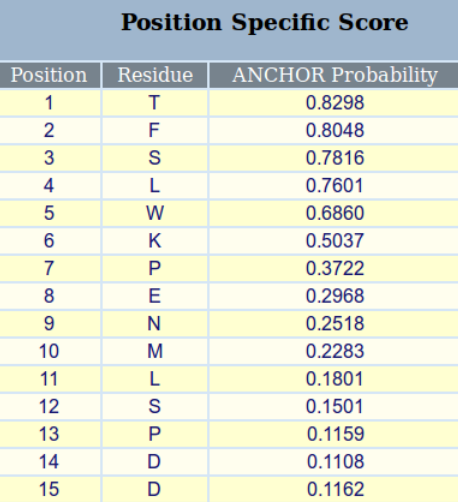
\includegraphics[width=0.5\textwidth]{img/anchorTabla.png} 
\caption{}
\label{anchorResults}
\end{figure}

Las posiciones 1-6 tienen asociados valores $>0.5$. Aplicando nuestro esquema de evaluación, estos resultados se traducen en la siguiente tabla de puntajes:

\vspace{0.5cm}
\noindent
\begin{tabular}{llllllllllllllll} 
\hline      
Secuencia & \textbf{T} & \textbf{F} & \textbf{S} & \textbf{L} & \textbf{W} & \textbf{K} & \textbf{P} & \textbf{E} & \textbf{N} & \textbf{M} & \textbf{L} & \textbf{S} & \textbf{P} & \textbf{D} & \textbf{D} \\ \hline
Evaluación con ANCHOR & 1 & 1 & 1 & 1 & 1 & 1 & 0 & 0 & 0 & 0 & 0 & 0 & 0 & 0 & 0\\ \hline
\end{tabular}


















\section{Otros propiedades evaluadas}

Como parte de la herramienta se provee la opción de realizar evaluaciones adicionales sobre la secuencia que permiten restringir la búsqueda más allá de las propiedades intrínsecas que debe poseer una secuencia linker.
Las distintas características ``extras'' que se permite definir sobre la secuencia complementan el objetivo principal de la herramienta que es proveer secuencias que puedan ser utilizadas 
en el contexto de desarrollos experimentales de biología molecular.
% distintas propiedades de la secuencia que, si bien no hacen directamente a su funcionalidad como linker, 
% complementan las características de la herramienta y 
% el objetivo de las secuencias resultantes como productos que serán utilizados 

Estas opciones, al no formar parte del conjunto de propiedades evaluadas de forma estándar, se debe indica su aplicación mediante parámetros al iniciar la ejecución, tal como se indica en la sección \ref{evaluacion} del manual.

\subsection{Carga neta de la secuencia}

% Otro de los motivos por las cuales se podría querer eliminar aminoácidos cargados es cuando se esta diseñando una proteína que se une a dna porque los residuos del linker podrían 
% entonces formar puentes salinos con los fosfatos del dna

Para evaluar una secuencia con respecto a la carga neta se tienen en cuenta tres categorias de aminoácidos: con carga positiva (K,R,H), carga negativa (E,D) y neutros.
Al evaluar una secuencia, primero se evalua la carga neta de esta lo que puede dar 3 casos:

\begin{itemize}
  \item Si la carga neta objetivo y la actual son iguales, todos los puntajes serán 0.
 
\item Si la carga neta a la que se está apuntando es más positiva que la actual, los puntajes resultantes son: 
  \begin{itemize}
   \item  aminoácidos con carga negativa = 2
  \item aminoácidos con carga positiva = 0
  \item aminoácidos neutros = 1
  \end{itemize}
Por ejemplo, si se está evaluando la secuencia \texttt{VKTCLALGVDI} (carga neta=0), y el usuario indicó como requerimiento una carga neta objetivo igual a +2, 
   
 
 \vspace{0.5cm}
\begin{center}
  \begin{tabular}{llllllllllllllll} 
\hline

Secuencia & \textbf{V} & \textbf{K} & \textbf{T} & \textbf{C} & \textbf{L} & \textbf{A} & \textbf{L} & \textbf{G} & \textbf{V} & \textbf{D} & \textbf{I} \\ \hline
Evaluación carga neta & 1 & 0 & 1 & 1 & 1 & 1 & 1 & 1 & 1 & 2 & 1  \\ \hline
\end{tabular}
\end{center}

 
 \item Si la carga neta a la que se apunta es más negativa que la actual, los puntajes resultantes son:
  \begin{itemize}
   \item  aminoácidos con carga negativa = 0
  \item aminoácidos con carga positiva = 2
  \item aminoácidos neutros = 1
  \end{itemize}

   Por ejemplo, si se está evaluando la secuencia \texttt{VKTCLALGVDI} (carga neta=0), y el usuario indicó como requerimiento una carga neta objetivo igual a -2:
   
   \vspace{0.5cm}

   \begin{center}
\begin{tabular}{llllllllllllllll} 
\hline
Secuencia & \textbf{V} & \textbf{K} & \textbf{T} & \textbf{C} & \textbf{L} & \textbf{A} & \textbf{L} & \textbf{G} & \textbf{V} & \textbf{D} & \textbf{I}\\ \hline
Evaluación carga neta & 1 & 2 & 1 & 1 & 1 & 1 & 1 & 1 & 1 & 0 & 1  \\ \hline
\end{tabular}

   \end{center}
   
\end{itemize}





\subsection{Absorción UV}

El objetivo de esta opción es que la secuencia resultante no posea ningún aminoácido que absorba en el rango del UV (W,Y,F).
En este caso, ya que se espera que el resultado final NO posea ninguno de estos residuos, directamente se eliminan de la composición de aminoácidos que se utiliza para reemplazar las posiciones mutadas. 
% Es decir, al momento de hacer las mutaciones, los residuos T,Y,F poseerán una frecuencia de s
Para eliminar los residuos que se encuentran en la secuencia, se asigna un puntaje de 1 a aquellas posiciones que contengan residuos absorbentes en el rango UV. 
Por ejemplo, si estamos evaluando la secuencia \texttt{VYTCLALGWDI}:

  \vspace{0.5cm}

\begin{center}
\begin{tabular}{lcccccccccccccc} 
\hline
Secuencia 	& \textbf{V} & \textbf{Y} & \textbf{T} & \textbf{C} & \textbf{L} & \textbf{A} & \textbf{L} & \textbf{G} & \textbf{W} & \textbf{D} & \textbf{I}\\ \hline
Evaluación UV 	& 0 & 1 & 0 & 0 & 0 & 0 & 0 & 0 & 1 & 0 & 0  \\ \hline
\end{tabular}
\end{center}











% 
% \section{Ejemplo completo de evaluación}
% 
% Esta secuencia linker (que se encuentra en las posiciones 202-284) une 2 dominios de la Regulatory protein E2 (del Human papillomavirus type 16):
% Un dominio es el TRANSACTIVATION DOMAIN (posiciones 1-201), el otro es el DNA-BINDING DOMAIN (posiciones 285-365),
% 
% 
% \resizebox{1.2\linewidth}{!}{
% \hspace{-1.5cm}
% \begin{tabular}{ccccccccccccccccccccccccccccccccccccccccccccccccccccccccccccccccccccccccccccccccccccc}
% algo&N&E&V&S&S&P&E&I&I&R&Q&H&L&A&N&H&P&A&A&T&H&T&K&A&V&A&L&G&T&E&E&T&Q&T&T&I&Q&R&P&R&S&E&P&D&T&G&N&P&C&H&T&T&K&L&L&H&R&D&S&V&D&S&A&P&I&L&T&A&F&N&S&S&H&K&G&R&I&N&C&N&S&N \\ \hline
% \end{tabular}
% }
% 









% DOCUMENTACION
\chapter{Manual de uso}\label{manual}


\section{Parámetros de ejecución}\label{parametros}

% El conjunto de parámetros corresponde al , no todos los parámetros serán parte de la versión publica en el servidor

\subsection{Secuencia inicial} \label{secuenciaInicial}
\subsubsection{Secuencia inicial random}\label{secuenciaInicialRandom}
Por default (si no se agrega ningún parámetro), la secuencia inicial se generará una secuencia random con la composición designada para la ejecución (ver \ref{composicion}).\\
Por default esta secuencia tendrá una longitud inicial = 10 AAs.

La longitud(en número de residuos) de esta secuencia inicial puede ser definida por el usuario mediante el parámetro \texttt{length} de la forma: \\
\indent \texttt{--length [seq-length]}
\\Por ejemplo: \\
\indent \texttt{--length 30} \hspace{0.5cm} Inicia la ejecución con una secuencia random de largo = 30 AAs


\subsubsection{Secuencia inicial definida}\label{secuenciaInicialDefinida}
Para definir una secuencia inicial especifica se debe usar el parámetro \texttt{seq} de la forma: \\
\indent \texttt{--seq [secuencia]} 
\\Por ejemplo: \\
\indent \texttt{--seq AAHHWWWLLLLHHGGG} \hspace{0.5cm} Inicia la ejecución con la secuencia \texttt{AAHHWWWLLLLHHGGG}

En caso de especificarse una secuencia inicial no es necesario definir longitud y, si se define, es ignorada.

\subsection{Composición de la secuencia} \label{composicion}

% Existen dos opciones para definir la composición usada durante la ejecución del método.
Si no se define ningún parametro al respecto, la composición \textit{default} que se usa es la composición estándar obtenida de SwissProt \cite{compositionAA}.  

Es posible también definir una composición a medida

\subsection{Evaluación de la secuencia}\label{evaluacion}

\subsection{Condición de finalización} \label{condicionFin}

\subsection{Formato y detalles del resultado}\label{output}
Los parámetros que permiten modificar el formato de la salida son:
\vspace{0.2cm}\\
\texttt{--verbose} \\
\indent \indent Devuelve una salida detallada de la ejecución \\
\texttt{--minoutput} \\
\indent \indent Solo devuelve el resultado final y guarda el historial de mutaciones en un log \\
\texttt{--stepped} \\
\indent \indent Espera por input del usuario en cada paso del método. \\


% EVALUACION DE LA HERRAMIENTA Y RESULTADOS
\chapter{Evaluaciones y análisis de resultados}
\label{results}

\section{Parámetros de ejecución}

Todas las evaluaciones se realizaron con los parámetros estándar del método descritos en el manual (ver capítulo \ref{manual}).
El equipamiento y software utilizado para las pruebas se encuentra descrito en el apéndice \ref{equipamiento}.

\section{Estimación del parámetro Beta}\label{betaResults}
% PRIMERO EXPLICAR COMO DEPENDE LA EJECUCION CON EL PARÁMETRO BETA
% PARA VALORES MAS CHICOS ...
% PARA VALORES MAS GRANDES...
% DAR UNA IDEA DEL RANGO DE VALORES BETA DE ACUERDO A LA ECUACION, PARA DIFERENCIAS DE SCORE = 1
% MOSTRAR GRAFICO/S DE RELACION ENTRE 
% POR LO TANTO, UN PARAMETRO QUE TIENE EN CUENTA ESTOS ASPECTOS, QUE PODRIA EVALUAR CORRECTAMENTE LA EJECUCION EN FUNCION DE BETA , Y QUE ADEMAS ES EL DATO MAS IMPORTANTE EN LA EJECUCION ES EL TIEMPO DE EJECUCION

En las secciones previas hemos propuesto un método de diseño que se basa en búsqueda estocástica sobre el espacio de secuencias.
El método de búsqueda es guiado por el resultado de una función que asigna un puntaje a cada secuencia, el cual resulta siempre mayor o igual a 0.
La secuencia resultante buscada se caracteriza por tener un puntaje igual a 0, por lo tanto, el método puede verse como la búsqueda de un mínimo global sobre la superficie
que relaciona cada posible secuencia con su valor de puntaje.
% El el valor(o el rango) óptimo para el parámetro que Beta depende en gran parte de las características de esta superficie.

El comportamiento del método de búsqueda depende de un único parámetro $\beta$ cuyo valor (o rango) óptimo está fuertemente asociado a las características de esta superficie.
Un valor de $\beta$ más grande tiene un porcentaje de aceptación mayor de mutaciones que aumentan el puntaje de la secuencia, por lo tanto, permite la exploración de superficies que 
requieren superar mínimos locales para alcanzar secuencias con puntaje 0.
Un valor de beta mas chico implica recorrer un camino más directo hacia el mínimo ya que se aceptan menos mutaciones que aumenten el puntaje, pero esto podría requerir la evaluación de una gran cantidad de posibilidades. 
Incluso, si la búsqueda se estanca en un mínimo local, un valor muy chico de beta solo podría encontrar la solución en un tiempo infinitamente 
grande. Como vimos en el capítulo 2, la decisión de aceptación está basada en el uso de la ecuación \ref{monteCarlo}, la cual siempre devuelve un valor $>0$ para cualquier $\beta$ positivo.
% Para cualquier valor de $\beta$ positivo dadas las propiedades del método de decisión para aceptar las mutaciones,   el valor de la ecuación \ref{monteCarlo} siempre será mayor que 0. 
Por lo tanto, la probabilidad de aceptación nunca es 0 y no es imposible encontrar el resultado si es que existe, aún cuando el tiempo que se demore sea prácticamente infinito.

% En esta aplicación, además, partiendo de una secuencia inicial dada por el usuario, resultaría mejor obtener la secuencia con puntaje mínimo que esté más cerca en la superficie, es decir, que sea más similar a la secuencia inicial.
% Esto implica una menor cantidad de mutaciones, lo que equivale a un valor de beta mas chico.

A pesar que, previo a desarrollar la aplicación asumimos que el espacio de soluciones era considerablemente grande, no sabemos cómo es exactamente 
la superficie que asocia cada secuencia con el puntaje definido por las evaluaciones. 
De esta forma, inicialmente no tenemos ningún conocimiento de como se relaciona el valor del parámetro $\beta$ con la ejecución
resultante, ni cuales serán los valores de $\beta$ que nos permitirán obtener diseños de la forma más eficiente.
% Sin embargo, no sabemos como estos intentos de encontrar mejores mutaciones afectan a la optimalidad de la búsqueda global.
% Para tener una primera idea global de esta dependencia analizamos e
% Todavía no sabemos las implicancias de realizar esta cantidad de intentos de mutacion sobre la búsqueda.
La forma más directa de conocer cual es el rango (o valor) óptimo de $\beta$ es mediante la evaluación del tiempo de ejecución, es decir, el tiempo total requerido para la búsqueda del diseño resultante. 
Para esto, se midió el tiempo de ejecución para distintas corridas que utilizan valores de beta en el rango 0.1-2.5.
% La evaluación realizada implicó la medición del tiempo de ejecución para distintas ejecuciones que utilizan valores de beta en el rango 0.1-2.5.
Puntualmente se analizan los valores en el conjunto (0.1, 0.5, 1.0, 1.5, 2.0, 2.3, 2.5). 
Se realizaron 6 ejecuciones para cada valor de $\beta$ analizado, de las cuales 3 se realizan a partir de secuencias definidas (obtenidas de proteínas naturales) y otras 3 a partir de secuencias generadas aleatoriamente.
En todos los casos con una longitud de 50 residuos.

En la figura \ref{fig:beta-vs-time} se muestran los tiempos medios asociados a cada conjunto de evaluaciones.
En primer lugar vemos que no hay una diferencia significativa constante entre las ejecuciones que inician a partir de secuencias naturales y las que lo hacen a partir de secuencias aleatorias.
% Al parecer, si bien las primeras pueden tener valores de score mayore
Por otro lado, se ve que el tiempo de ejecución es altamente variable para la mayoria de los valores de $\beta$.
Esta variabilidad, que se basa en las propiedades estocásticas de la búsqueda, no permite definir un valor óptimo puntual. Se puede ver, igualmente, que el tiempo de ejecución es significativamente mayor en el caso de $\beta$ muy grande (2.3 y 2.5), 
indicando que el rango óptimo de valores está ubicado hacia el extremo inferior.
Aunque el rango completo 0.1-2.0 es aceptable, definimos a $\beta=$1.0 como un valor que nos permitirá realizar la ejecución en un tiempo aceptable, quedando como valor estándar de la herramienta.



\begin{figure}[htbp]
% \advance\leftskip-1.2cm
% 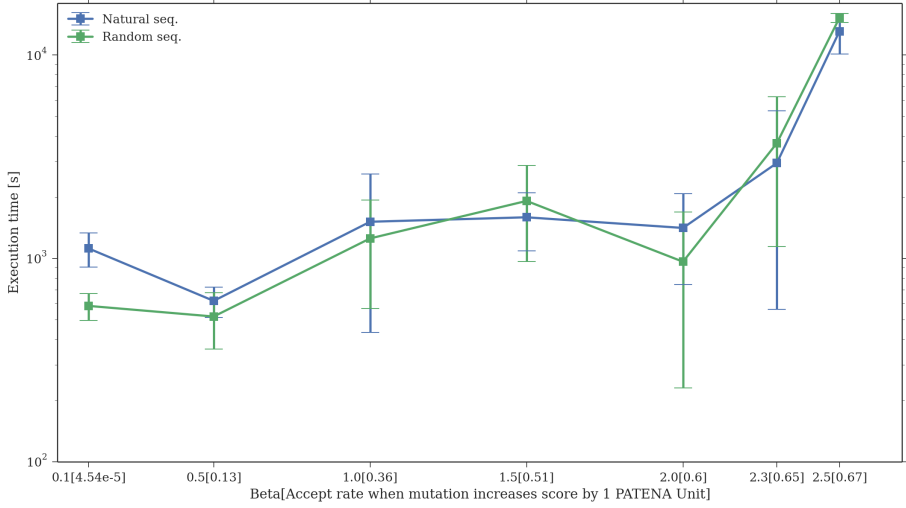
\includegraphics[width=1.1\textwidth]{img/resultados/beta-vs-time-length50-rate.png}
\centering
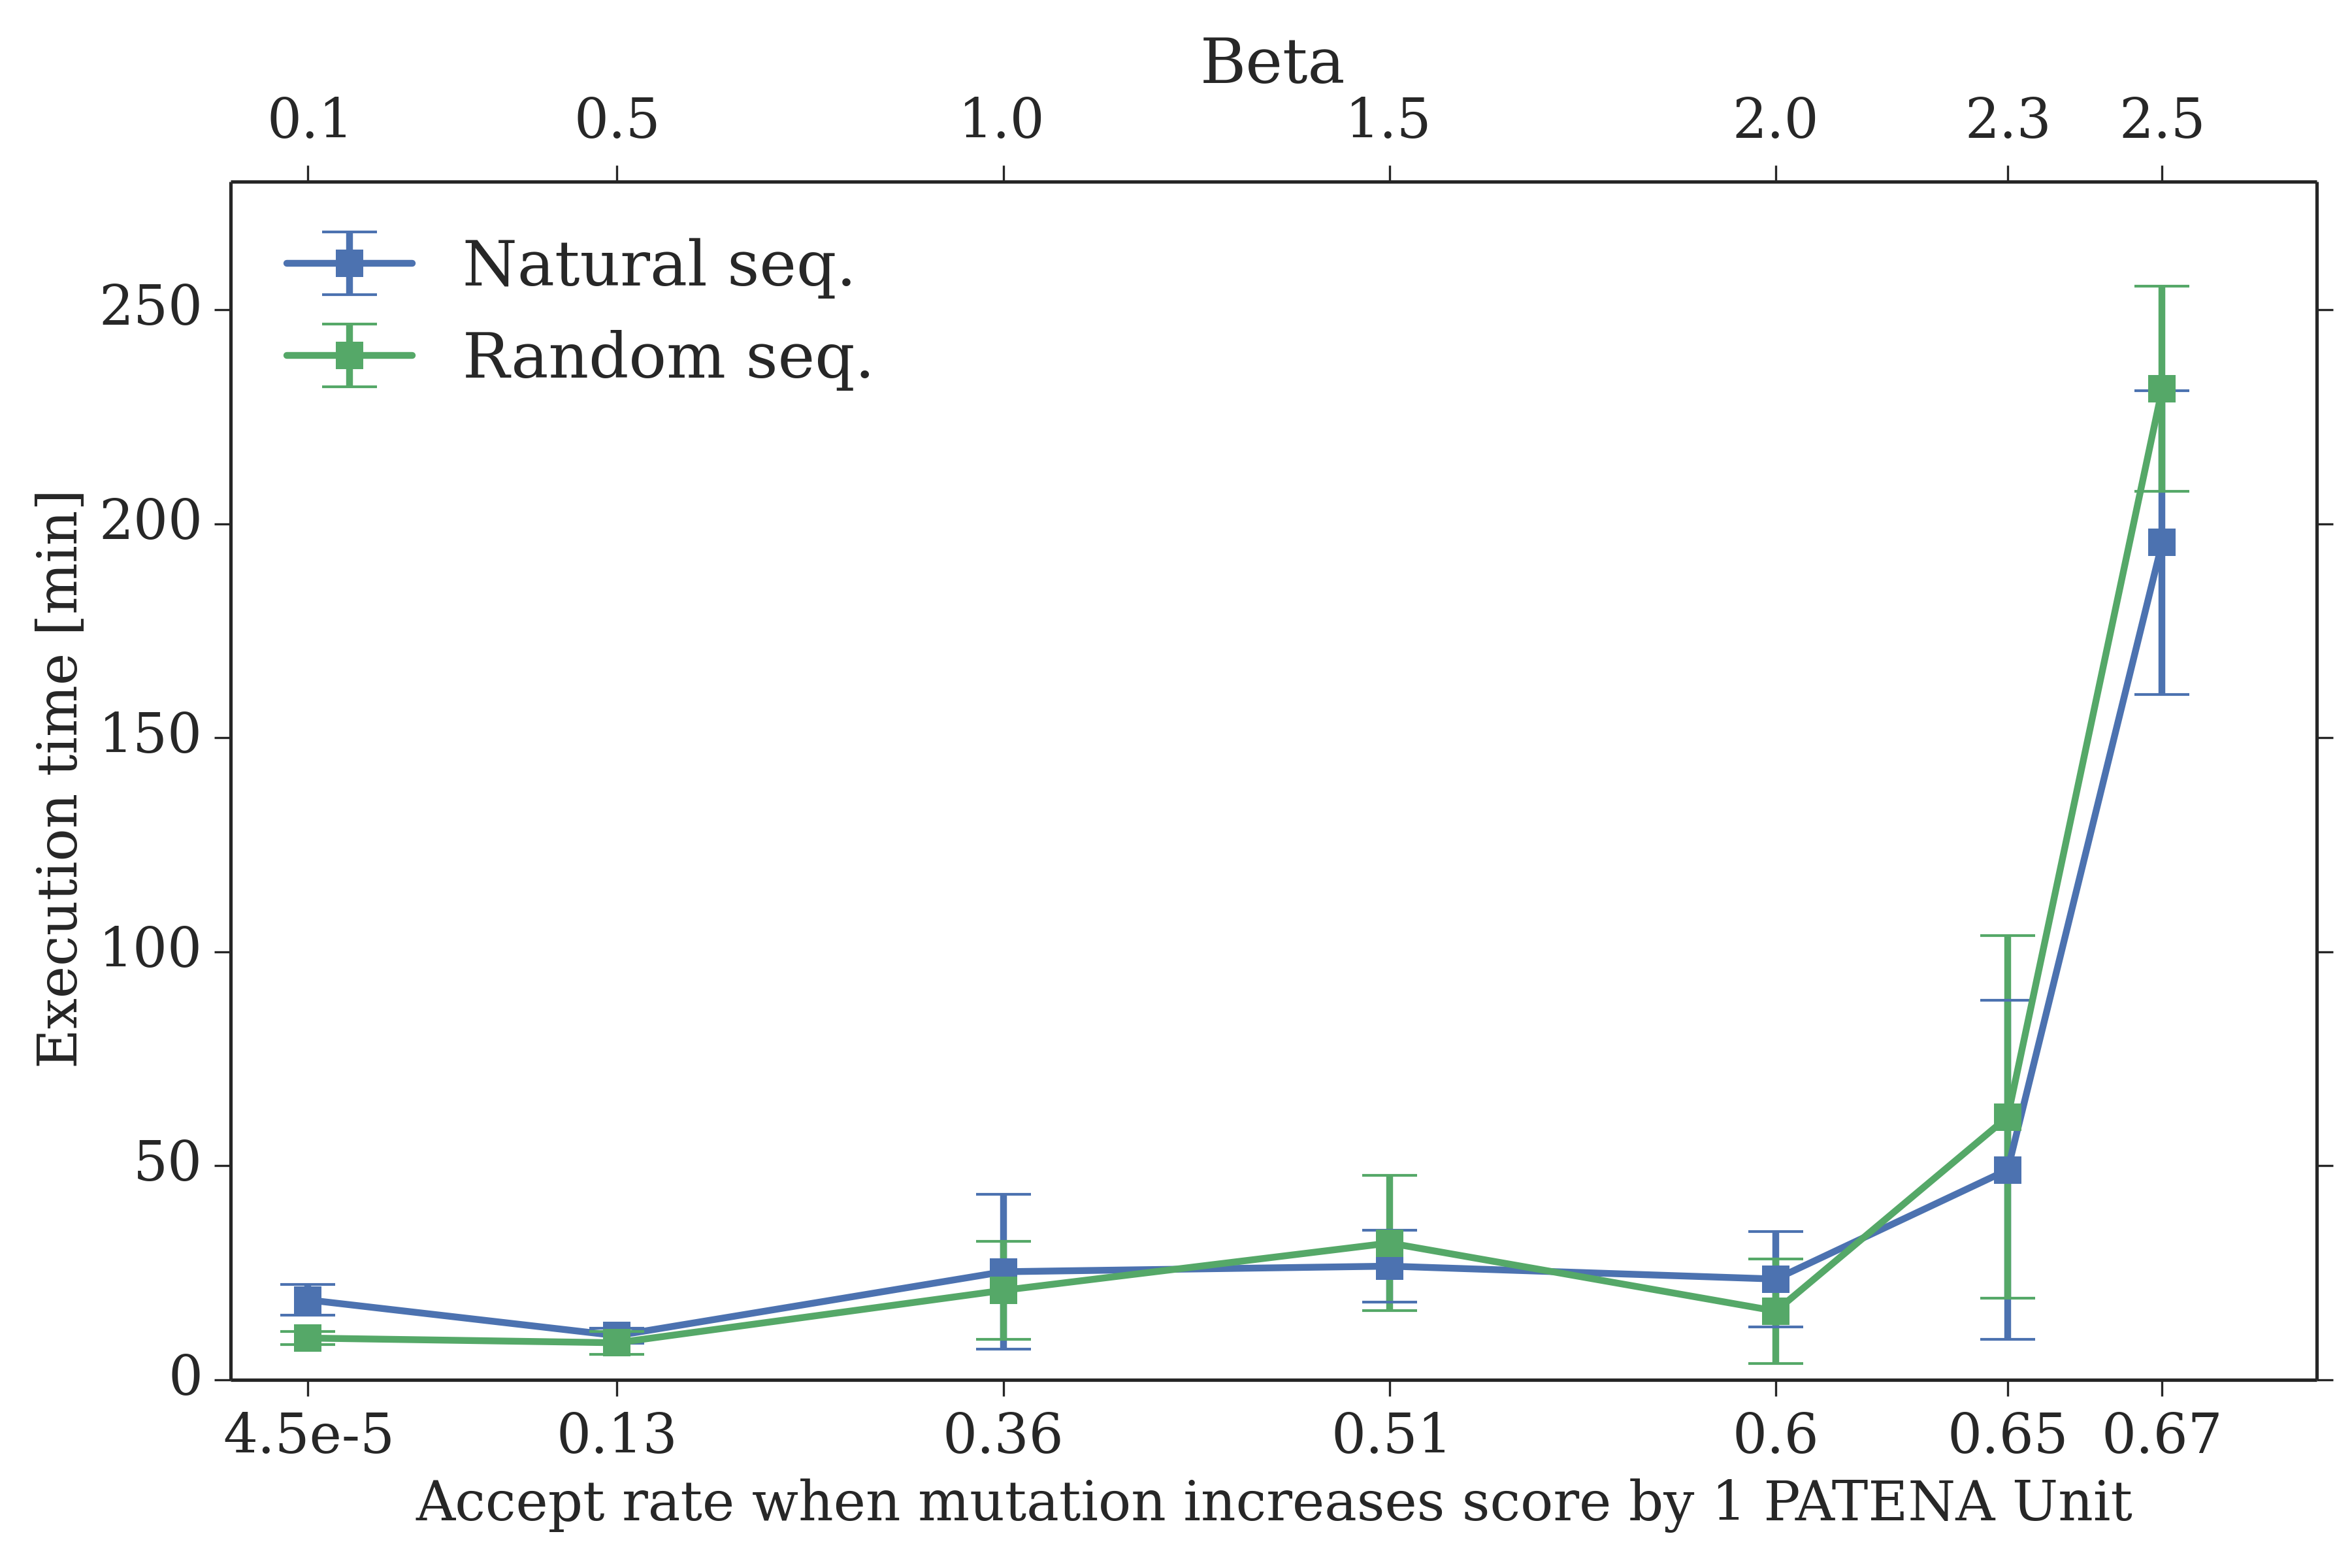
\includegraphics[width=0.9\textwidth]{img/resultados/beta-vs-time-length50-300dpi.png}
\caption{\textbf{Dependencia del tiempo de ejecución con beta}}
\label{fig:beta-vs-time}
\end{figure}



%************************ HASTA ACA ESTA BIEN ***********************












\section{Análisis detallado de la ejecución}
% ***************************************************************
% 
%    ACA LA IDEA ES DESGLOSAR LA DEPENDENCIA DEL TIEMPO CON BETA
% 



% Una vez definido el valor efectivo de $\beta$ queda completo el método listo para su utilización. 
% La estimación del valor de $\beta$ que provea un menor tiempo de ejecución nos permite conocer cual es el valor que provee un correcto balance entre la exploración y la explotación de la superficie.
El rango de $\beta$ obtenido es útil para poder encontrar resultados eficientemente pero, si queremos conocer más en detalle las propiedades de la búsqueda,
% detalle más sobre la superficie que estamos explorando, 
% pero para tener una idea más detallada del perfil de las ejecuciones, 
hace falta desglosar la ejecución.
Los detalles de las búsquedas permiten, además, inferir ciertas características de la superficie que se esta explorando.
Sabiendo que las propiedades de la búsqueda son, puntualmente, 
% Sabiendo que los tiempos de ejecución son producto directo de 
la cantidad total de mutaciones aceptadas y la cantidad de mutaciones que se intentan para cada ejecución, 
en lo que resta de esta sección analizaremos cómo cambian los perfiles de estas variables según el valor de beta. % en la búsqueda que estamos realizando.
% Sabemos que el tiempo de ejecución resultante es producto del número de mutaciones y de intentos de mutación, 
 
Para tener una primera idea de esta dependencia, analizaremos los perfiles de ejecución para dos valores puntuales de beta: $\beta=$0.5 y $\beta=$2.4.
En el caso del $\beta$ más chico (0.5), la probabilidad de aceptar una mutación para un incremento de 1 en el puntaje es de $13\%$, mientras que para el beta más grande (2.4) esta probabilidad es de $65,9\%$.
Por lo tanto, los dos valores podrían clasificarse como cercanos a los extremos dentro del esquema de decisión basado en el puntaje.
Para cada valor de $\beta$ se realizaron 6 corridas independientes.
% En los gráficos \ref{fig:scoreVsiter} y \ref{fig:mutAttemptsVsite} se muestran los resultados de 6 corridas independientes para cada uno de los valores de $\beta$ evaluados (0.5 y 2.4).
% El tiempo de ejecución resultante es producto de dos variables de l
La mitad de estas corridas se iniciaron a partir de secuencias generadas aleatoriamente, mientras que las restantes se inician a partir de secuencias naturales definidas (distintas entre si).
En todos los casos la longitud de la secuencia fue de 30 aminoácidos. Los resultados se muestran en las figuras \ref{fig:scoreVsiter} y \ref{fig:mutAttemptsVsite}.
% Este mismo esquema de 6 corridas se repitió para los dos valores de $\beta$ (0.5 y 2.4).
% En el caso del $\beta$ más chico (0.5), la probabilidad de aceptar una mutación para un incremento de 1 en el puntaje es de $13\%$, mientras que para el beta más grande (2.4) esta probabilidad es de $65,9\%$.
% Por lo tanto, los dos valores podrían clasificarse como cercanos a los extremos dentro del esquema de decisión basado en el puntaje.
% rango de posibles valores para $\beta$.
% Los resultados de las corridas se muestran en la tabla ......... ***CONVIENE RESUMIR BIEN LOS DATOS EN UNA TABLA? EL UNICO DATO CREO QUE SERIA EL TOTAL DE ITERACIONES




% 
% \begin{figure} 
% \advance\leftskip-2cm
% \subfigure[Ejecuciones individuales]{\label{fig:scoreVsiter-a}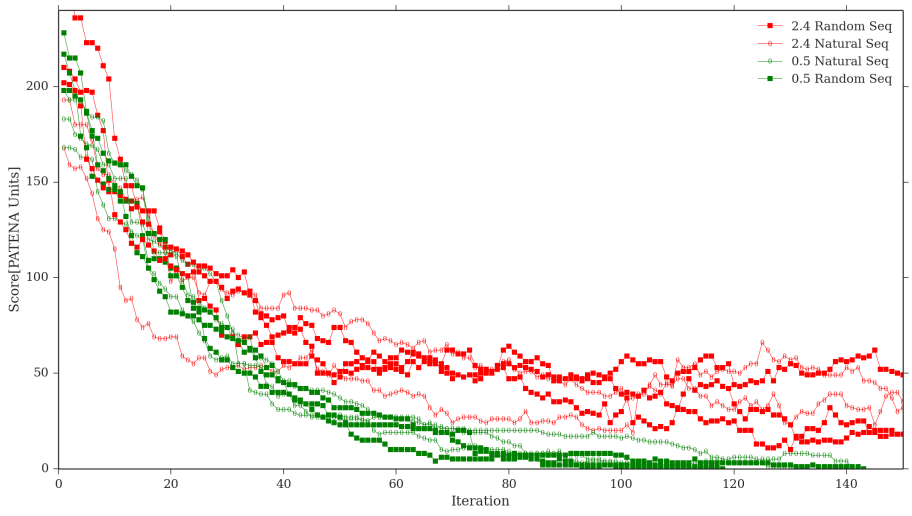
\includegraphics[width=1.15\textwidth]{img/resultados/individuales-scoreVsiter-hasta150.png}}
% \subfigure[Valores medios y desviaciones]{\label{fig:scoreVsiter-b}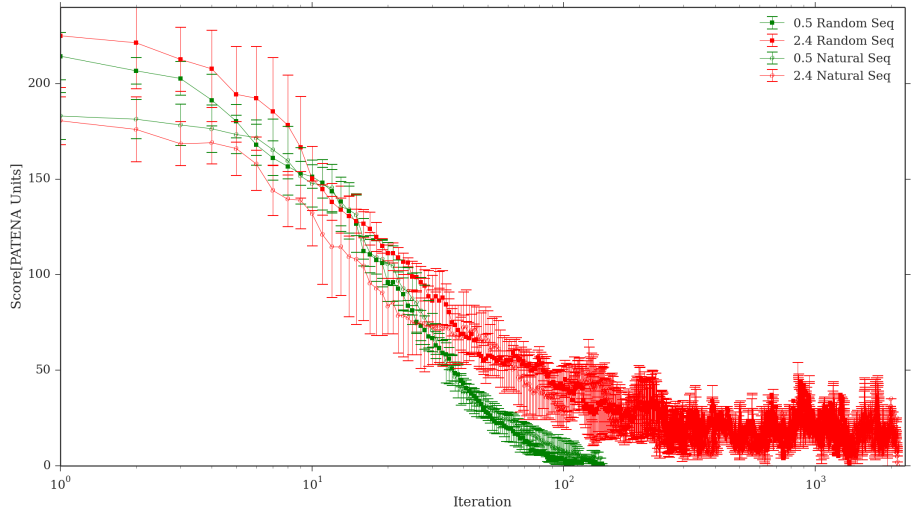
\includegraphics[width=1.15\textwidth]{img/resultados/scoreVsiter-cada1-hasta2270.png}}
%  \caption{Puntaje asociado a cada iteración}
%  \label{fig:scoreVsiter}
% 
% \end{figure}

% SCORE vs MUTACIONES  
\begin{figure}[htbp]
% \advance\leftskip-1.5cm
  \begin{subfigure}[b]{\textwidth}
%     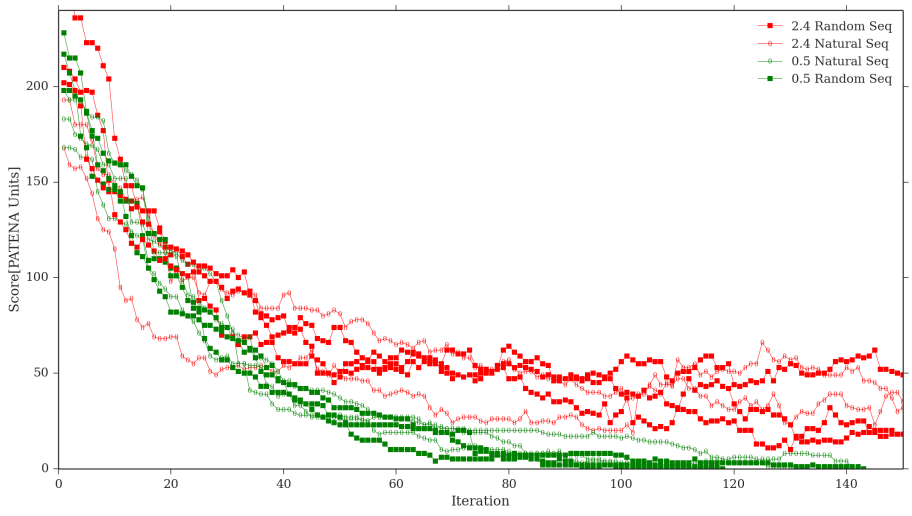
\includegraphics[width=1.15\textwidth]{img/resultados/individuales-scoreVsiter-hasta150.png}
 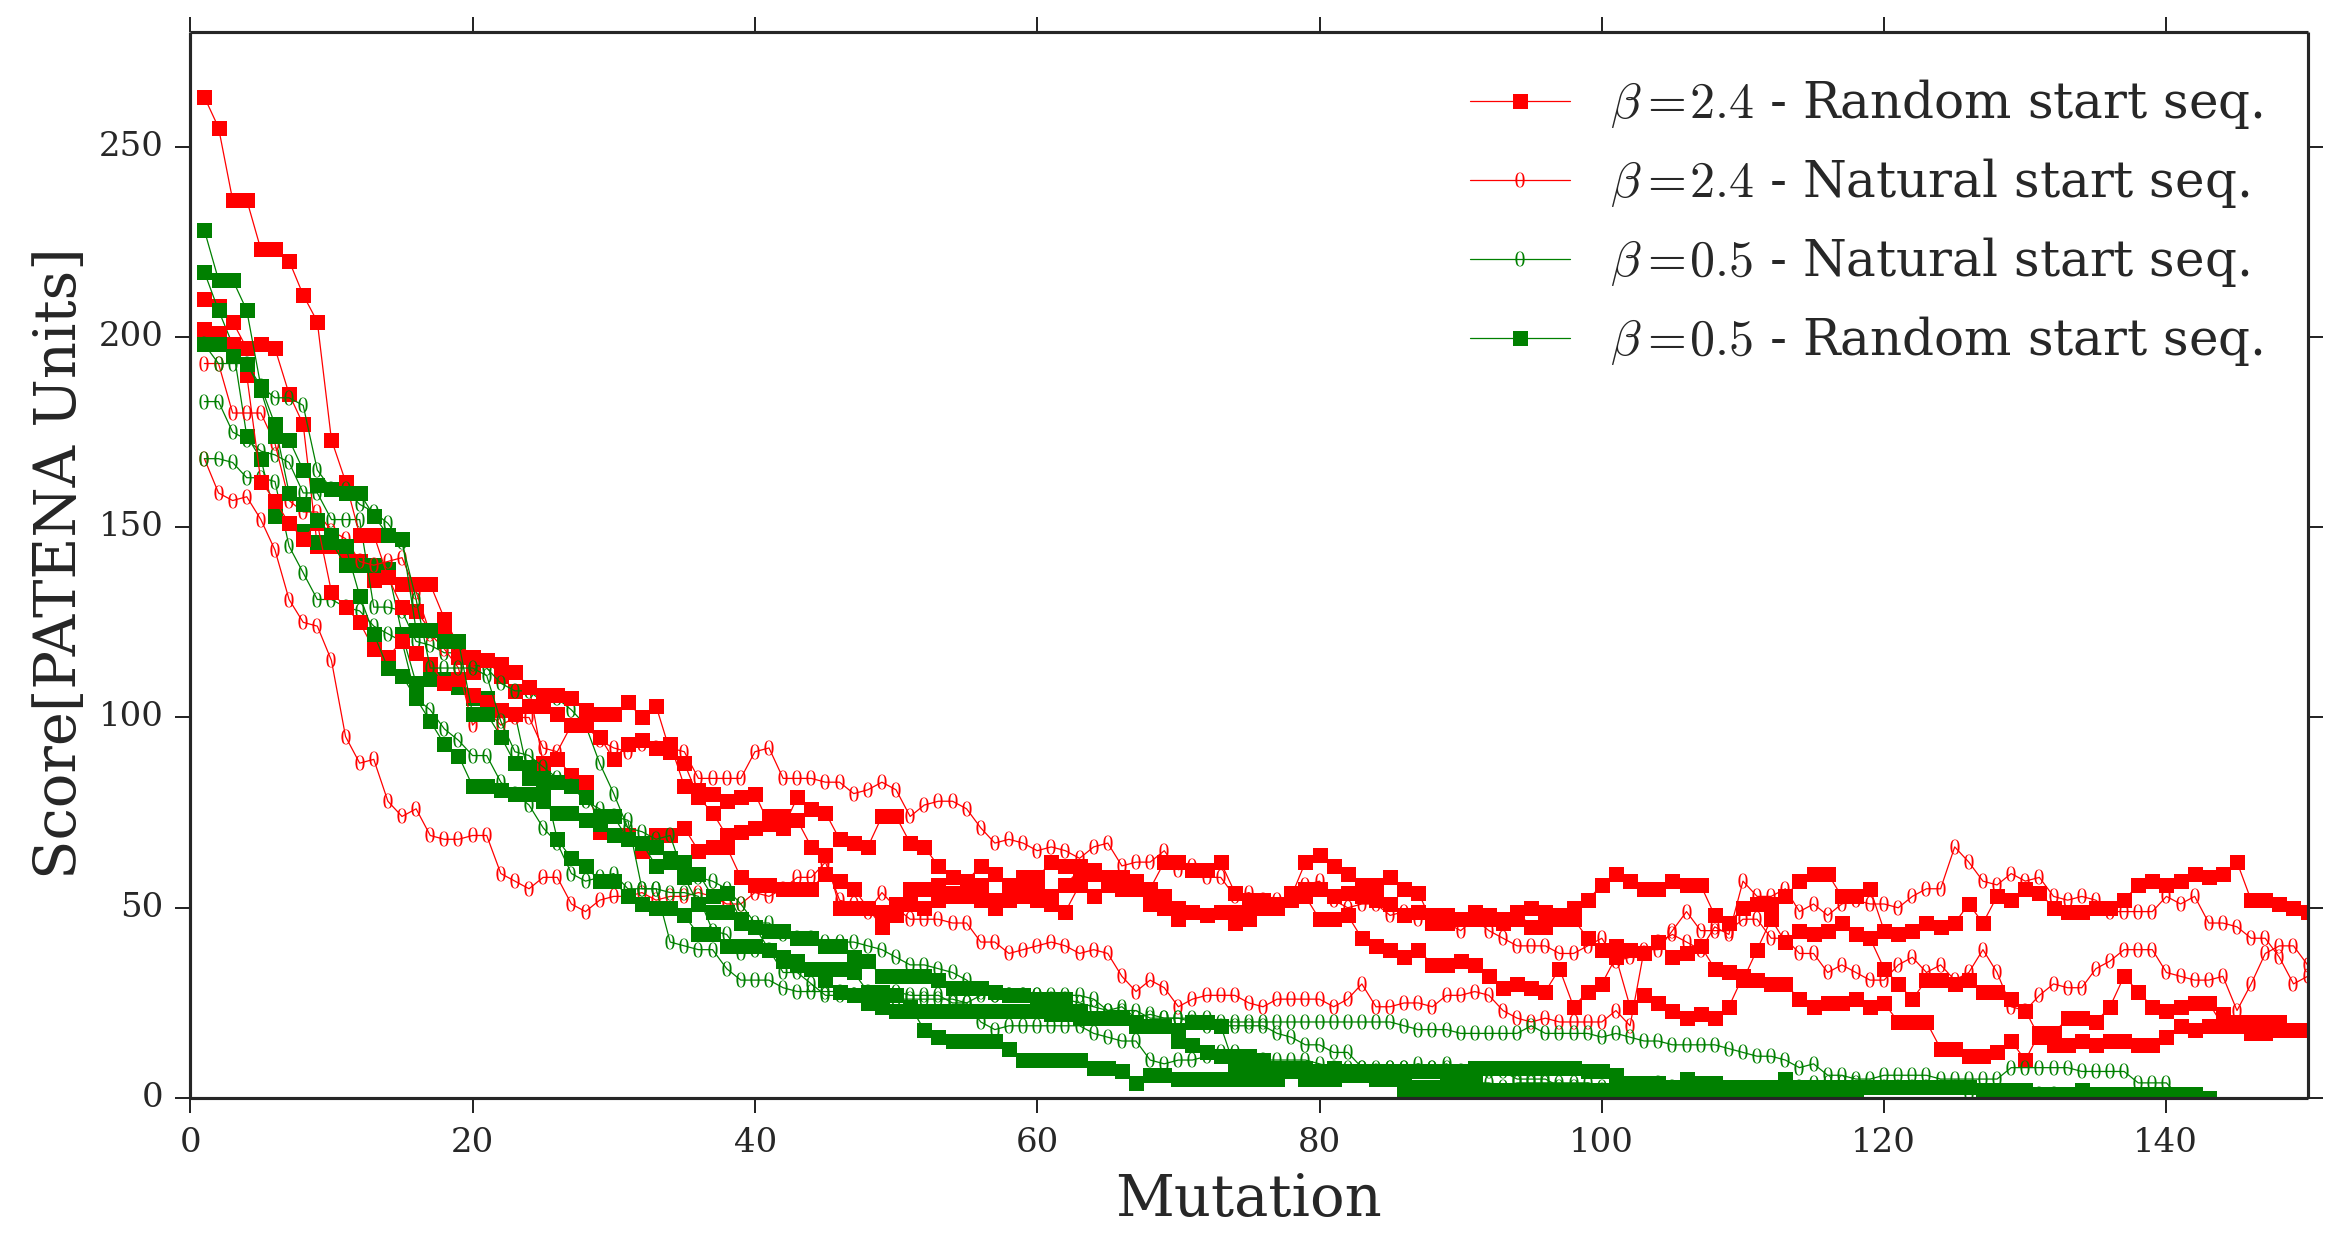
\includegraphics[width=\textwidth]{img/resultados/iterationVsScore-individual.png}
    \caption{Ejecuciones individuales}
    \label{fig:scoreVsiter-a}
  \end{subfigure}
%   \hspace{20px}
  \begin{subfigure}[b]{\textwidth}
%     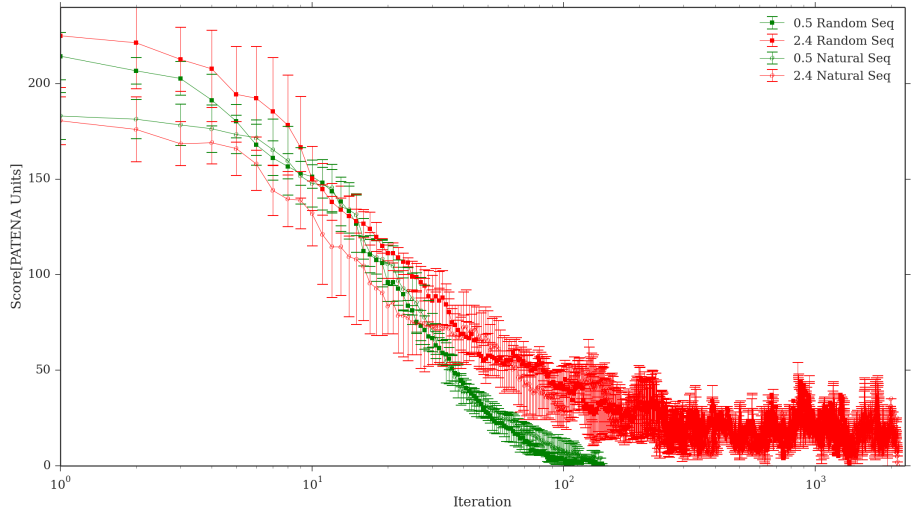
\includegraphics[width=1.15\textwidth]{img/resultados/scoreVsiter-cada1-hasta2270.png}
     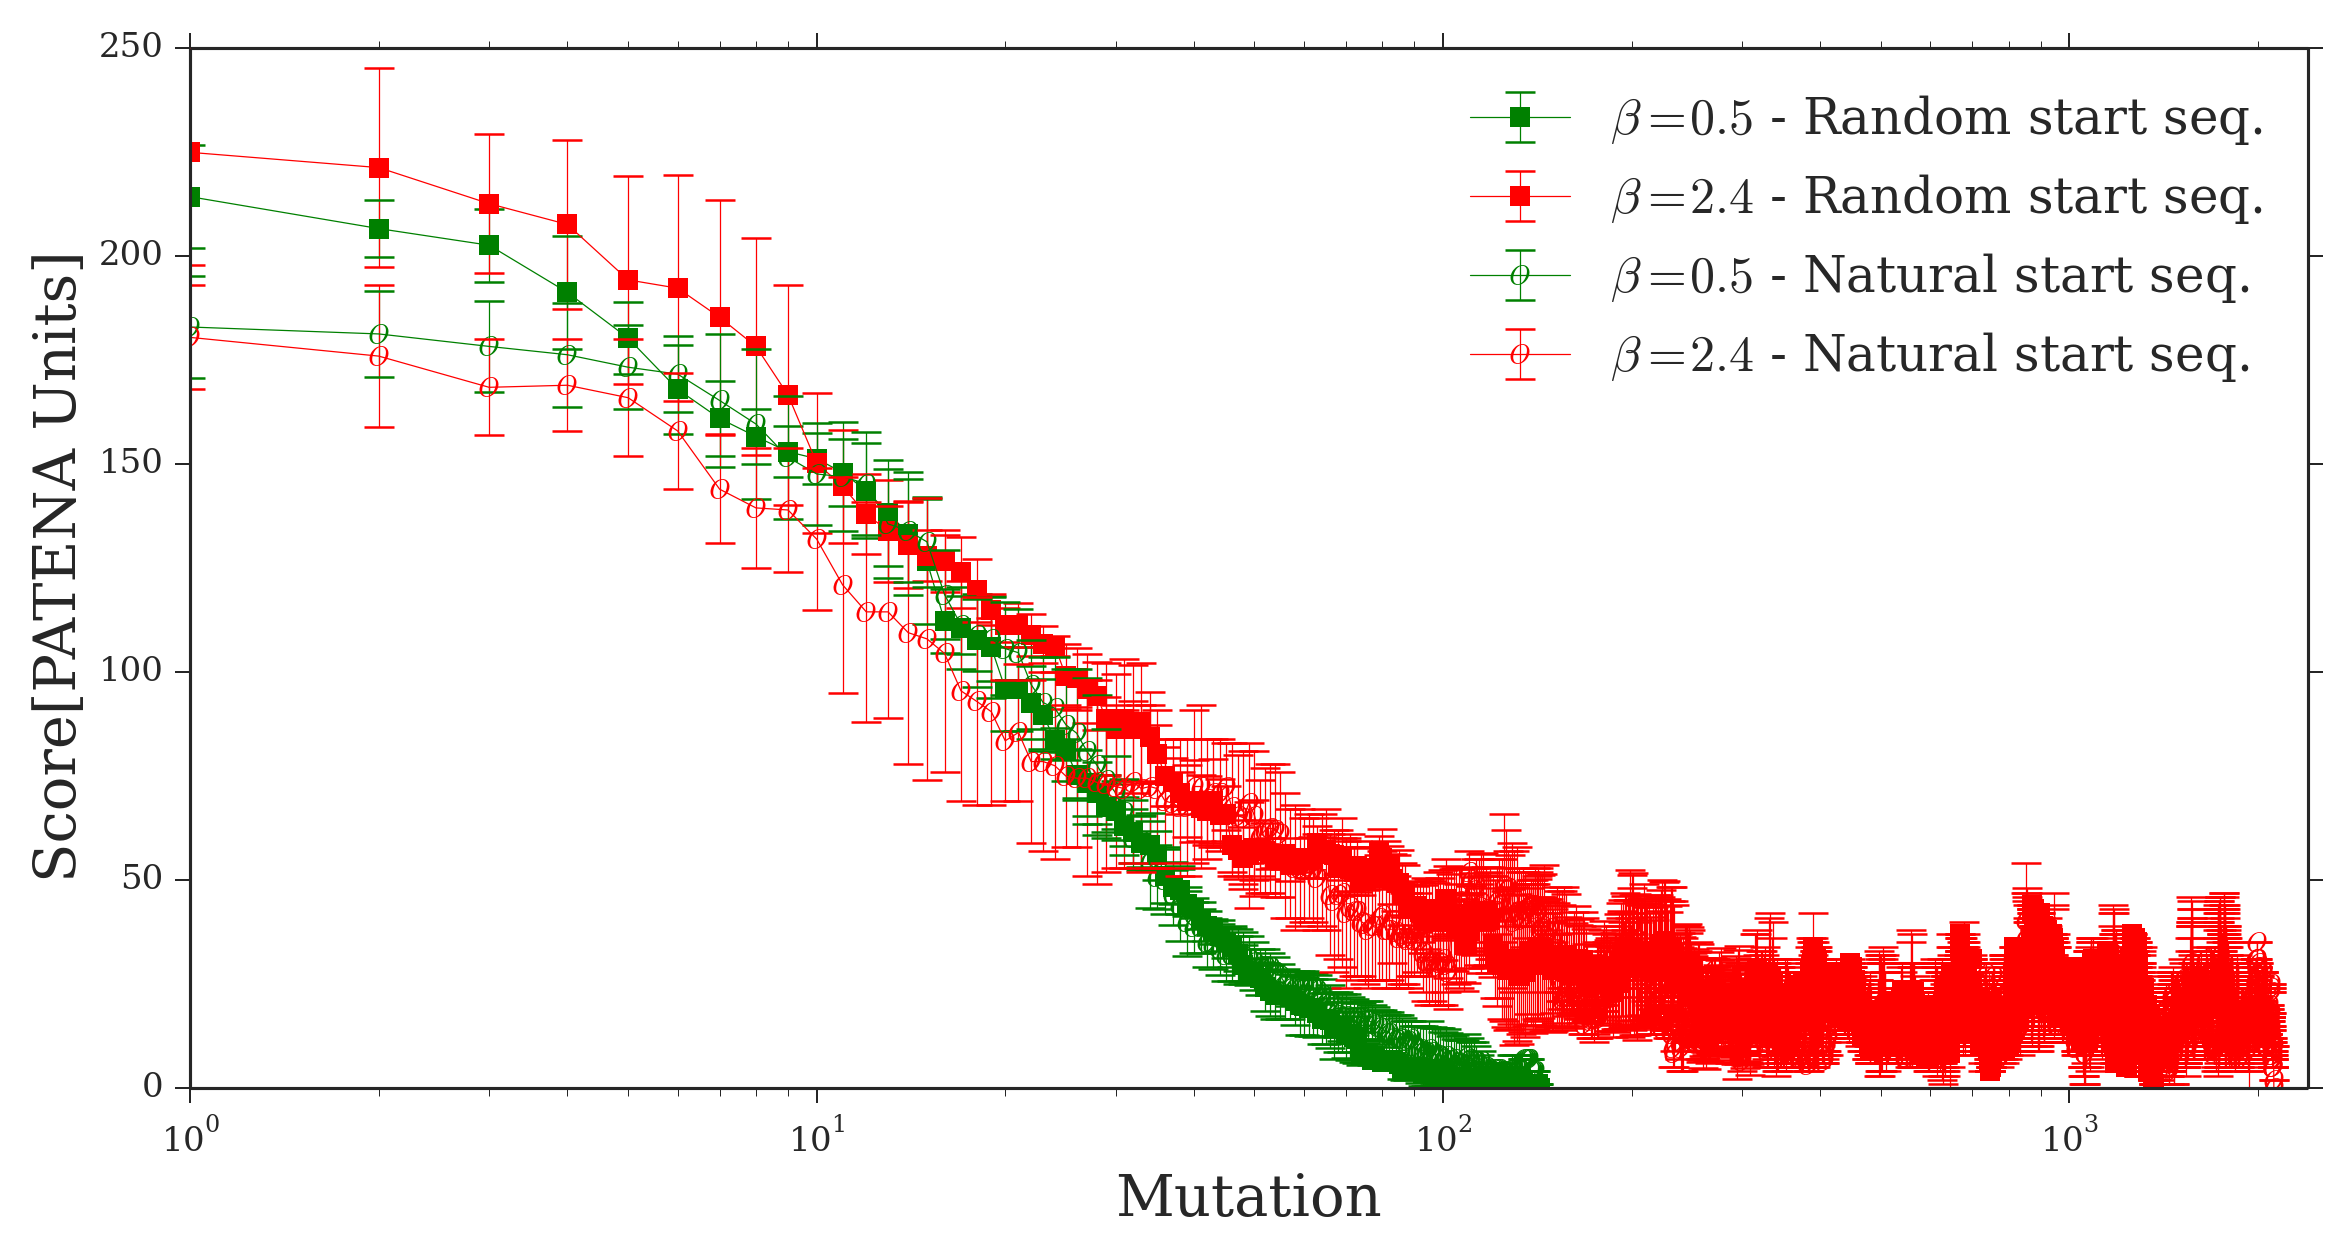
\includegraphics[width=\textwidth]{img/resultados/iterationVsScore-mean.png}
    \caption{Valores medios y desviaciones}
  \label{fig:scoreVsiter-b}
  \end{subfigure}
  \caption{\textbf{Perfil de puntajes asociado a cada iteración para distintos beta}}
  \label{fig:scoreVsiter}
\end{figure}




% \begin{figure} 
% \advance\leftskip-2cm
% \subfigure[Ejecuciones individuales]{\label{fig:mutAttemptsVsite-a}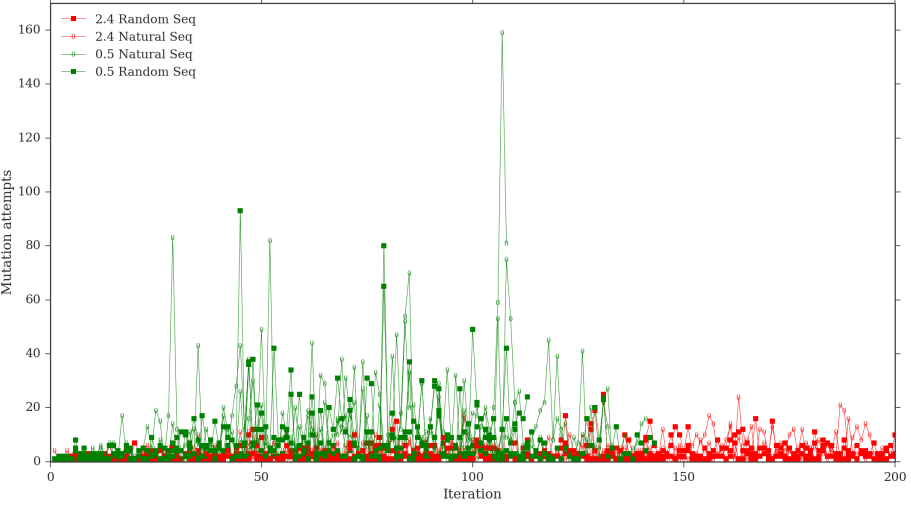
\includegraphics[width=1.15\textwidth]{img/resultados/individuales-mutAt-vs-iter-hasta200.png}}
% \subfigure[Valores medios y desviaciones]{\label{fig:mutAttemptsVsite-b}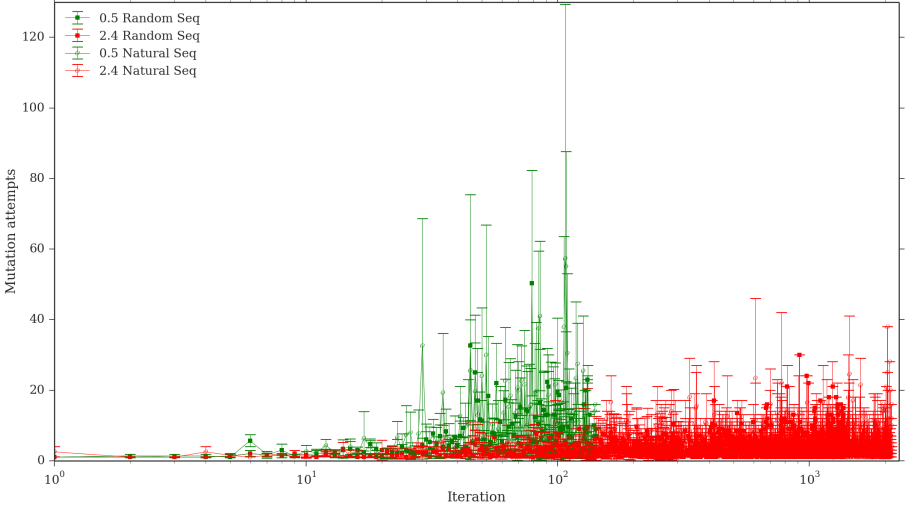
\includegraphics[width=1.15\textwidth]{img/resultados/mutAttemptsVsite-cada1-hasta2270.png}}
% \caption{Dependencia del número de intentos de mutación con la iteración}
% \label{fig:mutAttemptsVsite}
% \end{figure}


% INTENTOS DE MUTACION PARA BETA  0.5 Y 2.4
\begin{figure}[htbp]
% \advance\leftskip-1.5cm
  \begin{subfigure}[b]{\textwidth}
%     \includegraphics[width=1.15\textwidth]{img/resultados/individuales-mutAt-vs-iter-hasta200.png}
    \includegraphics[width=\textwidth]{img/resultados/iterationVsMutAttempts-individual.png}
    \caption{Ejecuciones individuales}
    \label{fig:mutAttemptsVsite-a}
  \end{subfigure}
%   \hspace{20px}
  \begin{subfigure}[b]{\textwidth}
%     \includegraphics[width=1.15\textwidth]{img/resultados/mutAttemptsVsite-cada1-hasta2270.png}
      \includegraphics[width=\textwidth]{img/resultados/iterationVsMutAttempts-mean.png}
    \caption{Valores medios y desviaciones}
  \label{fig:mutAttemptsVsite-b}
  \end{subfigure}
  \caption{\textbf{Dependencia del número de intentos de mutación con beta}}
  \label{fig:mutAttemptsVsite}
\end{figure}









% GRAFICO DE SCORE vs ITERACION   (MEDIAS Y StdDeV COMPLETO HASTA EL FINAL)   +  CORRIDAS INDIVIDUALES
En el gráfico \ref{fig:scoreVsiter} se muestra la dependencia del puntaje con las iteraciones, tanto los valores medios (y desviaciones estándar) para todas las ejecuciones mencionadas (gráfico \ref{fig:scoreVsiter-b}), 
como el detalle de las ejecuciones individuales (gráfico \ref{fig:scoreVsiter-a}).
El perfil que se muestra permite aclarar mejor los conceptos mencionados previamente acerca de la dependencia de $\beta$ con el comportamiento de la búsqueda. 
Un valor más grande de $\beta$ realiza una mayor exploración del espacio de soluciones, lo que se ve reflejado en un rango mucho más amplio de mutaciones aplicadas para alcanzar el resultado.
Se ve claramente que hay una diferencia en el orden de magnitud de la cantidad de iteraciones, donde las ejecuciones con $\beta=$2.4 pueden alcanzar más de 2000 iteraciones.
Por su parte, el valor más chico de $\beta$ permite alcanzar el objetivo en un número mucho menor de mutaciones, lo cual parece indicar que hay un camino 
que conduce desde cada punto de inicio hacia un resultado bajando continuamente el valor del puntaje, es decir, sin atravesar ninguna barrera.
De todas formas, no podemos decir nada sobre las características de este recorrido hacía el mínimo.
% PONER ALGUNA CONCLUSION DE QUE DICE ESTO ACERCA DE LA SUPERFICIE 

% Esta es, sin embargo, una visión muy general de la ejecución, y para tener una idea mas detallada es necesario analizar otros parámetros relevantes.
% y   MUT-ATTEMPTS vs ITERACION (MEDIAS Y StdDeV COMPLETO HASTA EL FINAL)   +  CORRIDAS INDIVIDUALES
En el gráfico \ref{fig:mutAttemptsVsite} se muestra el número de intentos de mutación asociado a cada valor de $\beta$.
Nuevamente se muestran los valores medios (y sus desviaciones correspondientes) en el gráfico \ref{fig:mutAttemptsVsite-b}, y el detalle de las ejecuciones individuales (gráfico \ref{fig:mutAttemptsVsite-a}).
Vemos que el reducido número de iteraciones que resulta de un valor bajo de $\beta$ se produce a costa de una cantidad más elevada de intentos de mutaciones, es decir, se evalúa una mayor cantidad de posibles mutaciones hasta 
que eventualmente una sea aceptada, lo que representa la dificultad del camino hacia el valor mínimo buscado. 
Esta condición se incrementa en las iteraciones cercanas al fín de la ejecución, que se corresponden con los valores más bajos de puntaje (cercanos a 0). 




% basicamente tengo que decir que los tiempos de ejecucion vistos son el resultado del balance entre el numero de intentos de mutacion y el numero de iteraciones totales.

Comprobamos, entonces, que un valor más grande de beta implica un incremento considerable en el número de mutaciones requeridas, aunque un valor menor de beta tendrá una mayor cantidad de intentos de mutacion por iteración.
Sabiendo que ambas propiedades impactan negativamente en el proceso de búsqueda incrementando el tiempo de ejecución, 
intentaremos ver ahora cómo, en el rango efectivo de beta, se crea el balance óptimo entre estos parámetros.
% ancean correctamente en el rango efectivo de beta descrito previamente.
% el rango efectivo de beta es producto del balance correcto entre estas propiedades.
% FALTA UNA CONEXION DE LAS EVALUACIONES PREVIAS (PARA BETA 0.5 Y 2.4) CON ESTO NUEVO,  
% Ahora tenemos una idea más clara de cómo afecta beta a los parámetros de exploración. 
% veremos cómo estos parametros se balancean
% intentaremos ver ahora cómo es el balance de estos parámetros con respecto a los distintos valores de beta, para dar los tiempos de ejecución vistos previamente.
% Trataremos de explicar los valores de tiempo de ejecución y el rango efectivo de beta encontrados previamente, basándonos en los parámetros de la búsqueda.
% Es decir, intentaremos explicar cómo la suma entre el número total de mutaciones y de intentos de mutacion producen los tiempos de ejecución encontrados. 
Para esto, analizaremos el perfil completo de las ejecuciones realizadas en la sección previa para encontrar el rango óptimo de beta, 
lo cual se muestra en las figuras \ref{fig:betaVsMut-AttemptsPerit} y \ref{fig:betaVsMutations-Attempts} (no se realiza la separación entre ejecuciones iniciadas a partir de secuencias naturales o secuencias random).

% ACA EMPIEZO A HABLAR DE LOS GRAFICOS DE VALORES  vs RANGO DE BETA:  intentos de mutacion, iteraciones , intentos de mutacion por iteracion
Lo que vemos en la figura \ref{fig:betaVsMut-AttemptsPerit} es que el número de intentos de mutación por iteración baja al aumentar el valor de $\beta$, lo cual es esperable de acuerdo a lo visto previamente.
Sin embargo, según se puede ver en el gráfico \ref{fig:betaVsMutations-Attempts} el número total de intentos de mutación no siempre tiene una disminución correspondiente.
% la disminución no es tan significativa cómo para que disminuya el número de intentos
% Lo que produce esto es que 
En algunas regiones, principalmente en el extremo superior, el aumento del número de iteraciones es mucho mas significativo que la disminución en los intentos de mutación de cada iteración.
Esto se debe a que, para valores bajos de beta, los intentos de mutación son considerablemente bajos, pero también se debe a que el incremento en el número de iteraciones requeridas es muy alto para valores grandes de beta.
El resultado es que, para valores de beta superiores a 2.0, el incremento en el número de mutaciones requeridas es tan grande que produce, también, un incremento en el número total de intentos de mutación.
Esto rompe el balance entre ambas propiedades y genera un aumento del tiempo de ejecución, como se vió en la sección anterior.

% De esta forma, 
% Sin embargo, en algunos rangos de beta (entre 0.5 y 1.0, y entre 2.0 y 2.5), no hay una disminución correspondiente del número de intentos totales de mutación al aumentar $\beta$. 
% Según se puede ver en el gráfico \ref{fig:betaVsMutations-Attempts}, el gran número de mutaciones totales requeridas genera un incremento en el número total de intentos de mutación. 

% De esta forma, para valores muy grandes de beta no se logran un balance de 
% Sin embargo, el número de mutaciones totales de la ejecución no siempre disminuye junto con $\beta$. 
% En algunos rangos de $\beta$ (como por ejemplo entre 0.1 y 0.5 , y entre 1.0 y 2.0), 
% En el extremo inferior ($\beta$ <= 0.5), el número total de mutaciones disminuye con $\beta$, mientras que el en rango de 










% BETA vs ITERACIONES y MUTACIONES TOTALES
% BETA vs INTENTOS DE MUTACION 
\begin{figure}[htbp]
% \advance\leftskip-1.5cm
  \begin{subfigure}[b]{0.9\textwidth}
%     \includegraphics[width=1.15\textwidth]{img/resultados/individuales-mutAt-vs-iter-hasta200.png}
    \includegraphics[width=\textwidth]{img/resultados/beta-vs-Mut-iterationsPerIt.png}
    \caption{}
%     LOS INTENTOS DE MUTACION DISMINUYEN CASI SIEMPRE CON EL AUMENTO DE BETA
    \label{fig:betaVsMut-AttemptsPerit}
  \end{subfigure}
%   \hspace{20px}
  \begin{subfigure}[b]{0.9\textwidth}
%     \includegraphics[width=1.15\textwidth]{img/resultados/mutAttemptsVsite-cada1-hasta2270.png}
      \includegraphics[width=\textwidth]{img/resultados/beta-vs-Mut-iterations.png}
    \caption{}
  \label{fig:betaVsMutations-Attempts}
  \end{subfigure}
  \caption{\textbf{Dependencia de los parámetros de la búsqueda con el valor de beta}}
  \label{fig:betaVsAll}
\end{figure}











\section{Dependencia con la longitud de la secuencia}

% RESULTANDOS DE TIEMPO EN FUNCION DE LONGITUD
Una vez definido un valor de beta que permite un balance estable entre intentos de mutación y mutaciones aceptadas, queremos saber como se traduce esto en un tiempo de ejecución concreto para distintos casos de uso de la herramienta.
Se realizan, entonces, evaluaciones del tiempo de ejecución en función de la longitud de la secuencia, lo que nos dará una idea del orden de tiempo que demoran las ejecuciones y como éste varía con la longitud.
% Utilizando los parámetros estándar, el tiempo de ejecución solo varía con la longitud de la secuencia. 
En el gráfico \ref{fig:time-vs-length} se muestran los resultados de distintas ejecuciones individuales de la aplicación, utilizando siempre el valor de $\beta$ definido previamente (1.0), pero con longitudes de secuencia variable, 
tanto para secuencias aleatorias como para secuencias iniciales naturales.

Si bien los resultados parecen indicar una relación aproximadamente lineal entre la longitud de la secuencia y el tiempo de ejecución, la relevancia de estos resultados es que nos permiten 
saber que la solución es aplicable a secuencias en el rango esperado de utilización de la herramienta. 

\begin{figure}[htbp]
\centering
% \includegraphics[width=0.8\textwidth]{img/resultados/time-vs-length-beta1.png}
\includegraphics[width=0.7\textwidth]{img/resultados/lengthVsTime.png}
\caption{\textbf{Dependencia del tiempo de ejecución con la longitud de la secuencia}}
\label{fig:time-vs-length}
\end{figure}





\section{Análisis de diseños resultantes}

% DIVERGENCIA EN EL CONJUNTO DE RESULTADOS
Ahora que tenemos fijados todos los aspectos de ejecución del método y que efectivamente podemos obtener, en un tiempo aceptable, secuencias que cumplen con requerimientos definidos, nos centraremos en 
conocer más acerca de los diseños resultantes.


% En primer lugar se analizaron los porcentajes de mutación para cada posición de la secuencia, los cuales se muestran en la figura \ref{fig:mutationPerSite}.
% Si bien no hay ninguna diferencia significativa en el patrón de mutaciones, las 4 posiciones que presentan el menor porcentaje medio de mutaciones (residuos 9,18,19,21),
% se corresponden con residuos de Prolina y Glicina.
% \begin{figure}[h]
% \includegraphics[width=\textwidth]{img/resultados/mutationsPerPosition.png}
% \caption{Procentaje de mutaciones medio para cada posición en 74 corridas individuales}
% \label{fig:mutationPerSite}
% \end{figure}

% ANALISIS DE LA IDENTIDAD SECUENCIAL
Por definición del método, sabemos que los resultados tendrán las propiedades positivas buscadas y no tendrán las características negativas pero, hasta el momento, no sabemos nada más acerca de los diseños que se pueden obtener.
Para comenzar a analizar los diseños resultantes se realizaron un total de 74 ejecuciones independientes a partir de una misma secuencia inicial (\texttt{MALWMRLLPLLALLALWGPDPAAAFVNQHL}).
% En primer lugar se analizaron las características secuenciales del conjunto de resultados obtenidos, evaluando el procentaje de identidad secuencial entre estos y con la secuencia inicial. 
Como se ve en la figura \ref{fig:identity} (izquierda), los diseños obtenidos a partir de este ensayo, a pesar de tener una similitud mayor que la encontrada entre secuencias random, se 
muestran como un conjunto considerablemente heterogéneo. Esto confirma que el método permite obtener la diversidad buscada en los diseños resultantes a partir del uso de la composición estándar.
% no poseen una similitud considerable entre sí. 
% EXPLICACION DE LA DIVERSIDAD RESULTANTE
% Esta heterogeneoidad del conjunto de resultados puede explicarse......
% Teniendo en cuenta los fundamentos del método, que describen a las secuencias buscadas como un conjunto amplio y complejo, y las características no determinísticas del método,
% es posible pensar que debería existir al menos cierta diversidad entre los resultados, aún cuando se comparen los resultados de ejecuciones que comienzan en una misma secuencia inicial.
% Hasta el momento vimos el proceso de ejecución analizando de forma abstracta el número de iteraciones, sin tener en cuenta sobre que posiciones se aplicaban,
% sin embargo, la diversidad resultante de la búsqueda dependerá fuertemente del número y distribución de mutaciones que se aplican sobre la secuencia inicial.

% EXPLICACIÓN DE LA SIMILITUD CON LA SECUENCIA INICIAL
Por otro lado, en la figura \ref{fig:identity} (derecha) se muestra que el conjunto de resultados, en comparación con un conjunto de secuencias random, tiene un porcentaje mayor de similitud con la secuencia inicial. 
De esta forma, aún habiendo una gran cantidad de mutaciones, los diseños obtenidos conservan cierta similitud con la secuencia inicial propuesta. 
Esta similitud remanente comprende una ventaja del método ya que permite al usuario proponer un diseño y obtener resultados que presentan cierta similitud con este.
% El conjunto de resultados obtenidos
% que es considerablemente mayor al encontrado cuando se compara un conjunto de secuencias random.
% % \advance\leftskip-2cm
% \centering
% \subfigure[h][Identidad entre las secuencias resultantes(74) y la secuencia inicial]{\label{fig:identity-a}\includegraphics[width=0.5\textwidth]{img/resultados/againstStartSeq-74.png}}
% \subfigure[h][Identidad entre cada par posible de secuencias resultantes(74*74)]{\label{fig:identity-b}\includegraphics[width=0.5\textwidth]{img/resultados/againstAll-74-borrado.png}}
% \caption{Histograma de identidad de las secuencias resultantes}
% \label{fig:identity}
% \end{figure}



\begin{figure}[htbp]
% \advance\leftskip-1.2cm
  \begin{subfigure}[b]{200px}
%     \caption{}
%     \includegraphics[width=240px]{img/resultados/againstStartSeq-74.png}
    \includegraphics[width=240px,height=185px]{img/resultados/againstAll-random.png}
%    \caption{Histograma de identidad entre las secuencias resultantes y la secuencia inicial}
    \label{fig:identity-a}
    \end{subfigure}
  \hspace{30px}
  \begin{subfigure}[b]{200px}
  \includegraphics[width=240px,height=185px]{img/resultados/againstInitial-random.png}
    \label{fig:identity-b}
%     \caption{Histograma de identidad entre las secuencias resultantes entre si}
%     \caption{Identidad entre cada par posible de secuencias resultantes(74*74)}
  \end{subfigure}
  \caption{Histograma de identidad entre las secuencias resultantes entre si (izquierda) y entre éstas y la secuencia inicial (derecha)}
  \label{fig:identity}
  
\end{figure}




Sin embargo, este análisis de identidad global entre secuencias no permite conocer si la similitud se encuentra localizada en alguna posición especifica.
La extracción de un logo secuencial \cite{schneider1990sequence} permite obtener, a través de una representación gráfica, un análisis detallado de la similitud dentro de un conjunto de secuencias.
En la figura \ref{fig:logo} se muestra el logo obtenido a partir de los resultados correspondientes a las 74 corridas ejecutadas.
% La extracción de un logo secuencial a partir del conjunto de resultados permite analizar en detalle la similitud encontrada. 
% Un logo secuencial muestra, en una representación gráfica, la similitud dentro de un conjunto de secuencias \cite{schneider1990sequence}, 
% en este caso entre los resultados de las 74 corridas independientes (figura \ref{fig:logo}).

\begin{figure}[htbp]
\includegraphics[width=\textwidth]{img/resultados/logo.png}
\caption{\textbf{Representación gráfica de la similitud secuencial entre los resultados}. Obtenida de \cite{crooks2004weblogo}}
\label{fig:logo}
\end{figure}

% los residuos que mas se repiten entre las secuencias resultantes son los correspondientes a las posiciones que inicialmente
Como se ve, la similitud entre los resultados se concentra en las posiciones que inicialmente 
poseían residuos de Glicina y Prolina (posiciones 9,18,19,21), y los residuos mas representados en estas posiciones son, justamente, los mismos que se encontraban en la secuencia inicialmente. 
Como vimos en el capítulo 1, estos son los residuos más encontrados en secuencias linkers tanto naturales como artificiales debido a sus propiedades fisicoquímicas, 
que permiten caracterizarlos como residuos que favorecen el desorden intrínseco en la conformación del polipéptido.
% Si revisamos los resultados del análisis de mutaciones para cada posición (figura \ref{fig:mutationPerSite}), veremos que, si bien no hay una diferencia significativa, 
% son justamente estas posiciones las que tienen menores porcentajes medio de mutación.
Al parecer, estas posiciones mantienen un valor de puntaje bajo a lo largo de la ejecución y pueden, en algunos casos, finalizar la ejecución sin sufrir ninguna mutación. 
En estos casos, los residuos iniciales correspondientes a estas posiciones se mantienen intactos en el diseño final.
Por otro lado, el resto de las posiciones mantienen una gran diversidad que reflejan la heterogeneidad mostrada en las figuras previas.
% por lo tanto, la similitud en estas posiciones parece ser producto de la falta de mutaciones.
% y por lo tanto que los residuos iniciales se mantienen intactos.
% Sin embargo, no hay una diferencia significativa en el porcentaje de mutaciones promedio que se aplican en estas posiciones, por lo que es posible que esta similitud puntual se deba que la
% La menor cantidad de mutaciones en estas posiciones se ve reflejada en la similitud secuencial entre los diseños resultantes.



% La diversidad obtenida es producto de la composición estandar que imponemos para la secuencia inicial y las mutaciones propuestas.
Por último queremos saber ahora si, además de la diversidad resultante que mostramos hasta aquí, estamos efectivamente minimizando el costo metabólico de los diseños obtenidos.
Es importante comprobar esto ya que el objetivo de utilizar la composición estándar extraída de Swissprot (detallado en \ref{seqInicial}) era obtener un correcto balance entre diversidad y costo metabólico asociado.
% Este es uno de los objetivos de utilizar la composición extraída de Swissprot (detallado en \ref{seqInicial}).
Para evaluarlo comparamos la frecuencia de cada aminoácido, extraída de los 74 resultados obtenidos, con la frecuencia esperada de acuerdo a la composición estándar que utilizamos en el método.
Los resultados, mostrados en el gráfico \ref{fig:frequencies}, muetran una gran correspondencia entre la frecuencia esperada y la resultante en este pequeño conjunto de resultados.
El caso que más se desvía de la correspondencia es el aminoácido Prolina, donde la frecuencia observada es considerablemente mayor que la esperada, lo cual es entendible si tenemos en cuenta las propiedades 
de este residuo comentadas previamente. Esta desviación es correspondiente, además, con la conservación encontrada en los resultados que se vió en la figura \ref{fig:logo}.





\begin{figure}[htbp]
\centering
\includegraphics[width=0.75\textwidth]{img/resultados/frequenciesComparison.png}
\caption{\textbf{Comparación de frecuencias esperadas y frecuencias observadas en los diseños resultantes}}
\label{fig:frequencies}
\end{figure}


% Discusión, conclusiones y trabajo futuro
\chapter{Conclusiones y trabajo a futuro} \label{conclusiones}


\begin{itemize}

 \item Hemos implementado un nuevo método que permite obtener secuencias linker flexibles, sin estructura residual, sin interacciones conocidas con otros componentes celulares, sin secuencias repetitivas difíciles de clonar y expresar y con un costo metabólico por aminoácido similar al de las proteínas naturales.

\item El método permite obtener secuencias linker en un tiempo de minutos, adecuado para el trabajo de diseño de proteínas multidominio. Los diseños resultantes son diversos en secuencia, aun partiendo de la misma secuencia inicial. Estos dos resultados son compatibles con la hipótesis inicial de que existe un gran número de secuencias con las características que definimos como deseables para un linker.

 \item El método desarrollado se provee en forma estandarizada y evaluada incluyendo, además, diversas funcionalidades que permiten personalizar la ejecución. De esta forma, se da la posibilidad al usuario de obtener resultados específicos de acuerdo al contexto de aplicación que tendrá el diseño resultante.

 \item En el futuro inmediato se espera poder desarrollar un servidor web que provea la posibilidad de obtener fácilmente secuencias linker. Este paso implica la implementación de una interfaz simple para que pueda ser usada por cualquier usuario experimental, adaptando las funcionalidades del método desarrollado. 
\end{itemize}








% 
% \begin{itemize}
%  \item Hemos implementado un nuevo método que permite obtener secuencias linker en un tiempo totalmente aceptable.
% %  \item El método desarrollado permite ampliar o reducir los requerimientos 
%  \item El análisis de los diseños resultantes muestra una gran diversidad secuencial, a la vez que se permite minimizar el costo metabólico asociado. 
%  Estas propiedades proveen a los diseños una gran aplicabilidad en diversos contextos experimentales. 
%   \item A partir de estas características en la ejecución y los resultados del método 
%   podemos interpretar que el espacio de secuencias que describe a los linkers, tal como los definimos en este desarrollo, es efectivamente un espacio amplio y diverso en relación al espacio total de posibles secuencias.
% %   Al conformar una fracción relativamente grande del espacio total de posibles secuencias, 
% %   Al comprender un buscarlo 
%  \item El método desarrollado se provee en forma estandarizada y evaluada incluyendo, además, diversas funcionalidades que permiten personalizar la ejecución.
% %  de funcionalidades que permiten adaptar .......la ejecución. 
%   De esta forma, se da la posibilidad al usuario de obtener resultados específicos de acuerdo al contexto de aplicación que tendrá el diseño resultante.
% %  El método desarrollado permite al usuario modificar los requerimientos impuestos sobre los diseños resultantes, mediante la evaluación de conjuntos reducidos de propiedades. 
% %   Además el esquema de evaluación permite extender las propiedades evaluadas utilizando nuevas herramientas o modificando la aplicación de los métodos de evaluación incluidos.
%  \item En el futuro inmediato se espera poder desarrollar un servidor web que provea la posibilidad de obtener fácilmente secuencias linker.  
%  Este paso implica la implementación de una interfaz simple para que pueda ser usada por cualquier usuario experimental, adaptando las funcionalidades del método desarrollado. 
% %  aca puedo poner, tambien con respecto al futuro, que el metodo es facil de ampliar con respecto a las propiedades que se evaluan
% \end{itemize}
% 


\appendix
%% Cap'itulos incluidos despues del comando \appendix aparecen como ap'endices
%% de la tesis.
%\include{apendiceA}
%\include{apendiceB}
%\include{apendiceC}

%% Incluir la bibliograf'ia. Mirar el archivo "biblio.bib" para m'as detales
%% y un ejemplo.
\bibliography{biblio,linkers,arquitectura}

\end{document}
